% Customizable fields and text areas start with % >> below.
% Lines starting with the comment character (%) are normally removed before release outside the collaboration, but not those comments ending lines

%%%%%%%%%%%%% local definitions %%%%%%%%%%%%%%%%%%%%%
\ifthenelse{\boolean{cms@external}}{\providecommand{\cmsLeft}{top\xspace}}{\providecommand{\cmsLeft}{left\xspace}}
\ifthenelse{\boolean{cms@external}}{\providecommand{\cmsRight}{bottom\xspace}}{\providecommand{\cmsRight}{right\xspace}}

\newcommand{\ggH}{\ensuremath{\Pg\Pg\to\PH}}
\newcommand{\qqH}{\ensuremath{\cPq\cPq\to\cPq\cPq\PH}}
\newcommand{\WH}{\ensuremath{\PW\PH}\xspace}
\newcommand{\ZH}{\ensuremath{\cPZ\PH}\xspace}
\newcommand{\VH}{\ensuremath{V\PH}\xspace}
\newcommand{\ttH}{\ensuremath{\cPqt\bar{\cPqt}\PH}\xspace}
\newcommand{\bbH}{\ensuremath{\cPqb\bar{\cPqb}\PH}\xspace}
\newcommand{\qqZZ}{\ensuremath{\cPq\bar{\cPq}\to\cPZ\cPZ}}
\newcommand{\ggZZ}{\ensuremath{\Pg\Pg\to\cPZ\cPZ}}
\newcommand{\ttZ}{\ensuremath{\cPqt\bar{\cPqt}\cPZ}}
\newcommand{\ttZZ}{\ensuremath{\cPqt\bar{\cPqt}\cPZ\cPZ}}
\newcommand{\ttWW}{\ensuremath{\cPqt\bar{\cPqt}\PW\PW}}
\newcommand{\tH}{\ensuremath{\cPqt\PH}}
\newcommand{\HZZfl}{\ensuremath{\PH\to\cPZ\cPZ\to4\ell}}
\newcommand{\Hllll}{\ensuremath{\PH\to4\ell}}
\newcommand{\mH}{\ensuremath{m_{\PH}}}
\newcommand{\mZ}{\ensuremath{m_{Z}}}
\newcommand{\mllll}{\ensuremath{m_{4\ell}}}
\newcommand{\mell}{\ensuremath{m_{4\ell}}}
\newcommand{\mpllll}{\ensuremath{m'_{4\ell}}}
\newcommand{\ptllll}{\ensuremath{p_{\mathrm{T},4\ell}}}
\newcommand{\KD}{\ensuremath{{\cal D}^{\rm kin}_{\rm bkg}} }
\newcommand{\VDj}{\mathrm{{\cal D}_{\rm jet}} }
\newcommand{\DMeVbfjj}{\ensuremath{{\mathcal D}_{\rm 2jet}}\xspace}
\newcommand{\DMeVbfj}{\ensuremath{{\mathcal D}_{\rm 1jet}}\xspace}
\newcommand{\mll}{\ensuremath{m_{\ell\ell}}}
\newcommand{\mlplm}{\ensuremath{m_{\ell^{+}\ell^{-}}}}
\newcommand{\DMeWh}{\ensuremath{{\mathcal D}_{\rm \WH}}\xspace}
\newcommand{\DMeZh}{\ensuremath{{\mathcal D}_{\rm \ZH}}\xspace}
\newcommand{\DQgjj}{\ensuremath{{\mathcal D}^{\rm q/g}_{\rm 2jet}}\xspace}
\newcommand{\DQgj}{\ensuremath{{\mathcal D}^{\rm q/g}_{\rm 1jet}}\xspace}
\newcommand{\DCombVbfjj}{\ensuremath{{\mathcal D}^{\rm comb.}_{\rm 2jet}}\xspace}
\newcommand{\DCombVbfj}{\ensuremath{{\mathcal D}^{\rm comb.}_{\rm 1jet}}\xspace}
\newcommand{\DCombWh}{\ensuremath{{\mathcal D}^{\rm comb.}_{\rm \WH}}\xspace}
\newcommand{\DCombZh}{\ensuremath{{\mathcal D}^{\rm comb.}_{\rm \ZH}}\xspace}
\newcommand{\sip}{\ensuremath{\text{SIP}_\text{3D}} }
\newcommand{\Zee}{\mathrm{\cPZ\rightarrow\Pe^{+}\Pe^{-}}}
\newcommand{\Zone}{\mathrm{Z}}
\newcommand{\MassD}{\mathrm{{\cal D}_{\rm mass}} }
\newcommand{\MassDprime}{\mathrm{{\cal D}'_{\rm mass}} }
\newcommand{\LikMass}{\mathcal{L}_{3D}^{m,\Gamma} }
\newcommand{\LikMassTwoD}{\mathcal{L}_{2D}^{m,\Gamma} }
\newcommand{\LikMassOneD}{\mathcal{L}_{1D}^{m,\Gamma} }
\newcommand{\LikMuOneD}{\mathrm{{\cal L}_{1D}(m_{4l})} }
\newcommand{\LikMuTwoD}{\mathrm{{\cal L}_{2D}(m_{4l},\KD)} }
\newcommand{\LikMuOneDPrime}{\mathrm{{\cal L}_{1D}(m_{4l}')} }
\newcommand{\LikMuTwoDPrime}{\mathrm{{\cal L}_{2D}(m_{4l}',\KD)} }
\newcommand{\muV}{\ensuremath{\mu_{\mathrm{VBF},\mathrm{V\PH}}} }
\newcommand{\muF}{\ensuremath{\mu_{\Pg\Pg\PH,\,\ttbar\PH}} }
\providecommand{\cmsTable}[1]{\resizebox{\textwidth}{!}{#1}}

\newcommand{\usedLumiA}{36.8\fbinv}
\newcommand{\usedLumiB}{41.4\fbinv}
\newcommand{\usedLumiC}{58.8\fbinv}
\newcommand{\usedLumiABC}{137\fbinv}
\newcommand{\posOfPValueMinimum}{12X.X}
\newcommand{\expSignAtMinimum}{xx.x}
\newcommand{\obsSignAtMinimum}{yy.y}
\newcommand{\expSignAtRunIMass}{10.5}
\newcommand{\obsSignAtRunIMass}{10.8}
\newcommand{\valMuAtRunIMass}{\ensuremath{1.11^{+0.19}_{-0.17}}}
\newcommand{\valMuVAtRunIMass}{\ensuremath{0.98}^{+0.92}_{-0.68}}
\newcommand{\valMuFAtRunIMass}{\ensuremath{1.17}^{+0.19}_{-0.18}}
\newcommand{\valMass}{\ensuremath{12X.XX^{+0.xx}_{-0.yy}}}
\newcommand{\valMassThreeDRefit}{\ensuremath{125.25 \pm 0.20 (\mathrm{stat.}) \pm 0.08 (\mathrm{sys.})}}
\newcommand{\valMuV}{\ensuremath{0.82}^{+0.36}_{-0.31}}
\newcommand{\valMuF}{\ensuremath{0.96}^{+0.14}_{-0.12}}


\newcommand{\Dbkgkin}{\ensuremath{{\mathcal{D}}^{\mathrm{kin}}_{\mathrm{bkg}}}\xspace}
\newcommand{\DbkgVBFdec}{\ensuremath{{\mathcal{D}}^{\mathrm{VBF}+\mathrm{dec}}_{\mathrm{bkg}}}\xspace}
\newcommand{\DbkgVHdec}{\ensuremath{{\mathcal{D}}^{\mathrm{VH}+\mathrm{dec}}_{\mathrm{bkg}}}\xspace}


%%%%%%%%%%%%%%%  Title page %%%%%%%%%%%%%%%%%%%%%%%%
\cmsNoteHeader{AN-20-233}
% >> Title: please make sure that the non-TeX equivalent is in PDFTitle below for papers. For PASs, PDFTitle can be used with plain TeX.
%\title{Measurements of Higgs differential cross section and interpretations in $\rm H\rightarrow 4\ell$ ($\ell=\rm e,\mu$) channel}
\title{Measurements of Higgs differential cross section and interpretations in \texorpdfstring{$\mathrm{H}\rightarrow{\rm Z}{\rm Z}\rightarrow4\ell$ ($\ell={\rm e},\mu$)} channel}

% >> Authors
%Author is always "The CMS Collaboration" for PAS and papers, so author, etc, below will be ignored in those cases
%For multiple affiliations, create an address entry for the combination
%To mark authors as primary, use the \author* form
%\address[inst1]{Beihang University (CN)}
%\author*[inst1]{Tahir Javaid}

% >> Date
% The date is in yyyy/mm/dd format. Today has been
% redefined to match, but if the date needs to be fixed, please write it in this fashion.
%\author[tsing]{M.~Ahmad}
%\author[torino]{N.~Amapane}
\author[llr]{M.~Bonanomi}
%\author[torino]{A.~Cappati}
%\author[llr]{C.~Charlot}
\author[beijing]{M.S.~Chen}
%\author[jhu]{J.~Davis}
%\author[ufl]{F.~Errico}
\author[bologna]{E.~Fontanesi}
%\author[split]{D.~Giljanovic} 
%\author[jhu]{A.~Gritsan}
\author[beihang]{Q.Y.~Guo$^{1,}$} %beijing
%\author[wisconsin]{U.~Hussain}
\author[beihang]{T.~Javaid$^{1,}$}
%\author[ufl]{S.~Kent}
%\author[split]{M.~Kovac}
%\author[ufl]{A.~Korytov}
%\author[ufl]{A.~Kun}
%\author[jhu]{S.~Kyriacou}
%\author[split]{D.~Lelas}
%\author[ufl]{K.H.~Lo}
\author[belgrade]{P.~Milenovic}
\author[belgrade]{V.~Milosevic}
\author[tsing]{M.~Ahmad}

%\author[imperial]{V.~Milosevic}
%\author[ufl]{G.~Mitselmakher}
\author[llr]{C.~Ochando}
\author[llr]{G.~Ortona}
%\author[split]{I.~Puljak} 
%\author[llr]{J.~Rembser}
%\author[ufl]{J.~Rosenzweig}
%\author[jhu]{H.~Roskes}
\author[llr]{R.~Salerno}
%\author[ucsb]{U.~Sarica}
%\author[llr]{J.B.~Sauvan}
%\author[wisconsin]{A.~Savin}
\author[beijing]{R.~Sharma}
\author[split]{T.~Sculac}
%\author[llr]{Y.~Sirois}
\author[boston]{D.~Sperka}
%\author[beijing]{Z.B.~Wang}
%\author[zhejiang]{M.~Xiao}
%\author[beijing]{C.G.~Zhang}

\address[beijing]{IHEP, Beijing}
%\address[bologna]{Universit\`a di Bologna and INFN Bologna}
%\address[torino]{Universit\`a di Torino and INFN Torino}
\address[llr]{Laboratoire Leprince-Ringuet}
%\address[ufl]{University of Florida}
\address[split]{University of Split}
%\address[jhu]{Johns Hopkins University}
\address[beihang]{Beihang University}
%\address[wisconsin]{University of Wisconsin}
\address[belgrade]{University of Belgrade}
%\address[imperial]{Imperial College London}
%\address[ucsb]{University of California, Santa Barbara}
\address[boston]{Boston University}
%\address[zhejiang]{Zhejiang University}
\address[tsing]{Tsinghua University}

\date{\today}

% >> Abstract
% Abstract processing:
% 1. **DO NOT use \include or \input** to include the abstract: our abstract extractor will not search through other files than this one.
% 2. **DO NOT use %**                  to comment out sections of the abstract: the extractor will still grab those lines (and they won't be comments any longer!).
% 3. For PASs: **DO NOT use CMS tex macros.**...in the abstract: CDS MathJax processor used on the abstract doesn't understand them _and_ will only look within $$. The abstracts for papers are hand formatted so macros are okay.
\abstract{
	Properties of the Higgs boson are measured in the $\mathrm{H}\rightarrow{\rm Z}{\rm Z}\rightarrow4\ell$ ($\ell={\rm e},\mu$) decay channel. A data sample of proton-proton collisions at a center-of-mass energy of 13 TeV is used, corresponding to an integrated luminosity of $137~\mathrm{fb}^{-1}$ recorded by the CMS detector at the LHC. The fiducial cross section is measured with respect to several observables sensitive to production and decay of Higgs where the observed results are compared with POWHEG, MADGRAPH5 and NNLOPS theory predictions. The possible interpretations of the results are reported.

%	Your abstract here. (One paragraph; max length roughly 200 words.)
}

% >> PDF Metadata
% Do not comment out the following hypersetup lines (metadata). They will disappear in NODRAFT mode and are needed by CDS.
% Also: make sure that the values of the metadata items are sensible and are in plain text with the possible exception of the PDFtitle for a PAS. Then you can use pure TeX symbols as if on a typewriter. Examples: $\sqrt{s}=13\TeV$ => $sqrt{s}=$ 13 TeV; 32\fbinv => 32 fb$^{-1}$
% No unescaped comment % characters.
% No curly braces {} except for TeX in the PDFtitle.
\hypersetup{%
pdfauthor={Qianying Guo, Vukasin Milosevic, Tahir Javaid, Ram Krishna Sharma},%
pdftitle={Measurements of Higgs differential cross section and interpretations in \texorpdfstring{$\mathrm{H}\rightarrow{\rm Z}{\rm Z}\rightarrow4\ell$ ($\ell={\rm e},\mu$)} channel},%
pdfsubject={CMS},%
pdfkeywords={CMS, Higgs, ggH, SMEFT, Higgs Characterization, HEL, HEFT}}

\maketitle %maketitle comes after all the front information has been supplied
% >> Text
%%%%%%%%%%%%%%%%%%%%%%%%%%%%%%%%  Begin text %%%%%%%%%%%%%%%%%%%%%%%%%%%%%
%% **DO NOT REMOVE THE BIBLIOGRAPHY** which is located before the appendix.
%% You can take the text between here and the bibiliography as an example which you should replace with the actual text of your document.
%% If you include other TeX files, be sure to use "\input{filename}" rather than "\input filename".
%% The latter works for you, but our parser looks for the braces and will break when uploading the document.
%%%%%%%%%%%%%%%

% >> acknowledgments (for journal papers only)
% The latest version of the acknowledgments will be included from https://twiki.cern.ch/twiki/bin/viewauth/CMS/Internal/PubAcknow as of the date of submission. 
% !!! Anything you supply here WILL BE OVERWRITTEN, but you can include the current text as an example.
%
% Modify to match either US or UK English spelling for centre/center, programme/program. For PRL use the short version, for JINST normally use the long version. All others take the middle length version other than exceptional cases.
\begin{acknowledgments}
\end{acknowledgments}

\tableofcontents

\clearpage%

\section{Introduction}
\label{sec:intro}

The ATLAS and CMS collaborations first reported the discovery of a new boson in 2012~\cite{Chatrchyan:2012ufa,Aad:2012tfa}
consistent with the standard model (SM) Higgs 
boson~\cite{Englert:1964et,Higgs:1964ia,Higgs:1964pj,Guralnik:1964eu,Higgs:1966ev,Kibble:1967sv} 
based on proton-proton ($\Pp\Pp$) collisions delivered by the CERN LHC at a center-of-mass energy of 
$\sqrt{s}=7\TeV$ in years 2011 and $8\TeV$ in 2012. 
Subsequent studies by CMS using the full LHC Run 1 data set in various decay channels and production modes 
and combined measurements from ATLAS and CMS ~\cite{CMS:2014ega, AtlasProperties, Aad:2015zhl, CMS-PAS-HIG-15-002}
showed that the properties of the new boson are so far consistent with expectations for the SM Higgs boson.

The $\HZZfl$ decay channel ($\ell=\Pe,\Pgm$) has a large signal-to-background ratio due to the 
complete reconstruction of the final state decay products and excellent lepton momentum resolution
and is one of the most important channels for studies of the Higgs boson's properties. 
Measurements performed using this decay channel and the Run 1 data set include the determination of 
the mass and spin-parity of the new boson~\cite{CMSH4lLegacy,CMSH4lSpinParity,CMSH4lAnomalousCouplings}, 
its width~\cite{CMSH4lWidth,CMSH4lLifetime} and fiducial cross sections~\cite{CMSH4lFiducial8TeV}, as well as 
tests for anomalous HVV couplings~\cite{CMSH4lAnomalousCouplings,CMSH4lLifetime}. 

In this document we present measurements of the differential fiducial cross sections for the Higgs boson production in the $\HZZfl$ decay channel at $\sqrt{s}=13\TeV$ using $\usedLumiABC$ of $\Pp\Pp$ collision data collected with the CMS experiment at the LHC in 2016, 2017 and 2018.
Differential measurements for Higgs production variables have already been studied and published under ~\cite{CMS-PAS-HIG-19-001}. In this analysis, in addition, the full available dataset has been fully re-analyzed, with several improvements: 
\begin{itemize}
\item Analysis Ultra Legacy data.
%\item~estimation of rare backgrounds (tt+V, tt+VV, VVV,... where V stands for W or Z) from MC samples (see Section~\ref{sec:rare}).
%\item~development of a BDT combining identification and isolation observables to improve electron selection performance (2016), similar to what was already done for 2017 and 2018 (see Section~\ref{sec:ele_MVA}).
%\item~developpment of a BDT combining identification and isolation observables to improve muon selection performance (2016, 2017, 2018),
\item Revised measurement of lepton scale factors (Section ~\ref{sec:muonEffMeas}) %(see Sections~\ref{sec:eleEffMeas},~\ref{sec:muonEffMeas}). % aiming at smaller uncertainty, especially for electrons at low momenta,
%\item~in-depth studies of jets treatment (implementation of L1 pre-firing emulation for 2016, 2017, removal of noisy jets in 2017, impact assessment of HEM 16/17 failures in 2018, new and improved Jet Energy Scale and Resolutions corrections for 2018), see Section~\ref{sec:jetstudies}.
%\item~Jet PU-ID properly applied (only for jets with $30<p_T<50$ GeV) as recommended by the JetMET POG.
%\item~DeepCSV b-tagging algorithm used for all three years. 
%\item~measurement of STXS Stage 1.2 (instead of 1.1 before), see Section~\ref{subsec:stxs}.
%\item~better binning for differential measurement
\item several additional (production and as well as decay) observables studied with optimized binning.
\item in addition to {\sc powheg} and {\sc nnlops}, {\sc madgraph5\_aMC@nlo-FxFx} is used as additional theory prediction to for comparision of the observed results.
\item Effective Field Theory (EFT) interpretations of differential measurements are also presented.
\end{itemize}

%The data collected in 2018 corresponding to $\usedLumiC$ is analyzed carefully and combined with $\usedLumiB$ of the data from 
%2017~\cite{CMS-PAS-HIG-18-001} and with $\usedLumiA$ of data from 2016~\cite{CMS-HIG-16-041} that were previously analyzed. Therefore, the main
%focus of this analysis note is to present the results of the analysis of 2018 data that is later on combined on a datacard level
%with the previously analyzed 2016 and 2017 data.






% \subsection{EFT intereprations}

Effective Field Theory (EFT) is an model independent way to parametrize the high enregy scale effects in the enregy scale available to us. The general form of the lagrangian is:

\begin{equation}
    \mathcal{L} = \mathcal{L}_{SM} + \mathcal{L}^{5} + \mathcal{L}^{6} + \mathcal{L}^{7} + \ldots,\quad \mathcal{L}^{(d)} = \sum_{i=1}^{n_d} \frac{C_i^{(d)}}{\Lambda^{d-4}}Q_i^{(d)} \quad \textrm{for}~ d>4,
\end{equation}

Where $\Lambda$ is the New Physics (NP) enregy scale, the parameter $C_{i}{(d)}$ are the Wilson Coefficients.

One of most promissing EFT model is the SMEFT \cite{Brivio:2017btx,Aebischer:2017ugx}. Since the operators $Q_{i}^{(d)}$ are surpresssed by the power of cutoff scale $\Lambda$, so we will work with dimension-6 operators only.

Currently, we are trying to produce the Leading Order (LO) ggH process with additional jets upto 2 jets. Like:

\begin{verbatim}
import model SMEFTsim_A_general_MwScheme_UFO_v2
#import model SMEFTsim_A_general_alphaScheme_UFO_v2
generate p p > h QED=1 NP<=1 @0
add process p p > h j QED=1 NP<=1 @1
add process p p > h j j QED=1 NP<=1 @2
\end{verbatim}

Our plan with this is following:

\begin{itemize}
    \item Generate SM from the SMEFT model and compare it with the NNNLOPS official samples (from HIG-19-001).
    \item Decide the set of parameter for which our analysis is sensitive.
    \item Validate the reweight method for our model.
    \item After finalizing previous step we will try to submit for official full CMSSW simulation.
\end{itemize}
\clearpage%

\section{Datasets, simulation samples and theoretical predictions}

%\subsection{Data}

\subsection{Triggers and Datasets}
\label{sec:trigpaths}


This analysis uses a ultra legacy data sample recorded by the CMS experiment during 2016, 2017 and 2018, corresponding to $\usedLumiABC$ of data.  
%The HLT paths used for different periods of collision data are listed in Table~\ref{tab:triggerPathsA},~\ref{tab:triggerPathsB}, and ~\ref{tab:triggerPathsC}. 

The datasets used for 2016, 2017 and 2018 data taking are listed in Tables~\ref{tab:datasets_dataA},~\ref{tab:datasets_dataB}, and~\ref{tab:datasets_dataC}, respectively, along with the integrated luminosity. 
%The datasets used are listed in Table~\ref{tab:datasets_dataC}. 
The analysis relies on four different primary datasets (PDs), {\it DoubleMuon}, {\it MuEG}, {\it EGamma} (or {\it DoubleEG} and {\it SingleElectron} for 2016 and 2017), and {\it SingleMuon},
each of which combines a certain collections of HLT paths. 
To avoid duplicate events from different primary datasets, events are taken: 
\begin{itemize}
\item from EGamma if they pass the diEle or triEle or singleElectron triggers,
\item from DoubleMuon if they pass the diMuon or triMuon triggers and fail the diEle and triEle triggers,
\item from MuEG if they pass the MuEle or MuDiEle or DiMuEle triggers and fail the diEle, triEle, singleElectron, diMuon and triMuon triggers,
%\item from SingleElectron if they pass the singleElectron trigger and fail all the above triggers. 
\item from SingleMuon if they pass the singleMuon trigger and fail all the above triggers. 
\end{itemize} 

The HLT paths used for 2016, 2017 and 2018 collision data are listed in Tables~\ref{tab:triggerPathsA},~\ref{tab:triggerPathsB} and~\ref{tab:triggerPathsC}, respectively.

\begin{table}[h]
	%\scriptsize
        \tiny
	\centering
	\begin{tabular}{|l|l|l|} 
		\hline %----------------------------------------------------------------------------------------
		\hline %---------------------------------------------------------------------------------------- 
		Run-range & Dataset & Integrated luminosity \\
		\hline %----------------------------------------------------------------------------------------
		\hline %---------------------------------------------------------------------------------------- 
		\multirow{5}{*}{272007-275376} & /DoubleMuon/Run2016C-21Feb2020\_UL2016\_HIPM-v1/MINIAOD &  \multirow{5}{*}{$5.892\ \text{fb}^{-1}$} \\ 
		& /DoubleMuon/Run2016B-21Feb2020\_ver1\_UL2016\_HIPM-v1/MINIAOD &  \\ 
		& /MuonEG/Run2016B-21Feb2020\_ver1\_UL2016\_HIPM-v1/MINIAOD &  \\ 
		& /SingleElectron/Run2016B-21Feb2020\_ver1\_UL2016\_HIPM-v1/MINIAOD &  \\ 
		& /SingleMuon/Run2016B-21Feb2020\_ver1\_UL2016\_HIPM-v1/MINIAOD &  \\ 
		\hline
		\multirow{5}{*}{275657-276283} & /DoubleMuon/Run2016C-17Jul2018-v1/MINIAOD &  \multirow{5}{*}{$2.646\ \text{fb}^{-1}$}  \\ 
		& /DoubleEG/Run2016C-21Feb2020\_UL2016\_HIPM-v1/MINIAOD &  \\ 
		& /MuonEG/Run2016C-21Feb2020\_UL2016\_HIPM-v1/MINIAOD &  \\ 
		& /SingleElectron/Run2016C-21Feb2020\_UL2016\_HIPM-v1/MINIAOD &  \\ 
		& /SingleMuon/Run2016C-21Feb2020\_UL2016\_HIPM-v1/MINIAOD &  \\ 
		\hline
		\multirow{5}{*}{276315-276811} & /DoubleEG/Run2016D-21Feb2020\_UL2016\_HIPM-v1/MINIAOD &  \multirow{5}{*}{$4.353\ \text{fb}^{-1}$} \\ 
		& /DoubleMuon/Run2016D-21Feb2020\_UL2016\_HIPM-v1/MINIAOD &  \\ 
		& /MuonEG/Run2016D-21Feb2020\_UL2016\_HIPM-v1/MINIAOD &  \\ 
		& /SingleElectron/Run2016D-21Feb2020\_UL2016\_HIPM-v1/MINIAOD &  \\ 
		& /SingleMuon/Run2016D-21Feb2020\_UL2016\_HIPM-v1/MINIAOD &  \\ 
		\hline
		\multirow{5}{*}{276831-277420} & /DoubleEG/Run2016E-21Feb2020\_UL2016\_HIPM-v1/MINIAOD &  \multirow{5}{*}{$4.117\ \text{fb}^{-1}$} \\ 
		& /DoubleMuon/Run2016E-21Feb2020\_UL2016\_HIPM-v1/MINIAOD &  \\ 
		& /MuonEG/Run2016E-21Feb2020\_UL2016\_HIPM-v1/MINIAOD &  \\ 
          	& /SingleElectron/Run2016E-21Feb2020\_UL2016\_HIPM-v1/MINIAOD &  \\ 
		& /SingleMuon/Run2016E-21Feb2020\_UL2016\_HIPM-v1/MINIAOD &  \\ 
		\hline
		\multirow{5}{*}{277772-278808} & /DoubleEG/Run2016F-21Feb2020\_UL2016-v1/MINIAOD &  \multirow{5}{*}{$3.186\ \text{fb}^{-1}$} \\ 
		& /DoubleMuon/Run2016F-21Feb2020\_UL2016\_HIPM-v1/MINIAOD &  \\ 
		& /MuonEG/Run2016F-21Feb2020\_UL2016-v1/MINIAOD &  \\ 
		& /SingleElectron/Run2016F-21Feb2020\_UL2016-v1/MINIAOD &  \\ 
		& /SingleMuon/Run2016F-21Feb2020\_UL2016-v1/MINIAOD &  \\ 
		\hline
		\multirow{5}{*}{278820-280385} & /DoubleEG/Run2016G-21Feb2020\_UL2016-v1/MINIAOD &  \multirow{5}{*}{$7.721\ \text{fb}^{-1}$} \\ 
		& /DoubleMuon/Run2016G-21Feb2020\_UL2016-v1/MINIAOD &  \\ 
		& /MuonEG/Run2016G-21Feb2020\_UL2016-v1/MINIAOD &  \\ 
		& /SingleElectron/Run2016G-21Feb2020\_UL2016-v1/MINIAOD &  \\ 
		& /SingleMuon/Run2016G-21Feb2020\_UL2016-v1/MINIAOD &  \\ 
		\hline
		%\multirow{15}{*}{280919-284044} & /DoubleEG/Run2016H-21Feb2020\_UL2016-v1/MINIAOD &  \multirow{15}{*}{$8.857\ \text{fb}^{-1}$} \\ 
		\multirow{5}{*}{280919-284044} & /DoubleEG/Run2016H-21Feb2020\_UL2016-v1/MINIAOD &  \multirow{5}{*}{$8.857\ \text{fb}^{-1}$} \\ 
		& /DoubleMuon/Run2016H-21Feb2020\_UL2016-v1/MINIAOD &  \\ 
		& /MuonEG/Run2016H-21Feb2020\_UL2016-v1/MINIAOD &  \\ 
		& /SingleElectron/Run2016H-21Feb2020\_UL2016-v2/MINIAOD &  \\ 
		& /SingleMuon/Run2016H-21Feb2020\_UL2016-v1/MINIAOD &  \\ 
%		& /DoubleMuon/Run2016H-17Jul2018-v1/MINIAOD &  \\ 
%		& /DoubleEG/Run2016H-17Jul2018-v1/MINIAOD &  \\ 
%		& /MuonEG/Run2016H-17Jul2018-v1/MINIAOD &  \\ 
%		& /SingleElectron/Run2016H-17Jul2018-v1/MINIAOD &  \\ 
%		& /SingleMuon/Run2016H-17Jul2018-v1/MINIAOD &  \\ 
%		& /DoubleMuon/Run2016H-17Jul2018-v1/MINIAOD &  \\ 
%		& /DoubleEG/Run2016H-17Jul2018-v1/MINIAOD &  \\ 
%		& /MuonEG/Run2016H-17Jul2018-v1/MINIAOD &  \\ 
%	        & /SingleElectron/Run2016H-17Jul2018-v1/MINIAOD &  \\ 
%		& /SingleMuon/Run2016H-17Jul2018-v1/MINIAOD &  \\ 
		\hline %----------------------------------------------------------------------------------------
		\hline %----------------------------------------------------------------------------------------
	\end{tabular}
	\small
	\caption{ Datasets used in the 2016 analysis. }
	\label{tab:datasets_dataA}
\end{table}


\begin{table}[h]
	%\scriptsize
        \tiny
	\centering
	\begin{tabular}{|l|l|c|l|} 
		\hline %--------------------------------------------------------------------------------------------------------------------------
		HLT path                      				                               & prescale  & primary dataset \\
		\hline %--------------------------------------------------------------------------------------------------------------------------
		\verb| HLT_Ele17_Ele12_CaloIdL_TrackIdL_IsoVL_DZ         |  & 1 & DoubleEG \\
		\verb| HLT_Ele23_Ele12_CaloIdL_TrackIdL_IsoVL_DZ         |  & 1 & DoubleEG \\
		\verb| HLT_DoubleEle33_CaloIdL_GsfTrkIdVL                |  & 1 & DoubleEG \\
		\verb| HLT_Ele16_Ele12_Ele8_CaloIdL_TrackIdL             |  & 1 & DoubleEG \\
		\verb| HLT_Mu17_TrkIsoVVL_Mu8_TrkIsoVVL                  |  & 1 & DoubleMuon \\
		\verb| HLT_Mu17_TrkIsoVVL_TkMu8_TrkIsoVVL                |  & 1 & DoubleMuon \\
		\verb| HLT_TripleMu_12_10_5                              |  & 1 & DoubleMuon \\
		\verb| HLT_Mu8_TrkIsoVVL_Ele17_CaloIdL_TrackIdL_IsoVL    |  & 1 & MuonEG \\
		\verb| HLT_Mu8_TrkIsoVVL_Ele23_CaloIdL_TrackIdL_IsoVL    |  & 1 & MuonEG \\
		\verb| HLT_Mu17_TrkIsoVVL_Ele12_CaloIdL_TrackIdL_IsoVL   |  & 1 & MuonEG \\
		\verb| HLT_Mu23_TrkIsoVVL_Ele12_CaloIdL_TrackIdL_IsoVL   |  & 1 & MuonEG \\
		\verb| HLT_Mu23_TrkIsoVVL_Ele8_CaloIdL_TrackIdL_IsoVL    |  & 1 & MuonEG \\
		\verb| HLT_Mu8_DiEle12_CaloIdL_TrackIdL                  |  & 1 & MuonEG \\
		\verb| HLT_DiMu9_Ele9_CaloIdL_TrackIdL                   |  & 1 & MuonEG \\
		\verb| HLT_Ele25_eta2p1_WPTight                          |  & 1 & SingleElectron \\
		\verb| HLT_Ele27_WPTight                                 |  & 1 & SingleElectron \\
		\verb| HLT_Ele27_eta2p1_WPLoose_Gsf                      |  & 1 & SingleElectron \\
		\verb| HLT_IsoMu20 OR HLT_IsoTkMu20                      |  & 1 & SingleMuon \\
		\verb| HLT_IsoMu22 OR HLT_IsoTkMu22                      |  & 1 & SingleMuon \\
		\hline %--------------------------------------------------------------------------------------------------------------------------
	\end{tabular}
	\small
	\caption{Trigger paths used in 2016 collision data.}
	\label{tab:triggerPathsA}
\end{table}

\begin{table}[h]
\scriptsize
    \centering
    \begin{tabular}{|l|l|l|} 
\hline %----------------------------------------------------------------------------------------
\hline %---------------------------------------------------------------------------------------- 
Run-range & Dataset & Integrated luminosity \\
\hline %----------------------------------------------------------------------------------------
\hline %---------------------------------------------------------------------------------------- 
\multirow{5}{*}{297046-299329} & /DoubleMuon/Run2017B-UL2017\_MiniAODv2-v1/MINIAOD &  \multirow{5}{*}{$4.792\ \text{fb}^{-1}$} \\ 
& /DoubleEG/Run2017B-09Aug2019\_UL2017-v1/MINIAOD &  \\ 
& /MuonEG/Run2017B-UL2017\_MiniAODv2-v1/MINIAOD &  \\ 
& /SingleElectron/Run2017B-UL2017\_MiniAODv2-v1/MINIAOD &  \\ 
& /SingleMuon/Run2017B-09Aug2019\_UL2017-v1/MINIAOD &  \\ 
\hline
\multirow{5}{*}{299368-300676} & /DoubleMuon/Run2017C-UL2017\_MiniAODv2-v1/MINIAOD &  \multirow{5}{*}{$9.755\ \text{fb}^{-1}$}  \\ 
& /DoubleEG/Run2017C-UL2017\_MiniAODv2-v2/MINIAOD &  \\ 
& /MuonEG/Run2017C-UL2017\_MiniAODv2-v1/MINIAOD &  \\ 
& /SingleElectron/Run2017C-UL2017\_MiniAODv2-v1/MINIAOD &  \\ 
& /SingleMuon/Run2017C-09Aug2019\_UL2017-v1/MINIAOD &  \\ 
\hline
%%\multirow{5}{*}{300742-302029} & /DoubleMuon/Run2017C-17Nov2017-v1/MINIAOD &  \multirow{5}{*}{$9.755\ \text{fb}^{-1}$}  \\ 
%%& /DoubleEG/Run2017C-17Nov2017-v1/MINIAOD &  \\ 
%%& /MuonEG/Run2017C-17Nov2017-v1/MINIAOD &  \\ 
%%& /SingleElectron/Run2017C-17Nov2017-v1/MINIAOD &  \\ 
%%& /SingleMuon/Run2017C-17Nov2017-v1/MINIAOD &  \\ 
%%\hline
\multirow{5}{*}{302030-303434} & /DoubleMuon/Run2017D-UL2017\_MiniAODv2-v1/MINIAOD &  \multirow{5}{*}{$4.319\ \text{fb}^{-1}$} \\ 
& /DoubleEG/Run2017D-UL2017\_MiniAODv2-v1/MINIAOD &  \\ 
& /MuonEG/Run2017D-UL2017\_MiniAODv2-v1/MINIAOD &  \\ 
& /SingleElectron/Run2017D-09Aug2019\_UL2017-v1/MINIAOD &  \\ 
& /SingleMuon/Run2017D-09Aug2019\_UL2017-v1/MINIAOD &  \\ 
\hline
\multirow{5}{*}{303824-304797} & /DoubleMuon/Run2017E-09Aug2019\_UL2017-v1/MINIAOD &  \multirow{5}{*}{$9.424\ \text{fb}^{-1}$} \\ 
& /DoubleEG/Run2017E-UL2017\_MiniAODv2-v1/MINIAOD &  \\ 
& /MuonEG/Run2017E-UL2017\_MiniAODv2-v1/MINIAOD &  \\ 
& /SingleElectron/Run2017E-UL2017\_MiniAODv2-v1/MINIAOD &  \\ 
& /SingleMuon/Run2017E-09Aug2019\_UL2017-v1/MINIAOD &  \\ 
\hline
\multirow{5}{*}{305040-306462} & /DoubleMuon/Run2017F-UL2017\_MiniAODv2-v1/MINIAOD &  \multirow{5}{*}{$13.50\ \text{fb}^{-1}$} \\ 
& /DoubleEG/Run2017F-09Aug2019\_UL2017-v1/MINIAOD &  \\ 
& /MuonEG/Run2017F-UL2017\_MiniAODv2-v1/MINIAOD &  \\ 
& /SingleElectron/Run2017F-UL2017\_MiniAODv2-v1/MINIAOD &  \\ 
& /SingleMuon/Run2017F-09Aug2019\_UL2017-v1/MINIAOD &  \\ 
\hline
\multirow{5}{*}{278820-280385} & /DoubleMuon/Run2017G-09Aug2019\_UL2017-v1/MINIAOD &  \multirow{5}{*}{$7.721\ \text{fb}^{-1}$} \\ 
 & /DoubleEG/Run2017G??/MINIAOD &  \\ 
 & /MuonEG/Run2017G??/MINIAOD &  \\ 
 & /SingleElectron/Run2017G??/MINIAOD &  \\ 
 & /SingleMuon/Run2017G?/MINIAOD &  \\ 
 \hline
 %\multirow{15}{*}{281207-284068} & /DoubleMuon/Run2017H-UL2017\_MiniAODv2-v1/MINIAOD &  \multirow{15}{*}{$8.857\ \text{fb}^{-1}$} \\ 
 \multirow{5}{*}{281207-284068} & /DoubleMuon/Run2017H-UL2017\_MiniAODv2-v1/MINIAOD &  \multirow{5}{*}{$8.857\ \text{fb}^{-1}$} \\ 
 & /DoubleEG/Run2017??/MINIAOD &  \\ 
 & /MuonEG/Run2017H??/MINIAOD &  \\ 
 & /SingleElectron/Run2017H??/MINIAOD &  \\ 
 & /SingleMuon/Run2017H??/MINIAOD &  \\ 
% & /DoubleMuon/Run2017H-PromptReco-v2/MINIAOD &  \\ 
% & /DoubleEG/Run2017H-PromptReco-v2/MINIAOD &  \\ 
% & /MuonEG/Run2017H-PromptReco-v2/MINIAOD &  \\ 
% & /SingleElectron/Run2017H-PromptReco-v2/MINIAOD &  \\ 
% & /SingleMuon/Run2017H-PromptReco-v2/MINIAOD &  \\ 
% & /DoubleMuon/Run2017H-PromptReco-v3/MINIAOD &  \\ 
% & /DoubleEG/Run2017H-PromptReco-v3/MINIAOD &  \\ 
% & /MuonEG/Run2017H-PromptReco-v3/MINIAOD &  \\ 
% & /SingleElectron/Run2017H-PromptReco-v3/MINIAOD &  \\ 
% & /SingleMuon/Run2017H-PromptReco-v3/MINIAOD &  \\ 
\hline %----------------------------------------------------------------------------------------
\hline %----------------------------------------------------------------------------------------
     \end{tabular}
\small
    \caption{ Datasets used in the 2017 analysis. }
    \label{tab:datasets_dataB}
\end{table}


\begin{table}[h]
\scriptsize
    \centering
    \begin{tabular}{|l|l|c|l|} 
\hline %--------------------------------------------------------------------------------------------------------------------------
HLT path                      				                               & prescale  & primary dataset \\
\hline %--------------------------------------------------------------------------------------------------------------------------
\verb| HLT_Ele23_Ele12_CaloIdL_TrackIdL_IsoVL_*           |  & 1 & DoubleEG \\
\verb| HLT_DoubleEle33_CaloIdL_GsfTrkIdVL                 |  & 1 & DoubleEG \\
\verb| HLT_Ele16_Ele12_Ele8_CaloIdL_TrackIdL              |  & 1 & DoubleEG \\
\verb| HLT_Mu17_TrkIsoVVL_Mu8_TrkIsoVVL_DZ_Mass3p8        |  & 1 & DoubleMuon \\
\verb| HLT_Mu17_TrkIsoVVL_Mu8_TrkIsoVVL_DZ_Mass8          |  & 1 & DoubleMuon \\
\verb| HLT_TripleMu_12_10_5                               |  & 1 & DoubleMuon \\
\verb| HLT_TripleMu_10_5_5_D2                             |  & 1 & DoubleMuon \\
\verb| HLT_Mu23_TrkIsoVVL_Ele12_CaloIdL_TrackIdL_IsoVL    | & 1 & MuonEG \\
\verb| HLT_Mu8_TrkIsoVVL_Ele23_CaloIdL_TrackIdL_IsoVL_DZ  | & 1 & MuonEG \\
\verb| HLT_Mu12_TrkIsoVVL_Ele23_CaloIdL_TrackIdL_IsoVL_DZ | & 1 & MuonEG \\
\verb| HLT_Mu23_TrkIsoVVL_Ele12_CaloIdL_TrackIdL_IsoVL_DZ | & 1 & MuonEG \\
\verb| HLT_DiMu9_Ele9_CaloIdL_TrackIdL_DZ                 | & 1 & MuonEG \\
\verb| HLT_Mu8_DiEle12_CaloIdL_TrackIdL                   | & 1 & MuonEG \\
\verb| HLT_Mu8_DiEle12_CaloIdL_TrackIdL_DZ                | & 1 & MuonEG \\
\verb| HLT_Ele35_WPTight_Gsf_v*                           | & 1 & SingleElectron \\
\verb| HLT_Ele38_WPTight_Gsf_v*                           | & 1 & SingleElectron \\
\verb| HLT_Ele40_WPTight_Gsf_v*                           | & 1 & SingleElectron \\
\verb| HLT_IsoMu27                                        | & 1 & SingleMuon \\
\hline %--------------------------------------------------------------------------------------------------------------------------
    \end{tabular}
\small
    \caption{Trigger paths used in 2017 collision data.  }
    \label{tab:triggerPathsB}
\end{table}



\begin{table}[h]
	\scriptsize
	\centering
	\begin{tabular}{|l|l|l|} 
		\hline %----------------------------------------------------------------------------------------
		\hline %---------------------------------------------------------------------------------------- 
		Run-range & Dataset & Integrated luminosity \\
		\hline %----------------------------------------------------------------------------------------
		\hline %---------------------------------------------------------------------------------------- 
		\multirow{5}{*}{315252-316995} & /DoubleMuon/Run2018A-UL2018\_MiniAODv2-v1/MINIAOD &  \multirow{5}{*}{$X.XXX\ \text{fb}^{-1}$} \\ 
		& /MuonEG/Run2018A-12Nov2019\_UL2018\_rsb-v1/MINIAOD &  \\ 
		& /EGamma/Run2018A-12Nov2019\_UL2018-v2/MINIAOD &  \\ 
		& /SingleMuon/Run2018A-UL2018\_MiniAODv2-v1/MINIAOD &  \\ 
		\hline
		\multirow{5}{*}{317080-319310} & /DoubleMuon/Run2018B-UL2018\_MiniAODv2-v2/MINIAOD &  \multirow{5}{*}{$X.XXX\ \text{fb}^{-1}$}  \\  
		& /MuonEG/Run2018B-12Nov2019\_UL2018-v1/MINIAOD &  \\ 
		& /EGamma/Run2018B-UL2018\_MiniAODv2-v1/MINIAOD &  \\ 
		& /SingleMuon/Run2018B-12Nov2019\_UL2018-v2/MINIAOD &  \\ 
		\hline
		\multirow{5}{*}{319337-320065} & /DoubleMuon/Run2018C-12Nov2019\_UL2018-v2/MINIAOD &  \multirow{5}{*}{$X.XXX\ \text{fb}^{-1}$} \\ 
		& /MuonEG/Run2018C-12Nov2019\_UL2018-v1/MINIAOD &  \\ 
		& /EGamma/Run2018C-UL2018\_MiniAODv2-v1/MINIAOD &  \\ 
		& /SingleMuon/Run2018C-12Nov2019\_UL2018-v2/MINIAOD &  \\ 
		\hline
		\multirow{5}{*}{320673-325175} & /DoubleMuon/Run2018D-UL2018\_MiniAODv2-v1/MINIAOD &  \multirow{5}{*}{$X.XXX\ \text{fb}^{-1}$} \\  
		& /MuonEG/Run2018D-12Nov2019\_UL2018\_rsb-v1/MINIAOD &  \\ 
		& /EGamma/Run2018D-UL2018\_MiniAODv2-v1/MINIAOD &  \\ 
		& /SingleMuon/Run2018D-12Nov2019\_UL2018-v4/MINIAOD &  \\ 
		\hline
		\hline
%		\hline %----------------------------------------------------------------------------------------
%		\hline %----------------------------------------------------------------------------------------
	\end{tabular}
	\small
	\caption{Datasets used in the 2018 analysis. }
	\label{tab:datasets_dataC}
\end{table}


\begin{table}[h]
	\scriptsize
	\centering
	\begin{tabular}{|l|c|l|} 
		\hline %--------------------------------------------------------------------------------------------------------------------------
		HLT path                      				       & prescale  & primary dataset \\
		\hline %--------------------------------------------------------------------------------------------------------------------------
		\verb| HLT_Ele23_Ele12_CaloIdL_TrackIdL_IsoVL_v*        | & 1 & DoubleEG \\
		\verb| HLT_DoubleEle25_CaloIdL_MW_v*              | & 1 & DoubleEG \\
		\verb| HLT_Mu17_TrkIsoVVL_Mu8_TrkIsoVVL_DZ_Mass3p8_v*     | & 1 & DoubleMuon \\
		\verb| HLT_Mu23_TrkIsoVVL_Ele12_CaloIdL_TrackIdL_IsoVL_v* | & 1 & MuonEG \\
		\verb| HLT_Mu8_TrkIsoVVL_Ele23_CaloIdL_TrackIdL_IsoVL_DZ_v* | & 1 & MuonEG \\
		\verb| HLT_Mu12_TrkIsoVVL_Ele23_CaloIdL_TrackIdL_IsoVL_DZ_v*| & 1 & MuonEG \\
		%\verb| HLT_Mu23_TrkIsoVVL_Ele12_CaloIdL_TrackIdL_IsoVL_DZ_v*| & 1 & MuonEG \\
		\verb| HLT_DiMu9_Ele9_CaloIdL_TrackIdL_DZ_v*| & 1 & MuonEG \\
		\verb| HLT_Ele32_WPTight_Gsf_v*                        | & 1 & SingleElectron \\
		\verb| HLT_IsoMu24_v*                                     | & 1 & SingleMuon \\
		\hline %--------------------------------------------------------------------------------------------------------------------------
	\end{tabular}
	\small
	\caption{Trigger paths used in 2018 collision data.  }
	\label{tab:triggerPathsC}
\end{table}

\clearpage 

\subsubsection{Trigger Efficiency}
%\textbf{FIX ME: TO BE UPDATED}

The efficiency in data of the combination of triggers used in the analysis with respect to the offline reconstruction and selection is measured
by considering 4$\ell$ events triggered by single lepton triggers. Details on the procedures are described in $\mathrm{H}\rightarrow{\rm Z}{\rm Z}\rightarrow4\ell$ ($\ell={\rm e},\mu$) analyses common note \cite{CMS-PAS-HIG-19-001}. 
%One of the four reconstructed leptons ( the ``tag'') is geometrically matched 
%to a trigger object passing the final filter of one of the single muon or single electron triggers. The other three leptons are 
%used as ``probes''. In each 4$\ell$ event there are up to 4 possible tag-probe combinations, and all possible combinations are counted in the
%denominator of the efficiency. For each of the three probe leptons all matching trigger filter objects are collected. Then the matched trigger filter
%objects of the three probe leptons are combined in attempt to reconstruct any of the triggers used in the analysis. If any of the analysis triggers
%can be formed using the probe leptons, the set of probes is also counted in the numerator of the efficiency.
%
%This method does not have a perfect closure in MC events due to the fact that the presence of a fourth lepton increases the trigger efficiency,
%and this effect is not accounted for. Also, in the  $2e2\mu$ final state, the three probe leptons cannot be combined to form all possible triggers which 
%can collect events with two electrons and two muons (e.g. if the tag lepton is an electron, the three remaining leptons cannot pass a double electron
%trigger). Therefore the method is also applied on MC and the difference between data and MC is used to determine the reliability of the simulation.
% The efficiency plotted as a function of the minimum $p_{\rm{T}}$ of the three probe leptons in data and MC using this method can be seen in 
%Fig.~\ref{fig:TrigEffC} that shows the trigger efficiency in 2018 data for different final states. The MC efficiency describes well the data within the statistical uncertainties.
%
%=======
%\begin{figure}[!htb]
%\vspace*{0.3cm}
%\begin{center}
%\includegraphics[width=0.45\textwidth]{Figures/Trigger/2016/Histo_TrigEff_ptMin_4e.pdf} 
%\includegraphics[width=0.45\textwidth]{Figures/Trigger/2016/Histo_TrigEff_ptMin_4mu.pdf} \\
%\includegraphics[width=0.45\textwidth]{Figures/Trigger/2016/Histo_TrigEff_ptMin_2e2mu.pdf} 
%\includegraphics[width=0.45\textwidth]{Figures/Trigger/2016/Histo_TrigEff_ptMin_4l.pdf} \\
%\caption{Trigger efficiency measured in 2016 data using $4\ell$ events collected by single lepton triggers for the $4e$ (top left), $4\mu$ (top right), $2e2\mu$ (bottom left) and $4\ell$ (bottom right) final states. 
%\label{fig:TrigEffA}}
%\end{center}
%\end{figure}
%=======

%=======
%\begin{figure}[!htb]
%	\vspace*{0.3cm}
%	\begin{center}
%		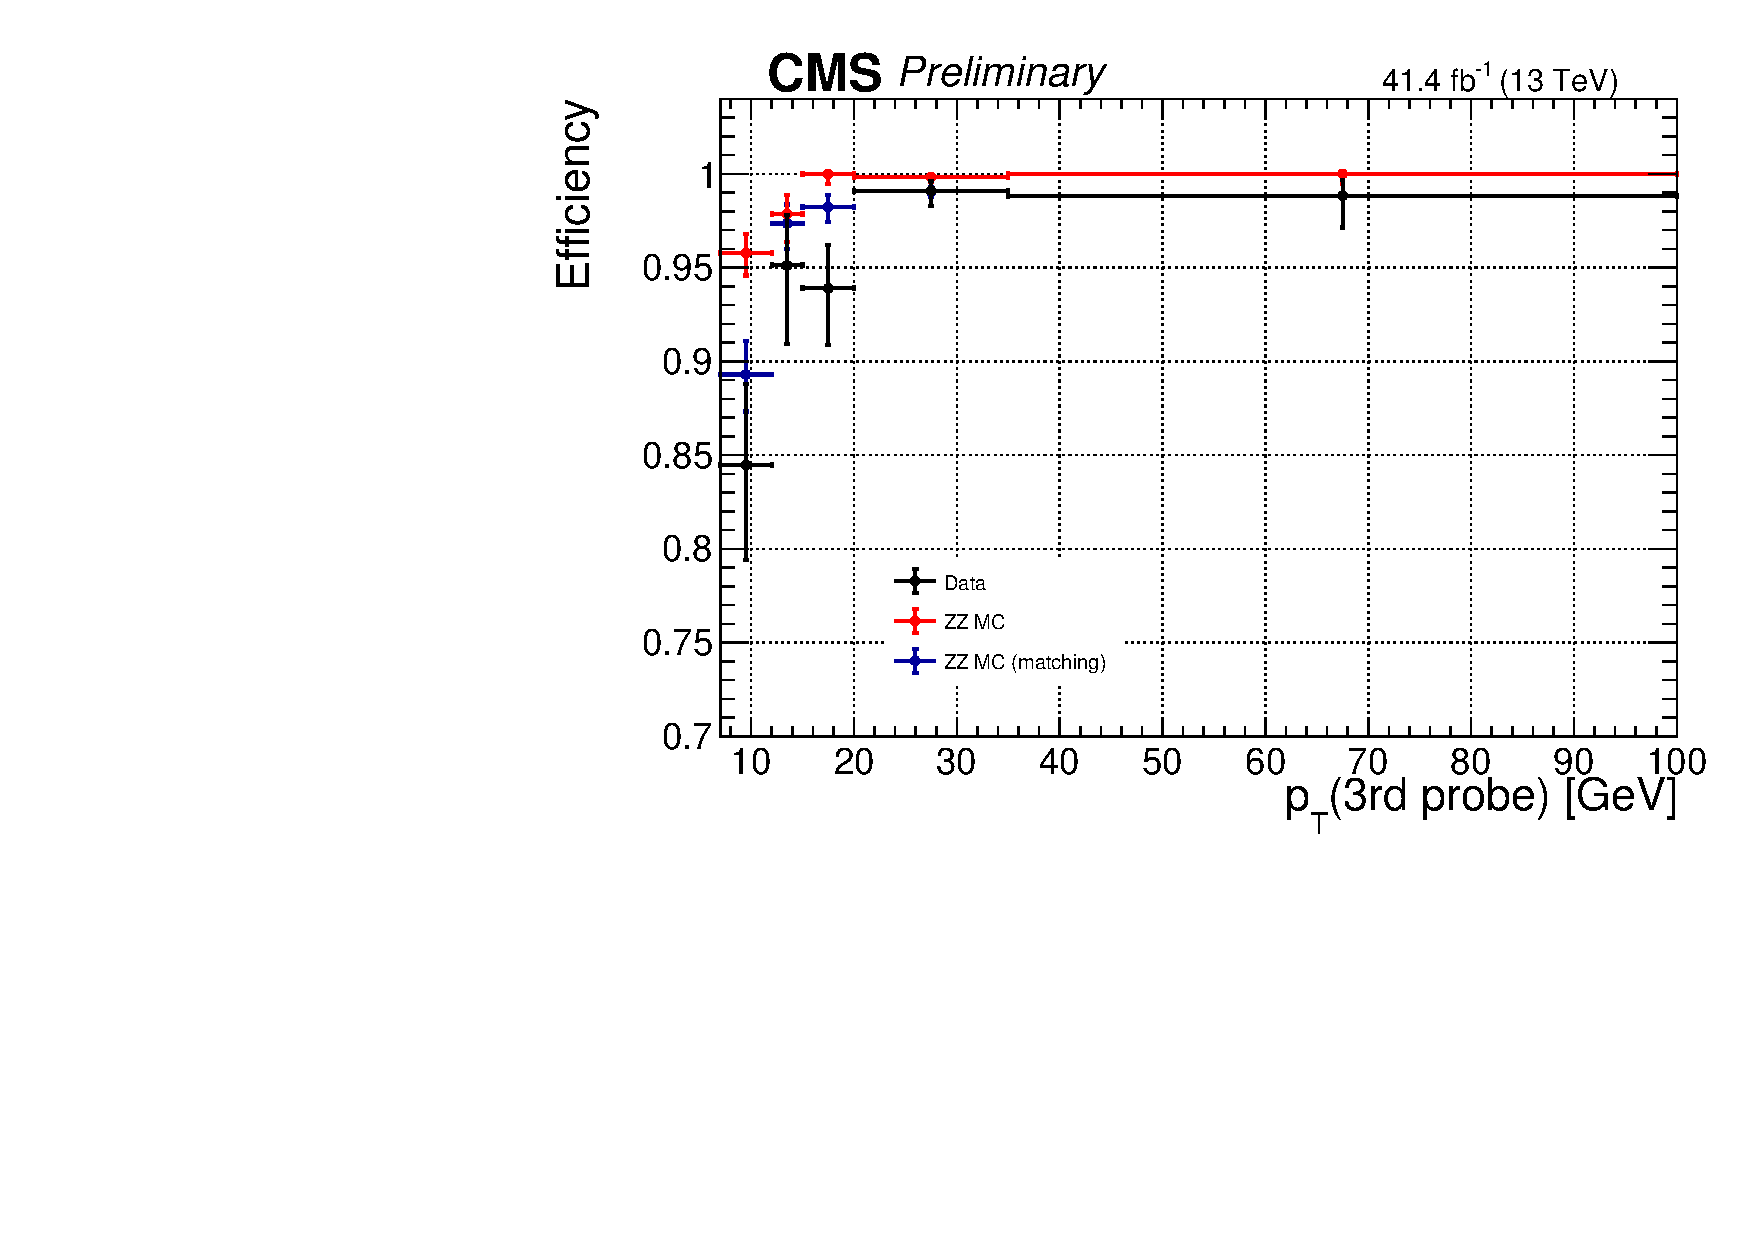
\includegraphics[width=0.45\textwidth]{Figures/Trigger/2017/Histo_TrigEff_ptMin_4e_mZ2_12.pdf} 
%		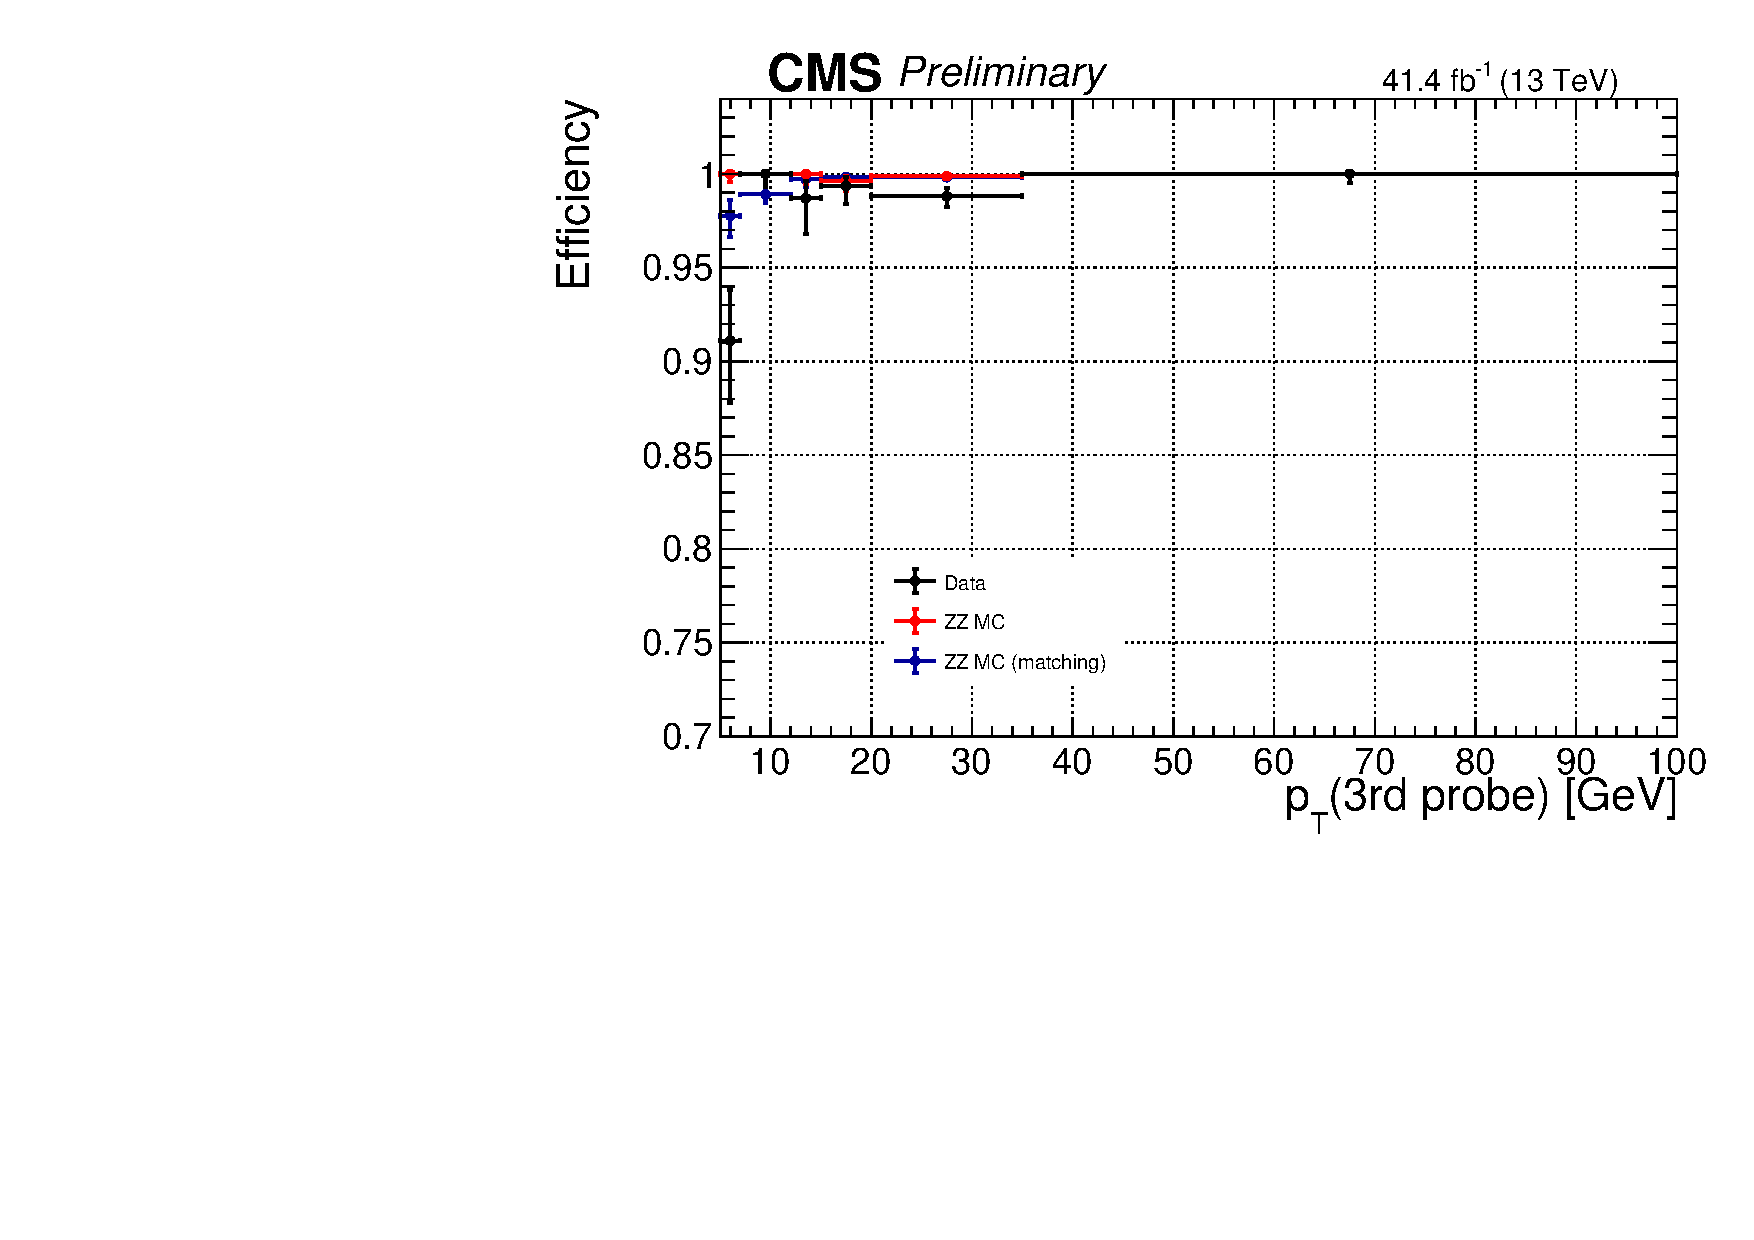
\includegraphics[width=0.45\textwidth]{Figures/Trigger/2017/Histo_TrigEff_ptMin_4mu_mZ2_12.pdf} \\
%		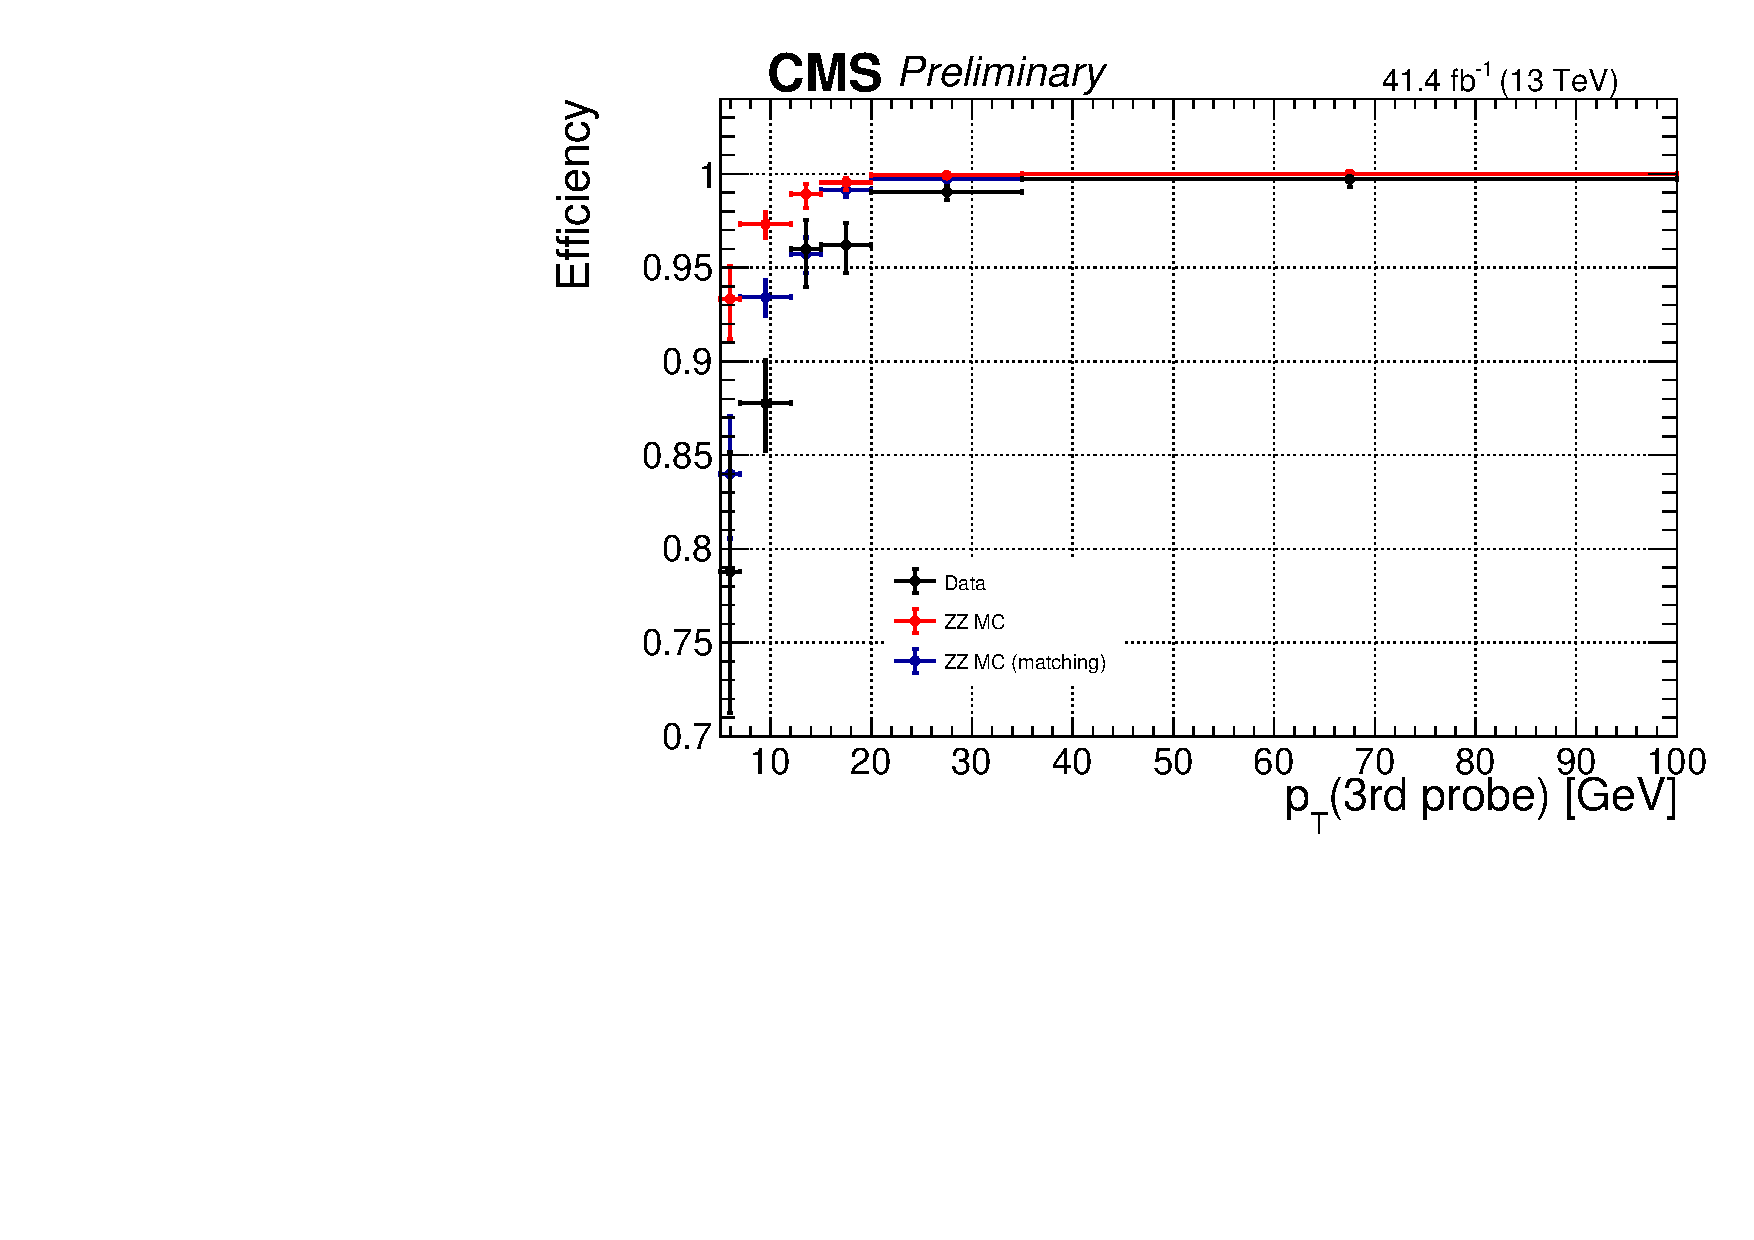
\includegraphics[width=0.45\textwidth]{Figures/Trigger/2017/Histo_TrigEff_ptMin_2e2mu_mZ2_12.pdf} 
%		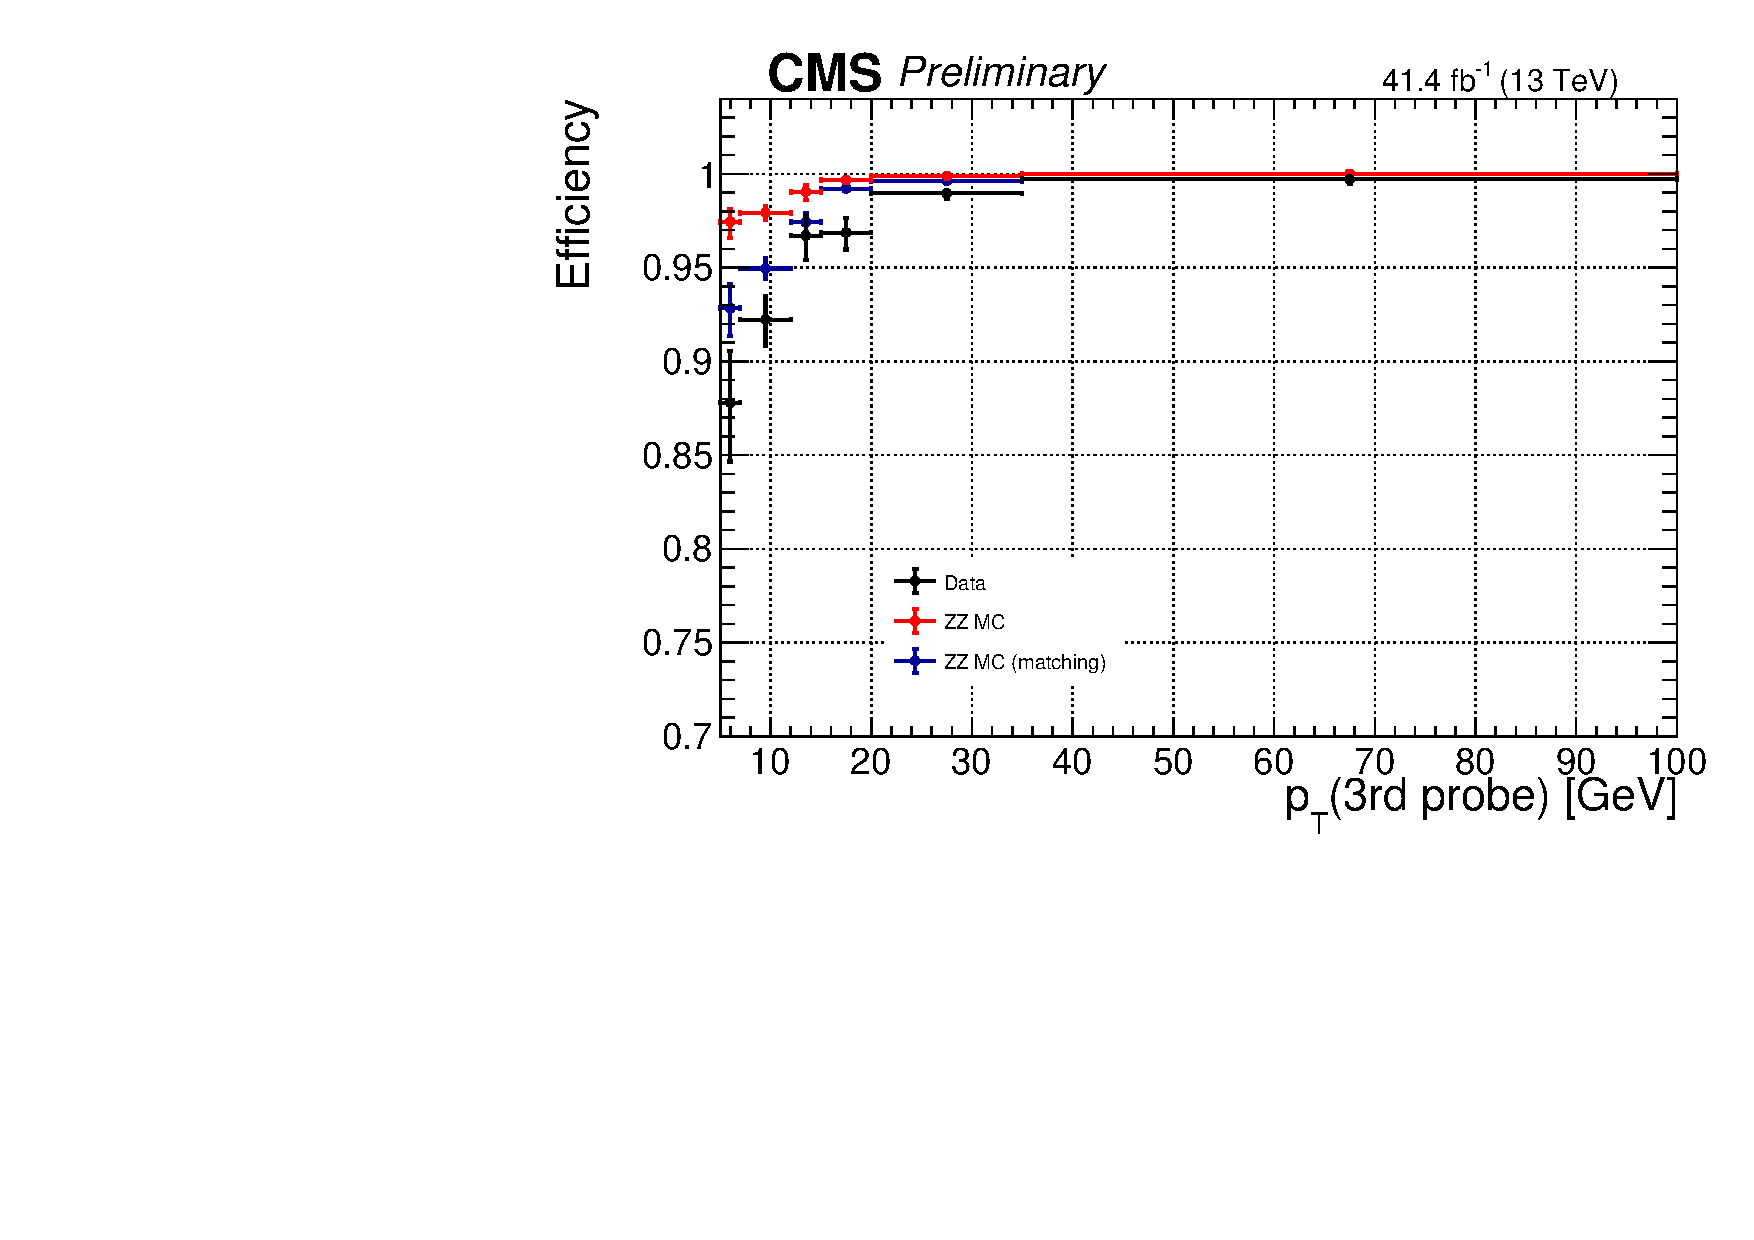
\includegraphics[width=0.45\textwidth]{Figures/Trigger/2017/Histo_TrigEff_ptMin_4l_mZ2_12.pdf} \\
%		\caption{Trigger efficiency measured in 2017 data using $4\ell$ events collected by single lepton triggers for the $4e$ (top left), $4\mu$ (top right), $2e2\mu$ (bottom left) and $4\ell$ (bottom right) final states. 
%			\label{fig:TrigEffB}}
%	\end{center}
%\end{figure}
%=======

%=======
%\begin{figure}[!htb]
%	\vspace*{0.3cm}
%	\begin{center}
%		\includegraphics[width=0.45\textwidth]{Figures/Trigger/Histo_TrigEff_ptMin_4e.pdf} 
%		\includegraphics[width=0.45\textwidth]{Figures/Trigger/Histo_TrigEff_ptMin_4mu.pdf} \\
%		\includegraphics[width=0.45\textwidth]{Figures/Trigger/Histo_TrigEff_ptMin_2e2mu.pdf} 
%		\includegraphics[width=0.45\textwidth]{Figures/Trigger/Histo_TrigEff_ptMin_4l.pdf} \\
%		\caption{ %\textbf{FIXME: Add figure once ready.}
%		Trigger efficiency measured in 2016 data using $4\ell$ events collected by single lepton triggers for the $4e$ (top left), $4\mu$ (top right), $2e2\mu$ (bottom left) and $4\ell$ (bottom right) final states. 
%			\label{fig:TrigEffC}}
%	\end{center}
%\end{figure}
%%=======

A summary of the trigger efficiencies in MC truth, and in MC and data using the tag and probe method are summarized in table~\ref{tab:TrigEffC}. The trigger efficiency in simulation is found to be $>99\%$ in each final state.

%\begin{table}[h]
%	\centering
%	\begin{tabular}{|c|c|c|c|c|} 
%		\hline %----------------------------------------------------------------
%		Final State  & $\ggH$ MC & $\ggH$ MC (matching)  & Data (matching)   \\
%		\hline %----------------------------------------------------------------
%		$4e$  & 0.991$^{+.002}_{-0.002}$ & 0.948$^{+.004}_{-0.004}$ & 0.982$^{+.005}_{-0.007}$ \\
%		$4\mu$  & 0.997$^{+.001}_{-0.001}$ & 0.997$^{+.001}_{-0.001}$ & 1.000$^{+.000}_{-0.001}$ \\
%		$2e2\mu$  & 0.995$^{+.001}_{-0.001}$ & 0.964$^{+.002}_{-0.002}$ & 0.983$^{+.003}_{-0.004}$ \\
%		\hline %----------------------------------------------------------------
%	\end{tabular}
%	\caption{Trigger efficiencies measured using $4\ell$ events in 2016 data.}
%	\label{tab:TrigEffA}
%\end{table}


%\begin{table}[h]
%    \centering
%    \begin{tabular}{|c|c|c|c|c|} 
%\hline %----------------------------------------------------------------
%Final State  & $\ggH$ MC & $\ggH$ MC (matching)  & Data (matching)   \\
%\hline %----------------------------------------------------------------
%$4e$  & 0.991$^{+.002}_{-0.002}$ & 0.948$^{+.004}_{-0.004}$ & 0.982$^{+.005}_{-0.007}$ \\
%$4\mu$  & 0.997$^{+.001}_{-0.001}$ & 0.997$^{+.001}_{-0.001}$ & 1.000$^{+.000}_{-0.001}$ \\
%$2e2\mu$  & 0.995$^{+.001}_{-0.001}$ & 0.964$^{+.002}_{-0.002}$ & 0.983$^{+.003}_{-0.004}$ \\
%\hline %----------------------------------------------------------------
%    \end{tabular}
%    \caption{Trigger efficiencies measured using $4\ell$ events in 2017 data.}
%    \label{tab:TrigEffB}
%\end{table}

\begin{table}[h]
	\centering
	\begin{tabular}{|c|c|c|c|c|} 
		\hline %----------------------------------------------------------------
		Final State  & $\ggH$ MC & $\ggH$ MC (matching)  & Data (matching)   \\
		\hline %----------------------------------------------------------------
		$4e$  & 0.991$^{+.002}_{-0.002}$ & 0.948$^{+.004}_{-0.004}$ & 0.982$^{+.005}_{-0.007}$ \\
		$4\mu$  & 0.997$^{+.001}_{-0.001}$ & 0.997$^{+.001}_{-0.001}$ & 1.000$^{+.000}_{-0.001}$ \\
		$2e2\mu$  & 0.995$^{+.001}_{-0.001}$ & 0.964$^{+.002}_{-0.002}$ & 0.983$^{+.003}_{-0.004}$ \\
		\hline %----------------------------------------------------------------
	\end{tabular}
	\caption{
	%\fixme{TO BE UPDATED, CURRENTLY COPY PASTE OF 2017 NUMBERS.}
		Trigger efficiencies measured using $4\ell$ events in 2018 data (TBU).}
	\label{tab:TrigEffC}
\end{table}

%\subsection{Simulation}
\subsection{Simulation samples}

\subsubsection{Signal Samples}

Descriptions of the SM Higgs boson production are obtained using the 
{\sc powheg V2}~\cite{Alioli:2008gx,Nason:2004rx,Frixione:2007vw} generator for the five main production modes: 
%gluon fusion ($\ggH$) including quark mass effects~\cite{Bagnaschi:2011tu}, vector boson fusion 
gluon fusion ($\ggH$) including quark mass effects~\cite{Bagnaschi:2011tu}, vector boson fusion 
(VBF)~\cite{Nason:2009ai}, and associated production (WH, $\cPZ$H and \ttbar$\,$H~\cite{Hartanto:2015uka}). 
The simulation of Higgs production through gluon fusion i.e. $\ggH$ production at next-to-next-to-leading order (NNLO) is obtained by {\sc NNLOPS} \cite{Hamilton:2013fea} and is used in the analysis as reference theory predictions for observed differential cross section results. A dedicated studies using {\sc MadGraph5\_aMC@NLO-FxFx} generators with next-to-leading order (NLO) accuracy is done for $\ggH$ production as additional theoretical predication for fiducial cross section measurement. Details are described in Section \ref{madgraph5}. 
In the case of WH and $\cPZ$H the {\sc MiNLO HVJ} extension of {\sc powheg} is used~\cite{Luisoni:2013kna}. 
The description of the decay of the Higgs boson to four leptons is obtained using the {\sc JHUgen} 
generator~\cite{Gao:2010qx}. In the case of WH, $\cPZ$H and \ttbar$\,$H, the Higgs boson is allowed
to decay to H$\to \cPZ \cPZ \to 2\ell2$X such that 4-lepton events where two leptons originate from 
the decay of associated $\cPZ$, W bosons or top quarks are also taken into account in the simulation. 
Showering of parton-level events is done using {\sc pythia8.209}, and in all cases matching is performed by 
allowing QCD emissions at all energies in the shower and vetoing them afterwards according to the 
{\sc powheg} internal scale. All samples are generated with the NNPDF 3.1 NLO parton distribution 
functions (PDFs)~\cite{Ball:2014uwa}. The list of signal samples and their cross sections are shown in 
Table~\ref{tab:SignalSamples}. For each year, corresponding simulation samples are reweighted to match the pileup distribution in data for which details are described in \cite{CMS-PAS-HIG-19-001}.

\begin{table}
\begin{scriptsize}
	\centering
    \begin{tabular}{|l|l|r|}
	\hline
 	Process & Dataset Name & $\sigma\times BR (\times\epsilon_{\text{filter}})$ \\ \hline
	$\rm{gg}\to\rm{H(124)}\to\cPZ\cPZ \to 4\ell$ & /GluGluHToZZTo4L\_M124\_13TeV\_powheg2\_JHUgenV7011\_pythia8/[1] & $12.18~\rm{fb}$ \\ % & $12.12~\rm{fb}$ \\
	$\rm{gg}\to\rm{H(125)}\to\cPZ\cPZ \to 4\ell$ & /GluGluHToZZTo4L\_M125\_13TeV\_powheg2\_JHUgenV7011\_pythia8/[1] & $12.18~\rm{fb}$ \\ % & $12.12~\rm{fb}$ \\
	$\rm{gg}\to\rm{H(126)}\to\cPZ\cPZ \to 4\ell$ & /GluGluHToZZTo4L\_M126\_13TeV\_powheg2\_JHUgenV7011\_pythia8/[1] & $12.18~\rm{fb}$ \\ % & $12.12~\rm{fb}$ \\
 	$\rm{qq}\to\rm{Hqq}\to\cPZ\cPZ\rm{qq}\to4\ell qq$ & /VBF\_HToZZTo4L\_M125\_13TeV\_powheg2\_JHUgenV709\_pythia8/[1] & $1.044~\rm{fb}$ \\ % $1.034~\rm{fb}$ \\
 	$\rm{q\bar{q}}\to\rm{W^{+}H}\to\rm{W^{+}}\cPZ\cPZ\to4\ell+\rm{X}$ & /WplusH\_HToZZTo4L\_M125\_13TeV\_powheg2-minlo-HWJ\_JHUgenV7011\_pythia8/[1] & $0.232~\rm{fb}$ \\ % $0.2339~\rm{fb}$ \\
 	$\rm{q\bar{q}}\to\rm{W^{-}H}\to\rm{W^{-}}\cPZ\cPZ\to4\ell+\rm{X}$ & /WminusH\_HToZZTo4L\_M125\_13TeV\_powheg2-minlo-HWJ\_JHUgenV7011\_pythia8/[1] & $0.147~\rm{fb}$ \\ % $0.1471~\rm{fb}$ \\
 	$\rm{q\bar{q}}\to\cPZ \rm{H}\to\cPZ\cPZ\cPZ\to4\ell+\rm{X}$ & /ZH\_HToZZ\_4LFilter\_M125\_13TeV\_powheg2-minlo-HZJ\_JHUgenV7011\_pythia8/[1] & $0.668~\rm{fb}$ \\ % $0.652~\rm{fb}$ \\
 	$\rm{gg}\to\rm{ttH} \to\rm{tt}\cPZ\cPZ\to4\ell+\rm{X}$ & /ttH\_HToZZ\_4LFilter\_M125\_13TeV\_powheg\_JHUgenV7011\_pythia8/[1] & $0.393~\rm{fb}$ \\ % $0.337~\rm{fb}$ \\ 
	$\rm{gg}\to\rm{bbH} \to\rm{bb}\cPZ\cPZ\to4\ell+\rm{X}$ & /bbH\_ToZZTo4L\_M125\_13TeV\_JHUGenV7011\_pythia8/[1] & $0.135~\rm{fb}$ \\
	$\rm{q\bar{q}}/\rm{qg}\to tHq \to tq\cPZ\cPZ\to4\ell+\rm{X}$ & /tqH\_HToZZTo4L\_M125\_13TeV\_JHUGenV7011\_pythia8/[1] & $0.0213~\rm{fb}$ \\
 	\hline
	\multicolumn{3}{l}{[1] HIG-RunIISummer20UL18wmLHEGEN-000*} \\  %TrancheIV\_v6-v1} \\
 	\end{tabular}
 	\caption{Signal Monte Carlo samples and cross sections.}
  	\label{tab:SignalSamples}
\end{scriptsize}
\end{table}

\subsubsubsection{\textbf{Simulation of Higgs production using {\sc madgraph5}}} \label{madgraph5}

To be updated.


\subsubsection{Background Samples}

Production of $ZZ$ via quark-antiquark annihilation is generated at
next-to-leading order (NLO) using {\sc powheg V2}~\cite{Nason:2013ydw}
and {\sc pythia8}, with 
the same settings as for the Higgs signal. As this simulation covers a large
range of ZZ invariant masses, dynamical QCD factorization and renormalization
scales have been chosen, equal to $m_{\cPZ\cPZ}$. 

The $\Pg\Pg \! \to \! ZZ$ process is simulated at leading order (LO) 
with MCFM~\cite{MCFM,Campbell:2013una}. In order to match the 
$\Pg\Pg \! \to \mathrm{H} \to \! ZZ$ transverse momentum spectra predicted 
by {\sc powheg} at NLO, the showering for MCFM samples is performed with 
different {\sc pythia8} settings, allowing only emissions up to the parton-level scale
(``wimpy'' shower).

Although not directly used to model data observations, additional 
MC samples of W$\cPZ$, Drell-Yan+jets, \ttbar, and tribosons are
generated using {\sc MadGraph5\_aMCatNLO}~\cite{Alwall:2014hca} either
inclusively or merging several jet multiplicities, as detailed in the table.
Table~\ref{tab:MCsamples} summarizes the MC simulation datasets used for this analysis. 


\begin{table}
\begin{footnotesize}
    \centering
    \begin{tabular}{|l|l|r|}
   \hline
 Process & Dataset Name & $\sigma\cdot BR$ \\ \hline
 $\rm{qq} \to \cPZ\cPZ \to 4\ell$ & /ZZTo4L\_TuneCP5\_13TeV\_powheg\_pythia8/ & $1.256~\rm{pb}$ \\
 $\rm{qq} \to \cPZ\cPZ \to 4\ell$ & /ZZTo4L\_TuneCP5\_13TeV-amcatnloFXFX-pythia8/ & $1.212~\rm{pb}$ \\
 $\rm{gg} \rightarrow \cPZ\cPZ \to 4e$ & /GluGluToContinToZZTo4e\_13TeV\_MCFM701/ & $0.00159~\rm{ pb}$ \\
 $\rm{gg} \rightarrow \cPZ\cPZ \to 4\mu$ & /GluGluToContinToZZTo4mu\_13TeV\_MCFM701/ & $0.00159~\rm{ pb}$ \\
 $\rm{gg} \rightarrow \cPZ\cPZ \to 2e2\mu$ & /GluGluToContinToZZTo2e2mu\_13TeV\_MCFM701/ & $0.00319~\rm{ pb}$ \\
 $\cPZ \to \ell\ell$ + jets & /DYJetsToLL\_M-50\_TuneCUETP8M1\_13TeV-amcatnloFXFX-pythia8/ & $6104~\rm{ pb}$ \\
 $\cPZ \to \ell\ell$ + jets  & /DYJetsToLL\_M-10to50\_TuneCUETP8M1\_13TeV-amcatnloFXFX-pythia8/ & $18610~\rm{ pb}$ \\ \hline
 W$\cPZ \to 3\ell\nu$ & /WZTo3LNu\_TuneCUETP8M1\_13TeV-powheg-pythia8/ & $4.430~\rm{ pb}$ \\ \hline
 $t\bar{t}$ & /TTJets\_TuneCUETP8M1\_13TeV-amcatnloFXFX-pythia8/ & $815.96~\rm{ pb}$ \\ 
 $t\bar{t} \to 2\ell2\nu 2b$ & /TTTo2L2Nu\_13TeV-powheg/ &  $87.31~\rm{pb}$ \\ 
\hline
$\cPZ\cPZ\cPZ$ & /ZZZ\_TuneCUETP8M1\_13TeV-amcatnlo-pythia8/ & 0.01398 pb \\
W$\cPZ\cPZ$ &  /WZZ\_TuneCUETP8M1\_13TeV-amcatnlo-pythia8/ & 0.05565 pb \\
WW$\cPZ$ & /WWZ\_TuneCUETP8M1\_13TeV-amcatnlo-pythia8/ & 0.1651 pb \\ 
\hline
$t\bar{t}$+$\cPZ\cPZ$ & /TTZZ\_TuneCUETP8M2T4\_13TeV-madgraph-pythia8/ & 0.001572 pb \\
$t\bar{t}$+WW & /TTWW\_TuneCUETP8M2T4_13TeV-madgraph-pythia8/ & 0.007883 pb \\
$t\bar{t}$+$\cPZ$ & /ttZJets\_13TeV\_madgraphMLM/ & 0.259 pb \\
\hline
 \end{tabular}
 \caption{Background Monte Carlo samples and cross sections.}
  \label{tab:MCsamples}
\end{footnotesize}
\end{table}


%\subsubsection{Pileup Reweighting}
%%\textbf{FIXME TO BE UPDATED}
%For each year, corresponding simulation samples are reweighted to match the pileup distribution in data, as shown on the Fig.~\ref{fig:puWeight2018}. The minimum bias cross-section used for each year is 69.2 mb.
%%=======
%\begin{figure}[!htb]
%	\vspace*{0.3cm}
%	\begin{center}
%		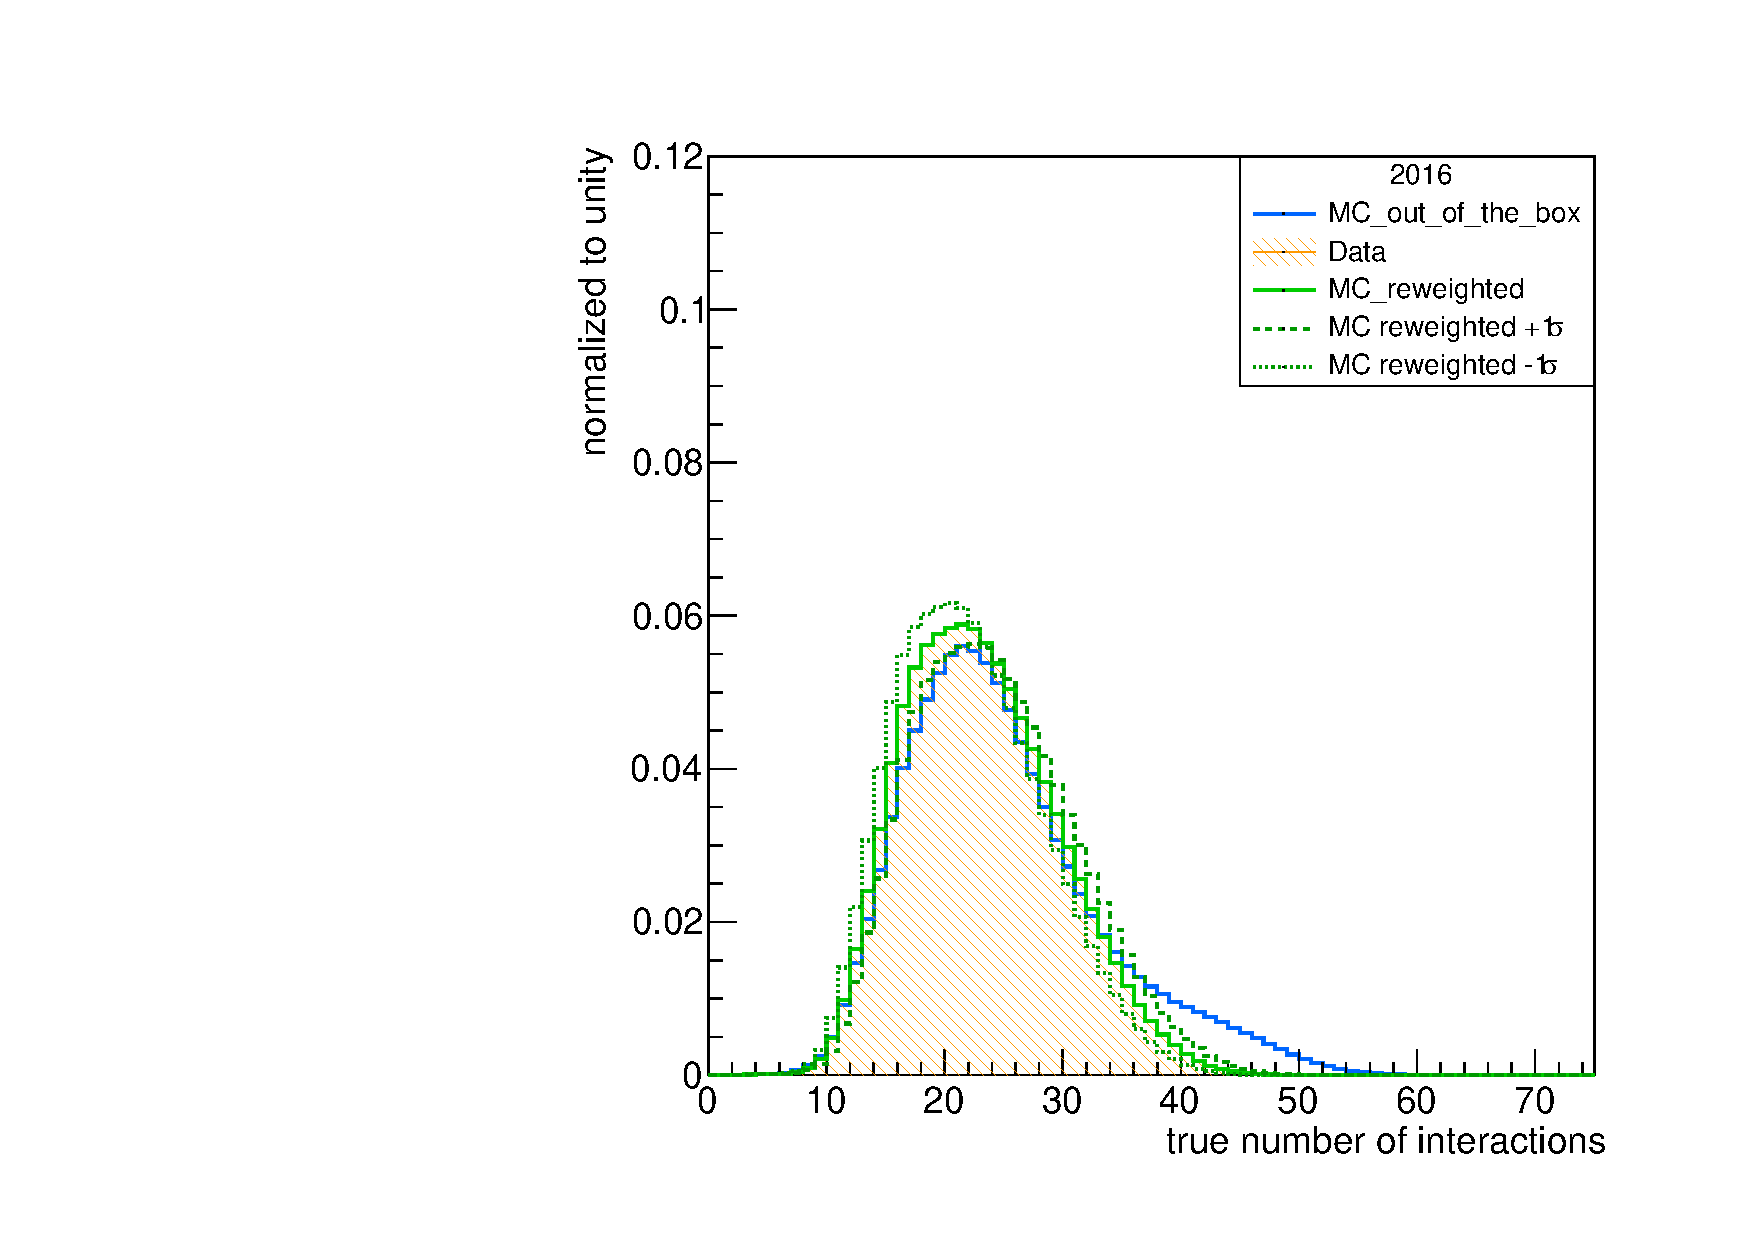
\includegraphics[width=0.45\textwidth]{Figures/PileUp/pu_weights_2016.pdf} \\
%                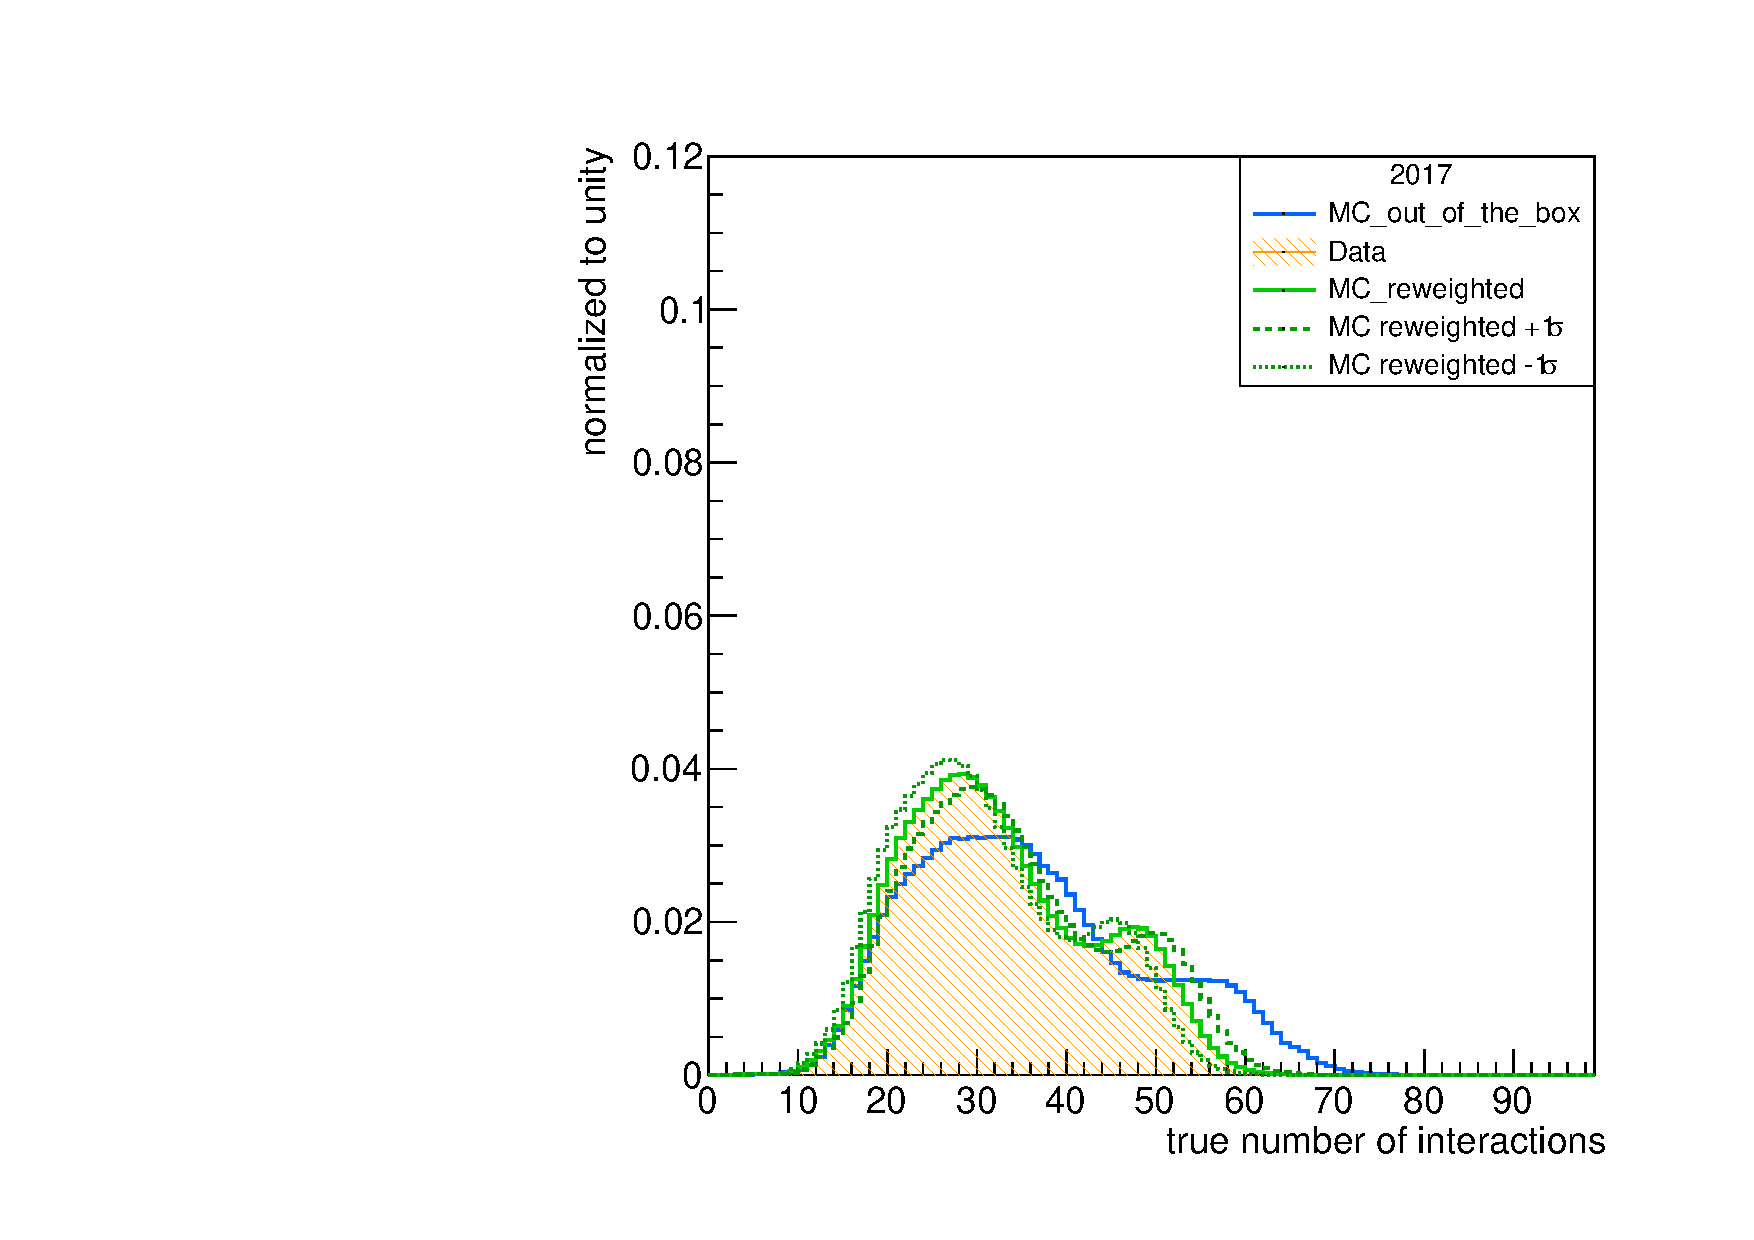
\includegraphics[width=0.45\textwidth]{Figures/PileUp/pu_weights_2017.pdf} \\
%                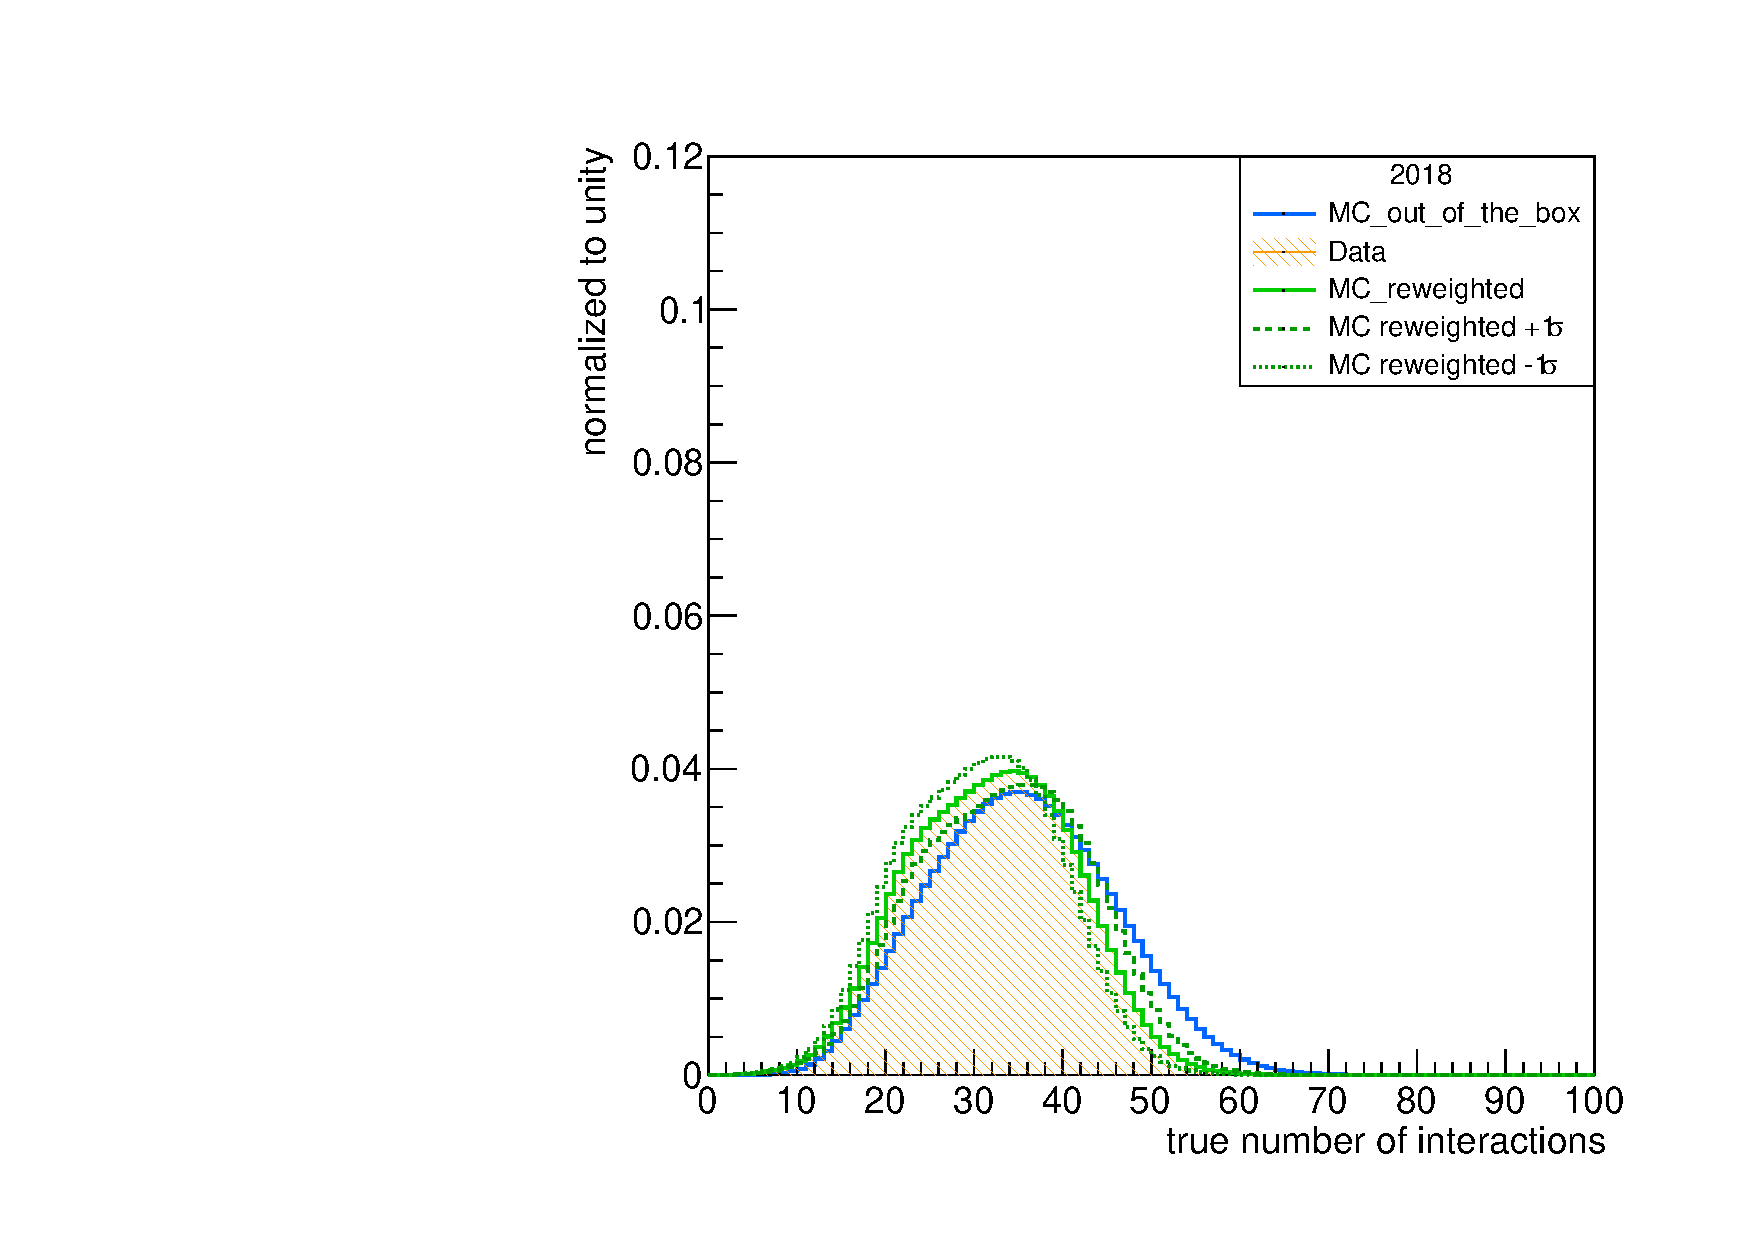
\includegraphics[width=0.45\textwidth]{Figures/PileUp/pu_weights_2018.pdf} \\
%		\caption{Distribution of pileup in 2016 (top), 2017 (middle) and 2018 (bottom) MC and Data shown before and after the application of PU weights. Up and down variations of 5\% in the minimum bias
%			cross section when calculating the weighs are also shown.
%			\label{fig:puWeight2018}}
%	\end{center}
%\end{figure}
%%=======

\subsection{Simulation samples for interpretations} \label{MCForInterpretations}
 %%% 
\clearpage
\section{Objects}
\label{sec:objects}
This analysis follows the same object defintion as in \cite{CMS:2019chr} for each year. Detailed descricption on objection definitions and scale factors can be found in the corresponding analysis note ~\cite{CMS-PAS-HIG-19-001}. Since this analysis is based on Ultra Legacy (UL) full Run 2 data, most of the objects related ingredients will be reevaluated with respect to ~\cite{CMS-PAS-HIG-19-001}.     

The reconstruction of the SM Higgs boson in the decay chain $\HZZfl$ requires very efficient lepton reconstruction and identification in order to be sensitive
to a low mass Higgs, for which at least one of the leptons has a $p_T$ within the range 5 - 15~GeV. In this kinematic region the need is for an optimal
efficiency, while retaining the rate of misidentified leptons low enough. On the same time, to allow a precise measurement of the Higgs boson mass and together
properties, which depend on the lepton kinematics, the analysis needs a precise momentum measurement. For both reasons, the analysis will make use of high
statistics sources of prompt leptons to measure efficiency, mis-identification rate, and energy scale/resolution. Muon Efficiency measuremens using UL dataset are discribed as follows:

%In this chapter we describe the selection of leptons and jets and the calibrations done on data control samples relevant for this analysis.
%
\subsection{Electrons}

%\subsubsection{Electron Reconstruction}
\subsubsection{Electron Reconstruction and Identification}
\label{sec:eleReco}
Referred to \cite{CMS-PAS-HIG-19-001}.

%More details on electron reconstruction can be found in Ref.~\cite{ElectronLegacy}. 
%
%Electron candidates are preselected using loose cuts on track-cluster matching observables, so as to preserve the highest possible efficiency while rejecting part of the QCD background. To be considered for the analysis, electrons are required to have a
%transverse momentum $p^e_T >$ 7 GeV, a reconstructed $|\eta^e| <$ 2.5, and to satisfy a loose primary vertex 
%constraint defined as $d_{xy} < 0.5$ cm and $d_z < 1$ cm.
%Such electrons are called {\bf loose electrons}.
%
%The data-MC discrepancy is corrected using scale factors as is done for the electron selection with data efficiencies measured using the same tag-and-probe technique outlined later (see Section~\ref{sec:eleEffMeas}). 
%These studies for reconstructions are carried out by the EGM POG and the results are only summarised here.
%
%The electron reconstruction scale factors are shown Fig.~\ref{fig:ele_rec_scale_factors} and are applied as a function of the super cluster $\eta$ and electron $\pt$.
%
%\begin{figure}[!htb]
%\vspace*{0.3cm}
%\begin{center}
%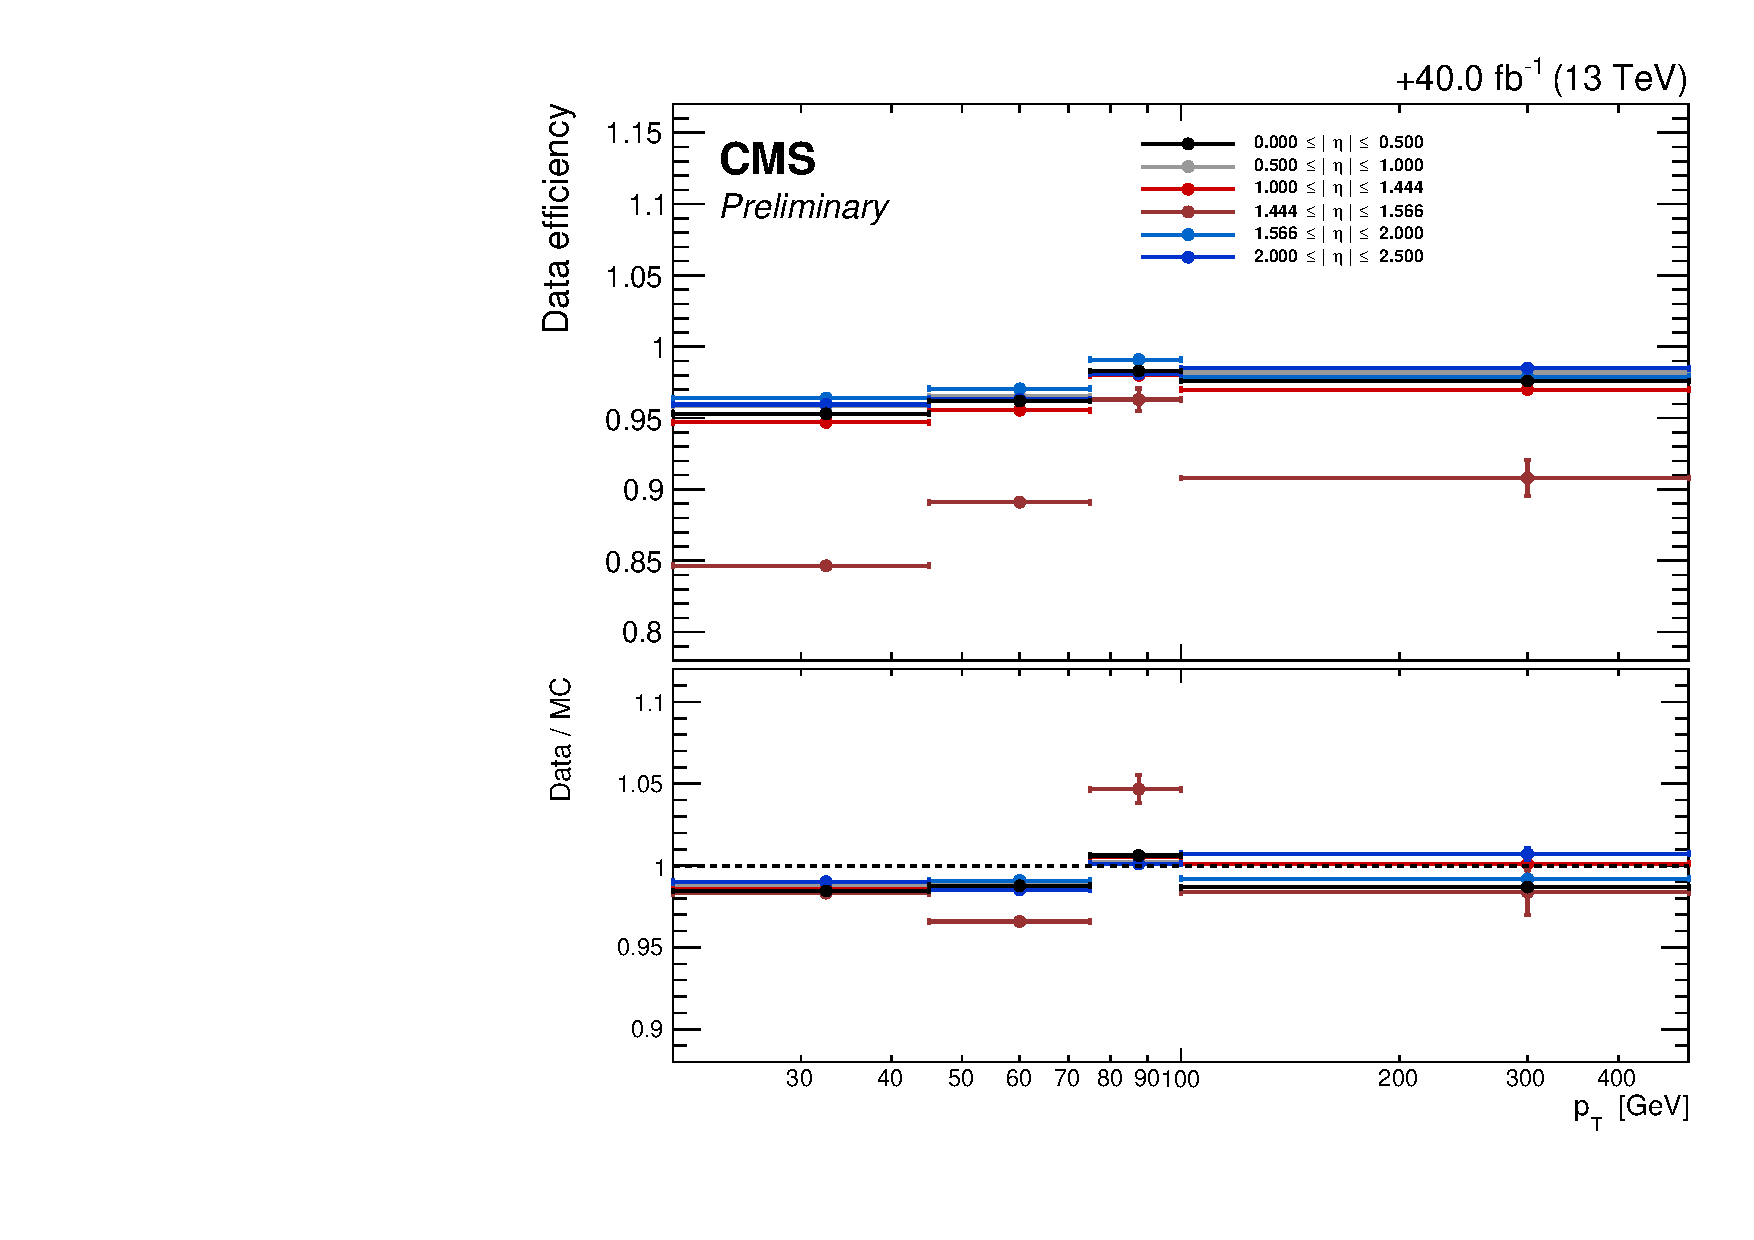
\includegraphics[width=0.4\textwidth]{Figures/Electrons/ErecoPt}
%\includegraphics[page=2, width=0.4\textwidth]{Figures/Electrons/ErecoEta}\\
%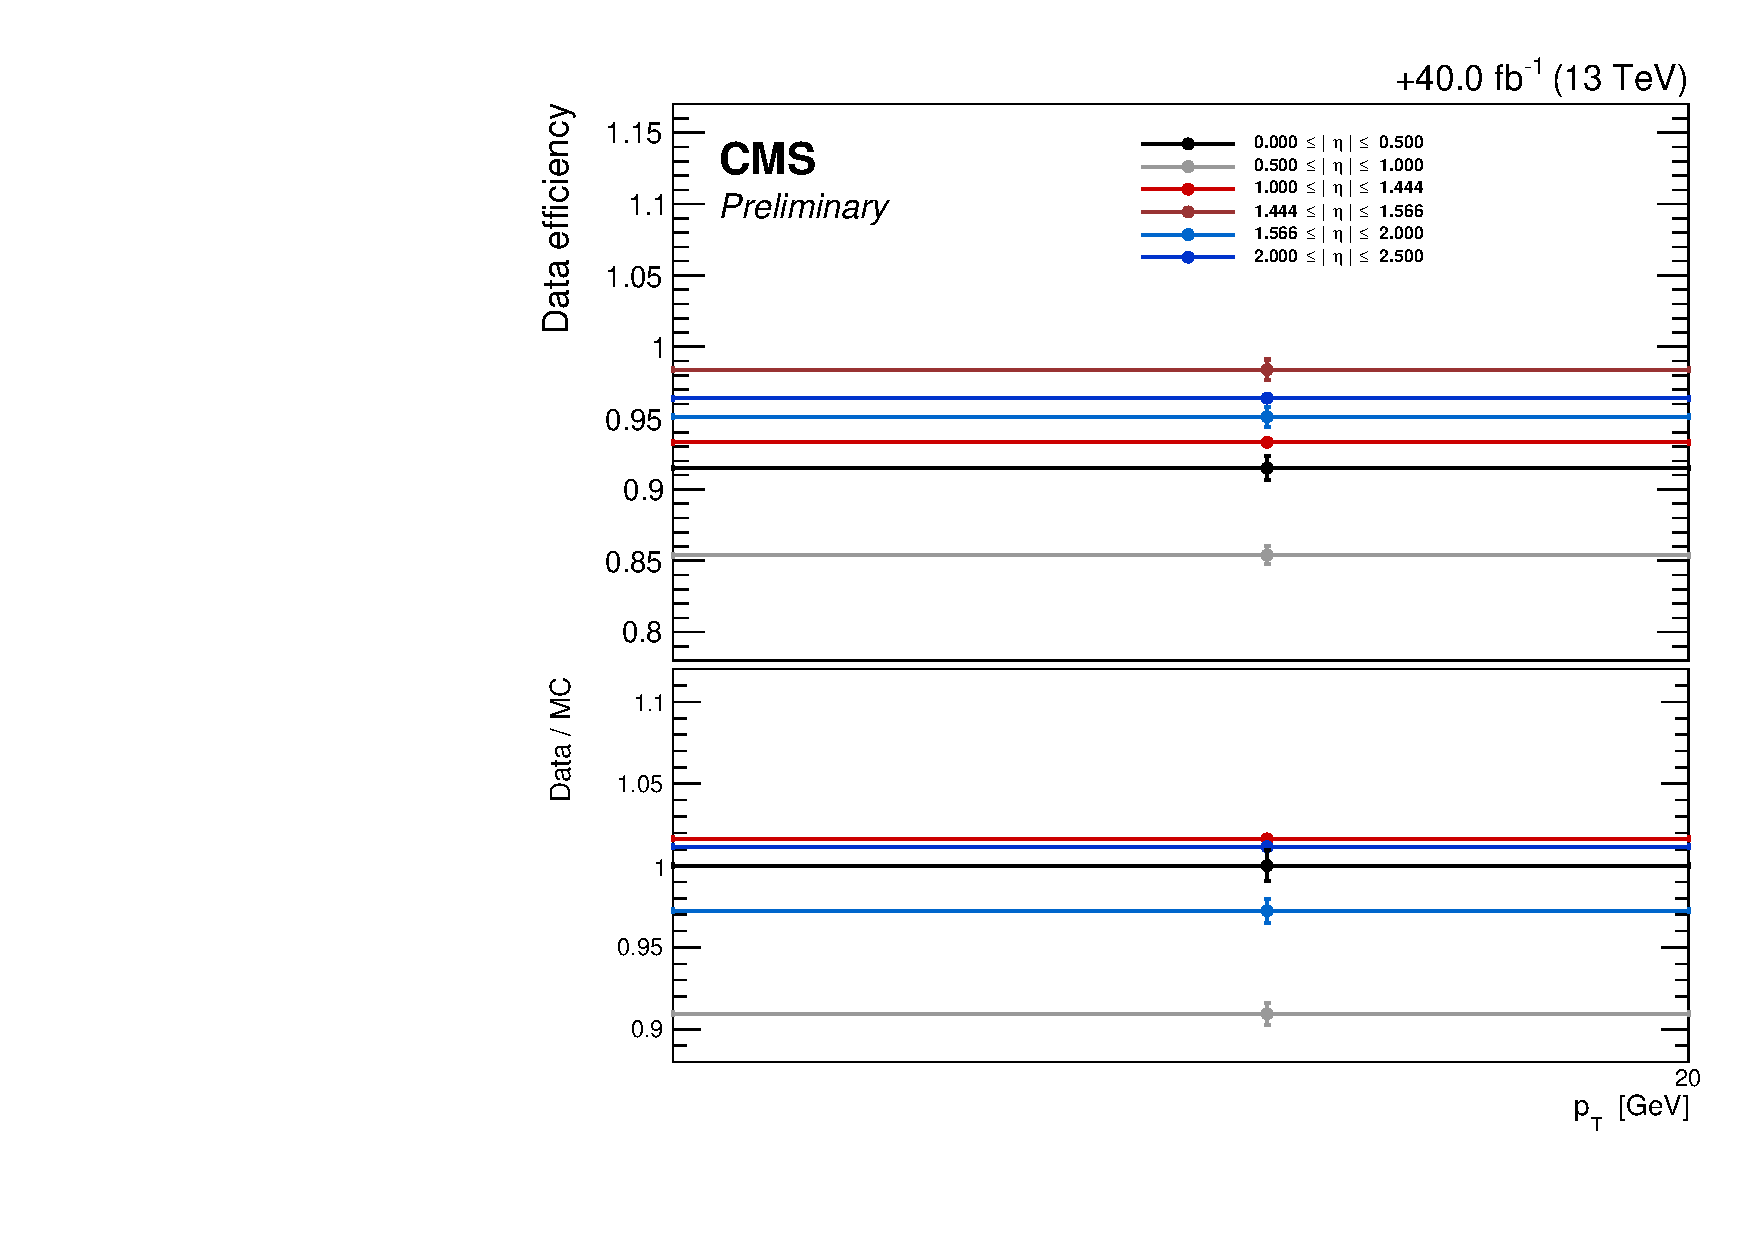
\includegraphics[width=0.4\textwidth]{Figures/Electrons/ErecoPt_lowPt}
%%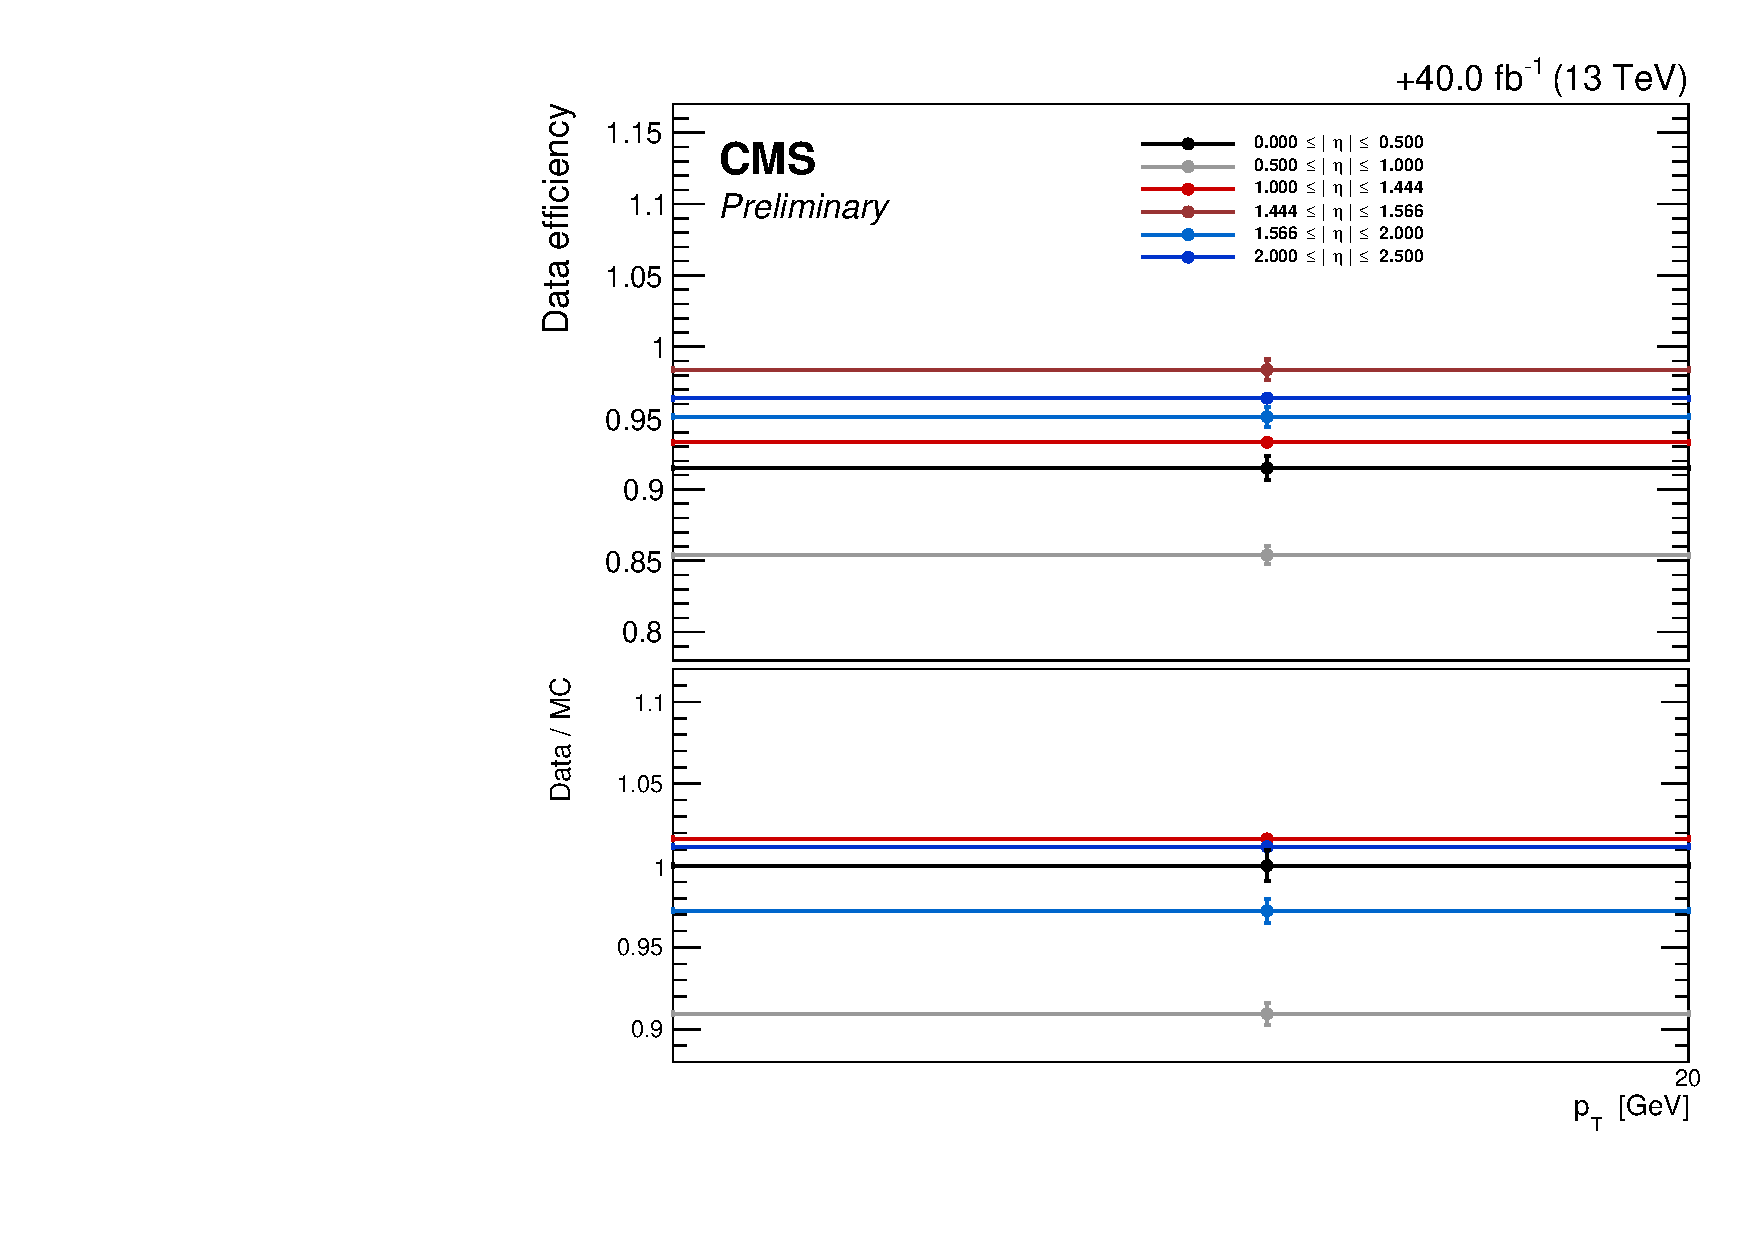
\includegraphics[width=0.4\textwidth]{Figures/Electrons/ErecoEta_lowPt}
%\end{center}
%\caption{Electron reconstruction efficiencies efficiency in data versus $p_T$ (left) and $\eta$ (right) for electrons with $\pt > 20 \GeV$ (top) and $\pt < 20 \GeV$ (bottom) with corresponding data/MC scale factors as provided by the EGM POG. Errors are statistical only. }
%\label{fig:ele_rec_scale_factors}
%\end{figure}
%


%
%\subsubsection{Electron Identification and Isolation}
%\label{sec:ele_MVA}
%One of the main improvements brought in the analysis is the usage of a new multivariate discriminant for electron selection in all data taking periods.

Reconstructed electrons are now identified and isolated by means of an e\textbf{X}treme \textbf{G}radient \textbf{Boost}ing (XGBoost) optimized distributed
gradient boosting library designed to be highly efficient, flexible and portable. It implements machine learning algorithms under the Gradient Boosting framework
and exploits observables from the electromagnetic cluster, the matching between the cluster and the electron track, observables based exclusively on tracking
measurements as well as particle flow isolation sums. The full list of used features can be found in the Table~\ref{tab:ele_ID_input_variables}.

\begin{table}[H]
\scriptsize
   \centering
   \begin{tabular}{c|l}
\hline
\hline
Observable type & Observable name \\
\hline
\multirow{6}{*}{Cluster shape}
	& RMS of the energy-crystal number spectrum along $\eta$ and $\varphi$; $\sigma_{i\eta i\eta}$, $\sigma_{i\varphi i\varphi}$ \\
	& Super cluster width along $\eta$ and $\phi$ \\
	& Ratio of the hadronic energy behind the electron supercluster to the supercluster energy, $H/E$ \\
	& Circularity $(E_{5\times5} - E_{5\times1})/E_{5\times5}$ \\
	& Sum of the seed and adjacent crystal over the super cluster energy $R_{9}$ \\
	& For endcap traing bins: energy fraction in pre-shower $E_\text{PS}/E_\text{raw}$ \\
\hline
\multirow{2}{*}{Track-cluster matching}
	& Energy-momentum agreement $E_{tot}/p_{in}$, $E_{ele}/p_{out}$, $1/E_{tot} - 1/p_{in}$ \\
	& Position matching $\Delta\eta_{in}$, $\Delta\varphi_{in}$, $\Delta\eta_{seed}$ \\
\hline
\multirow{5}{*}{tracking}
   & Fractional momentum loss $f_{brem} = 1 - p_{out}/p_{in}$ \\
   & Number of hits of the KF and GSF track $N_{KF}$, $N_{GSF}$ \\ %$(\mathord{\cdot})$ \\
   & Reduced $\chi^2$ of the KF and GSF track $\chi^{2}_{KF}$, $\chi^{2}_{\textrm{GSF}}$ \\
   & Number of expected but missing inner hits \\ %$(\mathord{\cdot})$ \\
   & Probability transform of conversion vertex fit $\chi^2$ \\ % $(\mathord{\cdot})$ \\
\hline
\multirow{3}{*}{isolation}
   & Particle Flow photon isolation sum \\ %$(\mathord{\cdot})$ \\
   & Particle Flow charged hadrons isolation sum \\ %$(\mathord{\cdot})$ \\
   & Particle Flow neutral hadrons isolation sum \\ %$(\mathord{\cdot})$ \\
\hline
\multirow{1}{*}{For PU-resilience}
   & Mean energy density in the event: $\rho$ \\ %$(\mathord{\cdot})$ \\
\hline
\hline
     \end{tabular}
\small
    \caption{Overview of input features to the identification classifier.} %Variables not used in the Run 2 MVA are marked with  $(\mathord{\cdot})$.}
    \label{tab:ele_ID_input_variables}
\end{table}


The model is trained on 2016, 2017, and 2018 Drell-Yan with jets MC sample for both signal and background. The separate training for three periods guarantees
optimal performance during the whole Run 2 data taking period. The simulated samples used to train the model are listed bellow.

\begin{itemize}
\item \textbf{2016} \begin{verbatim}/DYJetsToLL_M-50_TuneCUETP8M1_13TeV-amcatnloFXFX-pythia8/RunIISummer16MiniAODv2-PUMoriond17_80X_mcRun2_asymptotic_2016_TrancheIV_v6_ext2-v1/MINIAODSIM\end{verbatim}
\item \textbf{2017} \begin{verbatim}/DYJetsToLL_M-50_TuneCP5_13TeV-madgraphMLM-pythia8/RunIIFall17MiniAOD-RECOSIMstep_94X_mc2017_realistic_v10-v1/MINIAODSIM\end{verbatim}
\item \textbf{2018} \begin{verbatim}/DYJetsToLL_M-50_TuneCP5_13TeV-madgraphMLM-pythia8/RunIIAutumn18MiniAOD-102X_upgrade2018_realistic_v15-v1/MINIAODSIM\end{verbatim}
\end{itemize}

Several studies have been conducted on 2016 Drell-Yan with jets MC sample. The XGBoost framework was first used in 2017 and the model was trained on 2017
Drell-Yan with jets MC sample. This model is known as 2017 ID+ISO V2. The same framework was then used to train the model on 2016 MC (2016 ID+ISO) and finally
on 2018 MC (2018 ID+ISO). In Fig.~\ref{fig:ele_ID_ISO_ROC_2016} one can see the ROC curves obtained using 2016 Drell-Yan with jets MC sample. As expected, the
model trained on 2016 MC using electron identification and isolation features outperforms the model trained on 2016 MC using only identification features and
the model obtained after applying 2017 ID+ISO V2 training on 2016 Drell-Yan with jets MC sample.

In Fig.~\ref{fig:ele_ID_ISO_ROC_2016_} one can see the ROC curve for the model trained on 2016 MC using electron identification and isolation features and ROC
curve when applying sequential approach meaning applying isolation cut after cutting on the distribution obtained by training using only identification features.
As expected, the model obtained using electron identification and isolation features outperforms the sequential approach model.

\begin{figure}[!htb]
   \vspace*{0.3cm}
   \begin{center}
      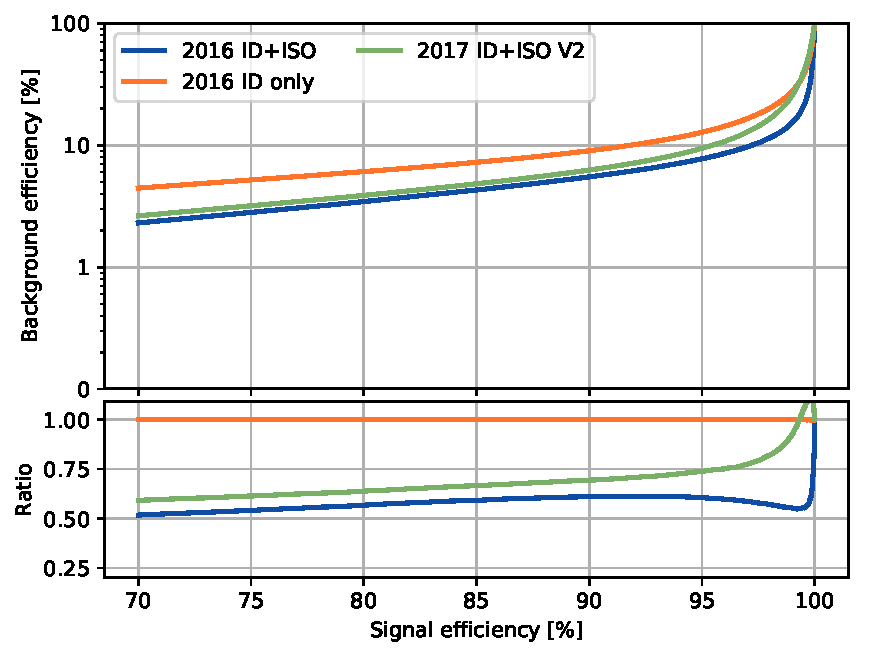
\includegraphics[width=0.45\textwidth]{Figures/Electrons/2016_EB1_5.pdf}
      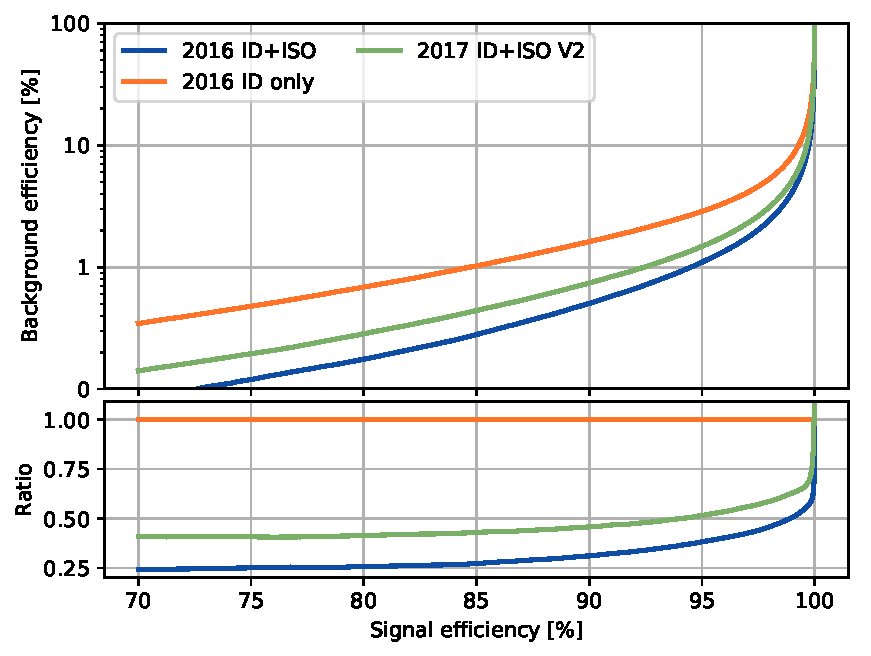
\includegraphics[width=0.45\textwidth]{Figures/Electrons/2016_EB1_10.pdf} \\
      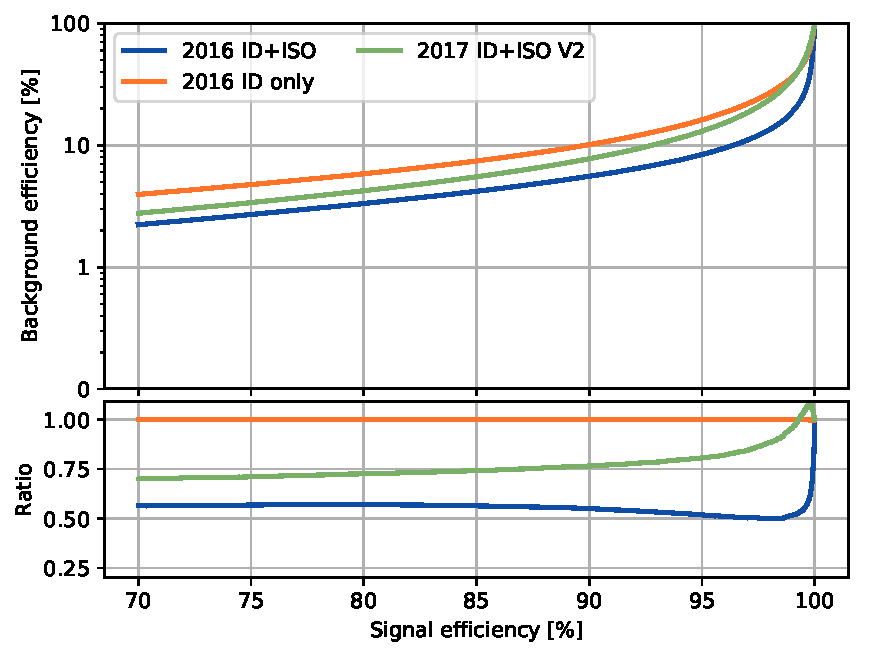
\includegraphics[width=0.45\textwidth]{Figures/Electrons/2016_EB2_5.pdf}
      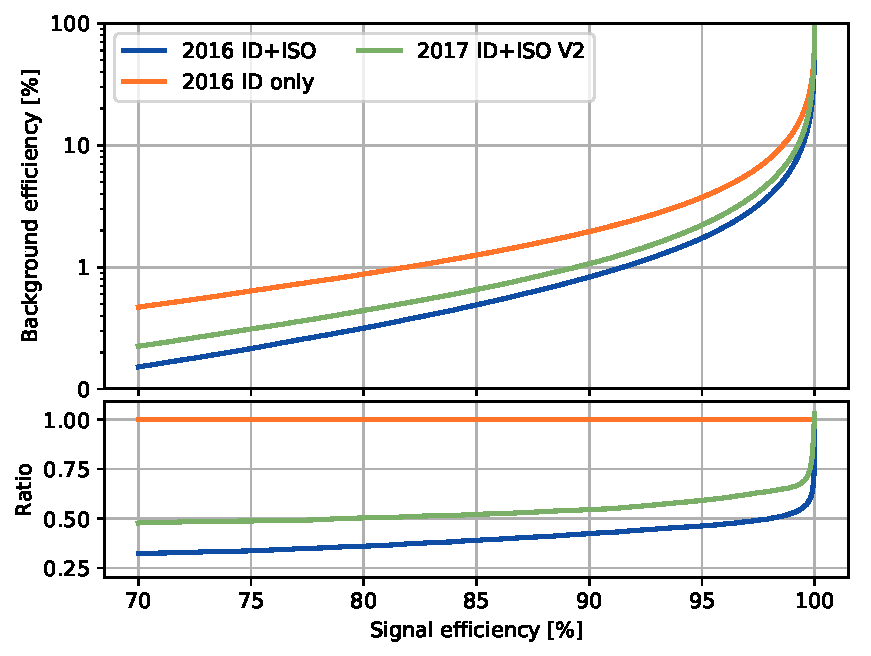
\includegraphics[width=0.45\textwidth]{Figures/Electrons/2016_EB2_10.pdf} \\
      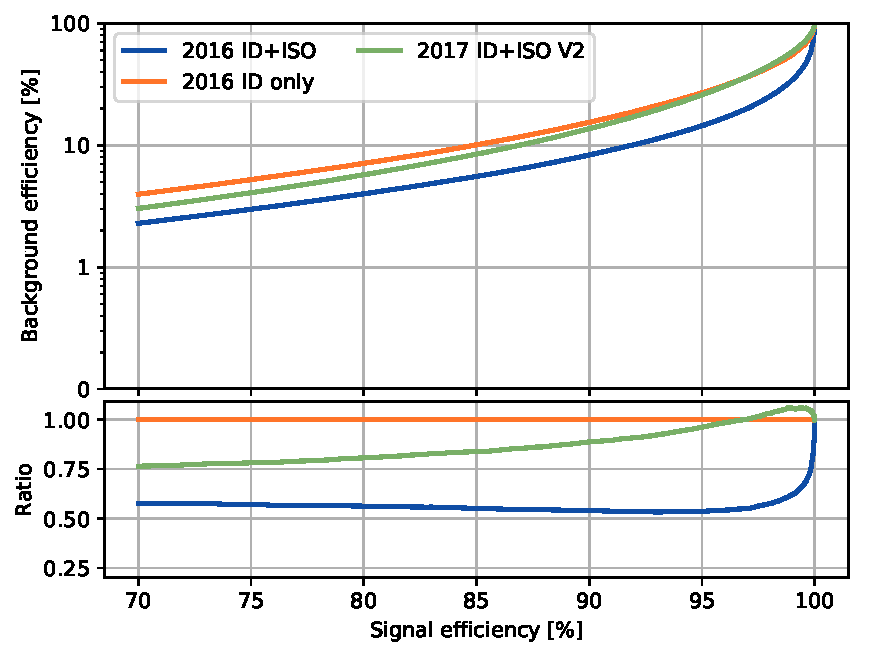
\includegraphics[width=0.45\textwidth]{Figures/Electrons/2016_EE_5.pdf}
      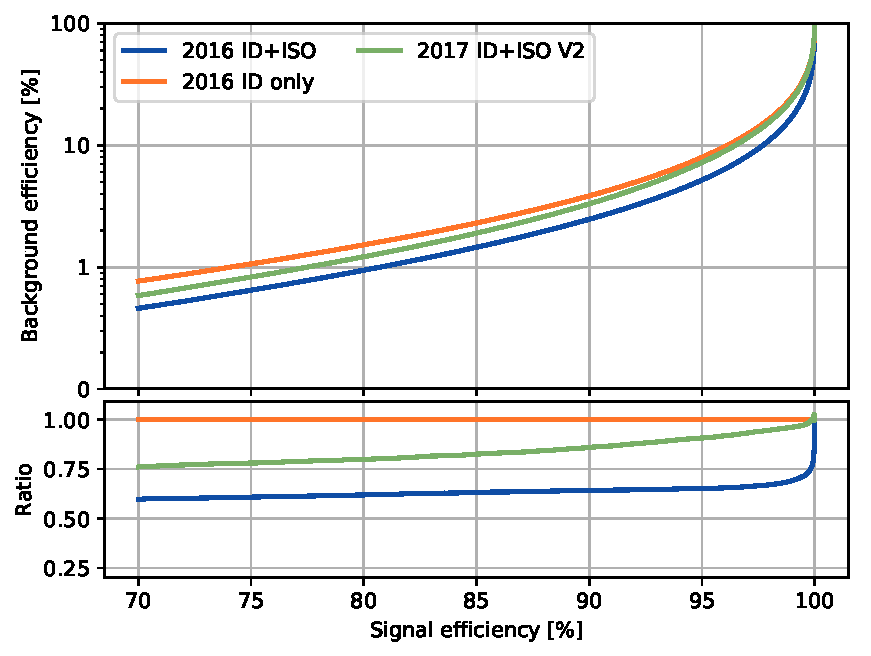
\includegraphics[width=0.45\textwidth]{Figures/Electrons/2016_EE_10.pdf} \\
   \caption{The receiver operating characteristic curves, representing the background efficiency vs signal efficiency, of the MVA trained on 2016 Drell-Yan with
   jets MC sample. Performance are shown for electrons with $5 < p_T < 10 $ GeV (left), $p_T > 10$ GeV (right), and $|\eta| < 0.8$ (top),
   $0.8 < |\eta| < 1.479$ (middle), and $|\eta| > 1.479$ (bottom).
   \label{fig:ele_ID_ISO_ROC_2016}}
   \end{center}
\end{figure}


\begin{figure}[!htb]
   \vspace*{0.3cm}
   \begin{center}
      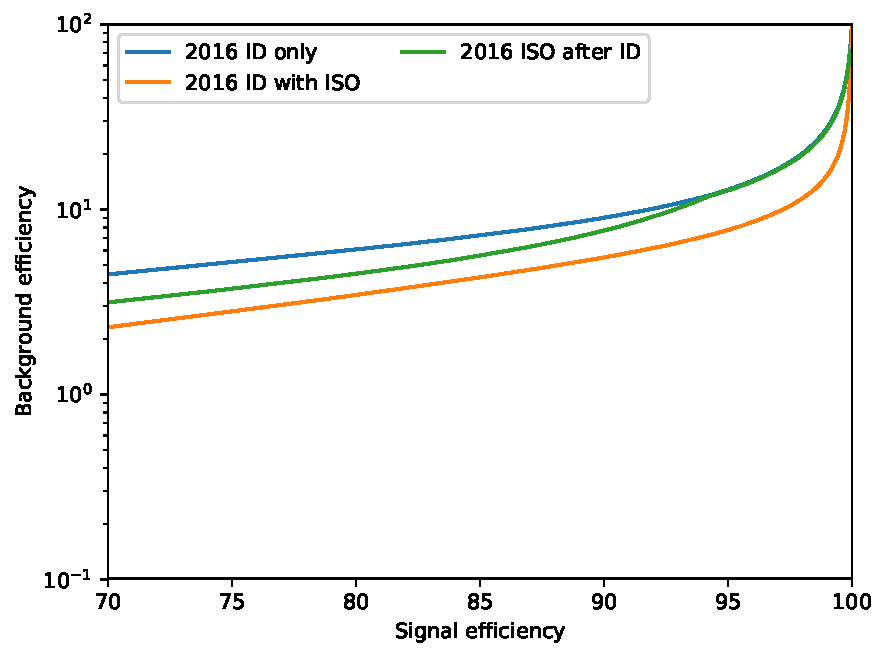
\includegraphics[width=0.45\textwidth]{Figures/Electrons/2016_EB1_5_.pdf}
      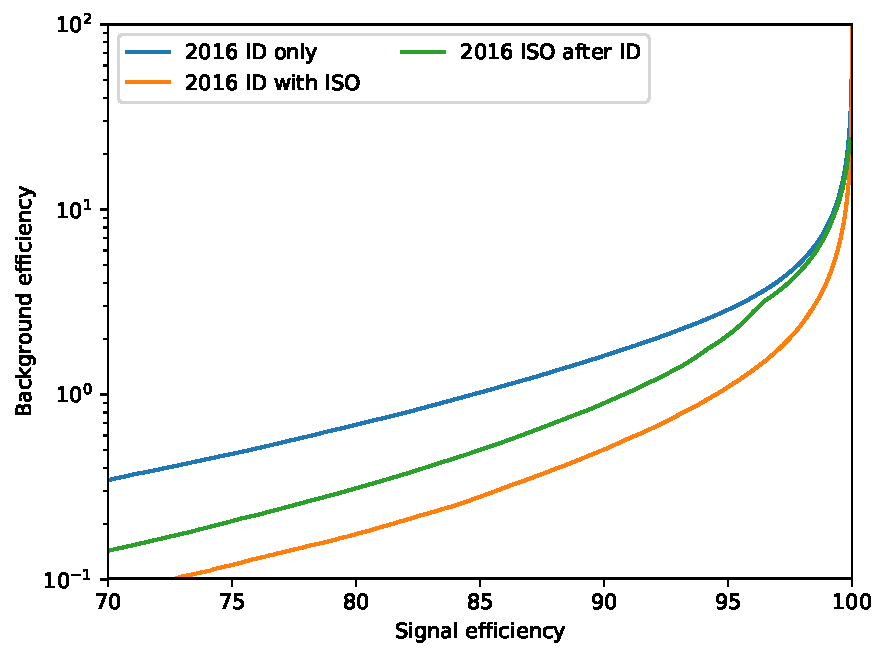
\includegraphics[width=0.45\textwidth]{Figures/Electrons/2016_EB1_10_.pdf} \\
      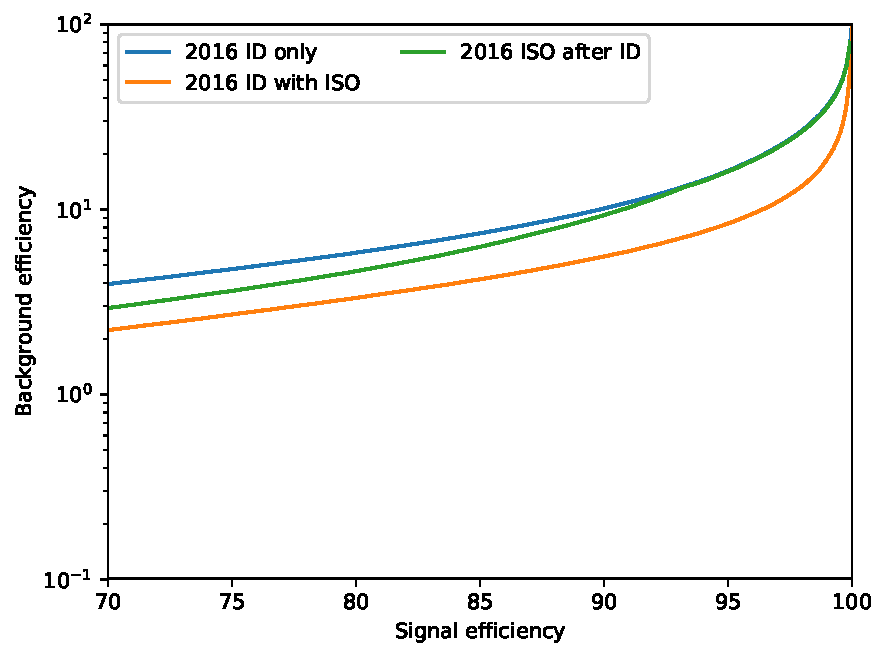
\includegraphics[width=0.45\textwidth]{Figures/Electrons/2016_EB2_5_.pdf}
      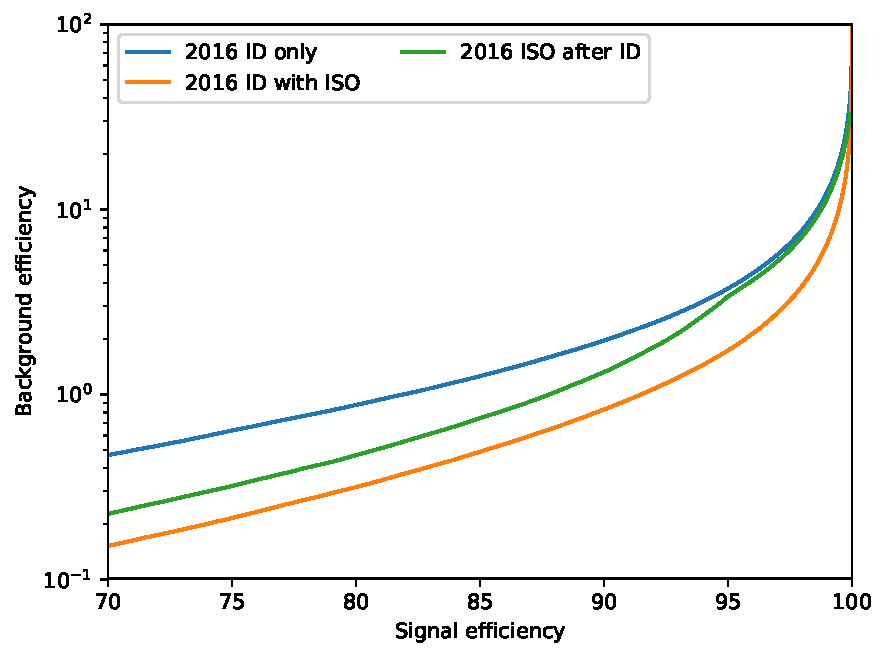
\includegraphics[width=0.45\textwidth]{Figures/Electrons/2016_EB2_10_.pdf} \\
      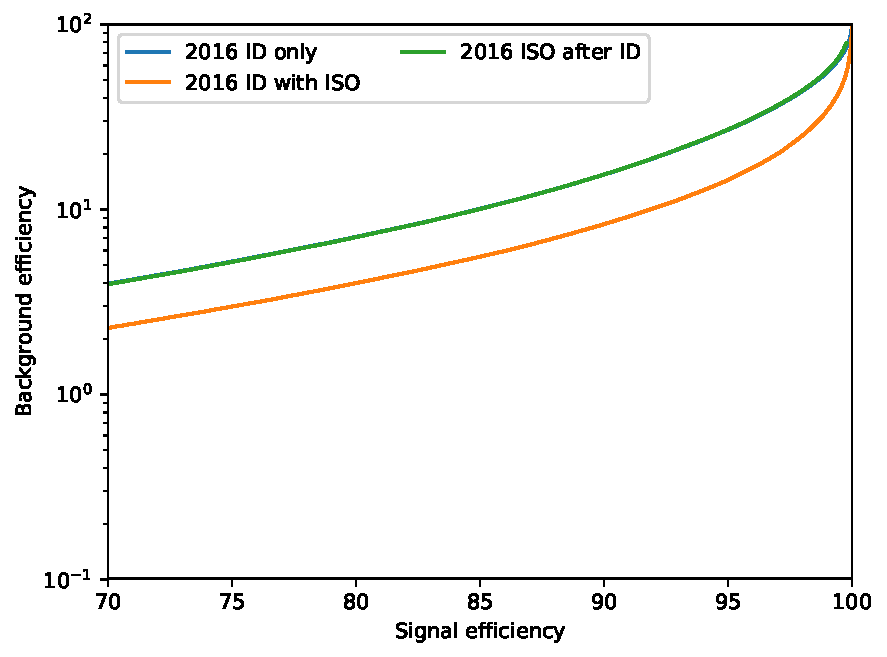
\includegraphics[width=0.45\textwidth]{Figures/Electrons/2016_EE_5_.pdf}
      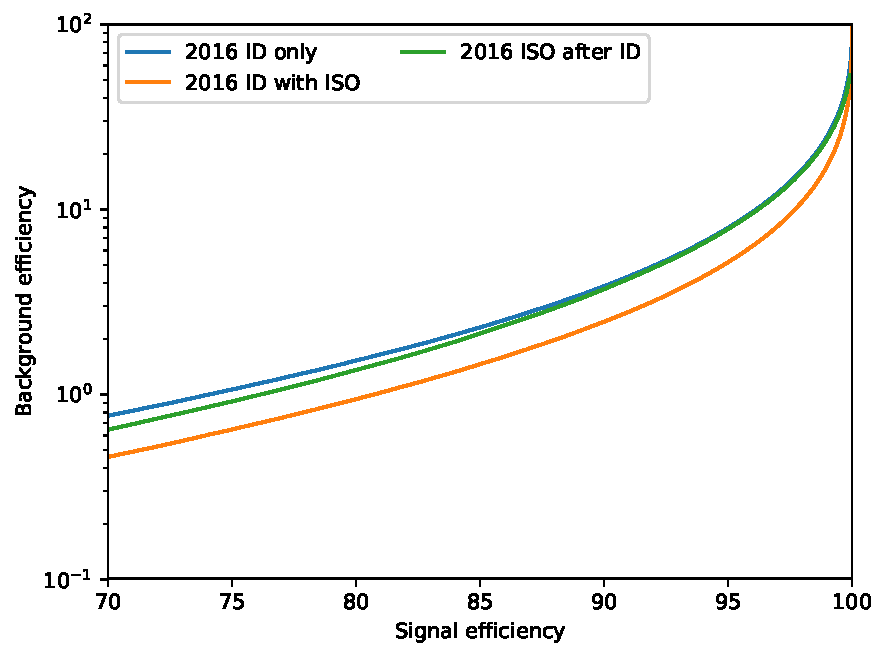
\includegraphics[width=0.45\textwidth]{Figures/Electrons/2016_EE_10_.pdf} \\
   \caption{The receiver operating characteristic curves, representing the background efficiency vs signal efficiency, of the MVA trained on 2016 Drell-Yan with
   jets MC sample. Performance are shown for electrons with $5 < p_T < 10 $ GeV (left), $p_T > 10$ GeV (right), and $|\eta| < 0.8$ (top),
   $0.8 < |\eta| < 1.479$ (middle), and $|\eta| > 1.479$ (bottom).
   \label{fig:ele_ID_ISO_ROC_2016_}}
   \end{center}
\end{figure}

The Fig.~\ref{fig:ele_MVA_score_2018} shows output of the multiclassifier discriminant i.e. MVA score for prompt electrons from Drell-Yan events and
misidentified electrons originating from jets in Drell-Yan events. The performance of  model trained on 2018 MC using electron identification and isolation
features outperforms the model obtained after applying 2017 ID+ISO V2 training on 2018 Drell-Yan with jets MC sample as shown in Fig.~\ref{fig:ele_ID_ISO_ROC_2018}.

\begin{figure}[!htb]
   \vspace*{0.3cm}
   \begin{center}
      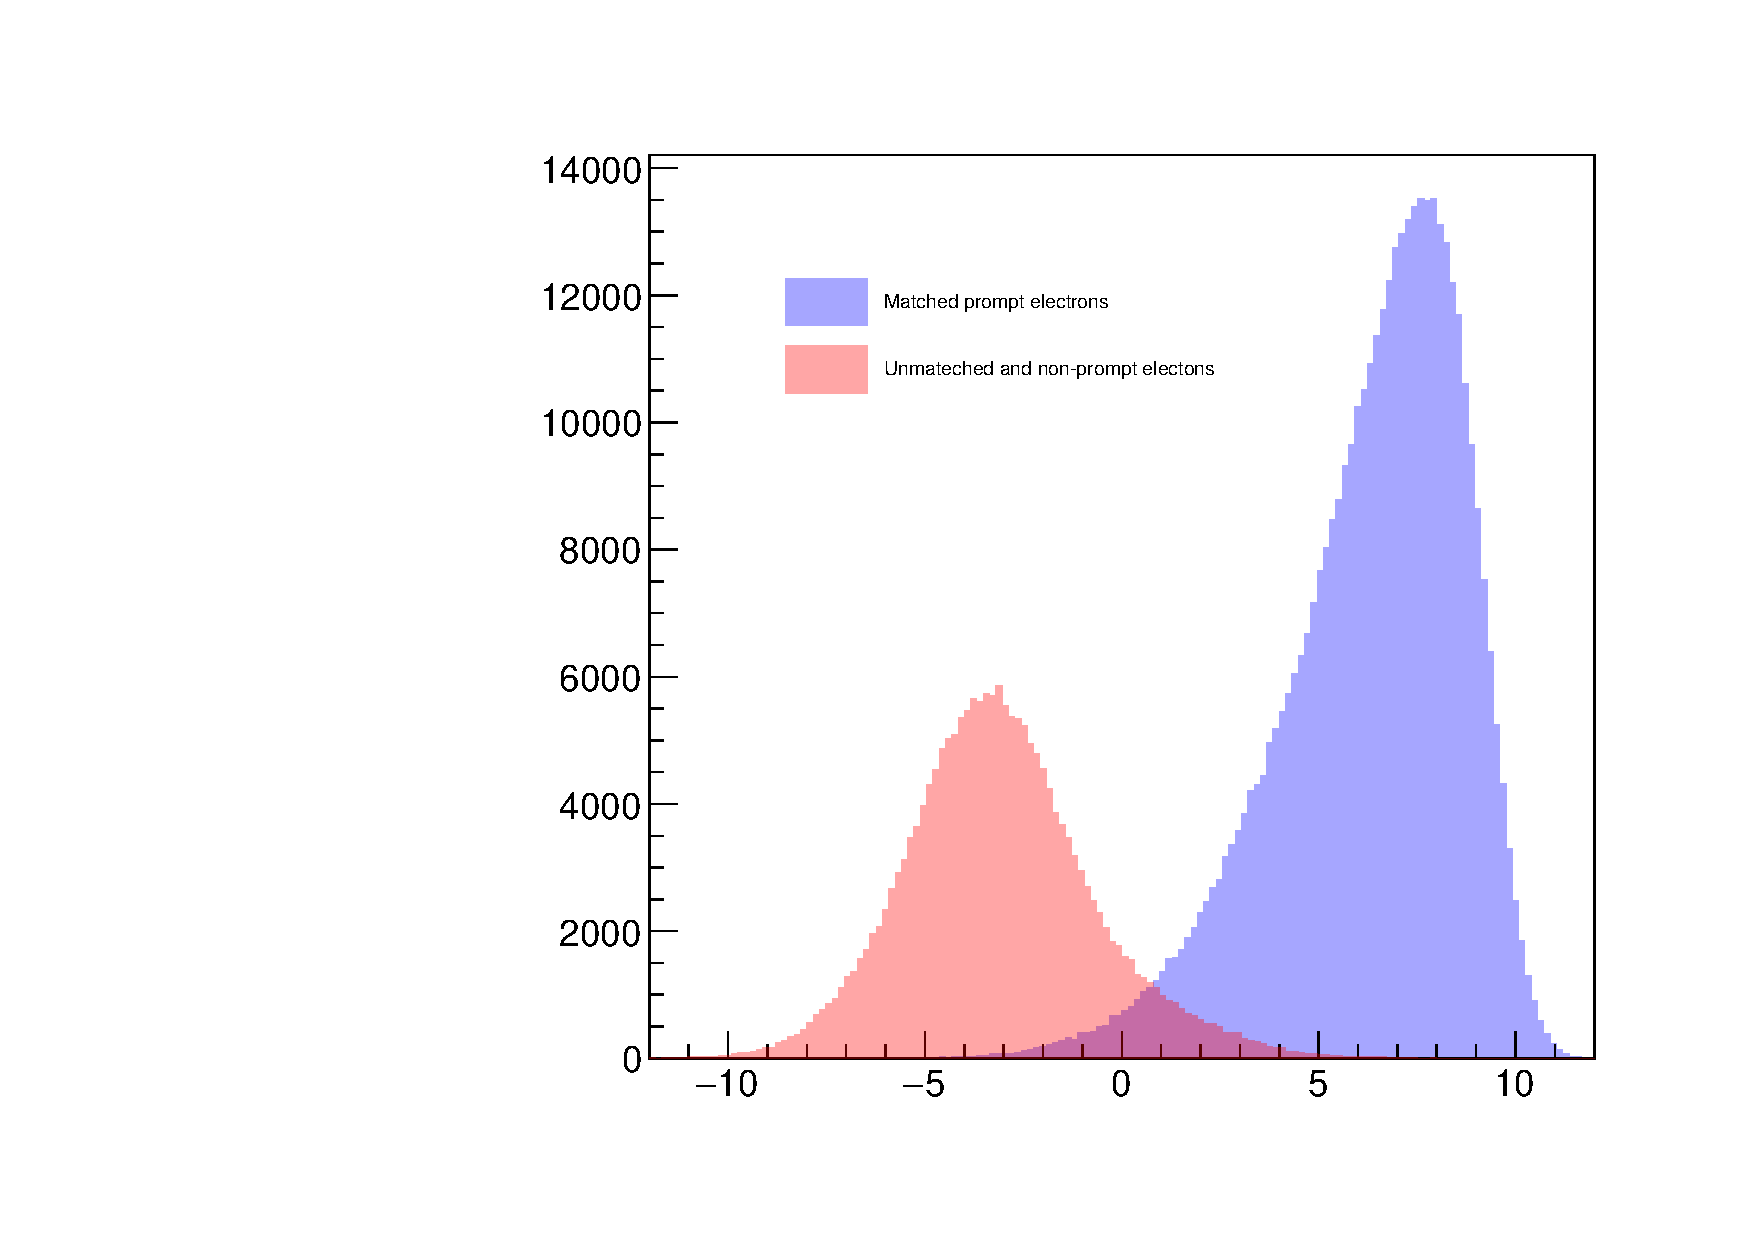
\includegraphics[width=0.80\textwidth]{Figures/Electrons/Ele_BDTv2_Score.pdf}
      \caption{The Output of the multiclassifier discriminant for prompt electrons matched to truth electrons from $Z$ decay (blue) and for misindentified
      electrons (red). Events are all taken from Drell-Yan with jets MC sample.
      \label{fig:ele_MVA_score_2018}}
   \end{center}
\end{figure}

\begin{figure}[!htb]
   \vspace*{0.3cm}
   \begin{center}
      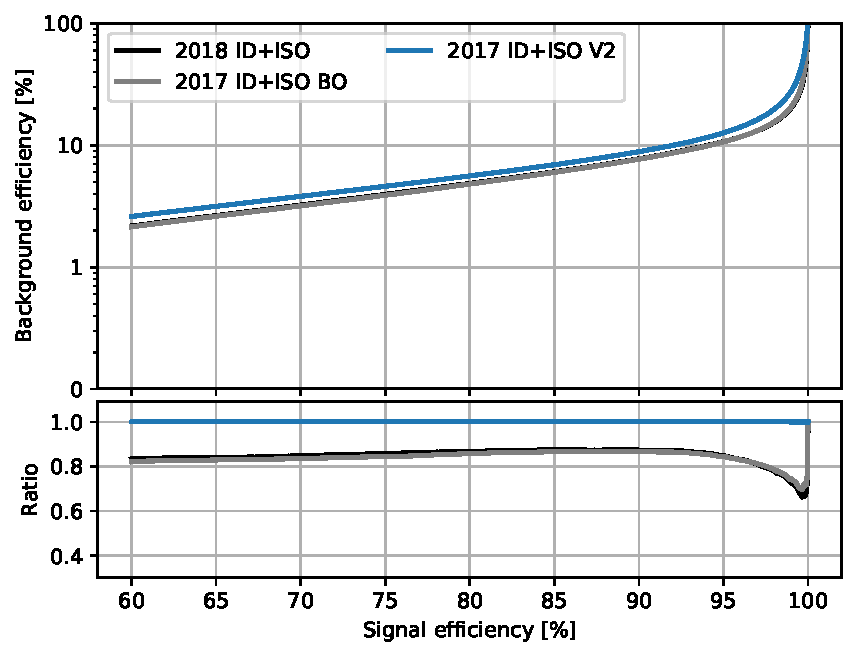
\includegraphics[width=0.45\textwidth]{Figures/Electrons/2018_EB1_5.pdf}
      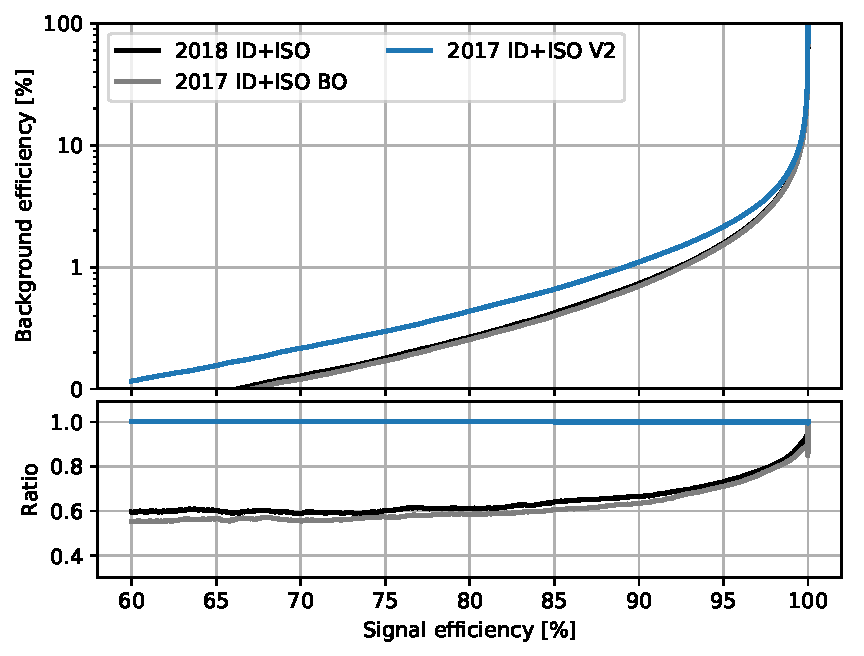
\includegraphics[width=0.45\textwidth]{Figures/Electrons/2018_EB1_10.pdf} \\
      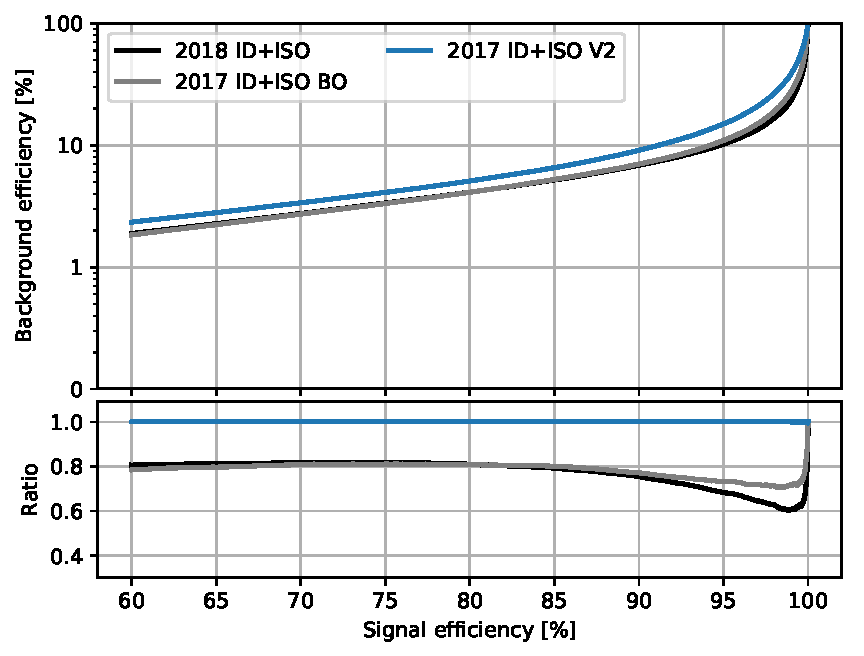
\includegraphics[width=0.45\textwidth]{Figures/Electrons/2018_EB2_5.pdf}
      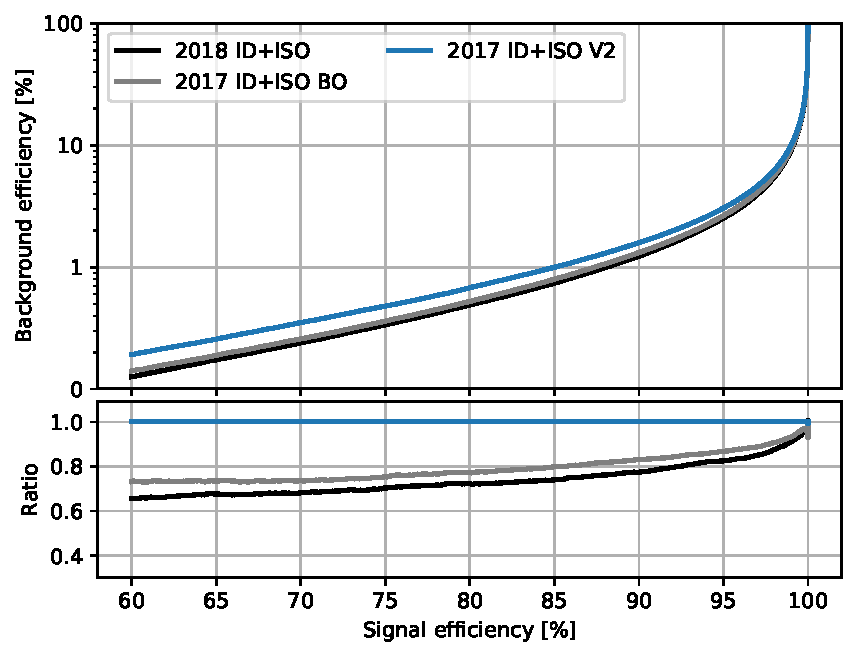
\includegraphics[width=0.45\textwidth]{Figures/Electrons/2018_EB2_10.pdf}\\
      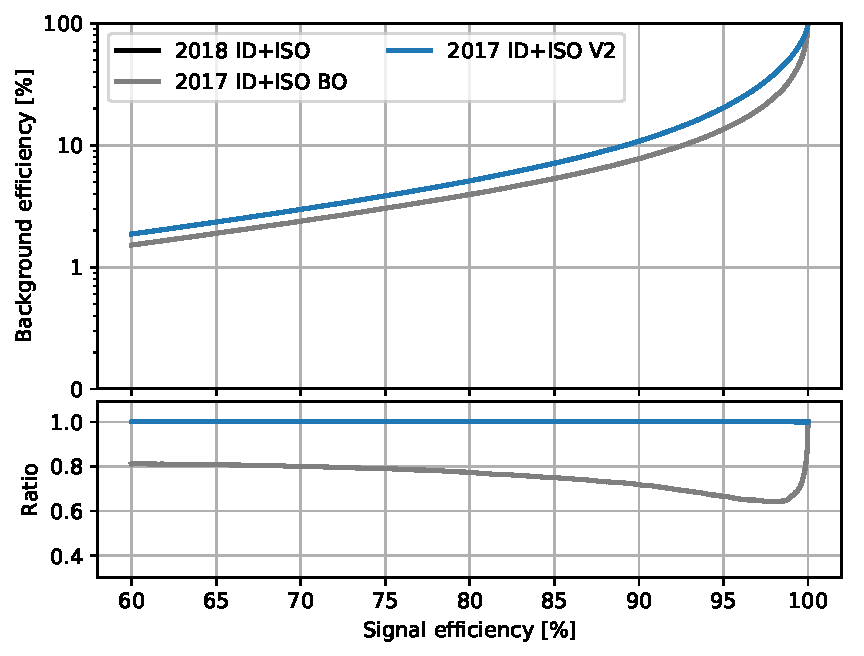
\includegraphics[width=0.45\textwidth]{Figures/Electrons/2018_EE_5.pdf}
      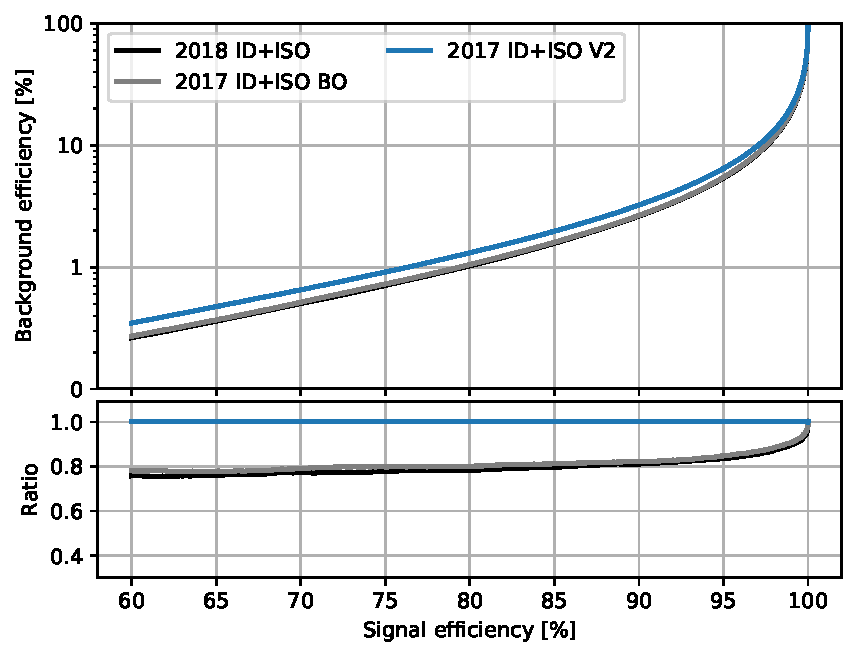
\includegraphics[width=0.45\textwidth]{Figures/Electrons/2018_EE_10.pdf} \\
   \caption{The receiver operating characteristic curves, representing the background efficiency vs signal efficiency, of the MVA trained on the 2017 Drell-Yan
   with jets MC sample and applied on the 2018 Drell-Yan with jets MC sample. The training combines identification and isolation fautures. Performance are shown
   for electrons with $5 < p_T < 10$ GeV (left), $p_T > 10 GeV$ (right), and $|\eta|<0.8$ (top), $0.8 < |\eta| < 1.479$ (middle), and $|\eta| > 1.479$ (bottom).
   V1 and V2 versions of training are compared, exploiting TMVA and xgboost training libraries respectively.
   \label{fig:ele_ID_ISO_ROC_2018}}
   \end{center}
\end{figure}

The impact of the transition from the TMVA (V1) to the XGBoost(V2) training framework is shown in Fig.~\ref{fig:ele_ID_ISO_ROC_V1_vs_V2}, showing a noticeable improvement.
% The working points shown are chosen so as to get the  same signal efficiency as a cut on MVA ID and a cut on the PF isolation, in each $p_T$ and $\eta$ bin.

\begin{figure}[!htb]
   \vspace*{0.3cm}
   \begin{center}
      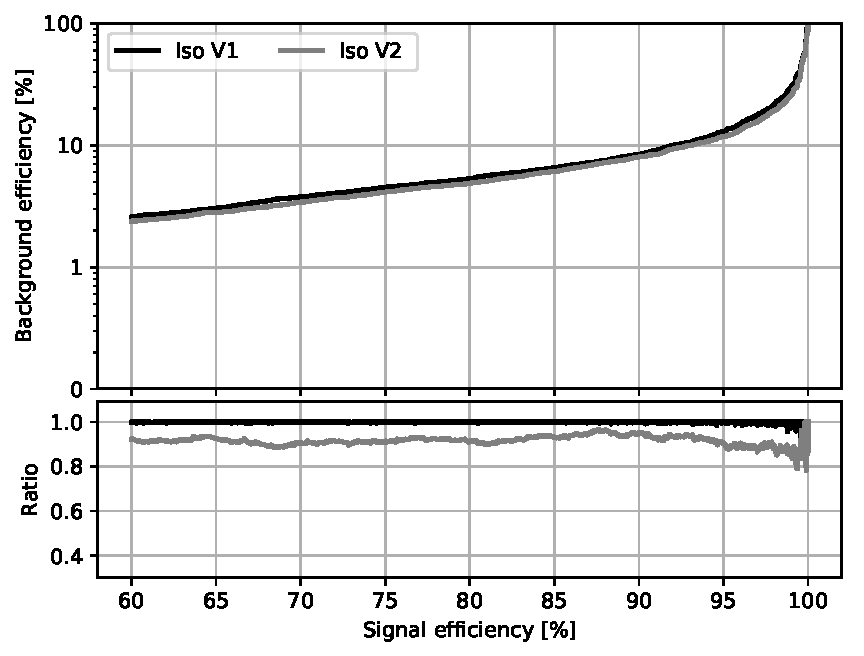
\includegraphics[width=0.45\textwidth]{Figures/Electrons/2018_EB1_5_.pdf}
      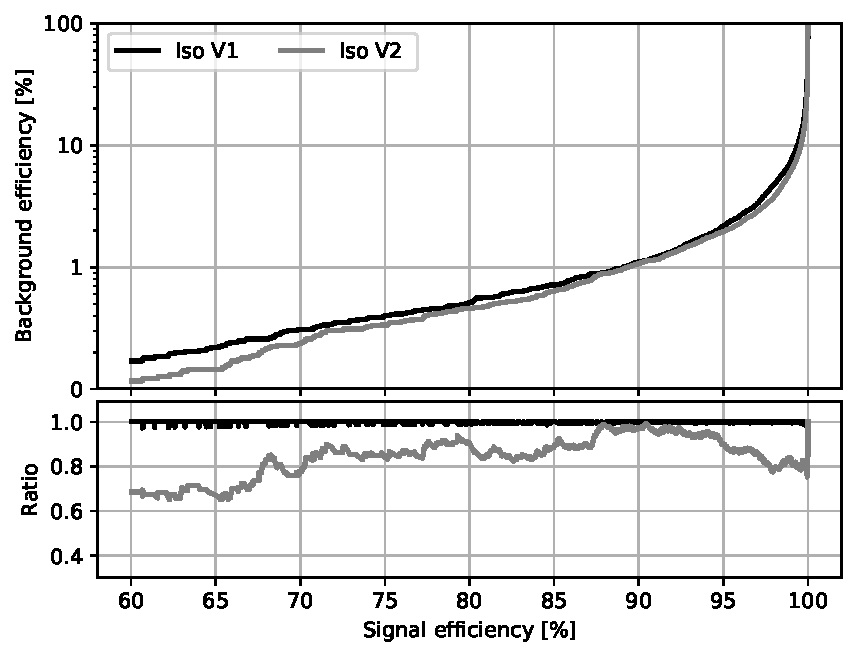
\includegraphics[width=0.45\textwidth]{Figures/Electrons/2018_EB1_10_.pdf} \\
      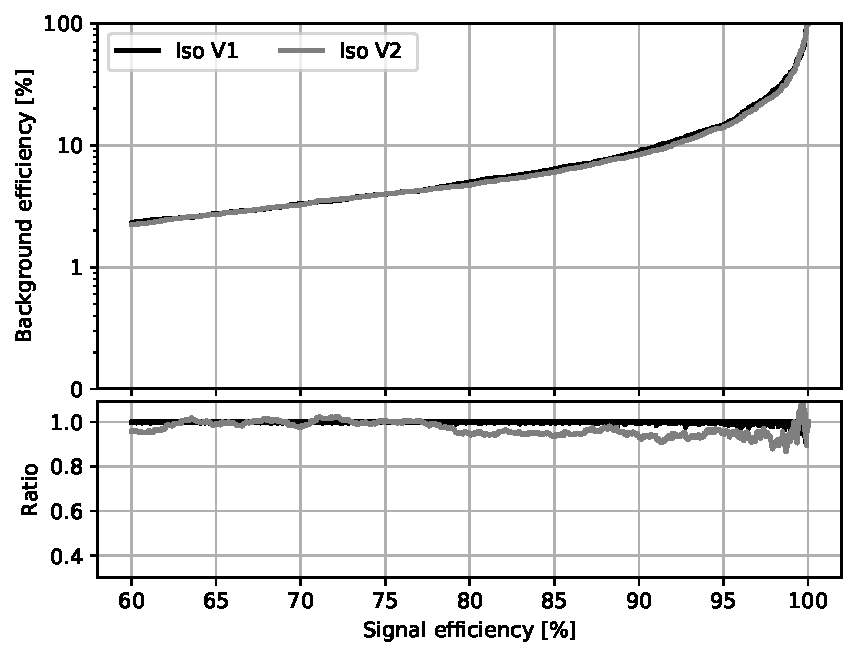
\includegraphics[width=0.45\textwidth]{Figures/Electrons/2018_EB2_5_.pdf}
      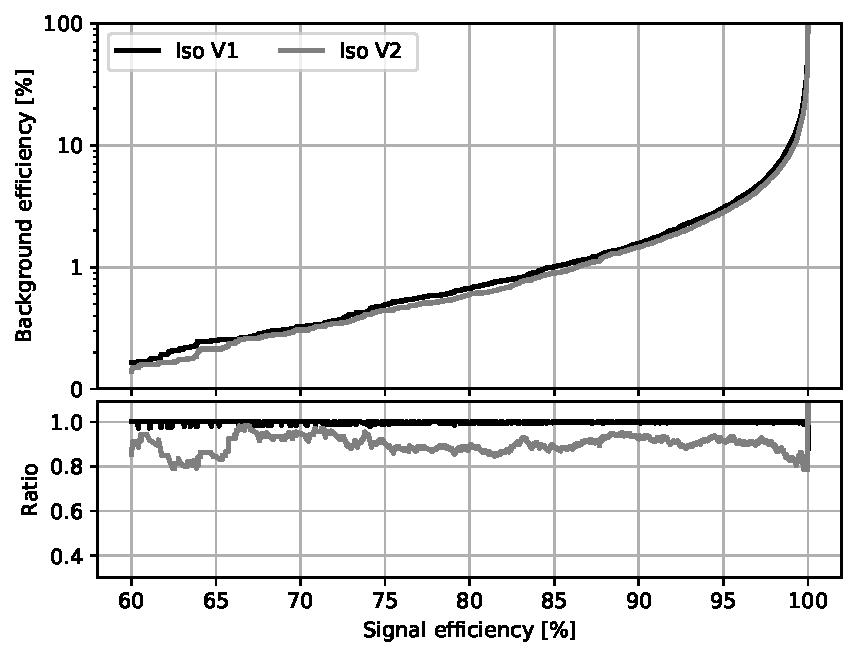
\includegraphics[width=0.45\textwidth]{Figures/Electrons/2018_EB2_10_.pdf} \\
      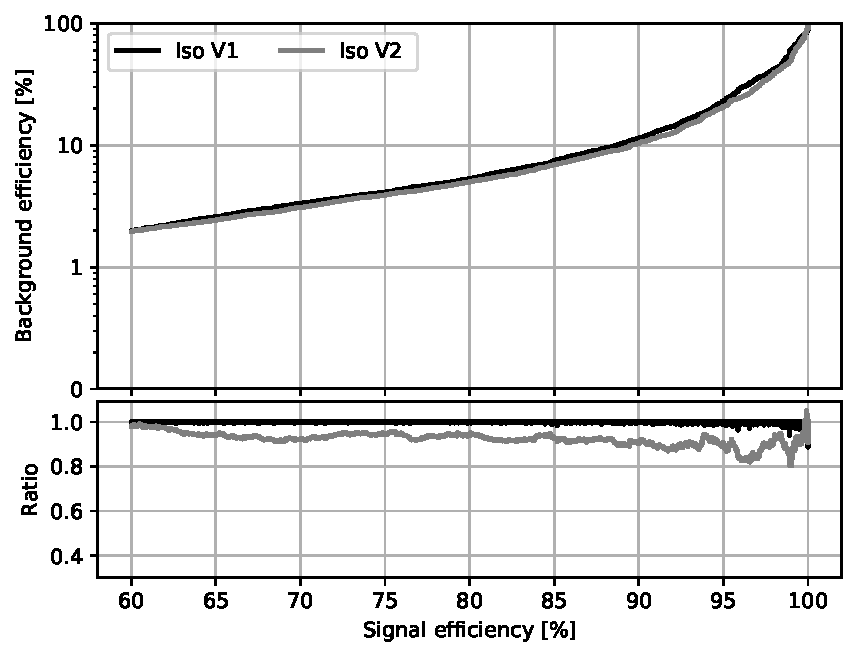
\includegraphics[width=0.45\textwidth]{Figures/Electrons/2018_EE_5_.pdf}
      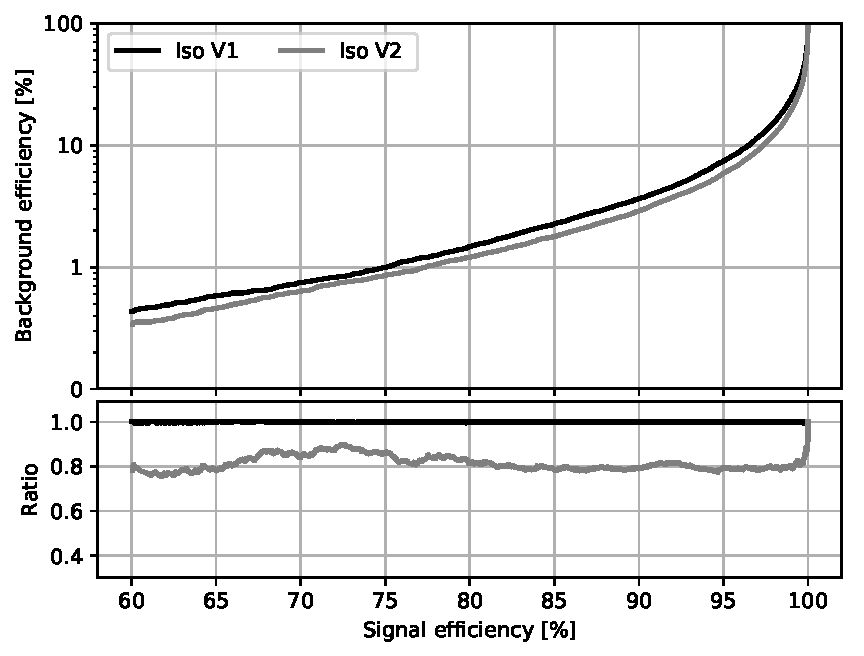
\includegraphics[width=0.45\textwidth]{Figures/Electrons/2018_EE_10_.pdf} \\
   \caption{Performance comparison, background efficiency vs signal efficiency, of the MVA trained using TMVA framework (V1) and XGBoost framework (V2). The
   performance are shown for electrons with $5 < p_T < 10$ GeV (left), $p_T > 10 GeV$ (right), and $|\eta|<0.8$ (top), $0.8 < |\eta| < 1.479$ (middle), and
   $|\eta| > 1.479$ (bottom).
\label{fig:ele_ID_ISO_ROC_V1_vs_V2}}
\end{center}
\end{figure}



% \begin{figure}[!htb]
% \vspace*{0.3cm}
% \begin{center}
% \includegraphics[width=0.5\textwidth]{Figures/Electrons/ele_overtraining.png}
% \caption{BDT output for the training and testing sample for true and fake electrons in the high-$p_T$ endcap training bins.
% \label{fig:ele_ID_BDT_output}}
% \end{center}
% \end{figure}

%Table~\ref{tab:ele_ID_input_variables} summarizes the full list of observables used as input to the classifier
Tables~\ref{tab:ele_ID_WPA},~\ref{tab:ele_ID_WPB} and ~\ref{tab:ele_ID_WPC} list the cuts values applied to the MVA output for 2016, 2017, 2018 training, respectively. For 2018, the corresponding signal and background efficiencies are given as examples.They are very similar for 2016 and 2017. 
%e for the chosen working point. 
For the analysis, loose electrons have to pass this MVA identification and isolation working point.

\begin{table}[h!]
%\scriptsize
    \centering
    \begin{tabular}{c|c c c}
\hline
\multicolumn{4}{|c|}{2016 Datasets}                                                                 \\
\hline %----------------------------------------------------------------------------------------
minimum BDT score    &  $|\eta| < 0.8 $ & $0.8 < |\eta| < 1.479$ 	& $|\eta| > 1.479$      \\
\hline %----------------------------------------------------------------------------------------
$ 5 < p_T < 10 $ GeV &  0.9503      & 0.9461  	& 0.9387		\\
$p_T > 10$ GeV         &  0.3782	& 0.3587		&  -0.5745	\\
\hline %----------------------------------------------------------------------------------------
\hline %----------------------------------------------------------------------------------------
     \end{tabular}
\small
    \caption{Minimum BDT score required for passing the electron identification, for 2016 samples.}% \textbf{FIXME: WP to be defined!}}
    \label{tab:ele_ID_WPA}
\end{table}

\begin{table}[h!]
%\scriptsize
    \centering
    \begin{tabular}{c|c c c}
\hline
\multicolumn{4}{|c|}{2017 Datasets}                                                                 \\
\hline %----------------------------------------------------------------------------------------
minimum BDT score    &  $|\eta| < 0.8 $ & $0.8 < |\eta| < 1.479$ 	& $|\eta| > 1.479$      \\
\hline %----------------------------------------------------------------------------------------
$ 5 < p_T < 10 $ GeV &  0.8521    & 0.8268  	& 0.8694		\\
$p_T > 10$ GeV         &  0.9825    & 0.9692	& 0.7935	\\
\hline %----------------------------------------------------------------------------------------
\hline %----------------------------------------------------------------------------------------
     \end{tabular}
\small
    \caption{Minimum BDT score required for passing the electron identification, for 2017 samples.}% \textbf{FIXME: WP to be defined!}}
    \label{tab:ele_ID_WPB}
\end{table}

%2016
 %= (pt<=10 && ((fSCeta<0.8                  && BDT >  0.95034841889) ||
 %                                 (fSCeta>=0.8 && fSCeta<1.479 && BDT >  0.94606270058) ||
 %                                (fSCeta>=1.479               && BDT >  0.93872558098)))
 %                   || (pt>10  && ((fSCeta<0.8                  && BDT >  0.3782357877) ||
   %                                (fSCeta>=0.8 && fSCeta<1.479 && BDT >  0.35871320305) ||
      %                             (fSCeta>=1.479               && BDT >  -0.57451499543)));

%2017
 %  isBDT         = (pt<=10 && ((fSCeta<0.8                  && BDT >  0.85216885148) ||
   %                                (fSCeta>=0.8 && fSCeta<1.479 && BDT >  0.82684550976) ||
   %                                (fSCeta>=1.479               && BDT >  0.86937630022)))
     %               || (pt>10  && ((fSCeta<0.8                  && BDT >  0.98248928759) ||
    %                               (fSCeta>=0.8 && fSCeta<1.479 && BDT >  0.96919224579) ||
   %                                (fSCeta>=1.479               && BDT >  0.79349796445)));

\begin{table}[h!]
%\scriptsize
    \centering
    \begin{tabular}{|c|c c c}
%\multicolumn{4}{|c|}{Datasets}                                                                 \\
%\hline %----------------------------------------------------------------------------------------
\cline{2-4}
  \multicolumn{1}{ c|}{}             & \multicolumn{3}{|c|}{$|\eta| < 0.8 $}                        \\
\cline{2-4} %----------------------------------------------------------------------------------------
   \multicolumn{1}{c|}{}            & Cut on BDT score & Signal eff. & \multicolumn{1}{c|}{Background eff.}  \\
\hline %----------------------------------------------------------------------------------------
$ 5 < p_T < 10 $ GeV              & 0.8956                        & 81.04\%            &  \multicolumn{1}{c|}{4.4\%}  \\
\hline %----------------------------------------------------------------------------------------
 $p_T > 10$ GeV                     &  0.0424	           	     & 97.1\%		&  \multicolumn{1}{c|}{2.9\%}		\\
\hline %----------------------------------------------------------------------------------------
\cline{2-4}
  \multicolumn{1}{ c|}{}             & \multicolumn{3}{|c|}{$0.8 < |\eta| < 1.479$}                        \\
\cline{2-4} %----------------------------------------------------------------------------------------
   \multicolumn{1}{c|}{}            & Cut on BDT score & Signal eff.      & \multicolumn{1}{c|}{Background eff.}  \\
\hline  %----------------------------------------------------------------------------------------
$ 5 < p_T < 10 $ GeV              & 0.9111                     & 79.3\%           &  \multicolumn{1}{c|}{4.6\%}     \\
\hline %----------------------------------------------------------------------------------------
$p_T > 10$ GeV                      &  0.0047		         & 96.3\%	  &  \multicolumn{1}{c|}{3.6\%}		\\
\hline %----------------------------------------------------------------------------------------

\cline{2-4}
  \multicolumn{1}{ c|}{}             & \multicolumn{3}{|c|}{$|\eta| > 1.479$}                        \\
\cline{2-4} %----------------------------------------------------------------------------------------
   \multicolumn{1}{c|}{}            & Cut on BDT score & Signal eff. & \multicolumn{1}{c|}{Background eff.}  \\
\hline  %----------------------------------------------------------------------------------------
$ 5 < p_T < 10 $ GeV              & 0.9401                     & 72.97\%    &  \multicolumn{1}{c|}{3.6\%}     \\
\hline %----------------------------------------------------------------------------------------
$p_T > 10$ GeV                      & -0.6042		   & 95.7\%      &  \multicolumn{1}{c|}{6.7\%}		\\
\hline %----------------------------------------------------------------------------------------

     \end{tabular}
\small
    \caption{Minimum MVA score required for passing the electron identification, together with the corresponding signal and background efficiencies, for 2018 samples.}
\label{tab:ele_ID_WPC}
\end{table}

\clearpage

%
%\subsubsection{Electron Impact Parameter Selection}
%\label{sec:eleSIP}
% In order to ensure that the leptons are consistent with a common primary vertex we require that they have an associated track with a small impact parameter with respect to the event primary vertex.  
We use the significance of the impact parameter to the event vertex, $  {\rm SIP_{3D}} = \frac{\rm IP}{\sigma_{\rm IP}} $, where ${\rm IP}$ is the lepton impact parameter in three dimensions at the point of closest approach with respect to the primary interaction vertex, and $\sigma_{\rm IP}$ the associated uncertainty.  Hereafter, a "primary lepton" is a lepton satisfying $| {\rm SIP_{3D}} | < 4$.               

%
\subsubsection{Electron Energy Calibrations}
%\textbf{FIXME: ReRecoed data are used but additional e-scale and smearing corrections NOT yet available and thus NOT yet applied}
Referred to \cite{CMS-PAS-HIG-19-001}.
%Electrons in data are corrected for features in ECAL energy scale
%in bins of $\pt$ and $\left| \eta \right|$. Corrections are calculated
%on a $\cPZ \to \Pe\Pe$ sample to align the dielectron 
%mass spectrum in the data to that in the MC, and to
%minimize its width.
%
%The $\cPZ \to \Pe\Pe$ mass resolution in Monte Carlo is made to match
%data by applying a pseudorandom Gaussian smearing to electron energies,
%with Gaussian parameters varying in bins of $\pt$ and $\left| \eta \right|$.
%This has the effect of convoluting the electron energy spectrum with a
%Gaussian.
%
%The electron energy scale is measured in data by fitting a Crystall-ball function to the di-electron mass spectrum around the Z peak in the $Z\rightarrow \Pe \Pe$ control region. The energy scale for the 2016, 2017 and 2018 dataset are shown in Fig.~\ref{fig:ele_energy_scaleA},~\ref{fig:ele_energy_scaleB},~\ref{fig:ele_energy_scaleC} (a), respectively, and decently agrees with the MC with the preliminary corrections released so far by EGAMMA POG. % for Moriond. % even without any corrections available at the moment. 
%
%\begin{figure}[!htb]
%\vspace*{0.3cm}
%\begin{center}
%\subfigure [] {\resizebox{8cm}{!}{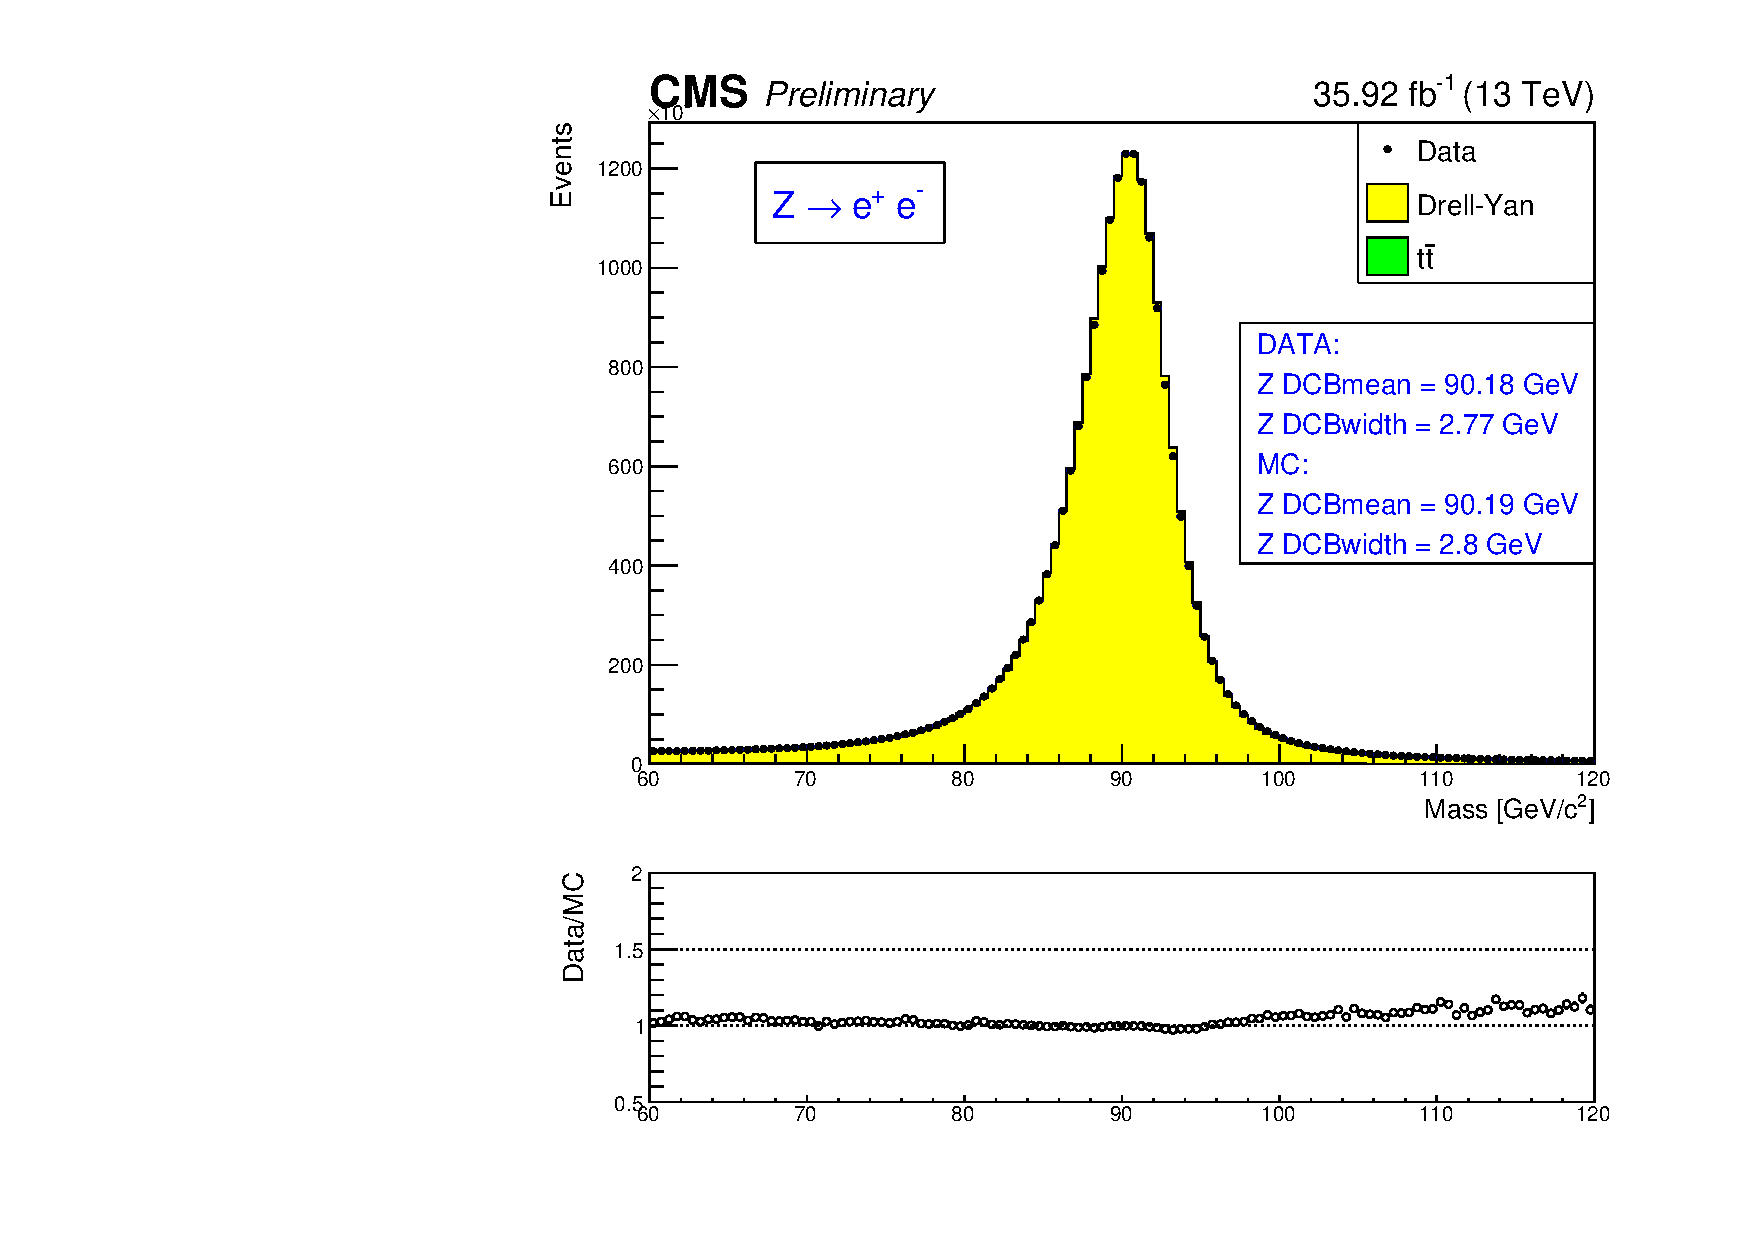
\includegraphics{Figures/Electrons/2016_ZMass_ele.pdf}}}
%\subfigure [] {\resizebox{8cm}{!}{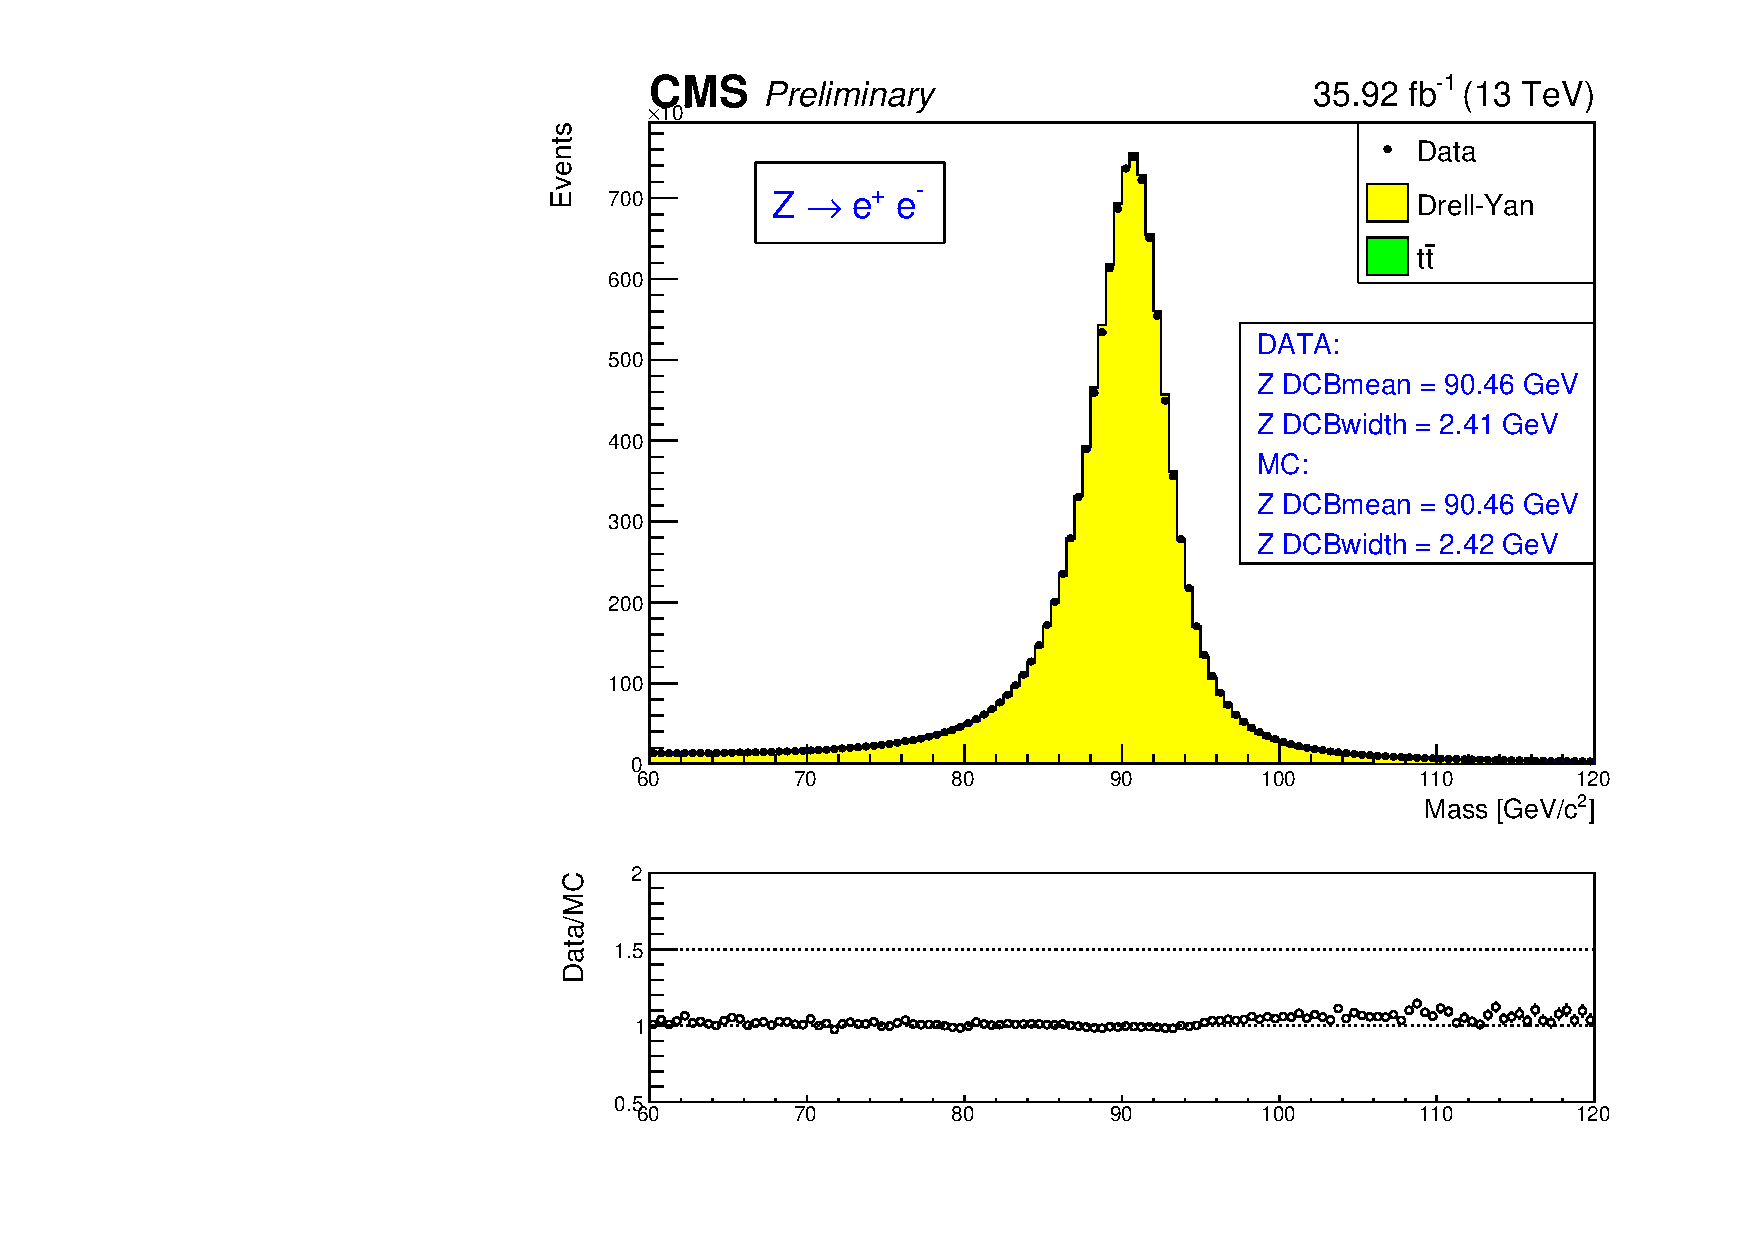
\includegraphics{Figures/Electrons/2016_ZMass_ele_EBEB.pdf}}} \\
%\subfigure [] {\resizebox{8cm}{!}{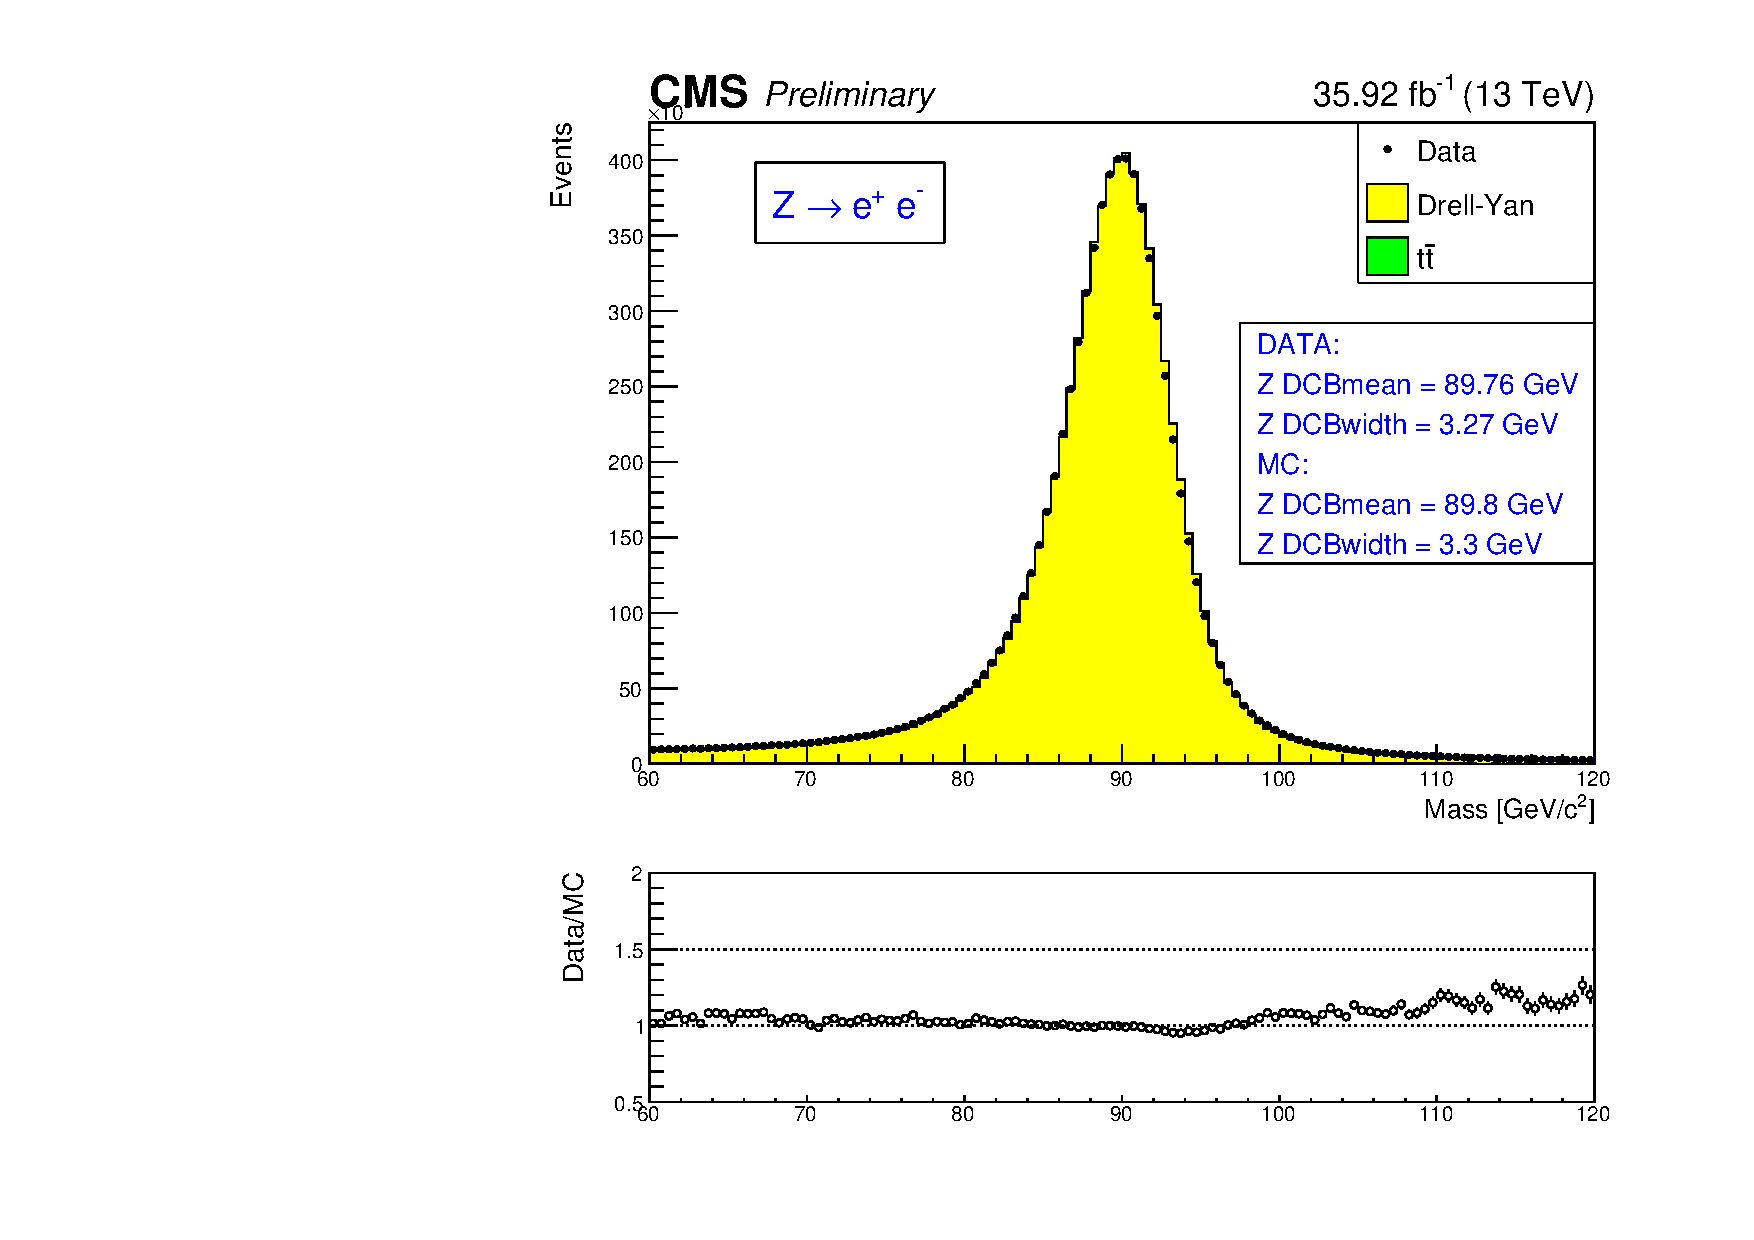
\includegraphics{Figures/Electrons/2016_ZMass_ele_EBEE.pdf}}}
%\subfigure [] {\resizebox{8cm}{!}{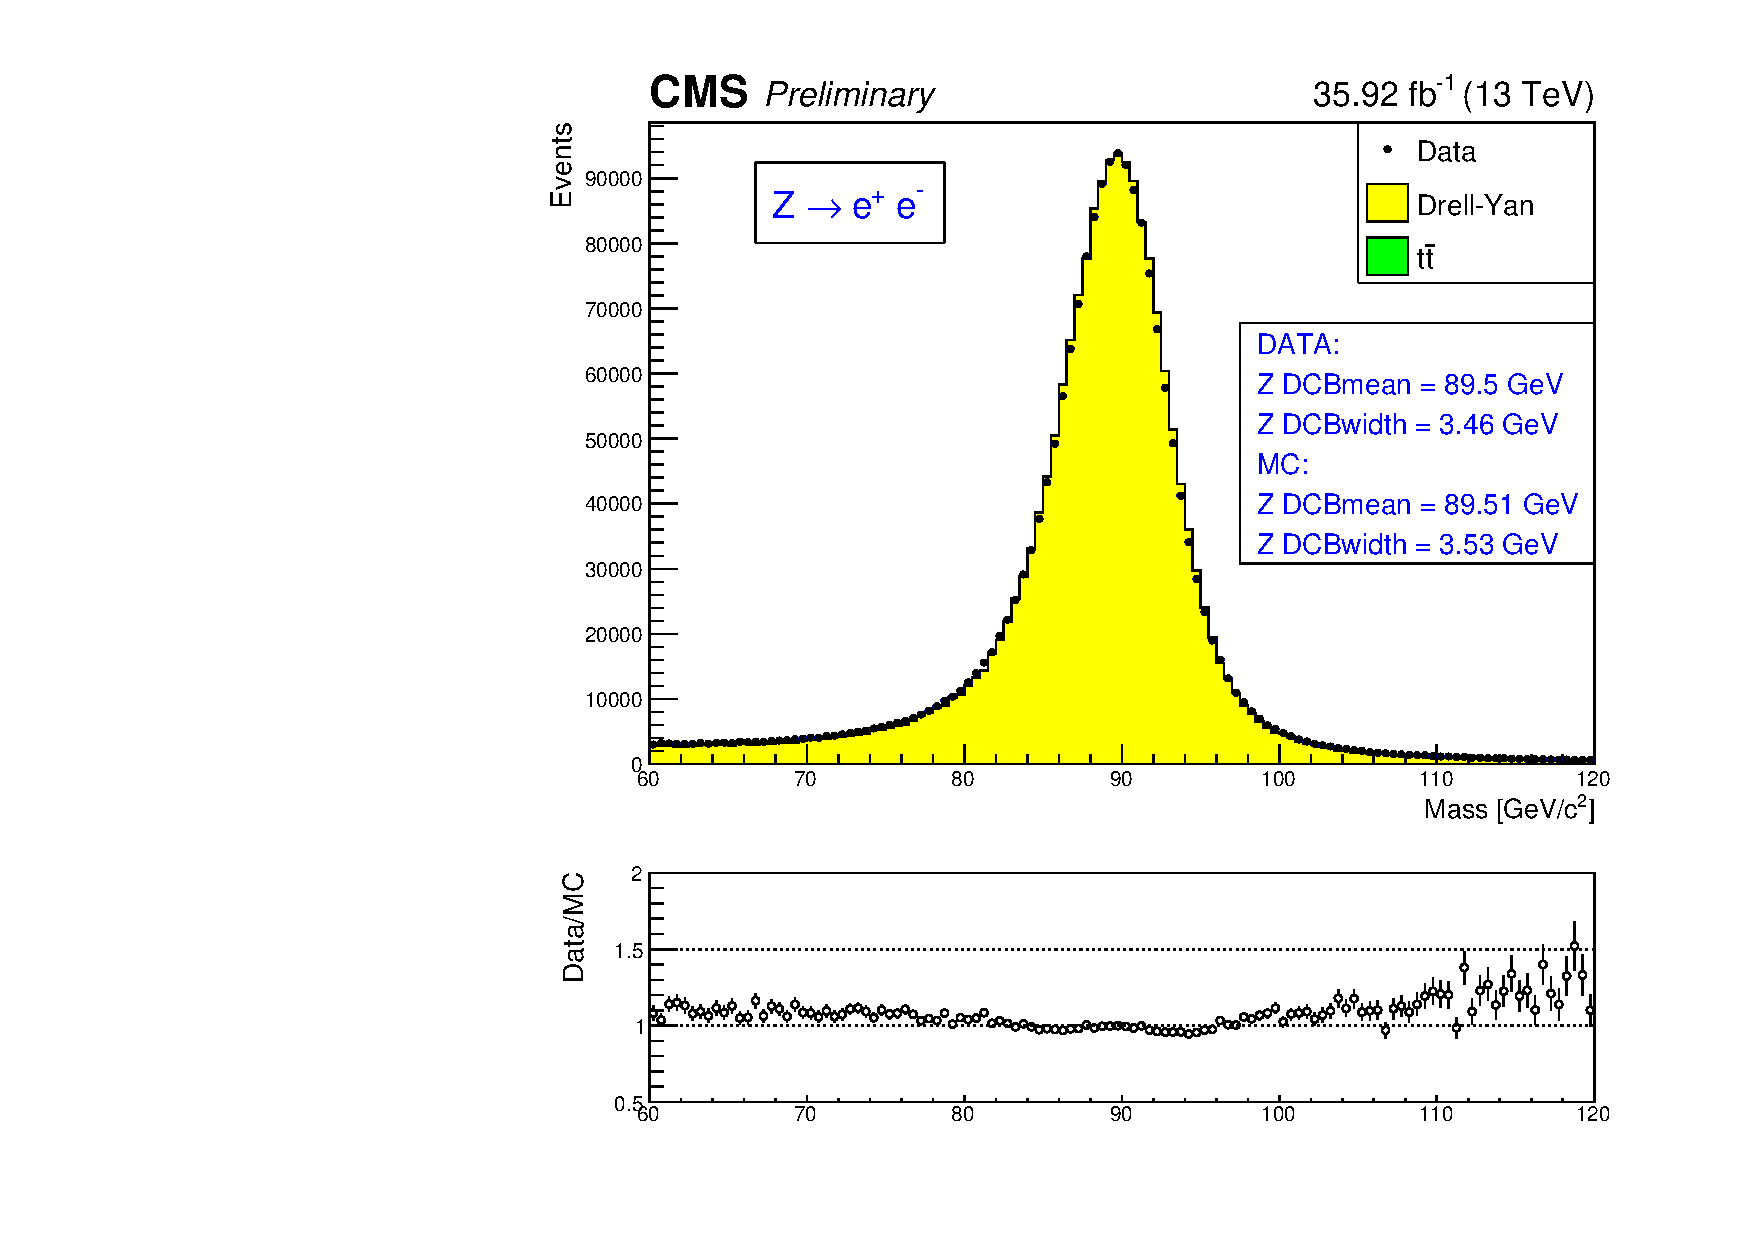
\includegraphics{Figures/Electrons/2016_ZMass_ele_EEEE.pdf}}} \\
%\end{center}
%\caption{
%(a): electron energy scale measured in the $Z\rightarrow \Pe \Pe$ control region for all electrons, for both electrons in the barrel (b), for one electron in the barrel, one in the endcaps (c) and for both electrons in the endcaps (d), for 2016 data.
%The results of the Crystall-ball fit are reported in the figures.
%%\textbf{FIXME: e-scale and smearing corrections NOT yet available and thus NOT yet applied} 
%}
%\label{fig:ele_energy_scaleA}
%\end{figure}
%
%\begin{figure}[!htb]
%\vspace*{0.3cm}
%\begin{center}
%\subfigure [] {\resizebox{8cm}{!}{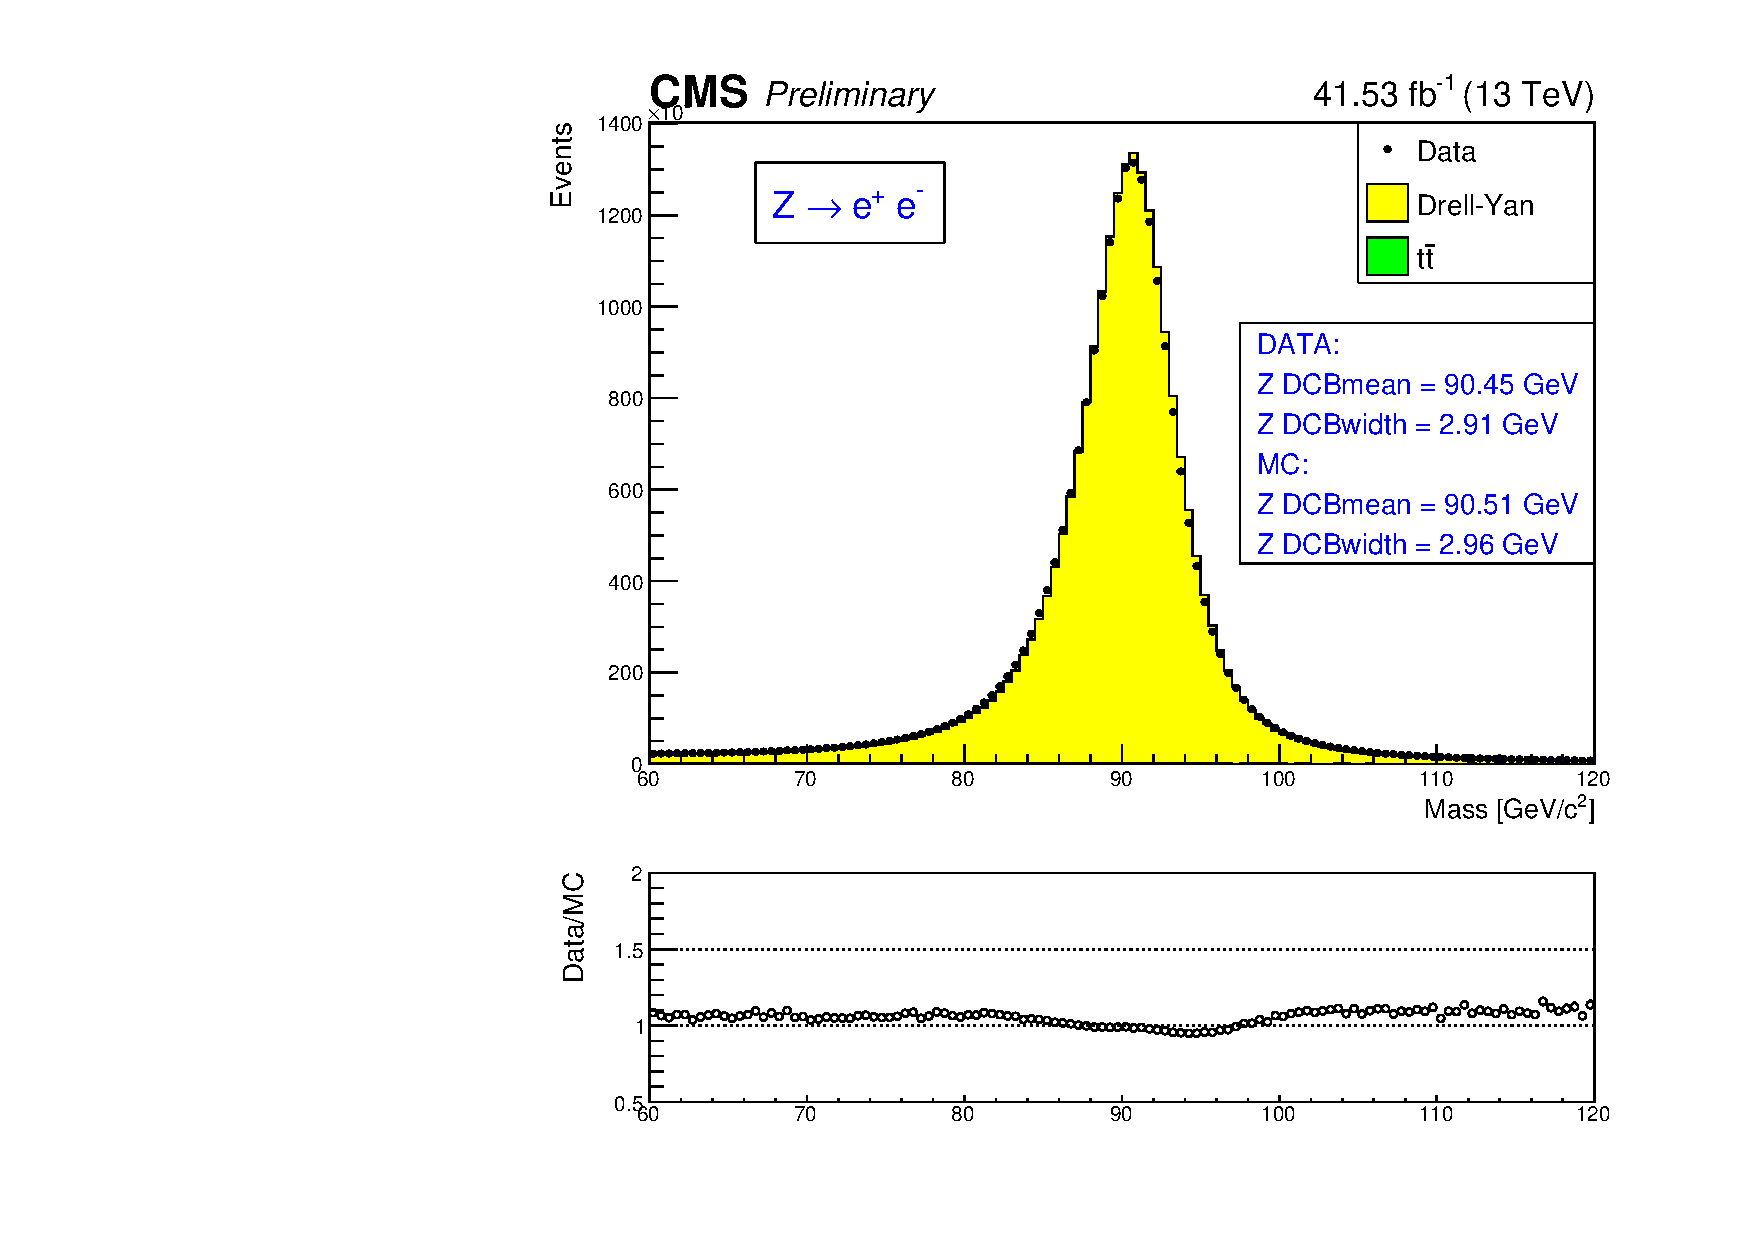
\includegraphics{Figures/Electrons/2017_ZMass_ele.pdf}}}
%\subfigure [] {\resizebox{8cm}{!}{\includegraphics{Figures/Electrons/2017_ZMass_ele_EBEB.pdf}}} \\
%\subfigure [] {\resizebox{8cm}{!}{\includegraphics{Figures/Electrons/2017_ZMass_ele_EBEE.pdf}}}
%\subfigure [] {\resizebox{8cm}{!}{\includegraphics{Figures/Electrons/2017_ZMass_ele_EEEE.pdf}}} \\
%\end{center}
%\caption{
%(a): electron energy scale measured in the $Z\rightarrow \Pe \Pe$ control region for all electrons, for both electrons in the barrel (b), for one electron in the barrel, one in the endcaps (c) and for both electrons in the endcaps (d), for 2017 data.
%The results of the Crystall-ball fit are reported in the figures.
%%\textbf{FIXME: e-scale and smearing corrections NOT yet available and thus NOT yet applied} 
%}
%\label{fig:ele_energy_scaleB}
%\end{figure}
%
%\begin{figure}[!htb]
%\vspace*{0.3cm}
%\begin{center}
%\subfigure [] {\resizebox{8cm}{!}{\includegraphics{Figures/Electrons/2018_ZMass_ele.pdf}}}
%\subfigure [] {\resizebox{8cm}{!}{\includegraphics{Figures/Electrons/2018_ZMass_ele_EBEB.pdf}}} \\
%\subfigure [] {\resizebox{8cm}{!}{\includegraphics{Figures/Electrons/2018_ZMass_ele_EBEE.pdf}}}
%\subfigure [] {\resizebox{8cm}{!}{\includegraphics{Figures/Electrons/2018_ZMass_ele_EEEE.pdf}}} \\
%\end{center}
%\caption{
%(a): electron energy scale measured in the $Z\rightarrow \Pe \Pe$ control region for all electrons, for both electrons in the barrel (b), for one electron in the barrel, one in the endcaps (c) and for both electrons in the endcaps (d), for 2018 data.
%The results of the Crystall-ball fit are reported in the figures. 
%%\textbf{FIXME: e-scale and smearing corrections NOT yet available and thus NOT yet applied} 
%}
%\label{fig:ele_energy_scaleC}
%\end{figure}
%
%\clearpage

%
\subsubsection{Electron Efficiency Measurements}
\label{sec:eleEffMeas}
Referred to \cite{CMS-PAS-HIG-19-001}.

%The Tag-and-Probe study was performed on the EGM dataset using the golden JSON of ~58.83 fb$^{-1}$. More details on the Tag-and-Probe method can be found in Ref.~\cite{AN-15-277}. 
%
%Tag electrons need to satisfy the following quality requirements:
%\begin{itemize}
%%\item trigger matched to HLT\_Ele27\_eta2p1\_WPTight\_Gsf\_v*
%\item~trigger matched to single electron trigger (e.g HLT\_Ele32\_WPTight\_Gsf\_L1DoubleEG\_v* for 2018 for instance)
%\item~$p_{T} > 30$~GeV (tag), super cluster (SC) $\eta < 2.17$% but on in EB-EE gap ($1.4442<|\eta|<1.566$)
%\item~the tag and the probe need to have opposite charge.
%%\item tight working point of the Spring16 cut-based electron ID
%\end{itemize}
%
%For the bin between 7 and 20 GeV, additional criteria are required: 
%\begin{itemize}
%\item~the tag has to pass a cut on the MVA ID$>0.92$, $\sqrt(2*PFMET*p_T(tag)*(1-cos(\phi_{MET}-\phi_{tag})))<45 GeV$.
%\item~tag $p_{T}$ increased to 50 GeV
%\item~the charge is determined with the so-called selection method, asing all three estimates of the electron charge to agree.
%\end{itemize}
%%t
%These additional requirements help cleaning the background and makes the fits more reliable (and thus, the measurement more precise).
%
%Probe electrons only need to be reconstructed as GsfElectron while the FSR recovery algorithm is not applied in efficiency measurement. 
%
%The nominal MC efficiencies are evaluated from the LO MadGraph Drell-Yan, while the NLO systematics use the MadGraph\_AMCatNLO sample (or POWHEG in 2018).
%
%For the efficiency measurements a template fit is used. The $m_{ee}$ signal shape of the passing and failing probes is taken from MC and convoluted with a Gaussian. The data is then fitted with the convoluted MC template and a CMSShape (an Error-function with a one-sided exponential tail). This change follows from the usage of the T\&P tool developed by the EGM POG. For the low $p_T$ bins, a gaussian is added to the signal model for the failing probes. 
%
%%\paragraph{Electron selection efficiency measurements}\mbox{}\\
%%\label{par:Efficiency_measurements}
%
%The electron selection efficiency is measured as a function of the probe electron $p_{T}$ and its SC $\eta$, and separately for electrons falling in the ECAL gaps. Figure \ref{fig:ele_sel_pt_turn_onA},~\ref{fig:ele_sel_pt_turn_onB},~\ref{fig:ele_sel_pt_turn_onC} and~\ref{fig:ele_sel_eta_turn_onA},\ref{fig:ele_sel_eta_turn_onB},~\ref{fig:ele_sel_eta_turn_onC} show the $p_{T}$ and $\eta$ turn-on curves measured in data, for 2016, 2017 and 2018.
%% and the final 2D scale factor is shown in Fig.~\ref{fig:ele_sel_scale_factors} together with the systematic uncertainties. %These scale factors are very similar to the ICHEP figures, but more homogenous across $\eta$ and $p_{T}$ because of the higher statistics and the usage of more stable fitting routines in the new T\&P tool.
%
%%\includegraphics[page=2, width=0.4\textwidth]{Figures/Electrons/ErecoEta}\\
%
%\begin{figure}[!htb]
%\begin{center}
%    \subfigure [] {\resizebox{7.5cm}{!}{\includegraphics[page=1]{Figures/Electrons/2016_egammaEffitxt_egammaPlots.pdf}}} %eleSFvspT.png}}}
%    \subfigure [] {\resizebox{7.5cm}{!}{\includegraphics[page=1]{Figures/Electrons/2016_egammaEffitxt_egammaPlotsGAP.pdf}}} \\
%    %    \subfigure [] {\resizebox{7.5cm}{!}{\includegraphics{Figures/Electrons/eleSFvspTgap.png}}}\\
%\caption{Electron selection efficiencies vs $p_T$ measured using the Tag-and-Probe technique described in the text, non-gap electrons (left) and gap electrons (right), together with the corresponding data/MC ratio (bottom), for 2016 samples.}
%\label{fig:ele_sel_pt_turn_onA}
%\end{center}
%\end{figure}
%
%\begin{figure}[!htb]
%\begin{center}
%    \subfigure [] {\resizebox{7.5cm}{!}{\includegraphics[page=2]{Figures/Electrons/2016_egammaEffitxt_egammaPlots.pdf}}}
%    \subfigure [] {\resizebox{7.5cm}{!}{\includegraphics[page=2]{Figures/Electrons/2016_egammaEffitxt_egammaPlotsGAP.pdf}}}\\
%\caption{Electron selection efficiencies vs $\eta$ measured using the Tag-and-Probe technique described in the text, non-gap electrons (left) and gap electrons (right), together wit the corresponding data/MC ratio at the bottom of each plot, for 2016 samples. Dashed lines is MC, solid lines is DATA.}
%\label{fig:ele_sel_eta_turn_onA}
%\end{center}
%\end{figure}
%
%\begin{figure}[!htb]
%\begin{center}
%    \subfigure [] {\resizebox{7.5cm}{!}{\includegraphics[page=1]{Figures/Electrons/2017_egammaEffitxt_egammaPlots.pdf}}} %eleSFvspT.png}}}
%    \subfigure [] {\resizebox{7.5cm}{!}{\includegraphics[page=1]{Figures/Electrons/2017_egammaEffitxt_egammaPlotsGAP.pdf}}} \\
%    %    \subfigure [] {\resizebox{7.5cm}{!}{\includegraphics{Figures/Electrons/eleSFvspTgap.png}}}\\
%\caption{Electron selection efficiencies vs $p_T$ measured using the Tag-and-Probe technique described in the text, non-gap electrons (left) and gap electrons (right), together with the corresponding data/MC ratio (bottom), for 2017 samples.}
%\label{fig:ele_sel_pt_turn_onB}
%\end{center}
%\end{figure}
%
%\begin{figure}[!htb]
%\begin{center}
%    \subfigure [] {\resizebox{7.5cm}{!}{\includegraphics[page=2]{Figures/Electrons/2017_egammaEffitxt_egammaPlots.pdf}}}
%    \subfigure [] {\resizebox{7.5cm}{!}{\includegraphics[page=2]{Figures/Electrons/2017_egammaEffitxt_egammaPlotsGAP.pdf}}}\\
%\caption{Electron selection efficiencies vs $\eta$ measured using the Tag-and-Probe technique described in the text, non-gap electrons (left) and gap electrons (right), together wit the corresponding data/MC ratio at the bottom of each plot, for 2017 samples. Dashed lines is MC, solid lines is DATA.}
%\label{fig:ele_sel_eta_turn_onB}
%\end{center}
%\end{figure}
%
%\begin{figure}[!htb]
%\begin{center}
%    \subfigure [] {\resizebox{7.5cm}{!}{\includegraphics[page=1]{Figures/Electrons/2018_egammaEffitxt_egammaPlots.pdf}}} %eleSFvspT.png}}}
%    \subfigure [] {\resizebox{7.5cm}{!}{\includegraphics[page=1]{Figures/Electrons/2018_egammaEffitxt_egammaPlotsGAP.pdf}}} \\
%    %    \subfigure [] {\resizebox{7.5cm}{!}{\includegraphics{Figures/Electrons/eleSFvspTgap.png}}}\\
%\caption{Electron selection efficiencies vs $p_T$ measured using the Tag-and-Probe technique described in the text, non-gap electrons (left) and gap electrons (right), together with the corresponding data/MC ratio (bottom), for 2018 samples.}
%\label{fig:ele_sel_pt_turn_onC}
%\end{center}
%\end{figure}
%
%\begin{figure}[!htb]
%\begin{center}
%    \subfigure [] {\resizebox{7.5cm}{!}{\includegraphics[page=2]{Figures/Electrons/2018_egammaEffitxt_egammaPlots.pdf}}}
%    \subfigure [] {\resizebox{7.5cm}{!}{\includegraphics[page=2]{Figures/Electrons/2018_egammaEffitxt_egammaPlotsGAP.pdf}}}\\
%\caption{Electron selection efficiencies vs $\eta$ measured using the Tag-and-Probe technique described in the text, non-gap electrons (left) and gap electrons (right), together wit the corresponding data/MC ratio at the bottom of each plot, for 2018 samples. Dashed lines is MC, solid lines is DATA.}
%\label{fig:ele_sel_eta_turn_onC}
%\end{center}
%\end{figure}
%
%%\begin{figure}[!htb]
%%\begin{center}
%%    \subfigure [] {\resizebox{7.5cm}{!}{\includegraphics{Figures/Placeholder.png}}}
%%    \subfigure [] {\resizebox{7.5cm}{!}{\includegraphics{Figures/Placeholder.png}}}\\
%%\caption{2D ($p_T, \eta$) Electron selection Scale Factors measured using the Tag-and-Probe technique described in the text, non-gap electrons (left) and gap electrons (right).}
%%\label{fig:ele_sel_scale_factors}
%%\end{center}
%%\end{figure}
%
%
%%\paragraph{Systematic uncertainties}\mbox{}\\
%%\label{par:Systematic_uncertainties}
%%%%%%%%%%%%%%%%%%%%%%%%%%%%%
%
% The EGM recommendations on the evaluation of Tag-and-Probe uncertainties for efficiency measurements are followed. Specifically, we consider
%
%\begin{itemize}
%   \item Variation of the signal shape from a MC shape to an analytic shape (Crystal Ball) fitted to the MC
%   \item Variation of the background shape from a CMS-shape to a simple exponential in fits to data
%%   \item Variation of the tag selection: tag $p_{T}>$35~GeV and passes MVA-based 8X ID
%   \item Using an NLO MC sample for the signal templates
%\end{itemize}
%
%The total uncertainty for the measurement of the scale factors is the quadratic sum of the statistical uncertainties returned from the fit and the aforementioned systematic uncertainties.
%
%\clearpage
%
%
%

%
%\clearpage
%
\subsection{Muons}
%
%\subsubsection{Muon Reconstruction}
\subsubsection{Muon Reconstruction and Identification}
\label{sec:muonReco}
Referred to \cite{CMS-PAS-HIG-19-001}.
%
%More details on muon reconstruction can be found in Ref.~\cite{AN-15-277}.
%We define {\bf loose muons} as the muons that satisfy  
%$p_T > 5$, $|\eta| < 2.4$, $dxy< 0.5$ cm, $dz < 1$ cm, where $dxy$ and $dz$ are 
%defined w.r.t. the PV and using the 'muonBestTrack'. Muons have to be 
%reconstructed by either the Global Muon or Tracker Muon algorithm. Standalone 
%Muon tracks that are only reconstructed in the muon system are rejected.
%Muons with \verb|muonBestTrackType==2| (standalone) are discarded even if they 
%are marked as global or tracker muons. 
%
%Loose muons with $\pt$ below 200\GeV are considered identified muons if they 
%also pass 
%%Muon BDT (see below).
%the PF muon ID (note that the naming 
%convention used for these IDs differs from the muon POG naming scheme, in which the ``tight ID'' used here is called the ``loose ID''). 
%Loose muons with $\pt$  above 200\GeV are considered identified muons if they pass the PF ID or the Tracker
%High-$\pt$ ID, the definition of which is shown in Table~\ref{tab:highPtID}.
%This relaxed definition is used to increase signal efficiency for the high-mass
%search. When a very heavy resonance decays to two $\cPZ$ bosons, both bosons
%will be very boosted. In the lab frame, the leptons coming from the decay of
%a highly boosted $\cPZ$ will be nearly collinear, and the PF ID loses 
%efficiency for muons separated by approximately $\Delta R < 0.4$, which roughly 
%corresponds to muons originating from $\cPZ$ bosons with $\pt > 500\GeV$.
%
%\begin{table}[h]
%    \begin{small}
%    \begin{center}
%    \caption{
%      The requirements for a muon to pass the Tracker High-$\pt$ ID. Note that
%      these are equivalent to the Muon POG High-$\pt$ ID with the global track 
%      requirements removed.
%      }
%    \begin{tabular}{|l|l|}
%      \hline
%      Plain-text description         & Technical description                 \\
%      \hline
%      Muon station matching          & Muon is matched to segments           \\
%                                     & in at least two muon stations         \\
%                                     & \textbf{NB: this implies the muon is} \\
%                                     & \textbf{an arbitrated tracker muon.}  \\
%      \hline                                                          
%      Good $\pt$ measurement         & $\frac{\pt}{\sigma_{\pt}} < 0.3$      \\
%      \hline
%      Vertex compatibility ($x-y$)   & $d_{xy} < 2$~mm                       \\
%      \hline
%      Vertex compatibility ($z$)     & $d_{z} < 5$~mm                        \\
%      \hline
%      Pixel hits                     & At least one pixel hit                \\
%      \hline
%      Tracker hits                   & Hits in at least six tracker layers   \\
%      \hline
%    \end{tabular}
%    \label{tab:highPtID}
%    \end{center}
%    \end{small}
%\end{table}
%
%An additional ``ghost-cleaning'' step is performed to deal with situations when a single muon
%can be incorrectly reconstructed as two or more muons:
%
%\begin{itemize}
%
%\item Tracker Muons that are not Global Muons are required to be arbitrated.
%\item If two muons are sharing 50\% or more of their segments then the muon with lower quality is removed.
%
%\end{itemize}

%
%%\subsubsection{Muon Identification, Isolation, and Impact Parameter Selection}
%%\label{sec:muon_MVA}
%%The main sources of non-prompt muons are non-isolated muons coming from decays of heavy-flavour mesons and mis-reconstructed jets usually originating from
light-flavour quarks. One of the main improvements brought in the analysis is development of new XGBoost multivariate discriminant for muon selection in all
Run 2 data taking periods.

Reconstructed muons are now fully identified by means of an e\textbf{X}treme \textbf{G}radient \textbf{Boost}ing (XGBoost) gradient boosting library already
used to identify electrons. This machine learning framework exploits observables based exclusively on tracking, information from the muon part of the detector
as well as different components of the isolation. The full list of used features can be found in the Table~\ref{tab:muon_MVA_input_variables}.

\begin{table}[H]
\scriptsize
   \centering
   \begin{tabular}{c|l}
\hline
\hline
Observable type & Observable name \\
\hline
\multirow{1}{*}{Kinematic variables}
	& Pseudorapidity $\eta$ \\
\hline
\multirow{2}{*}{Global track quality variables}
	& Global number of valid muon hits\\
	& Normalized Chi2 \\
\hline
\multirow{5}{*}{Track quality variables}
   & Number of valid hits \\
   & Number of valid pixel hits \\
   & SIP3D \\
   & $d_z$ \\
   & $d_{xy}$ \\
\hline
\multirow{3}{*}{Isolation variables}
   & Particle Flow photon isolation sum \\
   & Particle Flow charged hadrons isolation sum \\
   & Particle Flow neutral hadrons isolation sum \\
\hline
\multirow{1}{*}{For PU-resilience}
   & Mean energy density in the event: $\rho$ $(\mathord{\cdot})$ \\
\hline
\hline
     \end{tabular}
\small
    \caption{Overview of input features passed to the identification classifier.}
    \label{tab:muon_MVA_input_variables}
\end{table}

The muons are preselected by requiring $p_T > 5$, $|\eta| < 2.4$, $dxy< 0.5$ cm, $dz < 1$ cm, where $dxy$ and $dz$. Additionally, muons have to be reconstructed
by either the Global Muon or Tracker Muon algorithm. The signal consists of prompt muons matched to truth muons while background is composed of unmatched and true
but non-prompt muons. The MVA models are trained on 2016, 2017, and 2018 Drell-Yan with jets MC sample for both signal and background. The dedicated training for
each of the Run 2 three data taking periods guarantees optimal performance. The simulated samples used to train the model are listed bellow.

\begin{itemize}
\item \textbf{2016} \begin{verbatim}/DYJetsToLL_M-50_TuneCUETP8M1_13TeV-amcatnloFXFX-pythia8/RunIISummer16MiniAODv2-PUMoriond17_80X_mcRun2_asymptotic_2016_TrancheIV_v6_ext2-v1/MINIAODSIM\end{verbatim}
\item \textbf{2017} \begin{verbatim}/DYJetsToLL_M-50_TuneCP5_13TeV-amcatnloFXFX-pythia8/RunIIFall17MiniAOD-94X_mc2017_realistic_v10-v1/MINIAODSIM\end{verbatim}
\item \textbf{2018} \begin{verbatim}/DYJetsToLL_M-50_TuneCP5_13TeV-amcatnloFXFX-pythia8/RunIISpring18MiniAOD-100X_upgrade2018_realistic_v10-v1/MINIAODSIM\end{verbatim}
\end{itemize}

Some distributions of variables used in the training are shown in Fig.~\ref{fig:mu_features_2016}.

\begin{figure}[!htb]
   \vspace*{0.3cm}
   \begin{center}
      \includegraphics[width=0.45\textwidth]{Figures/Muons/mu_eta_5.pdf}
      \includegraphics[width=0.45\textwidth]{Figures/Muons/mu_eta_10.pdf} \\
      \includegraphics[width=0.45\textwidth]{Figures/Muons/mu_chi_square_5.pdf}
      \includegraphics[width=0.45\textwidth]{Figures/Muons/mu_chi_square_10.pdf} \\
      \includegraphics[width=0.45\textwidth]{Figures/Muons/mu_pf_photon_iso_5.pdf}
      \includegraphics[width=0.45\textwidth]{Figures/Muons/mu_pf_photon_iso_10.pdf} \\
      \includegraphics[width=0.45\textwidth]{Figures/Muons/mu_N_pixel_hits_5.pdf}
      \includegraphics[width=0.45\textwidth]{Figures/Muons/mu_N_pixel_hits_10.pdf} \\
   \caption{Distributions of some features used as the input for the MVA training on 2016 Drell-Yan with jets MC sample. Distributions are shown for muons with
   $5 < p_T < 10 $ GeV (left) and $p_T > 10$ GeV (right).}
   \label{fig:mu_features_2016}}
   \end{center}
\end{figure}

The working point (WP) is choosen as follows: yields of 3 main processes in the signal region are calculated using different WPs for different Muon MVA signal
efficiencies:

\begin{itemize}
   \item Low $p_T$ scanned in steps of 5\% (75\% - 95\%), high $p_T$ in steps of 1\% (95\% - 99\%).
   \item Our previous PF muon ID + RelPFiso + SIP3D efficiency was 75\% - 95\%.
   \item Z+X estimated using SS method only with recalculated Fake Rates for each WP.
   \item Plot $S/\sqrt(S+B)$ in search for the optimal WP choice.
\end{itemize}

The MVA score distribution together with the Working Point choice is shown in the Fig.~\ref{fig:mu_MVA_score_2016} for 2016, Fig.~\ref{fig:mu_MVA_score_2017}
for 2017, and Fig.~\ref{fig:mu_MVA_score_2018} for 2018 data taking periods.

\begin{figure}[!htb]
   \vspace*{0.3cm}
   \begin{center}
      \includegraphics[width=0.95\textwidth]{Figures/Muons/MVA_score_5_2016.pdf}\\
      \includegraphics[width=0.95\textwidth]{Figures/Muons/MVA_score_10_2016.pdf}
   \caption{The MVA score and Working Point choice for the MVA trained on 2016 Drell-Yan with jets MC sample. The MVA score is shown for muons with
   $5 < p_T < 10 $ GeV (top) and $p_T > 10$ GeV (bottom).}
   \label{fig:mu_MVA_score_2017}
   \end{center}
\end{figure}

\begin{figure}[!htb]
   \vspace*{0.3cm}
   \begin{center}
      \includegraphics[width=0.95\textwidth]{Figures/Muons/MVA_score_5_2017.pdf}\\
      \includegraphics[width=0.95\textwidth]{Figures/Muons/MVA_score_10_2017.pdf}
   \caption{The MVA score and Working Point choice for the MVA trained on 2017 Drell-Yan with jets MC sample. The MVA score is shown for muons with
   $5 < p_T < 10 $ GeV (top) and $p_T > 10$ GeV (bottom).}
   \label{fig:mu_MVA_score_2017}
   \end{center}
\end{figure}

\begin{figure}[!htb]
   \vspace*{0.3cm}
   \begin{center}
      \includegraphics[width=0.95\textwidth]{Figures/Muons/MVA_score_5_2018.pdf}\\
      \includegraphics[width=0.95\textwidth]{Figures/Muons/MVA_score_10_2018.pdf}
   \caption{The MVA score and Working Point choice for the MVA trained on 2018 Drell-Yan with jets MC sample. The MVA score is shown for muons with
   $5 < p_T < 10 $ GeV (top) and $p_T > 10$ GeV (bottom).}
   \label{fig:mu_MVA_score_2018}
   \end{center}
\end{figure}


In Figs.~\ref{fig:mu_ID_ISO_SIP_ROC} one can compare ROC curve for the model trained on 2016, 2017, and 2018 MC using muon identification, isolation, and impact
parameter features with the sequential PF muon ID $+$ RelPFiso $< 0.35 +$ SIP3D $< 4$ approach marked with dot. Please note that for the comparison reasons the dot has
been moved below the ROC curve in the ration plot so one can easily read the improvement in percentage. As expected, the MVA based approach outperforms the sequential
approach in all data taking periods.

\begin{figure}[!htb]
   \vspace*{0.3cm}
   \begin{center}
      \includegraphics[width=0.45\textwidth]{Figures/Muons/2016_pT_5.pdf}
      \includegraphics[width=0.45\textwidth]{Figures/Muons/2016_pT_10.pdf} \\
      \includegraphics[width=0.45\textwidth]{Figures/Muons/2017_pT_5.pdf}
      \includegraphics[width=0.45\textwidth]{Figures/Muons/2017_pT_10.pdf} \\
      \includegraphics[width=0.45\textwidth]{Figures/Muons/2018_pT_5.pdf}
      \includegraphics[width=0.45\textwidth]{Figures/Muons/2018_pT_10.pdf} \\
   \caption{The receiver operating characteristic curves, representing the background efficiency vs signal efficiency, of the MVA trained on 2016 (top), 2017
   (middle), and 2018 (bottom) Drell-Yan with jets MC sample. Performance are shown for muons with $5 < p_T < 10 $ GeV (left) and $p_T > 10$ GeV (right) The dot
   represents prevoously used sequential PF muon ID $+$ RelPFiso $< 0.35 +$ SIP3D $< 4$ approach.
   \label{fig:mu_ID_ISO_SIP_ROC}}
   \end{center}
\end{figure}


% Several studies have been conducted on 2016 Drell-Yan with jets MC sample. The XGBoost framework was first used in 2017 and the model was trained on 2017
% Drell-Yan with jets MC sample. This model is known as 2017 ID+ISO V2. The same framework was then used to train the model on 2016 MC (2016 ID+ISO) and finally
% on 2018 MC (2018 ID+ISO). In Fig.~\ref{fig:ele_ID_ISO_ROC_2016} one can see the ROC curves obtained using 2016 Drell-Yan with jets MC sample. As expected, the
% model trained on 2016 MC using electron identification and isolation features outperforms the model trained on 2016 MC using only identification features and
% the model obtained after applying 2017 ID+ISO V2 training on 2016 Drell-Yan with jets MC sample.
%
% In Fig.~\ref{fig:ele_ID_ISO_ROC_2016_} one can see the ROC curve for the model trained on 2016 MC using electron identification and isolation features and ROC
% curve when applying sequential approach meaning applying isolation cut after cutting on the distribution obtained by training using only identification features.
% As expected, the model obtained using electron identification and isolation features outperforms the sequential approach model.
%
% \begin{figure}[!htb]
%    \vspace*{0.3cm}
%    \begin{center}
%       \includegraphics[width=0.45\textwidth]{Figures/Electrons/2016_EB1_5.pdf}
%       \includegraphics[width=0.45\textwidth]{Figures/Electrons/2016_EB1_10.pdf} \\
%       \includegraphics[width=0.45\textwidth]{Figures/Electrons/2016_EB2_5.pdf}
%       \includegraphics[width=0.45\textwidth]{Figures/Electrons/2016_EB2_10.pdf} \\
%       \includegraphics[width=0.45\textwidth]{Figures/Electrons/2016_EE_5.pdf}
%       \includegraphics[width=0.45\textwidth]{Figures/Electrons/2016_EE_10.pdf} \\
%    \caption{The receiver operating characteristic curves, representing the background efficiency vs signal efficiency, of the MVA trained on 2016 Drell-Yan with
%    jets MC sample. Performance are shown for electrons with $5 < p_T < 10 $ GeV (left), $p_T > 10$ GeV (right), and $|\eta| < 0.8$ (top),
%    $0.8 < |\eta| < 1.479$ (middle), and $|\eta| > 1.479$ (bottom).
%    \label{fig:ele_ID_ISO_ROC_2016}}
%    \end{center}
% \end{figure}
%
%
% \begin{figure}[!htb]
%    \vspace*{0.3cm}
%    \begin{center}
%       \includegraphics[width=0.45\textwidth]{Figures/Electrons/2016_EB1_5_.pdf}
%       \includegraphics[width=0.45\textwidth]{Figures/Electrons/2016_EB1_10_.pdf} \\
%       \includegraphics[width=0.45\textwidth]{Figures/Electrons/2016_EB2_5_.pdf}
%       \includegraphics[width=0.45\textwidth]{Figures/Electrons/2016_EB2_10_.pdf} \\
%       \includegraphics[width=0.45\textwidth]{Figures/Electrons/2016_EE_5_.pdf}
%       \includegraphics[width=0.45\textwidth]{Figures/Electrons/2016_EE_10_.pdf} \\
%    \caption{The receiver operating characteristic curves, representing the background efficiency vs signal efficiency, of the MVA trained on 2016 Drell-Yan with
%    jets MC sample. Performance are shown for electrons with $5 < p_T < 10 $ GeV (left), $p_T > 10$ GeV (right), and $|\eta| < 0.8$ (top),
%    $0.8 < |\eta| < 1.479$ (middle), and $|\eta| > 1.479$ (bottom).
%    \label{fig:ele_ID_ISO_ROC_2016_}}
%    \end{center}
% \end{figure}
%
% The Fig.~\ref{fig:ele_MVA_score_2018} shows output of the multiclassifier discriminant i.e. MVA score for prompt electrons from Drell-Yan events and
% misindentified electrons originating from jets in Drell-Yan events. The performance of  model trained on 2018 MC using electron identification and isolation
% features outperforms the model obtained after applying 2017 ID+ISO V2 training on 2018 Drell-Yan with jets MC sample as shown in Fig.~\ref{fig:ele_MVA_score_2018}.
%
% \begin{figure}[!htb]
%    \vspace*{0.3cm}
%    \begin{center}
%       \includegraphics[width=0.80\textwidth]{Figures/Electrons/Ele_BDTv2_Score.pdf}
%       \caption{The Output of the multiclassifier discriminant for prompt electrons matched to truth electrons from $Z$ decay (blue) and for misindentified
%       electrons (red). Events are all taken from Drell-Yan with jets MC sample.
%       \label{fig:ele_MVA_score_2018}}
%    \end{center}
% \end{figure}
%
% \begin{figure}[!htb]
%    \vspace*{0.3cm}
%    \begin{center}
%       \includegraphics[width=0.45\textwidth]{Figures/Electrons/2018_EB1_5.pdf}
%       \includegraphics[width=0.45\textwidth]{Figures/Electrons/2018_EB1_10.pdf} \\
%       \includegraphics[width=0.45\textwidth]{Figures/Electrons/2018_EB2_5.pdf}
%       \includegraphics[width=0.45\textwidth]{Figures/Electrons/2018_EB2_10.pdf}\\
%       \includegraphics[width=0.45\textwidth]{Figures/Electrons/2018_EE_5.pdf}
%       \includegraphics[width=0.45\textwidth]{Figures/Electrons/2018_EE_10.pdf} \\
%    \caption{The receiver operating characteristic curves, representing the background efficiency vs signal efficiency, of the MVA trained on the 2017 Drell-Yan
%    with jets MC sample and applied on the 2018 Drell-Yan with jets MC sample. The training combines identification and isolation fautures. Performance are shown
%    for electrons with $5 < p_T < 10$ GeV (left), $p_T > 10 GeV$ (right), and $|\eta|<0.8$ (top), $0.8 < |\eta| < 1.479$ (middle), and $|\eta| > 1.479$ (bottom).
%    V1 and V2 versions of training are compared, exploiting TMVA and xgboost training libraries respectively.
%    \label{fig:ele_ID_ISO_ROC_2018}}
%    \end{center}
% \end{figure}
%
% The impact of the transition from the TMVA (V1) to the XGBoost(V2) training framework is shown in Fig.~\ref{fig:ele_ID_ISO_ROC_V1_vs_V2}.
% % The working points shown are chosen so as to get the  same signal efficiency as a cut on MVA ID and a cut on the PF isolation, in each $p_T$ and $\eta$ bin.
%
% \begin{figure}[!htb]
%    \vspace*{0.3cm}
%    \begin{center}
%       \includegraphics[width=0.45\textwidth]{Figures/Electrons/2018_EB1_5_.pdf}
%       \includegraphics[width=0.45\textwidth]{Figures/Electrons/2018_EB1_10_.pdf} \\
%       \includegraphics[width=0.45\textwidth]{Figures/Electrons/2018_EB2_5_.pdf}
%       \includegraphics[width=0.45\textwidth]{Figures/Electrons/2018_EB2_10_.pdf} \\
%       \includegraphics[width=0.45\textwidth]{Figures/Electrons/2018_EE_5_.pdf}
%       \includegraphics[width=0.45\textwidth]{Figures/Electrons/2018_EE_10_.pdf} \\
%    \caption{Performance comparison, background efficiency vs signal efficiency, of the MVA trained using TMVA framework (V1) and XGBoost framework (V2). The
%    performance are shown for electrons with $5 < p_T < 10$ GeV (left), $p_T > 10 GeV$ (right), and $|\eta|<0.8$ (top), $0.8 < |\eta| < 1.479$ (middle), and
%    $|\eta| > 1.479$ (bottom).
% \label{fig:ele_ID_ISO_ROC_V1_vs_V2}}
% \end{center}
% \end{figure}

Table~\ref{tab:muon_ID_WPA} lists the cuts values applied to the Muon MVA output for 2016, 2017, 2018 trainings.

\begin{table}[h!]
%\scriptsize
    \centering
    \begin{tabular}{|c|c c c|}
%\hline
%\multicolumn{2}{|c|}{2017 Datasets} 
\cline{2-4}
  \multicolumn{1}{ c|}{}             & \multicolumn{3}{|c|}{Minimum BDT score}                        \\
\cline{2-4} %----------------------------------------------------------------------------------------                                                                \\
%\hline %----------------------------------------------------------------------------------------
%minimum BDT score    &  $|\eta| < 0.8 $ & $0.8 < |\eta| < 1.479$ 	& $|\eta| > 1.479$      \\
 \multicolumn{1}{c|}{} & 2016    &  2017 & 2018  \\
\hline %----------------------------------------------------------------------------------------
$ 5 < p_T < 10 $ GeV &  0.8847  & 0.8836   & 0.9506       \\ %   & 0.8268  	& 0.8694		\\
$p_T > 10$ GeV         &  -0.1939 & -0.3831  & -0.3629      \\ %  & 0.9692	& 0.7935	\\
\hline %----------------------------------------------------------------------------------------
%\hline %----------------------------------------------------------------------------------------
     \end{tabular}
\small
    \caption{Minimum BDT score required for passing the muon identification, for 2016, 2017 and 2018 samples.}% \textbf{FIXME: WP to be defined!}}
    \label{tab:muon_ID_WPA}
\end{table}

\clearpage

%
% \subsubsection{Muon Isolation}
% \label{sec:muoniso}
% Particle-Flow based isolation is  used for the muons.
%described for electrons in section~\ref{sec:eleiso},  
The so-called $\Delta\beta$ correction is applied in order to subtract the pileup contribution for the muons, 
%The only difference with electrons is the way the pileup contribution is subtracted: for the muons,  
whereby $\Delta\beta = \frac{1}{2} \sum^\text{charged had.}_\text{PU} \pt$  gives an estimate of the energy deposit of neutral particles (hadrons and photons) from pile-up vertices. 
The relative isolation for muons is then defined as:
\begin{equation}
\text{RelPFiso} = \frac{\sum^\text{charged had.} \pt + \max(\sum^\text{neutral had.} \ET 
+ \sum^\text{photon} \ET - \Delta \beta, 0)}{\pt^\text{lepton}}
\label{eqn:mupfiso}
\end{equation}

The isolation working point for muons was optimized in Ref.~\cite{AN-15-277} and the working point was chosen to be the same as electrons,
namely $\text{RelPFiso}(\Delta R = 0.3) < 0.35$. 

%
% \subsubsection{Muon Impact Parameter Selection}
% \label{sec:muSIP}
% In addition to a cut to the Muon BDT, we apply an additional cut to the muon significance of impact parameter as for the electrons, as described in Sec.~\ref{sec:eleSIP}:                                                                                                                                                               
%                                                                                                                                                                                                                                          
\begin{itemize}                                                                                                                                                                                                                            
\item $| {\rm SIP_{3D}} =    \frac{\rm IP}{\sigma_{\rm IP}} | < 4$                                                                                                                                                                         
\end{itemize}  

%
\subsubsection{Muon Energy Calibrations}
 Referred to \cite{CMS-PAS-HIG-19-001}.
%
%Similar to electrons the muon momentum scale is measured in data by fitting a Crystall-ball function to the di-muon mass spectrum around the Z peak in the 
%$Z \rightarrow \mu\mu$ control region. %At the moment no muon scale and resolution corrections are available but from 
%Fig.~\ref{fig:mu_energy_scaleA},~\ref{fig:mu_energy_scaleB} and~\ref{fig:mu_energy_scaleC} shows a very good agreement between data and simulation, for 2016, 2017 and 2018 eras, respectively. %even without any corrections.
%
%\begin{figure}[!htb]
%	\vspace*{0.3cm}
%	\begin{center}
%		\subfigure [] {\resizebox{8cm}{!}{\includegraphics{Figures/Muons/2016_ZMass_mu.pdf}}}
%		\subfigure [] {\resizebox{8cm}{!}{\includegraphics{Figures/Muons/2016_ZMass_mu_MBMB.pdf}}} \\
%		\subfigure [] {\resizebox{8cm}{!}{\includegraphics{Figures/Muons/2016_ZMass_mu_MBME.pdf}}}
%		\subfigure [] {\resizebox{8cm}{!}{\includegraphics{Figures/Muons/2016_ZMass_mu_MEME.pdf}}} \\
%	\end{center}
%	\caption{
%		(a): muon energy scale measured in the $Z\rightarrow \mu \mu$ control region for all muons, for both muons in the barrel (b), for one muon in the barrel, one in the endcaps (c) and for both muons in the endcaps (d), for 2016.
%		The results of the Crystall-ball fit are reported in the figures.
%		%\textbf{FIXME: mu-scale and smearing corrections NOT yet available and thus NOT yet applied} 
%	}
%	\label{fig:mu_energy_scaleA}
%\end{figure}
%
%\begin{figure}[!htb]
%	\vspace*{0.3cm}
%	\begin{center}
%		\subfigure [] {\resizebox{8cm}{!}{\includegraphics{Figures/Muons/2017_ZMass_mu.pdf}}}
%		\subfigure [] {\resizebox{8cm}{!}{\includegraphics{Figures/Muons/2017_ZMass_mu_MBMB.pdf}}} \\
%		\subfigure [] {\resizebox{8cm}{!}{\includegraphics{Figures/Muons/2017_ZMass_mu_MBME.pdf}}}
%		\subfigure [] {\resizebox{8cm}{!}{\includegraphics{Figures/Muons/2017_ZMass_mu_MEME.pdf}}} \\
%	\end{center}
%	\caption{
%		(a): muon energy scale measured in the $Z\rightarrow \mu \mu$ control region for all muons, for both muons in the barrel (b), for one muon in the barrel, one in the endcaps (c) and for both muons in the endcaps (d), for 2017.
%		The results of the Crystall-ball fit are reported in the figures.
%		%\textbf{FIXME: mu-scale and smearing corrections NOT yet available and thus NOT yet applied} 
%	}
%	\label{fig:mu_energy_scaleB}
%\end{figure}
%
%
%\begin{figure}[!htb]
%	\vspace*{0.3cm}
%	\begin{center}
%		\subfigure [] {\resizebox{8cm}{!}{\includegraphics{Figures/Muons/2018_ZMass_mu.pdf}}}
%		\subfigure [] {\resizebox{8cm}{!}{\includegraphics{Figures/Muons/2018_ZMass_mu_MBMB.pdf}}} \\
%		\subfigure [] {\resizebox{8cm}{!}{\includegraphics{Figures/Muons/2018_ZMass_mu_MBME.pdf}}}
%		\subfigure [] {\resizebox{8cm}{!}{\includegraphics{Figures/Muons/2018_ZMass_mu_MEME.pdf}}} \\
%	\end{center}
%	\caption{
%		(a): muon energy scale measured in the $Z\rightarrow \mu \mu$ control region for all muons, for both muons in the barrel (b), for one muon in the barrel, one in the endcaps (c) and for both muons in the endcaps (d), for 2018.
%		The results of the Crystall-ball fit are reported in the figures.
%		%\textbf{FIXME: mu-scale and smearing corrections NOT yet available and thus NOT yet applied} 
%	}
%	\label{fig:mu_energy_scaleC}
%\end{figure}
%
%\clearpage

%
\subsubsection{Muon Efficiency Measurements}
\label{sec:muonEffMeas}
%\textbf{FIXME: to be updated}

Muon efficiencies are measured with the Tag and Probe (T\&P) method performed on
$\cPZ \to \Pgm\Pgm$ and $\JPsi\to\mu\mu$ events in bins of $\pt$ and $\eta$. More
details on the methodology can be found in Ref.~\cite{AN-15-277}. Measurements are extracted using 2016, 2017 and 2018 UL data.
%while the measurements corresponding to 2016 and 2017 datasets have already been reported in Ref.~\cite{CMS_AN_2016-442} and Ref.~\cite{CMS_AN_2017-342} respectively.
%
The $\Z$ sample is used to measure the muon reconstruction and identification efficiency at high $\pt$,
and the efficiency of the isolation and impact parameter requirements at all $\pt$.
%
The $\JPsi$ sample is used to measure the reconstruction efficiency at low $\pt$,
as it benefits from a better purity in that kinematic regime. 
%In this case,
%events are collected using \verb=HLT_Mu7p5_Track2_Jpsi_v*= when probing the
%reconstruction and identification efficiency in the muon system, and using the
% \verb=HLT_Mu7p5_L2Mu2_Jpsi_v*= when probing the tracking efficiency.

\paragraph*{Reconstruction and identification}

Results for the muon reconstruction and identification efficiency for $\pt > 20\GeV$
have been derived by the Muon POG.
However, results for low \pt muons were derived using \JPsi events, with the same definitions of probe and passing probes. Events are selected using \verb=HLT_Mu8_v*= or \verb=HLT_Mu17_v*= or \verb=HLT_Mu20_v*= triggers. The probe in this measurement are tracks reconstructed in the inner tracker, and
the passing probes are those that are also reconstructed as a global or tracker muon 
and passing the Muon POG Loose muon identification.
%
%Results for low \pt muons were derived using \JPsi events, with the same definitions of probe and passing probes. 
%The systematic effects on measurements are estimated by \footnote{For low \pt measurements of reconstruction and identification only first three systematic sources are used as recommended by muon POG}:
%%\begin{itemize}
%\begin{enumerate}
%	\item Varying the analytical signal and background shape models used to fit the dimuon invariant mass
%	\item Increasing and decreasing the number of bins in dimuon mass distribution 
%	\item Increasing and decreasing the dimuon mass range 
%	\item Relaxing and tightening a selection cut on tag muons 
%%\end{itemize}
%\end{enumerate}

%For low \pt measurements of reconstruction and identification only first three systematic sources 
Details on the procedure can be found in Ref.~\cite{AN-15-277}. 
The efficiency and scale 
factors used for low $\pt$ muons are the ones derived using single muon ultra-legacy dataset.

The efficiency in data and simulation is shown in Fig.~\ref{fig:MuonIDEff_1}. 
\begin{figure}[htbp]
  \begin{center}
    \subfigure[]{\includegraphics[width=0.30\textwidth]{Figures/Muons/mu_Loose_barrel_2016.pdf}}
    \subfigure[]{\includegraphics[width=0.30\textwidth]{Figures/Muons/mu_Loose_endcap_2016.pdf}}
    \subfigure[]{\includegraphics[width=0.30\textwidth]{Figures/Muons/mu_Loose_pt7_2016.pdf}} \\
		\subfigure[]{\includegraphics[width=0.30\textwidth]{Figures/Muons/mu_Loose_barrel_2017.pdf}}
    \subfigure[]{\includegraphics[width=0.30\textwidth]{Figures/Muons/mu_Loose_endcap_2017.pdf}}
    \subfigure[]{\includegraphics[width=0.30\textwidth]{Figures/Muons/mu_Loose_pt7_2017.pdf}} \\
		\subfigure[]{\includegraphics[width=0.30\textwidth]{Figures/Muons/mu_Loose_barrel_2018.pdf}}
    \subfigure[]{\includegraphics[width=0.30\textwidth]{Figures/Muons/mu_Loose_endcap_2018.pdf}}
    \subfigure[]{\includegraphics[width=0.30\textwidth]{Figures/Muons/mu_Loose_pt7_2018.pdf}} 
    \caption{Muon reconstruction and identification efficiency at low \pt, measured with the tag\&probe method on \JPsi events, as function of \pt in the barrel (left) and endcaps (center), and as function of $\eta$ for $\pt > 7\GeV$ (right), for 2016 (top), 2017 (middle) and 2018 (bottom). In the upper panel, the larger error bars include also the systematical uncertainties, while the smaller ones are purely statistical. In the lower panel showing the ratio of the two efficiencies, the black error bars are for the statistical uncertainty, the orange rectangles for the systematical uncertainty and the violet rectangles include both uncertainties.}
    \label{fig:MuonIDEff_1}
\end{center}
\end{figure}

\paragraph*{Impact parameter requirements}
%The measurement is performed using $\Z$ events. Events are selected with \verb=HLT_IsoMu27_v*= or \verb=HLT_Mu50_v*= triggers.
The measurement is performed using $\Z$ events. Events are selected with \verb=HLT_IsoMu20_v*= or \verb=HLT_IsoMu22_v*= or \verb=HLT_IsoMu22_eta2p1_v*= for 2016, \verb=HLT_IsoMu27_v*= for 2017 and \verb=HLT_IsoMu24_v*= for 2018 measurements.
For this measurement, the probe is a muon passing the POG Loose identification criteria,
and it is considered a passing probe if it satisfies the SIP3D, dxy, dz cuts of this analysis.
%
The results are shown in Fig.~\ref{fig:MuonIDEff_2}.
%Very good agreement between data and simulation is observed in the barrel (Fig.~\ref{fig:MuonIDEff_2}, left)
%while some inefficiency is visible in the endcaps, especially at large values of $|\eta|$.
%The data to simulation scale factor is found to be flat as function of \pt, so, similarly to what done
%for the identification part, we apply a correction only as function of $\eta$.
\begin{figure}[htbp]
  \begin{center}
    \subfigure[]{\includegraphics[width=0.32\textwidth]{Figures/Muons/mu_SIP4_barrel_2016.pdf}}
    \subfigure[]{\includegraphics[width=0.32\textwidth]{Figures/Muons/mu_SIP4_endcap_2016.pdf}}
    \subfigure[]{\includegraphics[width=0.32\textwidth]{Figures/Muons/mu_SIP4_pt20_2016.pdf}} \\ 
		\subfigure[]{\includegraphics[width=0.32\textwidth]{Figures/Muons/mu_SIP4_barrel_2017.pdf}}
    \subfigure[]{\includegraphics[width=0.32\textwidth]{Figures/Muons/mu_SIP4_endcap_2017.pdf}}
    \subfigure[]{\includegraphics[width=0.32\textwidth]{Figures/Muons/mu_SIP4_pt20_2017.pdf}} \\
		\subfigure[]{\includegraphics[width=0.32\textwidth]{Figures/Muons/mu_SIP4_barrel_2018.pdf}}
    \subfigure[]{\includegraphics[width=0.32\textwidth]{Figures/Muons/mu_SIP4_endcap_2018.pdf}}
    \subfigure[]{\includegraphics[width=0.32\textwidth]{Figures/Muons/mu_SIP4_pt20_2018.pdf}} 
    \caption{Efficiency of the muon impact parameter requirements, measured with the tag\&probe method on \Z events, as function of \pt in the barrel (left) and endcaps (center), and as function of $\eta$ for $\pt > 20\GeV$ (right), for 2016 (top), 2017 (middle) and 2018 (bottom). In the upper panel, the larger error bars include also the systematical uncertainties, while the smaller ones are purely statistical. In the lower panel showing the ratio of the two efficiencies, the black error bars are for the statistical uncertainty, the orange rectangles for the systematical uncertainty and the violet rectangles include both uncertainties.}
    \label{fig:MuonIDEff_2}
\end{center}
\end{figure}

\paragraph*{Isolation requirements}
The isolation efficiency is measured using events from the $\Z$ decay for any \pt. The events are selected with the triggers as required for impact parameter requirements measurements as explained in previous paragarph. To fit the FSR contribution in the low mass region, MC template convoluted with the Gaussian is used to better fit the dimuon invariant mass. 
%The isolation of the muons are calculated after recovery of the FSR photons and subtracting their contribution to the isolation cone of the muons. More detailed description of the method can be found in Ref.~\cite{AN-16-217}.

The results are shown in Fig.~\ref{fig:MuonIDEff_3}.
\begin{figure}[htbp]
  \begin{center}
    \subfigure[]{\includegraphics[width=0.32\textwidth]{Figures/Muons/mu_Iso_barrel_2016.pdf}}
    \subfigure[]{\includegraphics[width=0.32\textwidth]{Figures/Muons/mu_Iso_endcap_2016.pdf}} \\
		\subfigure[]{\includegraphics[width=0.32\textwidth]{Figures/Muons/mu_Iso_barrel_2017.pdf}}
    \subfigure[]{\includegraphics[width=0.32\textwidth]{Figures/Muons/mu_Iso_endcap_2017.pdf}} \\ 
		\subfigure[]{\includegraphics[width=0.32\textwidth]{Figures/Muons/mu_Iso_barrel_2018.pdf}}
    \subfigure[]{\includegraphics[width=0.32\textwidth]{Figures/Muons/mu_Iso_endcap_2018.pdf}} 
    \caption{Efficiency of the muon isolation requirement, measured with the tag\&probe method on \Z events, as function of \pt in the barrel (left) and endcaps (right), for 2016 (top), 2017 (middle) and 2018 (bottom). In the upper panel, the larger error bars include also the systematical uncertainties, while the smaller ones are purely statistical. In the lower panel showing the ratio of the two efficiencies, the black error bars are for the statistical uncertainty, the orange rectangles for the systematical uncertainty and the violet rectangles include both uncertainties.}
    \label{fig:MuonIDEff_3}
\end{center}
\end{figure}

\paragraph*{Tracking}
The efficiency to reconstruct a muon track in the inner detector can be measured using as probes tracks
reconstructed in the muon system alone. However, since it comes out to be 100\%, it is no more recommended by muon POG. 
%The method for measuring the tracking efficiency is the same as 
% in Ref.~\cite{CMS_AN_2015-215}, and the results on 2018 data are briefly discussed here. The efficiency and 
%data to mc scale factors are measured from Z events as a function of $\eta$ for $\pt > 10\GeV$ and $\pt < 10\GeV$. The values of data to mc scale factors 
%used are from the ReReco version of the full dataset collected in 2018. 

%The tracking efficiency in data and simulation as a function of $\eta$ is shown in Fig.~\ref{fig:MuonIDEff_4}.
%\begin{figure}[htbp]
%  \begin{center}
%    \subfigure[]{\includegraphics[width=0.42\textwidth]{Figures/Muons/Placeholder.png}}
%    \subfigure[]{\includegraphics[width=0.42\textwidth]{Figures/Muons/Placeholder.png}}
%    \caption{Tracking efficiency in data and simulation as a function of $\eta$ for muon $\pt < 10\GeV$(left) and $\pt > 10\GeV$(right) with ReReco data.}
%    \label{fig:MuonIDEff_4}
%\end{center}
%\end{figure}

\paragraph*{Overall results}
The product of all the data to simulation scale factors for muon tracking, reconstruction, identification, impact parameter and isolation requirements is shown in Fig.~\ref{fig:MuonIDEff_5}. 
The systematic effects on measurements are estimated by \footnote{For low \pt measurements of reconstruction and identification only first three systematic sources are used as recommended by muon POG}:
%\begin{itemize}
\begin{enumerate}
        \item Varying the analytical signal and background shape models used to fit the dimuon invariant mass
        \item Increasing and decreasing the number of bins in dimuon mass distribution 
        \item Increasing and decreasing the dimuon mass range 
        \item Relaxing and tightening a selection cut on tag muons 
%\end{itemize}
\end{enumerate}

%The overall correction is about $-1\%$ or less for most \pt and $\eta$ values, increasing to about $-2\%$ in for muons below $10\GeV$ or with $|\eta|>2$.
\begin{figure}[htbp]
  \begin{center}
    %\includegraphics[width=0.45\textwidth]{Figures/Muons/HZZ_SF_2018_RunA2D_2801.png}
    %\includegraphics[width=0.45\textwidth]{Figures/Muons/HZZ_SF_errors_2018_RunA2D_2801.png}
		\includegraphics[width=0.45\textwidth]{Figures/Muons/2016_SF_legacy_newLoose.png}
    \includegraphics[width=0.45\textwidth]{Figures/Muons/2016_SF_errors_legacy_newLoose.png} \\
		%\includegraphics[width=0.45\textwidth]{Figures/Muons/2017_SF_rereco_LooseGT20syst.png}
		%\includegraphics[width=0.45\textwidth]{Figures/Muons/2017_SF_rereco_LooseGT20syst.png}
		\includegraphics[width=0.45\textwidth]{Figures/Muons/2017UL_SFs.pdf}
    %\includegraphics[width=0.45\textwidth]{Figures/Muons/2017_SF_errors_rereco_LooseGT20syst.png} \\
    \includegraphics[width=0.45\textwidth]{Figures/Muons/2017UL_SF_errors.pdf} \\
		%\includegraphics[width=0.45\textwidth]{Figures/Muons/2018_SF_rereco_LooseGT20syst.png} 
		\includegraphics[width=0.45\textwidth]{Figures/Muons/2018UL_SFs.pdf} 
		%\includegraphics[width=0.45\textwidth]{Figures/Muons/2018_SF_errors_rereco_LooseGT20syst.png}
		\includegraphics[width=0.45\textwidth]{Figures/Muons/2018UL_SFs_errors.pdf}
    \caption{Left: Overall data to simulation scale factors for muons, as function of \pt and $\eta$. Right: Uncertainties on  data to simulation scale factors for muons, as function of \pt and $\eta$. Results are shown for 2016 (top), 2017 (middle) and 2018 (bottom).}
    \label{fig:MuonIDEff_5}
\end{center}
\end{figure}


%
%
%%\subsection{Lepton Momentum Scale and Resolution validation using \texorpdfstring{\Zllll}{}}
%%\input{Objects/scaleresoZ4l}
%
%\clearpage
%
\subsection{Photons for FSR recovery}
\label{sec:FSRphotons}
Referred to \cite{CMS-PAS-HIG-19-001}.

%The FSR recovery algorithm was considerably simplified with respect to what was done in Run I, while maintaining similar performance. 
%The selection of FSR photons is now only done per-lepton and no longer depends on any Z mass criterion, thus much simplifying the subsequent ZZ candidate building and selection. As regards the association of photons with leptons, the rectangular cuts on $\Delta R(\gamma,l)$ and $E_{T,\gamma}$  have been replaced by a cut on $\Delta R(\gamma,l)/E_{T,\gamma}^{2}$.
%
%Starting from the collection of 'PF photons' provided by the particle-flow algorithm, the selection of photons and their association to a lepton proceeds as follows:
%\begin{enumerate}
%\item The preselection of PF photons is done by requiring $p_{T,\gamma} > 2~\GeV$, $|\eta^{\gamma}| < 2.4$, and a relative Particle-flow isolation smaller than $1.8$. The latter variable is computed using a cone of radius $R=0.3$, a threshold of $0.2~\GeV$ on charged hadrons with a veto cone of $0.0001$, and $0.5~\GeV$ on neutral hadrons and photons with a veto cone of $0.01$, also including the contribution from pileup vertices (with the same radius and threshold as per charged isolation) .
%\item Supercluster veto: we remove all PF photons that match with any electron passing both the loose ID and SIP cuts. The matching is peformed by directly associating the two PF candidates.
%\item Photons are associated to the closest lepton in the event among all those pass both the loose ID and SIP cuts.
%\item We discard photons that do not satisfy the cuts $\Delta R(\gamma,l)/E_{T,\gamma}^2 < 0.012$, and $\Delta R(\gamma,l)<0.5$.
%\item If more than one photon is associated to the same lepton, the lowest-$\Delta R(\gamma,l)/E_{T,\gamma}^2$ is selected.
%\item For each FSR photon that was selected, we exclude that photon from the isolation sum of all the leptons in the event that pass both the loose ID and SIP cuts. This concerns the photons that are in the isolation cone and outside the isolation veto of said leptons ($\Delta R < 0.4$ AND $\Delta R > 0.01$ for muons and $\Delta R < 0.4$ AND ($\eta^{\text{SC}} < 1.479$ OR $\Delta R > 0.08$) for electrons).
%\end{enumerate}
%
%More details on the optimization of the FSR photon selection can be found in Ref.~\cite{AN-15-277, AN-16-217}.

%
\subsection{Jets}
\label{sec:jets}
Referred to \cite{CMS-PAS-HIG-19-001}.
%
%Vector Boson Fusion (VBF) and other production mechanisms of Higgs Boson normally differ as regards the jet kinematics. 
%In this analysis, jets are thus used for the event categorization, which will be introduced in Section~\ref{sec:categorization}.
%
%\subsubsection{Jet Identification}
%
%Jets are reconstructed by using the anti-$k_T$ clustering algorithm out of particle flow candidates, with a distance parameter $R = 0.4$, 
%after rejecting the charged hadrons that are associated to a pileup primary  vertex.
%
%To reduce instrumental background, the tight working point jet ID suggested by the JetMET Physics Object Group is applied~\cite{JetID2018}. 
%In addition, jets from Pile-Up are rejected using the PileUp jet ID criteria suggested by the JetMET POG~\cite{JetPUID2017}.
%It is to be noted that the PU JetID was only derived for 2016 conditions but is also applied to 2017 and 2018 samples. 
% 
%In this analysis, the jets are required to be within $|\eta| < 4.7$ area and have a transverse momentum above 30 GeV. 
%In addition, the jets are cleaned from any of the tight leptons (passing the SIP and isolation cut computed after FSR correction) 
%and FSR photons by a separation criterion: $\Delta R(\text{jet,lepton/photon}) > 0.4$.
%
%\subsubsection{Jet Energy Corrections}
%
%The calorimeter response to particles is not linear
%and it is not straightforward to translate the measured jet energy
%to the true particle or parton energy, therefore we need Jet Energy Corrections.
%In this analysis, standard jet energy corrections are applied to the reconstructed jets,
%which consist of L1 Pileup, L2 Relative Jet Correction,
%L3 Absolute Jet Correction for both Monte Carlo samples and data,
%and also residual calibration for data~\cite{JECMC2018}.
%
%The table~\ref{tab:jecjer} summarizes the various JEC and JER tags used in this analysis.
%
%\begin{table}[h!]
%%\scriptsize
%    \centering
%    \begin{tabular}{c|c c }
%%\hline
%%\multicolumn{4}{|c|}{2016 Datasets} 
%%\multicolumn{4}{|c|}{2016 Datasets}
%       & JEC tag & JER tag      \\
%\hline %----------------------------------------------------------------------------------------
%2016 & Summer16\_07Aug2017All\_V11 & Summer16\_25nsV1\_MC \\
%\hline %----------------------------------------------------------------------------------------
%2017 & Fall17\_17Nov2017\_V32\_94X & Fall17\_V3\_94X\_MC \\
%\hline %----------------------------------------------------------------------------------------
%2018 & Autumn18\_RunABCD\_V19 & Autumn18\_V7\_MC \\
%\hline %----------------------------------------------------------------------------------------
%
%%minimum BDT score    &  $|\eta| < 0.8 $ & $0.8 < |\eta| < 1.479$ 	& $|\eta| > 1.479$      \\
%%\hline %----------------------------------------------------------------------------------------
%%$ 5 < p_T < 10 $ GeV &  0.9503      & 0.9461  	& 0.9387		\\
%%$p_T > 10$ GeV         &  0.3782	& 0.3587		&  -0.5745	\\
%%\hline %----------------------------------------------------------------------------------------
%%\hline %----------------------------------------------------------------------------------------
%     \end{tabular}
%\small
%    \caption{Summary of all JEC and JER tags.}% \textbf{FIXME: WP to be defined!}}
%    \label{tab:jecjer}
%\end{table}
%
%% PUT the versions of the JEC/JER
%
%
%% \textbf{At the moment only preliminary version of JEC for MC is available. As recommended no JEC is applied to data.}
%%Jet Energy Resolutions corrections are, however, NOT applied to 2018 samples (see discussion below).
%
%\subsubsection{Additional criteria on jets}
%\label{sec:jetstudies}
%The three data taking periods analyzed in this note suffered from issues during the data taking which impact the quality of the jet reconstruction. Some of these issues would need a complete re-reconstruction of the data to be fully fixed (the so-called ``Ultra Legacy ReReco''), which is beyond the scope of the paper. In the mean time, following the guidance from the JetMET POG, we studied the possibilty of adding some criteria on the jet to cope with these issues. 
%
%\paragraph{L1 pre-firing}
%
%In 2016 and 2017, the gradual timing shift of ECAL was not properly propagated to L1 trigger primitives (TP) resulting in a significant fraction of high eta TP being mistakenly associated to the previous bunch crossing. Since Level 1 rules forbid two consecutive bunch crossings to fire, an unpleasant consequence of this (in addition to not finding the TP in the bx 0) is that events can self veto if a significant amount of ECAL energy is found in the region of $2<|\eta|<3$. This effect is not described by the simulations~\cite{L1PrefiringTwiki}. A weight is thus calculating for each event, not to prefire, and apply to the simulation in 2016 and 2017 samples. The official tool is used for this purpose~\cite{L1PrefiringTwiki}.
%
%The Fig~\ref{fig:jetL1} shows the impact of the L1 pre-firing weights on the signal MC. As expected, the effect on ggH samples is minor but is at the leve of 2-3\% in the endcaps for VBF production mode. 
%
%\paragraph{removal of noisy jets}
%
%Increased jet multiplicity was reported for 2017 data, creating ``horns'' in the jet $\eta$ distribution for $2.5<\eta_{jet}<3$ (FIXME: add ref). The issue was linked to an increase of the ECAL noise, PU and bunch-crossing dependant, thus getting worse as luminosity increases. The problem can only be fixed in the UL ReReco. For now, we checked the impact of rejecting jets with raw $p_T<50$ GeV in 2.65 $< \eta <$ 3.139. As we see no significant impact in the data/MC agreement, we decided not to use these cuts.
%
%\paragraph{HEM 15/16 failures}
%
%Following	a CMS-wide power interlock, the power-on of CAEN A3100HBP modules that provide low-voltage power to the on-detector HE front-end electronics led to irreversible damage of two sectors on the HE minus side, HEM15 and HEM16 (FIXME: add ref). No significant impact was seen and nothing particular is done to cope with this. 
%
%%https://twiki.cern.ch/twiki/bin/view/CMS/HIGJetMET#Known_JetMET_issues 
%
%\begin{figure}[!h]
%\centering
%
%\includegraphics[width=0.49\linewidth]{Figures/Jets/JetEta_GGH_data2017_ZZTree_ratio.pdf} 
%\includegraphics[width=0.49\linewidth]{Figures/Jets/JetEta_VBF_data2017_ZZTree_ratio.pdf} \\
%\caption{Comparison between 2017 MC samples with (blue) and without (red) L1 pre-firing weights for ggH (left) and VBFH signals. The ratio is shown at the bottom of each plot.
%%   (data and MC for number of jets with $p_T>30$~GeV (top) and leading jet $\eta$ (bottom) in Z$\rightarrow \ell\ell$ +jets events.
%% (left) and Z$\rightarrow\mu\mu$ + jets events (right). 
%%MC is normalized to data. Jet ID and Jet PUID are applied. MC samples include DY and ttbar. Data/MC ratio plots are shown in the bottom of each plots, together with the uncertainties (shaded histograms) from Jet Energy Corrections.
%%\textbf{FIXME: Add the uncertainty band in the ratio plot.}
%\label{fig:jetL1}}
%\end{figure}
%
%\subsubsection{B-tagging}
%
%For categorization purpose, we need to distinguish whether a jet is b-jet or not.
%The \emph{DeepCSV} algorithm is used as our b-tagging algorithm. It combines the same information as the previous tagger \emph{CSVv2}, impact parameter significance, secondary vertex and jet kinematics but uses information of more tracks. Also, the b-tag output discriminator is computed with a Deep Neural Network. 
%In this analysis, a jet is considered to be b-tagged if it passes the \emph{medium} working point, i.e. if its $|$ pfDeepCSVJetTags:probb + pfDeepCSVJetTags:probbb $|$ discriminator is greater than 0.4184~\cite{BTAG2018}.
%
%Data to simulation scale factors for b-tagging efficiency are provided for this working point for the full dataset as a function of jet $\pt$, $\eta$ and flavour.
%They are applied to simulated jets by downgrading (upgrading) the b-tagging status of a fraction of the b-tagged (untagged) jets that have a scale factor smaller (larger) than one. %\textbf{They are not yet available but will be applied as soon as they arrive.}
%
%\subsubsection{Missing Transverse Energy}
%MET is not used in this analysis to, for instance, categorize events.
%
%\subsubsection{Validation on data}
%Similarly to what was done with electrons and muons, we performed some validation studies to probe the agreement between data and simulated samples for jets. 
%Events containing $\Zee$ or $\cPZ\rightarrow\cP\mu^{+}\cP\mu^{-}$ were selecting, following the same trigger and lepton selection criteria of the main analysis, but increasing the $p_T$ threshold on leptons  to 30~GeV and asking the invariant mass of the two leptons to be within the 70-110~GeV range.
%
%Basic properties of additional jets in the event,  with $p_T>30$~GeV and $\eta<4.7$, were then compared. Figure~\ref{fig:jets} shows the pseudo-rapidity and transverse momentum of the leading jet in data and MC for the three data taking periods. Fig~\ref{fig:jetsN} shows the jet multiplicity.
%%For 2018, the plots are shown with and without the application of the Jet Energy Resolution corrections. As the current JER seems to promote too much low momenta jets in the endcaps, creating huge horns, we decided not to use JER in 2018 (but we keep the associated uncertainty). 
%%the number of jets and the pseudo-rapidity of the leading jet in data and MC. Simulated samples of Drell-Yan and $\ensuremath{\cPqt\bar{\cPqt}}$ are used. 
%Uncertainties from the jet energy corrections are also displayed on the data/MC ratio plots. % (FIXME: Currently, only 2017 uncertainties are available). 
%
%The agreement between data and simulation is found to be good for the jet transverse momentum or pseudo-rapidity, given the large uncertainties in the forward region. 
%%Jet Energy Scale corrections are applied to both DATA and MC, following the recommendation from JetMET POG but not Jet Energy Resolution corrections. Residual Corrections to DATA have just been released and are therefore not yet included in these plots. We do expect it will improve the data/MC agreement together with increased systematic uncertainties to cover the disagreement in the forward region.
%%Given that no Jet Energy Scale corrections for DATA were available at the time when the plots were made, it is hard to draw definite conclusion on the data/MC agreement. 
%%Simulation is well reproducing the data, apart from the very forward region ($\eta>4$) but the observed discrepancy is well within the uncertainties.
%
%%The leading jet $p_T$ and PFMET distribution are shown in Fig~\ref{fig:met}. The disagreement between data and MC for the MET distribution prevents us at this stage to use this variable in the analysis, in particular to better target VH events where, for instance, a Z would decay into neutrinos.
%%It shows a clear shift between data and MC. The problem is currently under investigation with MET experts. The disagreement is more pronounced in the last data taking period (Run F). The current studies are pointing to an excess of low $p_T$ neutral particles (photon and hadrons) in the endcap, likely due to a combination of time-dependant ECAL transparency loss and underestimation of Out-of-Time PU subtraction (see~\cite{METfix}).
%%REF: https://indico.cern.ch/event/722467/contributions/2971253/attachments/1635662/2609542/MetStudyInZ_18Apr2018_SamuelMay.pdf
%%A first fix was proposed: recompute MET excluding neutrals within $2.5 < \eta < 3$. The corresponding recalculated MET is shown in Fig~\ref{fig:met}. Altough one can see an improvement with respect to the original distribution, the level of agreement between data and MC, especially above 100 GeV, prevents us to use this observable. We thus decided to drop for now the category called ``VH-MET'', targeting the production of Higgs in association with a vector boson with large MET ($>100 $~GeV was required). 
%% as well as the missing transvere energy (MET) in data and MC.  On the other hand, the MET distribution shows a clear shift between data and MC. This is currently under investigation with MET experts.
%%We thus don't expect a perfect agreement with data for high jet multiplicity, high MET value or high b-tag score. 
%
%\begin{figure}[!h]
%\centering
%\includegraphics[width=0.49\linewidth]{Figures/Jets/leadingJet_Pt_2016June24.png}
%\includegraphics[width=0.49\linewidth]{Figures/Jets/leadingJet_Eta_2016June24.png} \\
%\includegraphics[width=0.49\linewidth]{Figures/Jets/leadingJet_Pt_2017June24.png}
%\includegraphics[width=0.49\linewidth]{Figures/Jets/leadingJet_Eta_2017June24.png} \\
%\includegraphics[width=0.49\linewidth]{Figures/Jets/leadingJet_Pt_2018June24.png}
%\includegraphics[width=0.49\linewidth]{Figures/Jets/leadingJet_Eta_2018June24.png} \\
%
%%\includegraphics[width=0.49\linewidth]{Figures/Jets/2017_leadingJetEta_jetID_puID.pdf} \\
%%\includegraphics[width=0.49\linewidth]{Figures/Jets/2018_leadingJetEta_jetID_puID.pdf}
%%\includegraphics[width=0.49\linewidth]{Figures/Jets/2018_noJER_leadingJetEta_jetID_puID.pdf}
%%\includegraphics[width=0.49\linewidth]{Figures/Jets/nCleanedJetsPt30_ele.png} 
%%\includegraphics[width=0.69\linewidth]{Figures/Jets/nCleanedJetsPt30.pdf} \\
%%\includegraphics[width=0.69\linewidth]{Figures/Jets/leadingJet_Eta.pdf} 
%%\includegraphics[width=0.49\linewidth]{Figures/Jets/JetEta_leadingJet_ele.png} \\ 
%%\includegraphics[width=0.49\linewidth]{Figures/Jets/Histo_etaj1_2mu_dataeff.pdf}
%%\caption{Comparison between data and MC for number of jets with $p_T>30$~GeV (top) and leading jet $\eta$ (bottom) in Z$\rightarrow \ell\ell$ +jets events.
%\caption{Comparison between data and MC for the leading jet $p_T$ (left) and jet $\eta$ (right) for 2016 (top), 2017 (middle) and 2018 (bottom). Z$\rightarrow \ell\ell$ +jets events are used. 
%% (left) and Z$\rightarrow\mu\mu$ + jets events (right). 
%MC is normalized to data. Jet ID and Jet PUID are applied. MC samples include DY and ttbar. Data/MC ratio plots are shown in the bottom of each plots, together with the uncertainties (shaded histograms) from Jet Energy Corrections.
%%\textbf{FIXME: Add the uncertainty band in the ratio plot.}
%\label{fig:jets}}
%\end{figure}
%
%\begin{figure}[!h]
%\centering
%\includegraphics[width=0.49\linewidth]{Figures/Jets/nCleanedJetsPt30_2016June24.png} \\
%\includegraphics[width=0.49\linewidth]{Figures/Jets/nCleanedJetsPt30_2017June24.png} \\
%\includegraphics[width=0.49\linewidth]{Figures/Jets/nCleanedJetsPt30_2018June24.png} \\
%
%\caption{Comparison between data and MC for the jet multiplicity for 2016 (top), 2017 (middle) and 2018 (bottom). Z$\rightarrow \ell\ell$ +jets events are used. 
%% (left) and Z$\rightarrow\mu\mu$ + jets events (right). 
%MC is normalized to data. Jet ID and Jet PUID are applied. MC samples include DY and ttbar. Data/MC ratio plots are shown in the bottom of each plots, together with the uncertainties (shaded histograms) from Jet Energy Corrections.
%%\textbf{FIXME: Add the uncertainty band in the ratio plot.}
%\label{fig:jetsN}}
%\end{figure}
%
%%\begin{figure}[!h]
%%\centering
%%\includegraphics[width=0.69\linewidth]{Figures/Jets/leadingJet_Pt.pdf} \\
%%\includegraphics[width=0.69\linewidth]{Figures/Jets/PFMET.pdf} 
%%\caption{Comparison between data and MC for the leading jet $p_T$ (left) and the PFMET with 
%%Jet ID and Jet PUID applied. MC samples include DY and ttbar. MC is normalized to data. Data/MC ratio plots are shown in the bottom of each plots, together with the uncertainties (shaded histograms) from Jet Energy Corrections.
%%\textbf{FIXME: Add the uncertainty band in the ratio plot.}
%%\label{fig:met}}
%%\end{figure}
%
%%Horns around $\eta$~3 can be seen. It actually happens that Jet PUID and Jet ID were not applied in the plots above. 
%%We thus reprocessed part of the data (Run C only) and the Drell-Yan MC with the latest recommendations for the JetMET POG and we obtained the plots on the Fig~\ref{fig:jetsID}:
% 
%%\begin{figure}[!h]
%%\centering
%%\includegraphics[width=0.4\linewidth]{Figures/Jets/leadingJet_Pt.pdf} %isto_etaj1_2e_dataeff.pdf}
%%\includegraphics[width=0.4\linewidth]{Figures/Jets/leadingJet_Eta.pdf} \\
%%\includegraphics[width=0.4\linewidth]{Figures/Jets/leadingJet_Phi.pdf}
%%\includegraphics[width=0.4\linewidth]{Figures/Jets/nCleanedJetsPt30.pdf} \\
%%\includegraphics[width=0.4\linewidth]{Figures/Jets/leadingJet_Btag.pdf}
%%\includegraphics[width=0.4\linewidth]{Figures/Jets/PFMET.pdf}  \\
%%\includegraphics[width=0.49\linewidth]{Figures/Jets/Histo_etaj1_2mu_dataeff.pdf}
%%\caption{Comparison between data (RunC only) and MC for leading jet $p_T$ (top left), leading jet $\eta$ (top right), leading jet $\phi$ (middle left), number of jets with $p_T>30$~GeV (middle right), output of the b-tagger of the leading jet (bottom left) and PFMET (bottom right) in Z + jets events. Jet ID and Jet PUID are applied. $\ensuremath{\cPqt\bar{\cPqt}}$ MC sample is not included. 
%%\label{fig:jetsID}}
%%\end{figure}
%
%%The agreement is now much better and only remain some mismatch in the tais, as one could expect for the missing contribution from $\ensuremath{\cPqt\bar{\cPqt}}$. While the results presented after do not include the JetPUID and JetID, we will include them in the next iteration, together with the final Scale Factors and object correction provided by the various POGs. 

%
%\clearpage
%\subsection{Object Summary}
%\label{sec:objsum}
%The requirements on all objects used for the analysis with 2016, 2017 or 2018 data are summarized in the Table~\ref{tab:objsummary}. In addition, a ``ghost-cleaning'' procedure is applied to the muons, as described in Sec.~\ref{sec:muonReco}. 

A lepton is declared {\bf loose} if it passes the reconstruction, kinematics and dxy/dz cuts and declared {\bf tight} if it passes in addition the identification, isolation and SIP3D requirements. 

\renewcommand{\arraystretch}{2}
\begin{table}[H]
	\small
	\centering
	\caption{Summary of physics object selection for the $\HZZfl$ analysis performed on the 2018 data.}
	\label{tab:objsummary}
	\begin{tabular}{|c|c|}
		\hline \hline
                %\multicolumn{number cols}{align}{text} % align: l,c,r
		%\multicolumn{2}{|c|}{$\HZZfl$ object selection summary}                                                                                                                                                            \\ \hline
		%\textbf{2016}                                                                                       & \textbf{2017}                                                                                                                  \\ \hline \hline
		\multicolumn{2}{|c|}{\textbf{Electrons}}                                                                                                                                                                                    \\ \hline
		\multicolumn{2}{|c|}{$\mathrm{p_T^e} > 7 \GeV$ \hspace{0.5cm} $\abs{\eta^e} < 2.5$}                                                                                                                                               \\
		\multicolumn{2}{|c|}{$\mathrm{d_{xy}} < 0.5 \, \mathrm{cm}$ \hspace{0.5cm} $\mathrm{d_{z}} < 1 \, \mathrm{cm}$}                                                                                                                           \\
		\multicolumn{2}{|c|}{$| {\rm SIP_{3D}} | < 4$ }                                                                                                                                                                                   \\
                \multicolumn{2}{|c|}{BDT ID with isolation with cuts from Tables~\ref{tab:ele_ID_WPA},~\ref{tab:ele_ID_WPB} and~\ref{tab:ele_ID_WPC} }    \\        
		%\begin{tabular}[c]{@{}c@{}}BDT ID\\ (cuts from Table~\ref{tab:ele_ID_WP_2016})\end{tabular} & \begin{tabular}[c]{@{}c@{}}BDT ID with isolation\\ (cuts from Table~\ref{tab:ele_ID_WP_2017} )\end{tabular} \\
		%\multicolumn{1}{|c|}{$\ensuremath{{\cal I}_{\mathrm{PF}}^{e}} < 0.35$}                     & \multicolumn{1}{c|}{}                                                                                                 
                \hline \hline
		\multicolumn{2}{|c|}{\textbf{Muons}}  \\ \hline
                \multicolumn{2}{|c|}{Global or Tracker Muon} \\
                \multicolumn{2}{|c|}{Discard Standalone Muon tracks if reconstructed in muon system only} \\
                \multicolumn{2}{|c|}{Discard muons with muonBestTrackType==2 even if they are globa or tracker muons} \\
		\multicolumn{2}{|c|}{$\mathrm{p_T^{\mu}} > 5 \GeV$ \hspace{0.5cm} $\abs{\eta^{\mu}} < 2.4$}                                                                                                                                       \\
		\multicolumn{2}{|c|}{$\mathrm{d_{xy}} < 0.5 \, \mathrm{cm}$ \hspace{0.5cm} $\mathrm{d_{z}} < 1 \, \mathrm{cm}$}                                                                                                                           \\
		\multicolumn{2}{|c|}{$| {\rm SIP_{3D}} | < 4$  }                                                                                                                                                                                   \\
		\multicolumn{2}{|c|}{PF muon ID if $p_T<200$  GeV, PF muon ID or High-$p_T$ muon ID (Table~\ref{tab:highPtID}) if $p_T>200$ GeV}                                                                                                                                                 \\
                %\multicolumn{2}{|c|}{BDT with ID, isolation and impact parameters with cuts from Table~\ref{tab:muon_ID_WPA}  }    \\ 
                		\multicolumn{2}{|c|}{$\ensuremath{{\cal I}_{\mathrm{PF}}^{\mu}} < 0.35$}                                                                                                                                           \\ \hline \hline
		\multicolumn{2}{|c|}{\textbf{FSR photons}}                                                                                                                                                                                  \\ \hline
		\multicolumn{2}{|c|}{$\mathrm{p_T^{\gamma}} > 2 \GeV$ \hspace{0.5cm} $\abs{\eta^{\gamma}} < 2.4$}                                                                                                                                 \\
		\multicolumn{2}{|c|}{$\ensuremath{{\cal I}_{\mathrm{PF}}^{\gamma}} < 1.8$}                                                                                                                                         \\
		\multicolumn{2}{|c|}{$\Delta R(\ell,\gamma) < 0.5$ \hspace{0.5cm} $\frac{\Delta R(\ell,\gamma)}{(\pt^{\gamma})^2} < 0.012 \GeV^{-2}$}                                                                                             \\ \hline \hline
		\multicolumn{2}{|c|}{\textbf{Jets}}                                                                                                                                                                                         \\ \hline
		\multicolumn{2}{|c|}{$\mathrm{p_T^{\mathrm{jet}}} > 30 \GeV$ \hspace{0.5cm} $\abs{\eta^{\mathrm{jet}}} < 4.7$}                                                                                                                    \\
		\multicolumn{2}{|c|}{$\Delta R(\ell/\gamma, \mathrm{jet}) > 0.4$} \\
                \multicolumn{2}{|c|}{Cut-based jet ID (tight WP) } \\
                \multicolumn{2}{|c|}{Jet pileup ID (tight WP)} \\
                \multicolumn{2}{|c|}{Deep CSV b-tagging (medium WP)} \\
                \hline \hline
		%Cut-based jet ID (loose WP)                                                               & Cut-based jet ID (tight WP)                                                                                           \\
                %		\multicolumn{1}{|l|}{}                                                                     & Jet pileup ID (tight WP)                                                                                              \\
		%CSV b-tagging                                                                              & Deep CSV b-tagging     \\ \hline \hline                                                                                             
	\end{tabular}
\end{table}
\renewcommand{\arraystretch}{1}

 %%% 
\clearpage
\section{Signal Modelling}
\label{sec:signalmodelling}

Referred to AN \cite{CMS-PAS-HIG-19-001}

%\subsection{Signal modeling of the SM Higgs}
%\subsubsection{Signal Corrections}
%\label{sec:signalcorr}
%
%For the dominant gluon fusion production mode for the signal, the $p_{\rm T}$ spectrum has been tuned using 
%the ``hfact'' parameter of {\sc powheg} to match closely the Higgs boson $p_{\rm T}$ spectrum in the full phase 
%space as predicted by the {\sc HRes} generator at $\sqrt{s}=13~\TeV$~\cite{powhfact}. The agreement can be seen in Fig.~\ref{fig:PowhegHResPt}. 
%For other mass points, the ``hfact'' parameter is parametrized as a function of $m(\rm{H})$ as hfact$=0.1\cdot m({\rm H})+37.5$.
%
%We use weights defined in bins of generated Higgs pT and number of generated jets to reweight our POWHEG signal sample to the NNLOPS one.
%
%\begin{figure}[!h]
%\centering
%\includegraphics[width=0.6\linewidth]{Figures/Modelling/HResPOWHEGTuning.pdf}
%\caption{Comparison of {\sc powheg} and {\sc HRes} $p_{\mathrm{T}}$ spectrum at 13~\TeV for different hfact. \label{fig:PowhegHResPt}}
%\end{figure}
%
%
%\subsubsection{Signal Normalization}
%\label{sec:signalnorm}
%
%The normalization of the Higgs boson signal in the peak region is directly taken from simulation. Using simulated samples for five $m_H$ points (120, 124, 125, 126 and 130 GeV), polynomial fits of the expected signal yields in a $[105, 140]$ GeV $\mllll$ window around the Higgs boson peak are performed.
%%separately for the stage 1.2 bins, in the three final states and the twenty two categories. 
%%Some examples of the fits are shown in Fig.~\ref{fig:signalyieldfits} for the different stage 1.2 bins. 
%
%%\begin{figure}[!h]
%%\centering
%%\includegraphics[width=0.25\linewidth]{Figures/Signal/fit_ggH_1j_60_120_ggH_1j_60_120_2018.pdf}
%%\includegraphics[width=0.25\linewidth]{Figures/Signal/fit_VBF_1j_ggH_1j_60_120_2018.pdf}\\
%%\includegraphics[width=0.25\linewidth]{Figures/Signal/fit_ggH_1j_0_60_VBF_Rest_2018.pdf}
%%\includegraphics[width=0.25\linewidth]{Figures/Signal/fit_VBF_1j_VBF_Rest_2018.pdf}\\
%%\includegraphics[width=0.25\linewidth]{Figures/Signal/fit_VH_Lep_0_150_VH_Lep_0_150_2018.pdf}
%%\includegraphics[width=0.25\linewidth]{Figures/Signal/fit_VH_Had_VH_Had_2018.pdf}\\
%%\includegraphics[width=0.25\linewidth]{Figures/Signal/fit_TTH_Had_TTH_2018.pdf}
%%\includegraphics[width=0.25\linewidth]{Figures/Signal/fit_TTH_Lep_TTH_2018.pdf}\\
%%\caption{Fits of the expected signal yields after full event selection in a $[105, 140]$ GeV $\mllll$ window, for the ggH\_1j\_60\_200 stage 1.2 bin in ggH\_1j\_60\_200 and VBF\_1j categories(rows 1), VBF\_Rest stage 1.2 bins in ggH\_1j\_0\_60 and VBF 1jet categories (row 2), VH-hadronic and VH-leptonic (row 3) in their dedicated categories and ttH production mode in ttH hadronic and leptonic categories (row 4) in the $[118, 130]$ GeV range of generated $m_H$. %\textbf{Fits currently done on the few mass points currently available}
%%}
%%\label{fig:signalyieldfits}
%%\end{figure}
%
%\clearpage
%
%\subsubsection{Signal Lineshape}
%\label{sec:signalshapes}
%
%In this section we describe the PDF used to describe the signal shapes 
%for different masses  in different Event Categories as explained before. 
%The resolution function model depends only on the leptons quality, while the exact 
%shape depends on the lepton kinematics, and so depend also on the Higgs mass. A Double
%Crystal-Ball function $f_{dCB}(m_{4\ell} \, | \, m_{H})$:
%%
%\begin{equation}
%dCB(\xi ) = N \cdot \left\{ {\begin{array}{*{20}c}
%   { A \cdot \left( B  + |\xi | \right)^{- n_L } ,  {\rm{      \,\,\,\,   for \,\, }} \xi  < \alpha_L }  \\
%   { A \cdot \left( B  + |\xi | \right)^{- n_R } ,  {\rm{      \,\,\,\,   for \,\, }} \xi  > \alpha_R }  \\
%   {\exp \left( - \xi ^2  / 2 \right) ,            {\rm{      \,\,\,\,   for  \,\, }} \alpha_L \leq \xi  \leq \alpha_R }  \\
%\end{array}} \right.
%\label{eq:dCB}
%\end{equation}
%%
% 
%where $ \xi = ( m_{4\ell} - m_{H} - \Delta m_{H} ) /\sigma_m$.
%This function has six independent parameters, and is intended to
%capture the Gaussian core ($\sigma_m$) of the four-lepton mass
%resolution function, systematic mass shift $\Delta m_{H}$ of the
%peak, and the left- and right-hand tail originating from leptons
%emitting brem in the tracker material, present for both electrons and
%muons, and from the non-Gaussian mis-measurements specific to
%interactions of electrons with the detector material (two parameters,
%$n$ and $\alpha$, for each side of the mean): The prominence of the
%left-,right-hand tail is defined the power $n_L$, $n_R$, respectively.
%The parameters $\alpha_L$, $\alpha_R$ define where the splicing of the
%tails and the core are made, in units of $\sigma_m$. Parameters $A$ and $B$ are not
%independent; they are defined by requiring the continuity of the
%function itself and its first derivatives.  $N$ is the normalizing
%constant.
%
%%We model each stage 1.2 bin shapes in three final states at various mass points (120-130). 
%The fitting strategy used to deal with this situation is to use the linear approximation
%of all the Double Crystal Ball parameters varying with  with $m_{H}$.
%
%%
%\begin{equation}
%	params = parms_{CB0} + params_{CB1} \times (m_{H} -125 GeV) + params_{CB2} \times (m_{H} -125 GeV) ^2 
%\label{eq:linear}
%\end{equation}
%%
%Simultaneous fits are performed using 5 mass samples to extract the $parms_{CB0}$, $params_{CB1}$ and $params_{CB2}$. The initial value for the $parms_{CB0}$ is obtained by fitting 125 GeV mass sample alone, and refitted in the simultaneous fits.
%%Some examples of the fits are shown in Fig.~\ref{fig:sigShapeFits13TeV125} and~\ref{fig:sigShapeFits13TeV12xx5} for the ggH and $VH$ Stage 1.2 bins. The simultaneous fit at different mass points are shown in Fig.~\ref{fig:simFitVBF}. 
%\begin{figure}[!h]
%\centering
%\includegraphics[width=0.32\linewidth]{Figures/Signal/fit_stage_ggH_0j_0_10_4e2018.png} % ZHfitM125__4e_UntaggedMor18} 
%\includegraphics[width=0.32\linewidth]{Figures/Signal/fit_stage_ggH_0j_0_10_4mu2018.png} %ZHfitM125__4mu_UntaggedMor18} 
%\includegraphics[width=0.32\linewidth]{Figures/Signal/fit_stage_ggH_0j_0_10_2e2mu2018.png} %ZHfitM125__2e2mu_UntaggedMor18} \\ %fitM125_ggH_4e_UntaggedMor18.png} %fitM125_ggH_2e2mu_UntaggedMor18.png} \\
%\caption{Probability density functions $f(m_{4l}|m_{H})$ for signal
%  with {\bf $m_H$=125 \GeV} at the reconstruction level after the full lepton and event selections are applied. The distributions obtained {\bf from 13\TeV} ggH  MC samples are fitted with the model described in the text for  $4\mu$ (left), $4e$ (center) and $2e2\mu$ (right) events. The distribution show the events in the stage 1.1 bin ggH\_0j\_0\_10.  
%\label{fig:sigShapeFits13TeV125}}
%\end{figure}
%
%%\begin{figure}[!h]
%%\centering
%%\includegraphics[width=0.32\linewidth]{Figures/Signal/fit_stage_VH_Lep_0_150_4e2018.png} 
%%\includegraphics[width=0.32\linewidth]{Figures/Signal/fit_stage_VH_Lep_0_150_4mu2018.png} 
%%\includegraphics[width=0.32\linewidth]{Figures/Signal/fit_stage_VH_Lep_0_150_2e2mu2018.png} \\
%%\caption{The sum of the Probability density functions $f(m_{4l}|m_{H})$ for signal
%%  with {\bf $m_H$=125 \GeV} at the reconstruction level after the full lepton and event
%%  selections are applied. The distributions obtained {\bf from 13\TeV}
%%  VH MC samples are fitted with the model described in the text for
%%  $4\mu$ (left), $4e$ (center) and $2e2\mu$ (right) in the Untagged Category. The distribution show the events in the stage 1.2 bin VH\_Lep\_0\_150. %The individual
%%%  PDFs are also shown in the distinct colored plots.
%%\label{fig:sigShapeFits13TeV12xx5}}
%%\end{figure}
%%
%%\begin{figure}[!h]
%%\centering
%%\includegraphics[width=0.32\linewidth]{Figures/Signal/simFit_VBF_2j_mjj_GT700_2j_120_4mu_2018.png} %fitM120_MOR17_ZH_2e2mu_Untagged.pdf}
%%\includegraphics[width=0.32\linewidth]{Figures/Signal/simFit_VBF_2j_mjj_GT700_2j_125_4mu_2018.png} %fitM125_MOR17_ZH_2e2mu_Untagged.pdf}
%%\includegraphics[width=0.32\linewidth]{Figures/Signal/simFit_VBF_2j_mjj_GT700_2j_130_4mu_2018.png} \\ %fitM130_MOR17_ZH_2e2mu_Untagged.pdf} \\
%%\caption{Simultaneous fits for  $f(m_{4l}|m_{H})$ for VBF signal with mjj above 700 GeV
%%  with {\bf $m_H$=120,125,130 \GeV} at the reconstruction level after the full lepton and event
%%  selections are applied. The distributions obtained {\bf from 13\TeV}
%%  VBF MC samples are fitted with the model described in the text for
%%  $4\mu$  events.
%%\label{fig:simFitVBF}}
%%\end{figure}
%
%%\begin{figure}[!h]
%%\centering
%%\includegraphics[width=0.32\linewidth]{Figures/SignalLineShapesPerTaggedCategory/ggH/fitM120_MOR17_ggH_4mu_Untagged.pdf}
%%\includegraphics[width=0.32\linewidth]{Figures/SignalLineShapesPerTaggedCategory/ggH/fitM125_MOR17_ggH_4mu_Untagged.pdf}
%%\includegraphics[width=0.32\linewidth]{Figures/SignalLineShapesPerTaggedCategory/ggH/fitM126_MOR17_ggH_4mu_Untagged.pdf} \\
%%\includegraphics[width=0.32\linewidth]{Figures/SignalLineShapesPerTaggedCategory/ggH/fitM120_MOR17_ggH_4mu_VBF1JetTagged.pdf}
%%\includegraphics[width=0.32\linewidth]{Figures/SignalLineShapesPerTaggedCategory/ggH/fitM125_MOR17_ggH_4mu_VBF1JetTagged.pdf}
%%\includegraphics[width=0.32\linewidth]{Figures/SignalLineShapesPerTaggedCategory/ggH/fitM126_MOR17_ggH_4mu_VBF1JetTagged.pdf} \\
%%\includegraphics[width=0.32\linewidth]{Figures/SignalLineShapesPerTaggedCategory/ggH/fitM120_MOR17_ggH_4mu_VBF2JetTagged.pdf}
%%\includegraphics[width=0.32\linewidth]{Figures/SignalLineShapesPerTaggedCategory/ggH/fitM125_MOR17_ggH_4mu_VBF2JetTagged.pdf}
%%\includegraphics[width=0.32\linewidth]{Figures/SignalLineShapesPerTaggedCategory/ggH/fitM126_MOR17_ggH_4mu_VBF2JetTagged.pdf} \\
%%\caption{Simultaneous fits for  $f(m_{4l}|m_{H})$ for ggH signal
%%  with {\bf $m_H$=120,125,126 \GeV} at the reconstruction level after the full lepton and event
%%  selections are applied. The distributions obtained {\bf from 13\TeV}
%%  MC samples are fitted with the model described in the text for
%%  $4\mu$  events. The Untagged(top), VBF1JetTagged(Middle) and VBF2JetTagged(Bottom) are shown in the respective rows.
%%\label{fig:abcsigShapeSim125}}
%%\end{figure}
 %%% 
\clearpage
\section{Background Estimation}

Details on the background processes and their modeling is discussed in detail in AN \cite{CMS-PAS-HIG-19-001}.
In order to perform the differential measurements, the background four-lepton mass spectrum
 need to be extracted at the reconstruction level for each bin of the considered observable. In
 general, the background mass spectrum shape is not the same in every bin of the considered
 observable because the background does not have a resonance structure. The mass spectrum
 also can have non-negligible correlation with the observables. 
\par In case of the irreducible backgrounds, the four-lepton mass spectra are extracted as the $m_{4l}$
template shapes using Monte Carlo simulated events for each bin of the observable considered
 for the measurement. Similarly, in case of the reducible backgrounds the templates are built
 from the control regions in data.
\par In each differential bin of $\pt(4\ell)$ fractions of background events are presented in the Table \ref{tab:fractions_pT4l}.
\begin{table}[!h!tb]
\begin{center}
%\small
\scriptsize
%\tiny
    \caption{
        Estimated fraction of background events in each bin of $\pt(4\ell)$, for each final state using 2018 samples.
%\label{tab:fractions_pT4l-main}
\label{tab:fractions_pT4l}
}
%\begin{tabular}{|l|c|c|c|c|c|}
\begin{tabular}{|l|c|c|c|c|c|c|c|c|}
\hline
%Background & final state & $0\leq$$\pt(4\ell)$$<15$ & $15\leq$$\pt(4\ell)$$<30$ & $30\leq$$\pt(4\ell)$$<45$ & $45\leq$$\pt(4\ell)$$<80$ & $80\leq$$\pt(4\ell)$$<120$ & $120\leq$$\pt(4\ell)$$<200$ & $200\leq$$\pt(4\ell)$$<13000$ \\ \hline
Background & final state & $0-15$ & $15-30$ & $30-45$ & $45-80$ & $80-120$ & $120-200$ & $200-13000$ \\ \hline
qqZZ& $2e2\mu$  & 0.483668  & 0.239196  & 0.130151  & 0.105276 & 0.0266332  & 0.011809  & 0.00326633 \\
qqZZ& $4e$  & 0.459665  & 0.234399  & 0.136986  & 0.114916 & 0.0388128  & 0.00989346  & 0.00532725 \\
qqZZ& $4\mu$  & 0.492632  & 0.241203  & 0.110977  & 0.109173 & 0.0297744  & 0.0129323  & 0.00330827 \\
\hline
ggZZ& $2e2\mu$  &  0.310446 & 0.309859  & 0.191901  & 0.168134 & 0.0187793  & 0.000880282  & 0.0 \\
ggZZ& $4e$  & 0.3085  & 0.306332  & 0.19247  & 0.17433 & 0.0169994  & 0.00136908  & 0.0 \\
ggZZ& $4\mu$  & 0.321332  & 0.319311  & 0.194863  & 0.150987 & 0.0128703  & 0.000638196  & 0.0 \\
\hline
Z+X (CR)& 4l  & 0.0992521  & 0.211153  & 0.209307 & 0.305327  & 0.120303  & 0.0483797 & 0.00627828 \\
\hline
\end{tabular}
\normalsize
\end{center}
\end{table}


\subsection{Estimation of ZZ normalization from Data}
In earlier analyses, both the shape and the normalization for $\qqZZ$ background were measured from simulation. 
	However, with full Run 2 statistics, we can benefit from enough statistics to extend $\mllll$ range to fit ZZ normalization from data, still taking shapes from simulation.This would help to improve the estimation and as well as reduction in uncertainties because luminosity and other theoretical uncertainties no longer contribute to the normalization. (studies in under validation)  

%\subsection{Irreducible Backgrounds}
%\label{sec:irrbkgd}
%\subsubsection{\qqZZ~ Modelling}
\label{sec:redbkgd}

The \qqZZ~ background is generated at NLO, while the fully differential cross section has been computed at 
NNLO~\cite{Grazzini2015407}, but are not yet available in a partonic level event generator. Therefore NNLO/NLO 
$k$-factors for the \qqZZ~background process are applied to the {\sc powheg} sample. The inclusive cross 
sections obtained using the same PDF and renormalization and factorization scales as the {\sc powheg} sample
at LO, NLO, and NNLO are shown in Table~\ref{tab:qqZZXS}. The NNLO/NLO $k$-factors are applied in the analysis
differentally as a function of $m(\cPZ\cPZ)$. 

Additional NLO electroweak corrections which depend on the initial state quark flavor and kinematics
are also applied to the \qqZZ~ background process in the region $m(\cPZ \cPZ)>2m(\cPZ)$ where the 
corrections have been computed. The differential QCD and electroweak $k$-factors can be seen in 
Figure~\ref{fig:qqZZKfactor}.

\begin{table}[h]
    \centering
    \begin{tabular}{|l|c|c|} 
\hline %----------------------------------------------------------------
QCD Order  & $\sigma_{2\ell2\ell^{\prime}} (\mathrm{fb})$  & $\sigma_{4\ell} (\mathrm{fb})$  \\
\hline %----------------------------------------------------------------
LO    & 218.5$^{+16\%}_{-15\%}$ & 98.4$^{+13\%}_{-13\%}$ \\
NLO   & 290.7$^{+5\%}_{-8\%}$   & 129.5$^{+4\%}_{-6\%}$ \\
NNLO  & 324.0$^{+2\%}_{-3\%}$   & 141.2$^{+2\%}_{-2\%}$ \\
\hline %----------------------------------------------------------------
    \end{tabular}
    \caption{Cross sections for \qqZZ~ production at 13 \TeV}
    \label{tab:qqZZXS}
\end{table}

%=======
\begin{figure}[!htb]
\vspace*{0.3cm}
\begin{center}
\includegraphics[width=0.48\textwidth]{Figures/IrrBkg/Kfactor_qqZZ_mZZ.pdf}
\includegraphics[width=0.48\textwidth]{Figures/IrrBkg/K_ewk_qqZZ.pdf} 
\caption{Left: NNLO/NLO QCD K factor for the \qqZZ~ background as a function of $m(ZZ)$ for the $4\ell$ and $2\ell2\ell^{\prime}$ final states. Right: NLO/NLO electroweak K factor for the \qqZZ~ background as a function of $m(ZZ)$.
\label{fig:qqZZKfactor}}
\end{center}
\end{figure}


\subsubsection{\ggZZ~ Modelling}

Event simulation for the $\ggZZ$ background is done at LO with the generator \MCFM~7.0~\cite{MCFM,Campbell:2011bn,Campbell:2013una}.
Although no exact calculation exists beyond the LO for the $\ggZZ$ background, 
it has been recently shown~\cite{Bonvini:1304.3053} 
that the soft collinear approximation is able to describe the background cross section and the 
interference term at NNLO\@. Further calculations also show that the K factors are very similar at NLO for the signal 
and background~\cite{Melnikov:2015laa} and at NNLO for the signal and interference terms~\cite{Li:2015jva}. Therefore, the same K factor 
is used for the signal and background~\cite{Passarino:1312.2397v1}. The NNLO K factor for the signal is obtained as a function of $\mllll$ 
using the \textsc{hnnlo}~v2 Monte Carlo program~\cite{Catani:2007vq,Grazzini:2008tf,Grazzini:2013mca} by calculating the NNLO and LO 
$\Pg\Pg\to\PH\to2\ell2\ell^\prime$ cross sections at the small $\PH$ boson decay width of $4.07$~\MeV and taking their ratios. The NNLO as 
well as the NLO K factors and the cross sections from which they are derived are illustrated in Figure~\ref{fig:ggHZZXsecKfactor}, 
along with the NNLO, NLO and LO cross sections at the SM $\PH$ boson decay width~\cite{Heinemeyer:2013tqa}.
 
\begin{figure}[!htb]
\centering
\includegraphics[width=0.48\linewidth]{Figures/IrrBkg/cCompare_hnnlo_ggHZZ2l2l_xsec.pdf}
\includegraphics[width=0.48\linewidth]{Figures/IrrBkg/cCompare_hnnlo_ggHZZ2l2l_narrowwidth_xsec.pdf}\\
\includegraphics[width=0.48\linewidth]{Figures/IrrBkg/cCompare_hnnlo_ggHZZ2l2l_narrowwidth_kfactor.pdf}
\caption{$\Pg\Pg\to\PH\to2\ell2\ell^\prime$ cross sections at NNLO, NLO and LO at each $\PH$ boson pole mass using the SM $\PH$ boson decay width  (top left) or at the fixed and small decay width of $4.07$~MeV (top right). The cross sections using the fixed value are used to obtain the K factor for both the signal and the continuum background contributions as a function of $\mllll$ (bottom).
}
\label{fig:ggHZZXsecKfactor}
\end{figure}


%
%\clearpage
%
%\subsection{Reducible Background}
%%\textbf{work on-going to improve the Z+X estimation and reduce its uncertainty}
%\label{sec:zxIntr}
%The reducible background for the $H\to ZZ\to 4\ell $ analysis, hereafter called $Z+X$, originates from processes which contain one or more nonprompt leptons in the four lepton final state. 
The main sources of nonprompt leptons are non-isolated electrons and muons coming from decays of heavy flavour mesons, misreconstructed jets (usually originating from light flavour quarks) and electrons from $\gamma$ conversions. 
In this discussion, we will consider a ``fake lepton'' any jet misreconstructed as a lepton and any lepton originating from a heavy meson decay.
Similarly, any electron originating from a photon conversion will be considered a ``fake electron''.

In the $H\to ZZ\to 4\ell $ analysis, the rate of these background processes is estimated by measuring the $f_{e}$ and $f_{\mu}$ probabilities for fake electrons and fake muons which do pass the {\bf loose} selection criteria (defined in Section~\ref{sec:eleReco} and~\ref{sec:muonReco}) to also pass the final selection criteria (defined in Section~\ref{sec:zzcandsel}).  
These probabilities, hereafter referred to as fake ratios or fake rates (FR), are applied in dedicated control samples in order to extract the expected background yield in the signal region. 

In the following section, two independent methods are presented to measure both the yields and shapes of the reducible background, called Opposite-Sign (OS) method and Same-Sign (SS) method. The final result combines the outcome of the two approaches. The methods are the same as in the 2016 analysis, although additional cross checks have been performed. 

%
%% OS method
%
%\subsubsection{Reducible Background Estimate with Opposite-Sign Leptons}
%\label{sec:zxOS}
%\paragraph{Fake Rate Determination (OS method)}
In order to measure the lepton fake ratios $f_{e}$ and $f_{\mu}$, we select samples of $Z(\ell\ell)+e$ and $Z(\ell\ell)+\mu$ events that are expected to be completely dominated by final states which include a $Z$ boson and a fake lepton. 
These events are required to have two same flavour, opposite charge leptons with $p_{T} > 20/10$~GeV passing the tight selection criteria, thus forming the $Z$ candidate. In addition, there is exactly one lepton passing the loose selection criteria as defined above. 
This lepton is used as the probe lepton for the fake ratio measurement. The invariant mass of this lepton and the opposite sign lepton from the reconstructed $Z$ candidate should satisfy $m_{2l} > 4$~GeV. 


The fake ratios are evaluated using the tight requirement 
$|M_{inv}(\ell_{1},\ell_{2}) - M_{Z}| < 7 $~GeV, to reduce the 
contribution from photon (asymmetric) conversions populating low masses. 
The fake ratios are measured in bins of the transverse momentum of the loose lepton in the barrel and endcap regions. 
The electron and muon fake rates are measured within 
$|M_{inv}(\ell_{1},\ell_{2}) - M_{Z}| < 7 $~GeV and $E_{\mathrm{T}}^\text{miss}  < $ 25~GeV, 
separately for the 2016, 2017 and 2018 data, and are shown in Figure~\ref{fig:os_fakerates}. 


\paragraph{Fake Rate Application (OS method)}
\label{sec:zxA}

Two control samples are obtained as subsets of the four lepton events
which pass the first step of the selection ({\it First Z} step, see
section~\ref{sec:zzcandsel}), requiring an additional pair of identified
loose leptons of same flavour 
and opposite charge, that pass the ${\rm SIP_{3D}}$, dxy and dz cuts. 
The events must satisfy all kinematic cuts applied for the {\it Higgs phase space} selection
(see~\ref{sec:zzcandsel}).

The first control sample is obtained by
requiring that the two loose leptons, which do not make the $Z_1$ candidate, 
do not pass the final selection criteria, while the other two leptons pass
the final selection criteria by definition of the $Z_1$. 
This sample is denoted as ``2 Prompt + 2 Fail'' ({\it 2P+2F}) sample. 
It is expected to be populated with events that intrinsically have only two prompt leptons 
(mostly $DY$, with a small fraction of $t \bar{t}$ and $Z \gamma$ events).
The second control sample is obtained by requiring one of
the four leptons not to pass the final identification criteria 
and selection cuts on SIP, dxy and dz and is denoted as ``3 Prompt + 1 Fail'' ({\it 3P+1F}) sample. 
%======= 
\begin{figure}[!]
\begin{center}
    {\includegraphics [width=0.45\textwidth] {Figures/RedBkg/FR/FR_OS_electrons_2016.png}}
    {\includegraphics [width=0.45\textwidth] {Figures/RedBkg/FR/FR_OS_muons_2016.png}} \\
    {\includegraphics [width=0.45\textwidth] {Figures/RedBkg/FR/FR_OS_electrons_2017.png}}
    {\includegraphics [width=0.45\textwidth] {Figures/RedBkg/FR/FR_OS_muons_2017.png}} \\
    {\includegraphics [width=0.45\textwidth] {Figures/RedBkg/FR/FR_OS_electrons_2018.png}}
    {\includegraphics [width=0.45\textwidth] {Figures/RedBkg/FR/FR_OS_muons_2018.png}} 
\caption{
Fake rates as a function of the probe $p_T$ for  electrons (left) and muons (right) which satisfy the loose selection criteria, measured in
a $Z(\ell\ell)+\ell$ sample in the 2016 (top), 2017 (middle) and 2018 (bottom) data at $13$~TeV.
The barrel selection includes electrons (muons) up to $|\eta|$ = 1.479 (1.2). The fake rates are shown before (dotted lines) and after (plain line) removal of WZ contribution from MC.
}
\label{fig:os_fakerates}
\end{center}
\end{figure}
%=======  
The other three leptons should pass the final selection criteria. 

It is expected to be populated with the type of events that populate the
2P+2F region, albeit with different relative proportions,
as well as with $WZ$ events that intrinsically have three prompt leptons.

The control samples obtained in this way, orthogonal by construction
to the signal region, are enriched with fake leptons and are used to
estimate the reducible background in the signal region. 
The invariant mass distribution of events selected in the 2P+2F control sample
is shown in Figures~\ref{fig:2P2F_dataMC2016},~\ref{fig:2P2F_dataMC2017} and~\ref{fig:2P2F_dataMC2018}. 
\begin{figure}[!htb]
\begin{center}
        \subfigure[]{\includegraphics[width=0.45\textwidth]{Figures/RedBkg/M4l_dataMC/M4l_OS_2P2F_4e_2016_Inclusive.png}}
        \subfigure[]{\includegraphics[width=0.45\textwidth]{Figures/RedBkg/M4l_dataMC/M4l_OS_2P2F_4mu_2016_Inclusive.png}}  \\
        \subfigure[]{\includegraphics[width=0.45\textwidth]{Figures/RedBkg/M4l_dataMC/M4l_OS_2P2F_2mu2e_2016_Inclusive.png}}
        \subfigure[]{\includegraphics[width=0.45\textwidth]{Figures/RedBkg/M4l_dataMC/M4l_OS_2P2F_2e2mu_2016_Inclusive.png}} \\
\caption{
Invariant mass distribution of the events selected in the 2P+2F control sample in the
2016 dataset for all the considered channels: $4e$ (a), $4\mu$ (b), $2\mu2e$ (c) and $2e2\mu$ (d).
}
\label{fig:2P2F_dataMC2016}
\end{center}
\end{figure}

\begin{figure}[!htb]
\begin{center}
        \subfigure[]{\includegraphics[width=0.45\textwidth]{Figures/RedBkg/M4l_dataMC/M4l_OS_2P2F_4e_2017_Inclusive.png}}
        \subfigure[]{\includegraphics[width=0.45\textwidth]{Figures/RedBkg/M4l_dataMC/M4l_OS_2P2F_4mu_2017_Inclusive.png}}  \\
        \subfigure[]{\includegraphics[width=0.45\textwidth]{Figures/RedBkg/M4l_dataMC/M4l_OS_2P2F_2mu2e_2017_Inclusive.png}}
        \subfigure[]{\includegraphics[width=0.45\textwidth]{Figures/RedBkg/M4l_dataMC/M4l_OS_2P2F_2e2mu_2017_Inclusive.png}} \\
\caption{
Invariant mass distribution of the events selected in the 2P+2F control sample in the
2017 dataset for all the considered channels: $4e$ (a), $4\mu$ (b), $2\mu2e$ (c) and $2e2\mu$ (d).
}
\label{fig:2P2F_dataMC2017}
\end{center}
\end{figure}

\begin{figure}[!htb]
\begin{center}
        \subfigure[]{\includegraphics[width=0.45\textwidth]{Figures/RedBkg/M4l_dataMC/M4l_OS_2P2F_4e_2018_Inclusive.png}}
        \subfigure[]{\includegraphics[width=0.45\textwidth]{Figures/RedBkg/M4l_dataMC/M4l_OS_2P2F_4mu_2018_Inclusive.png}}  \\
        \subfigure[]{\includegraphics[width=0.45\textwidth]{Figures/RedBkg/M4l_dataMC/M4l_OS_2P2F_2mu2e_2018_Inclusive.png}}
        \subfigure[]{\includegraphics[width=0.45\textwidth]{Figures/RedBkg/M4l_dataMC/M4l_OS_2P2F_2e2mu_2018_Inclusive.png}} \\
\caption{
Invariant mass distribution of the events selected in the 2P+2F control sample in the
2018 dataset for all the considered channels: $4e$ (a), $4\mu$ (b), $2\mu2e$ (c) and $2e2\mu$ (d).
}
\label{fig:2P2F_dataMC2018}
\end{center}
\end{figure}


\begin{figure}[!htb]
\begin{center} 
        \subfigure[]{\includegraphics[width=0.45\textwidth]{Figures/RedBkg/M4l_dataMC/M4l_OS_3P1F_4e_2016_Inclusive.png}}
        \subfigure[]{\includegraphics[width=0.45\textwidth]{Figures/RedBkg/M4l_dataMC/M4l_OS_3P1F_4mu_2016_Inclusive.png}}  \\
        \subfigure[]{\includegraphics[width=0.45\textwidth]{Figures/RedBkg/M4l_dataMC/M4l_OS_3P1F_2mu2e_2016_Inclusive.png}}
        \subfigure[]{\includegraphics[width=0.45\textwidth]{Figures/RedBkg/M4l_dataMC/M4l_OS_3P1F_2e2mu_2016_Inclusive.png}} \\       
\caption{
Invariant mass distribution of the events selected in the 3P+1F control sample in the
2016 dataset for all the considered channels: $4e$ (a), $4\mu$ (b), $2\mu2e$ (c) and $2e2\mu$ (d).
}
\label{fig:CR_3P1F2016}
\end{center}
\end{figure}

\begin{figure}[!htb]
\begin{center} 
        \subfigure[]{\includegraphics[width=0.45\textwidth]{Figures/RedBkg/M4l_dataMC/M4l_OS_3P1F_4e_2017_Inclusive.png}}
        \subfigure[]{\includegraphics[width=0.45\textwidth]{Figures/RedBkg/M4l_dataMC/M4l_OS_3P1F_4mu_2017_Inclusive.png}}  \\
        \subfigure[]{\includegraphics[width=0.45\textwidth]{Figures/RedBkg/M4l_dataMC/M4l_OS_3P1F_2mu2e_2017_Inclusive.png}}
        \subfigure[]{\includegraphics[width=0.45\textwidth]{Figures/RedBkg/M4l_dataMC/M4l_OS_3P1F_2e2mu_2017_Inclusive.png}} \\       
\caption{
Invariant mass distribution of the events selected in the 3P+1F control sample in the
2017 dataset for all the considered channels: $4e$ (a), $4\mu$ (b), $2\mu2e$ (c) and $2e2\mu$ (d).
}
\label{fig:CR_3P1F2017}
\end{center}
\end{figure}

\begin{figure}[!htb]
\begin{center} 
        \subfigure[]{\includegraphics[width=0.45\textwidth]{Figures/RedBkg/M4l_dataMC/M4l_OS_3P1F_4e_2018_Inclusive.png}}
        \subfigure[]{\includegraphics[width=0.45\textwidth]{Figures/RedBkg/M4l_dataMC/M4l_OS_3P1F_4mu_2018_Inclusive.png}}  \\
        \subfigure[]{\includegraphics[width=0.45\textwidth]{Figures/RedBkg/M4l_dataMC/M4l_OS_3P1F_2mu2e_2018_Inclusive.png}}
        \subfigure[]{\includegraphics[width=0.45\textwidth]{Figures/RedBkg/M4l_dataMC/M4l_OS_3P1F_2e2mu_2018_Inclusive.png}} \\       
\caption{
Invariant mass distribution of the events selected in the 3P+1F control sample in the
2018 dataset for all the considered channels: $4e$ (a), $4\mu$ (b), $2\mu2e$ (c) and $2e2\mu$ (d).
}
\label{fig:CR_3P1F2018}
\end{center}
\end{figure}

The expected number of reducible background events in the 3P+1F region,
$N^{\rm bkg}_{\rm 3P1F}$, can be computed from the number of events
observed in the 2P+2F control region, $N_{\rm 2P2F}$, by weighting each
event in the region with the factor $(\frac{f_{i}}{1-f_{i}}
+ \frac{f_{j}}{1-f_{j}})$, where $f_{i}$ and $f_{j}$ correspond to the
fake ratios of the two loose leptons:

\begin{equation} 
\label{eq:Prediction3P1F}
N^{\rm bkg}_{\rm 3P1F} = \sum (\frac{f_{i}}{1-f_{i}}
+ \frac{f_{j}}{1-f_{j}}) N_{\rm 2P2F}
\end{equation} 

Figures~\ref{fig:CR_3P1F2016},~\ref{fig:CR_3P1F2017} and~\ref{fig:CR_3P1F2018} shows the invariant mass distributions of the
events selected in the 3P+1F control sample, together with the expected
reducible background estimated from Eq.~\ref{eq:Prediction3P1F},
stacked on the distribution
of $WZ$ and of irreducible background ($ZZ, Z\gamma* \to 4\ell$) taken from the simulation.

Would the fake rates be measured in a sample that has exactly the same
background composition as the 2P+2F sample, the difference between the
observed number of events in the 3P+1F sample and the expected background
predicted from the 2P+2F sample would solely amount to the (small) $WZ$ and $Z\gamma_{conv}$
contribution. Large differences arise because the fake rates used in
Eq.~\ref{eq:Prediction3P1F} do not properly account for the background
composition of the 2P+2F control sample.


In particular, the  difference seen in Figure~\ref{fig:CR_3P1F2018} between the observed
3P+1F distribution and the expectation from 2P+2F, in the
channels with loose electrons ($4e$ and $2\mu2e$), and concentrated at low
masses, is due to photon conversions. This is confirmed explicitly by the
simulation.
% : Figure~\ref{fig:CR_3P1F}c shows how events with a real photon populate
% this low mass region. Indeed, as the fake rates of method A are measured
% in a sample that is largely devoid of photon conversions, Eq.~\ref{eq:Prediction3P1F}
% considerably underestimates their contribution to the 3P+1F sample. 
%
The difference between the 3P+1F observation and the prediction
from 2P+2F to recover the missing contribution from conversions - and more generally,
in principle, to ``correct" for the fact that the fake rates do not properly
account for the background composition of the 2P+2F sample.
More precisely, the expected reducible background in the signal region is given
by the sum of two terms :
%
\begin{itemize}
\item a ``2P2F component", obtained from the number of
  events observed in the 2P+2F control region, $N_{\rm 2P2F}$, by
  weighting each event in that region with the factor
  $\frac{f_{i}}{1-f_{i}} \frac{f_{j}}{1-f_{j}}$, where $f_{i}$ and
  $f_{j}$ correspond to the fake ratios of the two loose leptons;
\item a ``3P1F component", obtained from the
   difference between the number of observed events in the 3P+1F control
   region, $N_{\rm 3P1F}$, and the expected contribution from the 2P+2F
   region and ZZ processes in the signal region, $N^{\rm ZZ}_{\rm 3P1F} +
   N^{\rm bkg}_{\rm 3P1F}$. The $N^{\rm bkg}_{\rm 3P1F}$ is given by 
   Eq. \ref{eq:Prediction3P1F} and $N^{\rm ZZ}_{\rm 3P1F}$ is the
   contribution from $ZZ$ which is taken from the simulation. 
   The difference $N_{\rm 3P1F} -  N^{\rm bkg}_{\rm 3P1F} - N^{\rm ZZ}_{\rm 3P1F}$,
   which may be negative,
   is obtained for each $(p_T, \eta)$ bin of the ``F" lepton, and is weighted 
   by $\frac{f_i} {1 - f_i}$, where $f_i$ denotes the fake rate of
   this lepton.
   This ``3P1F component" accounts for the contribution of reducible background
   processes with only one fake lepton (like $WZ$ events), and for the contribution
   of other processes (e.g. photon conversions) that are not properly estimated
   by the 2P2F component, because of the fake rates used.
\end{itemize}

Therefore, the full expression for the prediction can be symbolically written as:
%
\begin{equation} 
\label{eq:PredictionSR}
N^{bkg}_{\rm SR} = \sum \frac{f_{i}}{(1-f_{i})} (N_{\rm 3P1F} - N^{\rm
bkg}_{\rm 3P1F} - N^{\rm ZZ}_{\rm 3P1F})
+ \sum \frac{f_{i}}{(1-f_{i})} \frac{f_{j}}{(1-f_{j})}N_{\rm 2P2F} \end{equation}
%a
Previous equation is equivalent to the following:
\begin{equation}
\label{eq:PredictionSR2}
N^{bkg}_{\rm SR}= (1-\frac{N_{3P1F}^{ZZ}}{N_{3P1F}})\sum_j^{N_{3P1F}}\frac{f_a^j}{1-f_a^j} - \sum_i^{N_{2P2F}}\frac{f_3^i}{1-f_3^i}\frac{f_4^i}{1-f_4^i}
\end{equation}
For channels where the $Z_2$ candidate is made from two electrons, 
the contribution of the 3P1F component is 
positive, and amounts to typically $30 \%$ of the total predicted background.

For channels with loose muons ($4\mu$ and $2e2\mu$), the 3P+1F sample is rather well described by
the prediction from 2P+2F, as seen in Figure~\ref{fig:CR_3P1F2018}, and the
3P1F component is mainly driven by statistical fluctuations in the 3P+1F sample,
which are larger than the expectation from $WZ$ production.


%%%%%%%%%%%%%%%%%%%%%%%
Table~\ref{tab:reducibleMethodA} shows the expected number of
events in the signal regions from the reducible background processes at $13$~TeV for each considered final state and for all three years using the OS method.
%The uncertainty is given by the combination of a statistical uncertainty, which is dominated by the large statistical uncertainty of the ``3P1F" component, 
%and a systematic uncertainty due to the statistical uncertainty of the fake rates.
The invariant mass distribution of the ZX events obtained from the combination of the results in the 2P+2F and 3P+1F control samples
are shown in Figure~\ref{fig:combOS_dataMC2016},~\ref{fig:combOS_dataMC2017},~\ref{fig:combOS_dataMC2018}.
\begin{figure}[!htb]
\begin{center}
        \subfigure[]{\includegraphics[width=0.45\textwidth]{Figures/RedBkg/M4l_dataMC/M4l_OS_4e_2016-Inclusive.png}}
        \subfigure[]{\includegraphics[width=0.45\textwidth]{Figures/RedBkg/M4l_dataMC/M4l_OS_4mu_2016_Inclusive.png}}  \\
        \subfigure[]{\includegraphics[width=0.45\textwidth]{Figures/RedBkg/M4l_dataMC/M4l_OS_2mu2e_2016_Inclusive.png}}
        \subfigure[]{\includegraphics[width=0.45\textwidth]{Figures/RedBkg/M4l_dataMC/M4l_OS_2e2mu_2016_Inclusive.png}} \\       
\caption{
Invariant mass distribution of the events selected in the 2P+2F and 3P+1F control samples in the
2018 dataset for all the considered channels: $4e$ (a), $4\mu$ (b), $2\mu2e$ (c) and $2e2\mu$ (d) for 2016 data.
}
\label{fig:combOS_dataMC2016}
\end{center}
\end{figure}

\begin{figure}[!htb]
\begin{center}
        \subfigure[]{\includegraphics[width=0.45\textwidth]{Figures/RedBkg/M4l_dataMC/M4l_OS_4e_2017_Inclusive.png}}
        \subfigure[]{\includegraphics[width=0.45\textwidth]{Figures/RedBkg/M4l_dataMC/M4l_OS_4mu_2017_Inclusive.png}}  \\
        \subfigure[]{\includegraphics[width=0.45\textwidth]{Figures/RedBkg/M4l_dataMC/M4l_OS_2mu2e_2017_Inclusive.png}}
        \subfigure[]{\includegraphics[width=0.45\textwidth]{Figures/RedBkg/M4l_dataMC/M4l_OS_2e2mu_2017_Inclusive.png}} \\       
\caption{
Invariant mass distribution of the events selected in the 2P+2F and 3P+1F control samples in the
2018 dataset for all the considered channels: $4e$ (a), $4\mu$ (b), $2\mu2e$ (c) and $2e2\mu$ (d) for 2017 data.
}
\label{fig:combOS_dataMC2017}
\end{center}
\end{figure}

\begin{figure}[!htb]
\begin{center}
        \subfigure[]{\includegraphics[width=0.45\textwidth]{Figures/RedBkg/M4l_dataMC/M4l_OS_4e_2018_Inclusive.png}}
        \subfigure[]{\includegraphics[width=0.45\textwidth]{Figures/RedBkg/M4l_dataMC/M4l_OS_4mu_2018_Inclusive.png}}  \\
        \subfigure[]{\includegraphics[width=0.45\textwidth]{Figures/RedBkg/M4l_dataMC/M4l_OS_2mu2e_2018_Inclusive.png}}
        \subfigure[]{\includegraphics[width=0.45\textwidth]{Figures/RedBkg/M4l_dataMC/M4l_OS_2e2mu_2018_Inclusive.png}} \\       
\caption{
Invariant mass distribution of the events selected in the 2P+2F and 3P+1F control samples in the
2018 dataset for all the considered channels: $4e$ (a), $4\mu$ (b), $2\mu2e$ (c) and $2e2\mu$ (d) for 2018 data.
}
\label{fig:combOS_dataMC2018}
\end{center}
\end{figure}



\begin{table}[h]
\begin{center}
     \begin{tabular}{| l | c | c | c | c |} \hline
Channel	& 4e 	           & 4$\mu$          & 2e2$\mu$        & 2$\mu$2e        \\ \hline \hline
2016    & $ 20.1 \pm 6.1 $ & $26.9 \pm 8.6$ & $25.2 \pm 8.0$  & $22.3 \pm 6.8$  \\ 
2017    & $ 16.2 \pm 5.0 $ & $32.7 \pm 10.3$ & $24.0 \pm 7.7$  & $21.3 \pm 6.5$  \\ 
2018    & $ 25.4 \pm 7.7 $ & $49.4 \pm 15.4$ & $34.2 \pm 10.7$ & $33.0 \pm 10.0$ \\ \hline 
 	\end{tabular}
\end{center}
    \caption{ The contribution of reducible background
    processes in the signal region predicted from measurements in 2016, 2017 and 2018 data
    using the OS method. The predictions correspond to 35.9, 41.5 and 59.7~fb$^{-1}$ of data at $13$~TeV, respectively.}
     \label{tab:reducibleMethodA}
\end{table}

%
%% SS method
%
%\clearpage
%
%\subsubsection{Reducible Background Estimate with Same-Sign Leptons}
%\label{sec:zxSS}
%
This method used to predict the reducible background allows to
have an inclusive measurement of the all the main reducible
backgrounds at the same time.

The control sample is obtained as a subset of the events that satisfy
the first step of the selection ({\it First Z} step, see
section~\ref{sec:zzcandsel}), requiring an additional pair of 
loose leptons of same sign (to avoid signal contamination) and same
flavour (SS-SF: $e^{\pm}e^{\pm}, \mu^{\pm}\mu^{\pm}$).  The SS-SF
leptons are requested to pass the ${\rm SIP_{3D}}$, dxy and dz cuts, while no
identification requirements are imposed.  The
reconstructed invariant mass of the SS-SF leptons has to satisfy 
$m_{ \ell \ell} > 12$~GeV, $m_{ \ell \ell} < 120$~GeV,
the reconstructed four-lepton
invariant mass is required to satisfy $m_{4\ell} > 100~\GeVcc$,
and the QCD suppression cut (see~\ref{sec:zzcandsel}) is applied.
The inclusive number of reducible background events in the
signal region is derived from this set of events and from the probability for the
two additional leptons to pass the isolation and identification
analysis cuts, obtained from the fake rate measurement presented in section~\ref{sec:fakerate}.

Starting from the control sample previously described, the final
reducible background prediction in the signal region is given by the
following expression:
\begin{equation} 
\label{eq:FakeRateAA}
\begin{array}{cccc}
N^{\rm Z+X}_{\rm expect}  = & N^{\rm DATA}  \times   \rm{(\frac {OS}{SS})^{MC}}   \times &  
 f_1 \times f_2 
\end{array} 
\end{equation} 
where:
%
\begin{itemize}
\item $N^{\rm DATA}$ is the number of events in the control region,
\item $\rm{(\frac {OS}{SS})^{MC}}$ is a correction factor between opposite sign and same sign control samples,
\item $f_1$ and $f_2$ are the fake rates of each additional loose lepton, parameterised as a
   function of $p_T$ and $\eta$.
\end{itemize}

% ===============================================================================================================
%  FAKE RATE DETERMINATION
% ===============================================================================================================

\paragraph{Fake Rate Determination (SS method)}
\label{sec:fakerate}

The lepton fake rates are determined in the very similar way as it was described before for the OS method. Samples of $Z(\ell\ell)+e$ and $Z(\ell\ell)+\mu$ events are selected in the same way except that the mass window around the nominal Z mass is set to 40~GeV $< M_{inv}(\ell_{1},\ell_{2}) < $ 120~GeV, as in the signal region ("SS phase space").
Despite the cut on the missing transverse energy, a contamination of real leptons from WZ events is still visible at high $p_T$. This contribution is thus subtracted from the final fake rate, using the estimation given by the Monte Carlo. The fake rates for muon are shown in Figure~\ref{fig:fakerates} for both muons in the barrel ($|\eta|<1.2$) and in the endcaps ($|\eta|>1.2$).

%=======  
\begin{figure}[!htb]
\begin{center}
    \subfigure [] {\resizebox{5.1cm}{!}{\includegraphics{Figures/RedBkg/FR/FR_SS_muons_2016.png}}}
    \subfigure [] {\resizebox{5.1cm}{!}{\includegraphics{Figures/RedBkg/FR/FR_SS_muons_2017.png}}}
    \subfigure [] {\resizebox{5.1cm}{!}{\includegraphics{Figures/RedBkg/FR/FR_SS_muons_2018.png}}}
\caption{Fake rates as a function of the probe $p_T$ for muons which satisfy the loose selection criteria, measured in
a $Z(\ell\ell)+\ell$ sample in the 2016 (top), 2017 (middle) and 2018 (bottom) data at $13$~TeV.
The barrel selection includes electrons (muons) up to $|\eta|$ = 1.479 (1.2). The fake rates are shown before (dotted lines) and after (plain line) the removal of the WZ contribution from the simulation.
}
\label{fig:fakerates}
\end{center}
\end{figure}
%=======  

For electrons, events where a radiated photon makes an asymmetric conversion, where one low $p_T$ leg is not identified, contribute to the $Z + e$ sample that is used to measure the electron fake rate. While the requirement $|M_{inv}(\ell_{1},\ell_{2}) - M_{Z}| < 7 $~GeV ("OS phase space") largely suppresses FSR of photons radiated off the lepton legs, these radiations occur at a much larger rate in the "SS phase space". 
As a result of this enhanced
contribution from conversions, the electron fake rates measured
within the SR phase space  are larger than the "OS fake rates".

However, the relative fraction of FSR conversions is not the same in the "SS phase space"
and in the control sample (defined below) where the fake rates will be applied. A correction
accounting for this difference must be applied to the fake rates measured within 
the SS phase space, in order to obtain
average fake rates that are appropriate for the control sample.
To determine this correction,
several fake rate samples of $Z(ll) + e$ events are defined by applying different 
cuts on $M_{inv}(\ell_{1},\ell_{2})$ or on $M_{inv}(\ell_{1},\ell_{2}, e)$.
In addition to the "OS fake rate sample", where $|M_{inv}(\ell_{1},\ell_{2}) - M_{Z}| < 7 $~GeV ensures
a minimal amount of conversions from FSR photons, one defines a sample that is
maximally enriched in FSR conversions by
$ | M_{inv}(\ell_{1},\ell_{2}, e) - M_Z | < $~5~GeV,
as well as samples with 
an intermediate contamination from FSR conversions (60~GeV $< M_{inv}(\ell_{1},\ell_{2}) < $ 120~GeV).
In each sample, one determines in several $(p_T, \eta)$ bins for the loose electron:
\begin{itemize}
 \item the fake rate ratio;
 \item the average value of the expected inner missing hits ($N_{miss. hits}$ in the following), variable useful to tag conversions. 
\end{itemize}
%

In a given $(p_T, \eta)$  bin, both the measured fake rate and the
average $ < N_{miss. hits} > $ are expected to grow linearly with the fraction
of conversions. 
Hence, one expects a linear dependence of the fake rate with respect to $ < N_{miss. hits} > $.
This linear behaviour is demonstrated in Figure~\ref{fig:FRvsNHits}, and linear fits are made
in each $(p_T, \eta)$  bin, which relate the fake rate to $ < N_{miss. hits} > $.
Finally, one looks at the loose electrons in the control sample where the fake rate will be applied, 
and $<N_{miss. hits}>$ is measured in each $(p_T, \eta)$ bin.
The proper average fake rate corresponding to the control sample is then determined from the
linear relation derived previously.
Figure~\ref{fig:FRAAcorrected} shows examples of the resulting corrected fake rates, together with the
fake rates measured in the SS phase space.
It can be seen that the correction for the actual fraction of conversions that is present in the
control sample lowers the fake rates considerably with respect to what is measured
in the SS phase space.
The determination of these corrected fake rates mostly suffers from the limited statistics of the
control sample, which translates into a large uncertainty on $<N_{miss. hits}>$, 
the error on each dot being the fake rate obtained from the linear relations using the error on the $<N_{miss. hits}>$.

\begin{figure}[!h]
\begin{center}
    \subfigure [] {\resizebox{7.75cm}{!}{\includegraphics{Figures/RedBkg/FR_MissingHits_graph_eta_0_pT_0.png}}} 
    \subfigure [] {\resizebox{7.75cm}{!}{\includegraphics{Figures/RedBkg/FR_MissingHits_graph_eta_1_pT_4.png}}} 
\caption{
Examples of the correlation between the fake rate and the fraction of loose electrons 
for which the track has one missing hit in the pixel detector for  $7<p_T<10$~GeV electrons in the barrel (left) and for $30<p_T<40$~GeV electrons in the endcaps (right).
Each dot shows the measurements made in a given $Z$ + loose $e$ sample.
Results are produced at 13~TeV with 35.9~fb$^{-1}$ data.
}
\label{fig:FRvsNHits}
\end{center}
\end{figure}

%=======  
\begin{figure}[!htb]
\begin{center}
    \subfigure [] {\resizebox{5.1cm}{!}{\includegraphics{Figures/RedBkg/FR/FR_SS_electrons_2016.png}}}
    \subfigure [] {\resizebox{5.1cm}{!}{\includegraphics{Figures/RedBkg/FR/FR_SS_electrons_2017.png}}}
    \subfigure [] {\resizebox{5.1cm}{!}{\includegraphics{Figures/RedBkg/FR/FR_SS_electrons_2018.png}}}
\caption{Average fake rates to be applied to the control sample of SS method (plain line), compared to
  the fake rates measured in the SS phase space (dotted line), for electrons in the barrel (blue) and in the endcaps (red).
  Results are produced at 13~TeV with 2016, 2017, and 2018 data.
}
\label{fig:FRAAcorrected}
\end{center}
\end{figure}
%=======  

% ============================================================================================================
%  FAKE RATE APPLICATION
% ============================================================================================================
\paragraph{Fake Rate Application (SS method)}
Figure~\ref{fig:ZjetControlRegionShapes13TeV} shows the invariant mass
distribution of events in control samples with SS-SF loose leptons,
for channels with loose electrons ($4e$ and $2\mu2e$) and channels
with loose muons ($4\mu$ and $2e2\mu$), for the 2018 dataset at $13$~TeV. 
The prediction from the Monte Carlo simulation is also shown.

A good agreement is achieved between data and MC for the channels
with loose electrons. The agreement is not as good for loose muons
but this has no impact on the final result as only data are used in the end.  

The differences in rates between OS and SS samples are estimated using data and are used to compute 
the correction factor in Eq.~\ref{eq:FakeRateAA} for the final data-driven estimation. 
They are given for each year in Table~\ref{tab:OSSS}.

\begin{table}[!htb]
% \scriptsize
\begin{center}
    \begin{tabular}{ | l | c | c | c |  c | }  \hline
   Channel  &  4e               &  2$\mu$2e          &  4$\mu$           &  2e2$\mu$        \\ \hline \hline   
   2016     &  1.00 $\pm$ 0.01  &  1.00 $\pm$ 0.01   &  1.00 $\pm$ 0.03  &  1.00 $\pm$ 0.03 \\ 
   2017     &  1.01 $\pm$ 0.01  &  1.00 $\pm$ 0.01   &  1.04 $\pm$ 0.03  &  1.01 $\pm$ 0.03 \\ 
   2018     &  1.01 $\pm$ 0.01  &  1.00 $\pm$ 0.01   &  1.03 $\pm$ 0.02  &  1.03 $\pm$ 0.02 \\ \hline
    \end{tabular}
    \caption{ The OS/SS ratios used to estimate the number of ZX events with the SS method for each final state in all three years. }
    \label{tab:OSSS}
\end{center}
\end{table}

%=======  
\begin{figure}[!h]
\begin{center}
\subfigure[]{\includegraphics[width=0.45\textwidth]{Figures/RedBkg/M4l_dataMC/M4l_SS_4e_2018_Inclusive.png}} 
\subfigure[]{\includegraphics[width=0.45\textwidth]{Figures/RedBkg/M4l_dataMC/M4l_SS_4mu_2018_Inclusive.png}}  \\ 
\subfigure[]{\includegraphics[width=0.45\textwidth]{Figures/RedBkg/M4l_dataMC/M4l_SS_2mu2e_2018_Inclusive.png}}  
\subfigure[]{\includegraphics[width=0.45\textwidth]{Figures/RedBkg/M4l_dataMC/M4l_SS_2e2mu_2018_Inclusive.png}} \\ 
\caption{Invariant mass distribution of the events selected in the SS-SF control samples for all the considered final states in 2018 data:
$4e$ (a), $4\mu$ (b), $2\mu2e$ (c) and $2e2\mu$ (d).  
\label{fig:ZjetControlRegionShapes13TeV}}
\end{center}
\end{figure}
%=======  

The event yields expected from the Z+X in the signal region, in the mass range  $m_{4 \ell} > 70~\GeVcc$, are calculated for each final state.
%and for each of the 22 STXS Stage 1.1 categories defined in Section~\ref{sec:categorization}. An example for the $4e$ final state in 2018 data is shown in Table~\ref{tab:ZjetResultsAA_4e}.
%The statistical error is due to the event statistics in the control region, while the systematic one is due to error introduced with the missing hits based correction for electrons and the uncertanty in the fake rates in the muon case. 
The background is due to the systematic introduced when estimating the background composition. 
The total error is obtained with a quadrature sum for the statistical, background composition and correction systematics. 
Table~\ref{tab:SSyields} shows the expected number of events in the signal regions 
from the reducible background processes at $13$~TeV for each considered final state 
and for all three years using the SS method.
%
%
%\begin{table}[htb!]
%\begin{center}
%\small
%\begin{tabular}{ l | c | c | c | c | c | c}
%\hline
%\hline
%Category & exp. $N^{\rm Z+X}$ in SR & (stat.) & (syst. - FR) & (syst - Bkg comp) & Total unc.\\
%\hline
%\hline
%ggH\_0J\_PTH\_0\_10        & 0.35 & $\pm 0.02$ & $\pm 0.07 $    & $\pm 0.11 $  & $\pm 0.13 $ \\
%\hline
%ggH\_0J\_PTH\_10\_200      & 6.75 & $\pm 0.08$ & $\pm 1.40 $    & $\pm 2.03 $  & $\pm 2.48 $ \\
%\hline
%ggH\_1J\_PTH\_0\_60        & 2.18 & $\pm 0.04$ & $\pm 0.44 $    & $\pm 0.65 $  & $\pm 0.79 $ \\
%\hline
%ggH\_1J\_PTH\_60\_120      & 1.51 & $\pm 0.04$ & $\pm 0.32 $    & $\pm 0.45 $  & $\pm 0.56 $ \\
%\hline
%ggH\_1J\_PTH\_120\_200     & 0.53 & $\pm 0.02$ & $\pm 0.12 $    & $\pm 0.16 $  & $\pm 0.20 $ \\
%\hline
%ggH\_2J\_PTH\_0\_60        & 0.65 & $\pm 0.02$ & $\pm 0.13 $    & $\pm 0.20 $  & $\pm 0.23 $ \\
%\hline
%ggH\_2J\_PTH\_60\_120      & 0.74 & $\pm 0.03$ & $\pm 0.16 $    & $\pm 0.22 $  & $\pm 0.27 $ \\
%\hline
%ggH\_2J\_PTH\_120\_200     & 0.31 & $\pm 0.02$ & $\pm 0.07 $    & $\pm 0.09 $  & $\pm 0.12 $ \\
%\hline
%ggH\_PTH\_200              & 0.45 & $\pm 0.02$ & $\pm 0.11 $    & $\pm 0.14 $  & $\pm 0.17 $ \\
%\hline
%ggH\_VBF                   & 0.28 & $\pm 0.02$ & $\pm 0.06 $    & $\pm 0.08 $  & $\pm 0.10 $ \\
%\hline
%VBF\_1j                    & 0.47 & $\pm 0.02$ & $\pm 0.09 $    & $\pm 0.14 $  & $\pm 0.17 $ \\
%\hline
%VBF\_2j                    & 0.30 & $\pm 0.02$ & $\pm 0.06 $    & $\pm 0.09 $  & $\pm 0.11 $ \\
%\hline
%VBF\_2j\_mjj\_350\_700\_2j & 0.02 & $\pm 0.00$ & $\pm 0.00 $    & $\pm 0.01 $  & $\pm 0.01 $ \\
%\hline
%VBF\_2j\_mjj\_GT700\_2j    & 0.02 & $\pm 0.002$ & $\pm 0.003 $  & $\pm 0.01 $  & $\pm 0.01 $ \\
%\hline
%VBF\_2j\_mjj\_GT350\_3j    & 0.40 & $\pm 0.02$ & $\pm 0.09 $    & $\pm 0.12 $  & $\pm 0.15 $ \\
%\hline
%VBF\_GT200\_2J             & 0.03 & $\pm 0.01$ & $\pm 0.01 $    & $\pm 0.01 $  & $\pm 0.01 $ \\
%\hline
%VH\_Had                    & 0.57 & $\pm 0.02$ & $\pm 0.12 $    & $\pm 0.17 $  & $\pm 0.21 $ \\
%\hline
%VBF\_rest\_VH              & 0.10 & $\pm 0.01$ & $\pm 0.02 $    & $\pm 0.03 $  & $\pm 0.04 $ \\
%\hline
%VH\_lep\_0\_150            & 0.13 & $\pm 0.01$ & $\pm 0.03 $    & $\pm 0.04 $  & $\pm 0.05 $ \\
%\hline
%VH\_Lep\_GT150             & 0.01 & $\pm 0.00$ & $\pm 0.00 $    & $\pm 0.00 $  & $\pm 0.00 $ \\
%\hline
%ttH\_Lep                   & 0.04 & $\pm 0.01$ & $\pm 0.01 $    & $\pm 0.01 $  & $\pm 0.02 $ \\
%\hline
%ttH\_Had                   & 0.19 & $\pm 0.01$ & $\pm 0.04 $    & $\pm 0.06 $  & $\pm 0.07 $ \\
%\hline
%\hline
%Inclusive                  & 16.0 & $\pm 0.12$ & $\pm 3.34 $    & $\pm 4.8 $ & $\pm 5.85 $ \\
%\hline
%\hline
%\end{tabular}
%\end{center}
%\caption{Number of $4e$ events in the SS-SF control region for 59.7~fb$^{-1}$ of 2018 data, and expected number of Z+X$\to4\Pe$ events in the signal region as predicted from the SS method. The total uncertainty associated to the SS measurement is shown in the table together with the splitting in its three contributions: statistical error and both systematic errors due to fake rate variation and background composition.
%\label{tab:ZjetResultsAA_4e}}
%\end{table}
%

\begin{table}[!htb]
\begin{center}
     \begin{tabular}{| l | c | c | c | c |} \hline
Channel & 4e               & 4$\mu$          & 2e2$\mu$        & 2$\mu$2e        \\ \hline \hline
2016    & $ 13.0 \pm 5.4 $ & $29.7 \pm 9.1$  & $24.8 \pm 7.6$  & $16.7 \pm 7.0$  \\
2017    & $ 10.9 \pm 4.0 $ & $33.6 \pm 10.3$ & $26.3 \pm 8.1$  & $14.7 \pm 5.5$  \\
2018    & $ 16.0 \pm 5.9 $ & $52.2 \pm 15.8$ & $37.4 \pm 11.4$ & $23.3 \pm 8.5$  \\ \hline
        \end{tabular}
\end{center}
    \caption{ The contribution of reducible background
    processes in the signal region predicted from measurements in 2016, 2017 and 2018 data
    using the SS method. The predictions correspond to 35.9, 41.5 and 59.7~fb$^{-1}$ of data at $13$~TeV, respectively.}
     \label{tab:SSyields}
\end{table}

\paragraph{Fake Rate in the VBF-tagged categories}
The FR are currently evaluated inclusively in the analysis: in fact, an average fake rate is used to evaluate ZX yields in each STXS category instead of dedicated ones.
Given that the VBF category can be particularly affected by this approach, a detailed study of the FR variation in different Z+L phase spaces designed to mimic VBF has been performed using 2018 data. 
However, a realistic design of the VBF phase space is not completely reproducible in the three leptons CR without exploiting the information given by the kinematic discriminants.
In order to identify events targeting VBF-tagged categories, the following requirements on jets are applied:
\begin{itemize} 
\item an angular separation between the additional lepton and each jet larger than 0.4, otherwise the jet is discarded;       
\item the presence of two or three jets and at most one b tagged jet OR at least four jets without b tagged jets;
\item an angular separation between the pair of two leading jets larger than 0.5 and a dijet invariant mass greater than 450 GeV. 
\end{itemize}

Futhermore, FR in the CR Z+L with 0/1/2 jets have been studied as well as the FR in the phase space complementary to the VBF-like one.
Figure~\ref{fig:FRSSperCat} shows the FR curves obtained in each category for both electrons and muons in the barrel and endcap region using the SS method and Figure~\ref{fig:FROSperCat} shows the same distributions using the OS method. 
While the curve in the "non VBF-tagged'' region is perfectly in agreement with the inclusive one (as a result of the contribution of the 0/1/2 jet categories),   
the FR variation in the 0/1/2 jets and VBF-like categories is significant, especially for muons.
As a consequence, large discrepancies are observed in the final estimated yields in VBF categories (Table~\ref{tab:VBFyields}).

%=======  
\begin{figure}[!h]
\begin{center}
\subfigure[]{\includegraphics[width=0.45\textwidth]{Figures/RedBkg/FR/allCat_FR_muon_EB_2018_SS.png}} 
\subfigure[]{\includegraphics[width=0.45\textwidth]{Figures/RedBkg/FR/allCat_FR_muon_EE_2018_SS.png}}}  \\ 
\subfigure[]{\includegraphics[width=0.45\textwidth]{Figures/RedBkg/FR/allCat_FR_electron_EB_2018_SS.png}}}  
\subfigure[]{\includegraphics[width=0.45\textwidth]{Figures/RedBkg/FR/allCat_FR_electron_EE_2018_SS.png}}} \\ 
\caption{FR curves in the 0/1/2/VBF-tagged and non VBF-tagged categories for muons (top) and electrons (bottom) in the barrel (left) and endcap (right) region obtained using SS method.   
\label{fig:FRSSperCat}}
\end{center}
\end{figure}
%=======    
\begin{figure}[!h]
\begin{center}
\subfigure[]{\includegraphics[width=0.45\textwidth]{Figures/RedBkg/FR/allCat_FR_muon_EB_2018_OS.png}} 
\subfigure[]{\includegraphics[width=0.45\textwidth]{Figures/RedBkg/FR/allCat_FR_muon_EE_2018_OS.png}}}  \\ 
\subfigure[]{\includegraphics[width=0.45\textwidth]{Figures/RedBkg/FR/allCat_FR_electron_EB_2018_OS.png}}}  
\subfigure[]{\includegraphics[width=0.45\textwidth]{Figures/RedBkg/FR/allCat_FR_electron_EE_2018_OS.png}}} \\ 
\caption{FR curves in the 0/1/2/VBF-tagged and non VBF-tagged categories for muons (top) and electrons (bottom) in the barrel (left) and endcap (right) region obtained using OS method.   
\label{fig:FRSSperCat}}
\end{center}
\end{figure}
%=======  

\begin{table}[!h]
        \begin{center}
                \caption{
                Comparison between combined ZX yields in the VBF-tagged categories using inclusive and dedicated FR. 
                \label{tab:VBFyields}
                        }
    \renewcommand{\arraystretch}{1.5}
    \begin{tabular}{c|cccc|cccc}
        & \multicolumn{4}{c|}{Inclusive FR} & \multicolumn{4}{c}{Dedicated FR} \\
        CATEGORY                   & $4l$  & $4\mu$ & $4e$ & $2e2\mu$  & $4l$ & $4\mu$ & $4e$ & $2e2\mu$ \\
        \hline
        VBF\_1j                     & 1.047 & 0.391 & 0.147 & 0.509    & 0.663 & 0.185 & 0.113 & 0.365  \\
        VBF\_2j                     & 0.882 & 0.295 & 0.097 & 0.490    & 0.054 & 0.011 & 0.016 & 0.028  \\
        VBF\_2j\_mjj\_350\_700\_2j  & 0.040 & 0.026 & 0.003 & 0.011    & 0.004 & 0.000 & 0.000 & 0.004  \\
        VBF\_2j\_mjj\_GT700\_2j     & 0.016 & 0.013 & 0.002 & 0.001    & 0.091 & 0.018 & 0.039 & 0.034  \\
        VBF\_2j\_mjj\_GT350\_3j     & 0.997 & 0.444 & 0.104 & 0.450    & 0.001 & 0.001 & 0.000 & 0.000  \\
        VBF\_GT200\_2J              & 0.021 & 0.019 & 0.001 & 0.001    & 0.015 & 0.001 & 0.001 & 0.014  \\
        \hline                      
        Inclusive VBF               & 3.002 & 1.188 & 0.353 & 1.461    & 0.828 & 0.216 & 0.169 & 0.444  \\
        \hline


\end{tabular}
        \end{center}
\end{table}

In principle, the uncertainty on the background composition of the CR was designed to cover for this effect, but considering that the effect seems very large, 
the possible impact on the analysis has been checked explicitely. 
An extreme situation has been studied by inflating the Z+X uncertainty by 100$\%$ in the datacards in VBF-tagged categories and comparing stage 0 signal strengths, 
both expected and observed, using the standard Z+X uncertainty and inflating it in VBF categories (Table~\ref{tab:inflatedMu}). 
The results show that the expected uncertainty does not change and the observed signal strengths change only very slightly (2nd digit) within the uncertainties. 

\begin{table}[!h]
        \begin{center}
                \caption{
                Comparison between the best-fit values and $\pm 1\sigma$ uncertainties for the expected and observed signal-strength modifiers,
                inflating ZX uncertainties in VBF categories by 100$\%$ and keeping nominal ZX uncertainties.
                \label{tab:inflatedMu}
                        }
    \renewcommand{\arraystretch}{1.5}
    \begin{tabular}{c|cc|cc}
        & \multicolumn{2}{c|}{Inflated ZX uncertainty} & \multicolumn{2}{c}{Nominal ZX uncertainty} \\
        & Expected  & Observed & Expected & Observed \\
        \hline
        $\mu_{\ttH,\tH}$       & $1.00~^{+1.36}_{-0.78}~$ & $0.23 ^{+0.95}_{-0.23}$   & $1.00~^{+1.36}_{-0.78}~$ & $0.22 ^{+0.95}_{-0.22}$ \\
        $\mu_{\WH}$            & $1.00~^{+2.01}_{-1.00}~$ & $1.68 ^{+1.76}_{-1.44}$   & $1.00~^{+2.01}_{-1.00}~$ & $1.71 ^{+1.79}_{-1.71}$ \\
        $\mu_{\ZH}$            & $1.00~^{+8.33}_{-1.00}~$ & $0.00 ^{+5.24}_{-0.00}$   & $1.00~^{+8.33}_{-1.00}~$ & $0.00 ^{+5.44}_{-0.00}$ \\
        $\mu_{\mathrm{VBF}}$   & $1.00~^{+0.56}_{-0.46}~$ & $0.54 ^{+0.51}_{-0.41}$   & $1.00~^{+0.56}_{-0.46}~$ & $0.56 ^{+0.50}_{-0.41}$ \\
        $\mu_{\Pg\Pg\PH,\bbH}$ & $1.00~^{+0.16}_{-0.14}~$ & $1.02 ^{+0.15}_{-0.13}$   & $1.00~^{+0.16}_{-0.14}~$ & $1.03 ^{+0.15}_{-0.13}$ \\
        \hline
\end{tabular}
        \end{center}
\end{table}



In conclusion, the current approach based on an inclusive FR assumed identical for all the production categories is not correct because FR is indeed different for VBF-tagged categories. 
Nevertheless, the final impact on the analysis is found to be not significant due to the kinematic discriminant used in the fit and the fact that Z+X yields
are rather insignificant, so that the current strategy is kept for this analysis and more effort to have a category specific Z+X estimate in the future Run 3 analysis will be invested.

%
%% ZX Shapes                                                                                                                                                                                            
%\subsubsection{Shapes of the $m_{4\ell}$ distribution for the Reducible Background}
%\label{sec:zxShapes}
%In order to extract the shape of the $m_{4\ell}$ distribution for the reducible background used in the final analysis, 
shapes for each category and each final state are studied in the mass range [70, 300] GeV in both the SS and OS methods using 2016 dataset. 
Then the standard [105, 140] GeV window is used in the final analysis.

The study is focused on the SS method because of the better statistics available. 
A fit to Landau function is performed to provide the $m_{4\ell}$ shape in each category separately for the $4e$, $4\mu$, $2\mu2e$ and $2e2\mu$ final state, 
as shown in Figure~\ref{fig:shapes}. 
Since not all the categories are populated enough, the minimum number of events needed to extract the shape for a single category has been evaluated; 
therefore, in the very low populated categories (less than fifty events selected in the mass window) 
shapes obtained from the inclusive distributions in each final state are used.
%
%\begin{figure}[h]
%\begin{center}
%    \subfigure [] {\resizebox{7.75cm}{!}{\includegraphics{Figures/RedBkg/allFits_data2016_4e.png}}}
%    \subfigure [] {\resizebox{7.75cm}{!}{\includegraphics{Figures/RedBkg/allFits_data2016_4mu.png}}}\\
%    \subfigure [] {\resizebox{7.75cm}{!}{\includegraphics{Figures/RedBkg/allFits_data2016_2mu2e.png}}}
%    \subfigure [] {\resizebox{7.75cm}{!}{\includegraphics{Figures/RedBkg/allFits_data2016_2e2mu.png}}}
%\caption{Shapes of the $m_{4\ell}$ distribution for the reducible background in all the considered categories in the $4e$ (a), $4\mu$ (b), $2\mu2e$ (c) and $2e2\mu$ (d) final states using the SS method in the 2016 dataset.}
%\label{fig:shapes}
%\end{center}
%\end{figure}
%
On one hand, the results from the two methods are found to be more or less identical in the $4\mu$ and $2e2\mu$ final states; 
on the other hand, there is some difference in the $4e$ and $2\mu2e$ distributions but mainly due to a difference in the yields (Figure~\ref{fig:inclusiveComparison}). 
Taking into account the merged $2e2\mu$ and $2\mu2e$ final state, a fit to Landau function is still performed to obtain the $m_{4\ell}$ shape:
in fact, since the muon final state has a larger contribution, the addition of the $2\mu2e$ component does not distort the single Landau shape.

Looking at the comparison between the $m_{4\ell}$ distribution for the Z+X background obtained from the SS and OS methods in each category separately for all the final states,
shape differences between the two methods are found to be not significant. 
%Moreover, it is checked if the shape obtained from the SS method can reasonably describe the Z+X distribution given by the OS method considering each category individually: as an example, results for one category in all the considered final states are shown in Figure~\ref{fig:singleCatComparison}.

\begin{figure}[h]
\begin{center}
    \subfigure [] {\resizebox{7.75cm}{!}{\includegraphics{Figures/RedBkg/fit_Inclusive_4e.png}}}
    \subfigure [] {\resizebox{7.75cm}{!}{\includegraphics{Figures/RedBkg/fit_Inclusive_4mu.png}}}\\
    \subfigure [] {\resizebox{7.75cm}{!}{\includegraphics{Figures/RedBkg/fit_Inclusive_2mu2e.png}}}
    \subfigure [] {\resizebox{7.75cm}{!}{\includegraphics{Figures/RedBkg/fit_Inclusive_2e2mu.png}}}
\caption{Comparison between the $m_{4\ell}$ distribution for the Z+X reducible background obtained from the SS and OS methods (2016 dataset) in the inclusive category for each considered final state: $4e$ (a), $4\mu$ (b), $2\mu2e$ (c) and $2e2\mu$ (d).}
\label{fig:inclusiveComparison}
\end{center}
\end{figure}

%\begin{figure}[h]
%\begin{center}
%    \subfigure [] {\resizebox{5.1cm}{!}{\includegraphics{Figures/RedBkg/fit_ggH_2J_PTH_60_120_4e.png}}}
%    \subfigure [] {\resizebox{5.1cm}{!}{\includegraphics{Figures/RedBkg/fit_VBF_2j_mjj_GT350_3j_4mu.png}}}
%    \subfigure [] {\resizebox{5.1cm}{!}{\includegraphics{Figures/RedBkg/fit_VH_Had_2e2mu.png}}}
%\caption{Comparison between the $m_{4\ell}$ distribution for the Z+X background obtained from the SS and OS methods (2016 dataset) fitted by the SS shape for the ggH$\_$2j$\_60\_120$ category in the $4e$ final state (a), for the VBF$\_$2j$\_$mjj$\_$GT350$\_$3j category in the $4\mu$ final state (b) and for the VH$\_$Had category in the $2e2\mu$ final state (c).}
%\label{fig:singleCatComparison}
%\end{center}
%\end{figure}



%
%% Uncertainties
%
%\subsubsection{Uncertainties on Reducible Background estimation methods} %using Opposite-Sign leptons}
%\label{sec:zxUncert}
%One of the highest source of uncertainties in the analysis derives from the data-driven estimate of the reducible background.
There are three different sources to be taken into account:

\paragraph*{Statistical uncertainty}
The statistical uncertainty of the methods is driven by the limited size of the samples in the control regions where we measure ($Z + \ell$) and where we apply ($Z + \ell\ell$) the fake ratios and it is typically in the range of 1-10\%. 

\paragraph*{Systematic uncertainty due to fake rate variation}
A systematic uncertainty given by the variation of the expected yield considering up and down variations in the fake rate measurement has to be taken into account.

\paragraph*{Systematic uncertainty due to background composition}
The main source of the total uncertainty associated to the Z+X estimate is due to the different composition of the reducible background processes ($DY$, $t \bar{t}$, $WZ$, $Z\gamma^{(*)}$) in the regions where we measure and where we apply the fake ratios. On one hand, the OS method corrects for the resulting bias via the ``3P1F component" of its prediction. 
On the other had, the SS method corrects explicitely the electron fake rates by using the fraction of photon conversions, but no attempt is made to correct the muon fake rates.
%The closure tests presented here are used to assess a possible residual bias in the two methods.
To evaluate the sensitivity of the estimate to background composition, the residual bias in the two methods can be estimated by measuring the fake ratios for individual background processes in the $Z + \ell$ region in simulated samples: the weighted average of these individual fake ratios is the fake rate that we measure in simulation. The exact composition of the background processes in the 2P+2F region where we plan to apply the fake ratios can be determined from simulation, thereby the individual fake ratios can be reweighted according to the 2P+2F composition. The difference between the reweighed fake ratio and the average value can be used as an estimate of the uncertainty on the measurement of the fake ratios. 
The effect of this systematic uncertainty is propagated to the final estimates, and it amounts to about 32\% for $4e$, 33\% for $2e2\mu$ and 35\% for $4\mu$ final state. 

% \begin{table}[h]
% \scriptsize
%     \centering
%     \ction{
%     The fake ratios for individual background processes, the average fake ratio and the fake ratio reweighed according to the composition of backgrounds in 2P+2F region.}  
    
%     \begin{tabular}[!htb]{| l | c | c | c | c | c | c |} \hline
% Sample				& Light Jets		  & HF Jets& From $\gamma$ conv	    & average (in $Z+1\ell$) & reweighed (2P2F)	& uncertainty \\ \hline \hline
% electron fake ratio	& $0.012^{+0.001}_{-0.001}$ 	& $0.115^{+0.005}_{-0.006}$  & $0.293^{+0.043}_{-0.043}$  &$0.021^{+0.001}_{-0.001}$& $0.024^{+0.004}_{-0.004}$& 15\%    \\ 
% muon fake ratio 	& $0.057^{+0.003}_{-0.003}$ 	& $0.225^{+0.008}_{-0.008}$ & $0.003^{+0.455}_{-0.003}$ &$0.120^{+0.004}_{-0.004}$& $0.105^{+0.020}_{-0.017}$ & 13\% \\  \hline
% 	\end{tabular}
%     \label{tab:uncertFR}
% \end{table}

The final uncertainty associated to the combined Z+X yield is given by the sum in quadrature of these three contributions considering the full mass range of the $m_{4l}$ distribution in the SS method.
Table \ref{tab:zxUnc} shows the Z+X uncertainty for each final state in each year.

\begin{table}[!htb]
% \scriptsize                                                                                                                                                                                               
\begin{center}
    \begin{tabular}{ | l | c | c | c |  }        \hline
   Channel  & 4e       & 4$\mu$    & 2e2$\mu$ \\ \hline \hline
   2016     & 41$\%$   & 30$\%$    & 35$\%$   \\
   2017     & 38$\%$   & 30$\%$    & 33$\%$   \\
   2018     & 37$\%$   & 30$\%$    & 33$\%$   \\ \hline
    \end{tabular}
    \caption{ Systematic uncertainty associated to the Z+X estimate for each final state in all three years. }
    \label{tab:zxUnc}
\end{center}
\end{table}

A shape uncertainty is not associated to the Z+X estimate.
In order to evaluate the uncertainty on the $m_{4l}$ shape, we checked 
the difference between the shapes of predicted background distributions for all three channels and between the shapes given by SS and OS methods. 
%The envelope of the differences between these shapes of distributions is used as an estimate of the shape uncertainty. 
The uncertainty is estimated to be roughly in the range of 5\% - 15\%. 
Given that the difference of the shapes slowly varies with $m_{4l}$, it is taken as a constant versus $m_{4l}$ 
and is absorbed into the much larger uncertainty on the predicted yield of background events. 
%The shapes of predicted background $m_{4l}$ distributions for the three channels are shown in Figure~\ref{fig:SR_CombinedShapes} (left).	


%
%% Combination 
% 
%\subsubsection{Combination}
%\label{sec:zxComb}
%Two methods for the reducible background estimation are presented with associated uncertainties in the previous sections. Table \ref{tab:reducibleSummary} shows the summary of the results given by the two methods combination for each year. 
The shape systematic uncertainty is absorbed in the statistical and systematic uncertainties on the estimated yields, and the total uncertainties are found to be of the order of ~35$-$45\%. 
Predictions of the two methods are combined assuming no correlation between the uncertainties (independent control regions, partially different sources systematics), 
and combined mean values are obtained by weighting the individual means according to the corresponding variances. 
For the final modelling of the background, the shape obtained from the SS method is taken 
in the mass range [105, 140] GeV: this is due to the better statistics available in the SS distributions; 
moreover, studies presented in the previous section~\ref{sec:zxShapes} show no significant differences from the OS method. 
Figure~\ref{fig:ZXshapesFinal} shows the shape obtained for one of the STXS categories as an example for each considered final state. 

\begin{figure}[h]
\begin{center}
    \subfigure [] {\resizebox{5.1cm}{!}{\includegraphics{Figures/RedBkg/fit_zx_ggH_0j_10_200_4e2016.png}}}
    \subfigure [] {\resizebox{5.1cm}{!}{\includegraphics{Figures/RedBkg/fit_zx_ggH_1j_60_120_4mu2016.png}}}
    \subfigure [] {\resizebox{5.1cm}{!}{\includegraphics{Figures/RedBkg/fit_zx_VBF_3j_2e2mu2016.png}}}
\caption{Shape of the Z+X background events in the mass range [105, 140] GeV for the ggH$\_$0j$\_10\_200$ category in the $4e$ final state (a), 
for the ggH$\_$1j$\_60\_120$ category in the $4\mu$ final state (b) and for the VBF$\_$2j$\_$mjj$\_$GT350$\_$3j in the $2e2\mu$ final state (c).}
\label{fig:ZXshapesFinal}
\end{center}
\end{figure}

If very low populated categories (less than fifty events selected in the mass window) are considered,
shapes obtained from the inclusive distributions in the given final state are used.
This shape is finally scaled to the yield obtained from the combination of the SS and OS method results. 
The yield uncertainty of ~40$\%$ is able to cover all the discrepancies from the two methods, indeed shape uncertainty is not included. 
%The uncertainty range on the combined estimate is the envelope that covers the uncertainty ranges quoted from the two methods. 
% Figure~\ref{fig:SR_CombinedPrediction}(right) is a visual representation of the predictions of individual methods and the combined results.

\begin{table}[h]
   \centering
   \begin{tabular}{| l | c | c | c |} 
\hline
2016            & 4e                             & $4\mu$                          & $2e2\mu$       \\ 
\hline \hline
Method OS       & 20.2 $\pm$ $6.2_{\rm tot.}$    & 27.0 $\pm$ $8.6_{\rm tot.}$     & 47.7 $\pm$ $10.5_{\rm tot.}$    \\ 
Method SS       & 13.1 $\pm$ $5.5_{\rm tot.}$    & 29.6 $\pm$ $9.0_{\rm tot.}$     & 41.5 $\pm$ $10.3_{\rm tot.}$     \\   
Combined        & 16.1   & 28.2    & 44.4  \\  
\hline
2017            & 4e         & $4\mu$                      & $2e2\mu$       \\ 
\hline \hline
Method OS       & 16.2 $\pm$ $5.0_{\rm tot.}$    & 32.7 $\pm$ $10.3_{\rm tot.}$    & 45.7 $\pm$ $10.2_{\rm tot.}$    \\ 
Method SS       & 10.9 $\pm$ $4.1_{\rm tot.}$    & 33.4 $\pm$ $10.3_{\rm tot.}$    & 40.8 $\pm$ $9.7_{\rm tot.}$    \\   
Combined        & 13.0   & 33.1    & 43.1  \\  
\hline
2018            & 4e         & $4\mu$                      & $2e2\mu$       \\ 
\hline \hline
Method OS       & 25.4 $\pm$ $7.7_{\rm tot.}$    & 50.1 $\pm$ $15.5_{\rm tot.}$    & 67.7 $\pm$ $14.8_{\rm tot.}$    \\ 
Method SS       & 16.1 $\pm$ $5.9_{\rm tot.}$    & 51.9 $\pm$ $15.8_{\rm tot.}$    & 60.7 $\pm$ $14.2_{\rm tot.}$    \\   
Combined        & 19.4   & 50.7    & 63.9  \\  
%Combined Error  &  
%Combined $\kappa_{\rm min}$     & 0.XX  & 0.XX    & 0.XX \\ 
%Combined $\kappa_{\rm max}$     & 0.XX   & 0.XX    & 0.XX \\
\hline
 \end{tabular}
    \caption{
    Summary of the results given by the two methods for the prediction of the contribution of reducible background processes in the signal region for all three years. The weighted mean value of the results of the two methods is taken as the final estimate of this contribution, while the uncertainty of the result covers the uncertainties of both methods. The table shows symmetric individual uncertainties for the two methods, while these are treated as asymmetric in the combination and statistical analysis. Results are given for an integrated luminosity of 35.9, 41.5 and 59.7~fb$^{-1}$ in 2016, 2017 and 2018 data, respectively. 
    }
    \label{tab:reducibleSummary}
\end{table}


% %%%%%%%%%%%%%%%%%%%%%%%
% \begin{figure}[th]
% \begin{center}
% %   \includegraphics{Figures/Shapes_13TeV_zoomed.pdf}
%     \includegraphics[width=0.7\textwidth]{Figures/RedBkg/CombinedPrediction_13TeV.pdf}
% \caption{
% Comparison of the predictions of individual methods and the combined results of two methods (shapes - left,  yields - right). 
% The uncertainty of the result is the one that covers the uncertainties of both methods (asymmetric log-normal distribution). 
% }
% %\label{fig:SR_CombinedShapes}
% \label{fig:SR_CombinedPrediction}
% \end{center}
% \end{figure}
% %%%%%%%%%%%%%%%%%%%%%%%

%
%%%%%
%
%\subsection{Rare Backgrounds}
%\label{sec:rare}
%The triboson backgrounds $\cPZ\cPZ\cPZ$, $\PW\cPZ\cPZ$, and $\PW\PW\cPZ$ and $\ttZ$, $\ttWW$, and $\ttZZ$ processes are also considered.
%These rare backgrounds are all estimated from simulation and are commonly referred to as the electroweak (EWK) backgrounds.
 %%% 
\clearpage
\section{Analysis Strategy}\label{lab:strategy}
\subsection{Event Selection}
\label{sec:eventsel}


\subsubsection{Trigger Selection}
\label{sec:HLTsel}

The events are required to have fired the High-Level Trigger paths described in subsection~\ref{sec:trigpaths}. Unlike in the Run I analysis, the trigger requirement does not depend on the selected final state: it is always the OR of all HLT paths. The reason is in Run II we will be targeting associated production modes that can come with additional leptons, thus improving trigger efficiency further.


\subsubsection{Vertex Selection}
\label{sec:vertexsel}

The events are required to have at least one good primary
vertex (PV) fullfilling the following criteria: high number of degree
of freedom ($N_{PV}>4$), collisions restricted along the $z-$axis
($z_{PV}<24$ cm) and small radius of the PV ($r_{PV}<2$ cm).


%\subsubsection{ZZ Candidate Selection}
\subsubsection{Z, ZZ and best ZZ Candidate Selection}
\label{sec:zzcandsel}

The four-lepton candidates are built from what we call {\bf selected leptons}, which  
%are the tight leptons (defined in subsections~\ref{sec:ele_MVA} and~\ref{sec:muonReco}) that pass the ${\rm SIP_{3D}} < 4$ vertex constraint
are the tight leptons that pass the ${\rm SIP_{3D}} < 4$ vertex constraint and the isolation cuts, 
%where FSR photons are subtracted as described in Section~\ref{sec:FSRphotons}.
where FSR photons are subtracted as described in \cite{CMS-PAS-HIG-19-001}.
A lepton cross cleaning is applied 
by discarding electrons which are within $\Delta R < 0.05$ of selected muons. 


The construction and selection of four-lepton candidates proceeds 
according to the following sequence:
\begin{enumerate}
\item {\bf Z candidates} are defined as pairs of selected leptons
 of opposite charge and matching flavour ($e^+ e^-$, \, $\mu^+\mu^-$)
 that satisfy $12 < m_{\ell\ell(\gamma)} < 120~\GeVcc$, where the Z candidate mass
 includes the selected FSR photons if any.
\item {\bf ZZ candidates} are defined as pairs of non-overlapping Z candidates.
 The Z candidate with reconstructed mass $m_{\ell\ell}$ closest to the nominal Z boson
 mass is denoted as ${\rm Z_1}$, and the second one is denoted as ${\rm Z_2}$.
 ZZ candidates are required to satisfy the following list of requirements:
  \begin{itemize} 
  \item {\bf Ghost removal }: $\Delta R(\eta,\phi) > 0.02$ between each of the four leptons.
  \item {\bf lepton $p_T$}: Two of the four selected leptons should pass 
     $p_{T,i} > 20~\GeVc$ and $p_{T,j} > 10~\GeVc$. FSR photons are used. 
  \item {\bf QCD suppression}: all four opposite-sign pairs that can
     be built with the four leptons (regardless of lepton flavor)
     must satisfy $m_{\ell\ell} > 4~\GeVcc$.
     Here, selected FSR photons are not used in computing $m_{\ell\ell}$, 
     since a QCD-induced low mass dilepton (eg. $J/\Psi$) 
     may have photons nearby (e.g. from $\pi_0$). 
  \item {\bf ${\rm Z_1}$ mass}: $m_{\rm Z1} > 40~\GeVcc$
  \item {\bf 'smart cut'}: defining ${\rm Z_a}$ and ${\rm Z_b}$ as 
     the mass-sorted alternative pairing Z candidates 
     (${\rm Z_a}$ being the one closest to the nominal Z boson mass),
     require NOT($|m_{\rm Za}-m_{\rm Z}| < |m_{\rm Z1}-m_{\rm Z}|$ AND $m_{\rm Zb}<12$).
     Selected FSR photons are included in $m_{\rm Z}$'s computations.
     This cut discards $4\mu$ and $4e$ candidates where the alternative pairing
     looks like an on-shell Z + low-mass $\ell^+ \ell^-$. 
     (NB. In Run I, such a situation was avoided by choosing the best ZZ candidate
     before applying kinematic cuts to it, most precisely before the $m_{\rm Z2} > 12~\GeVcc$ cut.
     The present smart cut allows to choose the best ZZ candidate after all kinematic cuts.)   
  \item {\bf four-lepton invariant mass}: $\mllll > 70~\GeVcc$ (selected FSR photons are included).
  \end{itemize}	
\item Events containing at least one selected ZZ candidate form the {\bf signal region}.
\item {\bf Best ZZ candidate selection}: If more than one ZZ candidates survive the above selection,
we choose the one with ${\rm Z_1}$ closest in mass to nominal 
Z boson mass and ${\rm Z_2}$ from the candidates whose lepton give higher \pt sum.
\end{enumerate}	


%\subsubsection{Choice of the best ZZ Candidate}
%\label{sec:zzbestcand}
%
%Unlike in the Run I analysis, the best ZZ candidate is now chosen after all kinematic cuts, a change that allows to test other selection strategies for this candidate choice. 
%This is especially relevant for events with more than four selected leptons, having in mind the search for the Higgs boson production modes where associated particles can decay to leptons, such as VH and ttH.
%
%For the current analysis, we adopt a different approach compared to Run 1: if more than one ZZ candidates survive the above selection,
%we choose the one with ${\rm Z_1}$ closest in mass to nominal 
%Z boson mass and ${\rm Z_2}$ from the candidates whose lepton give higher \pt sum.
%

%\clearpage
%\textbf{FIXME: Results to be updated with final processing}

%\subsubsubsection{Fiducial Volume Definition}
\subsection{Fiducial Volume Significance and Definition}
To minimize the model dependence, results are extracted in the fiducial volume that closely matches with the detector geometry as shown in Figure ~\ref{fig:Models_cartoon}. 
%Conribution of other model dependence is extracted by repeating the measurements for SM and other exotic models. The differences are reported as systematic uncertainty. All measurements includes the corrections for the finite detection efficiency and resolution effects, and are extracted assuming $m_H =  125.09$~GeV, as measured from $H \rightarrow 2\gamma$ and $H \rightarrow 4\ell$ decay modes at CMS experiment of LHC ~\cite{Reference39}.
%==================
\begin{figure}[!h!tb]
 \begin{center}
    %\includegraphics[width=0.55\textwidth,angle=0]{Figures/Models_cartoon.jpg}
    %\includegraphics[width=0.55\textwidth,angle=0]{Figures/fiducial1.png}
    \includegraphics[width=0.85\textwidth,angle=0]{/home/tahir/thesis/PhD-thesis/Figures/fiducial1.pdf}
    \caption{Fiducial phase definition among different models.}
 \label{fig:Models_cartoon}
 \end{center}
\end{figure}

The differential cross subsections are measured in a fiducial region in order to reduce the effects of model dependent acceptances. The fiducial selection mimics the
 reconstruction level selection, which is optimised to detect a low mass ($m_{H}~125 GeV$) Higgs boson decaying to 4 leptons through two Z bosons. Since in the standard model there are
 multiple production modes, the fiducial selection and measurement strategy are designed to
 be independent of how the Higgs boson is produced. For this reason, the inclusion of isolation
 in the fiducial selection is necessary in order to make the reconstruction efficiency with respect
to the fiducial volume independent of the number of jets.

The fiducial volume is defined to match closely the reconstruction level selection and is very similar to the definition
used in Refs.~\cite{CMSH4lFiducial8TeV}. With respect to the Run 1 analysis, 
the leptons are defined as ``dressed'' leptons rather than Born level leptons. 
Leptons are dressed by adding the four-momenta of leptons within $\Delta R<0.3$ to the bare leptons.  
The fiducial lepton isolation criteria is also updated to match the Run 2 reconstruction level isolation. Leptons are considered isolated at generator level if the sum pt of particles within a cone  $\Delta R<0.3$ is less than 0.35.
The fiducial volume definition can be seen in Table~\ref{tab:FidDef}. 
The fiducial volume acceptance for various SM production modes can be seen in Table~\ref{tab:summarySM}.

\begin{table}[!h!tb]
	\begin{center}
		\small
		\caption{
			Summary of requirements and selections used in the definition of the fiducial phase space for the $\Hllll$ cross subsection measurements.
			\label{tab:FidDef}
		}
		\begin{tabular}{|lc|} 
			\hline %---------------------------------------------------------
			\hline %---------------------------------------------------------
			\multicolumn{2}{|c|}{\textbf{Requirements for the $\Hllll$ fiducial phase space}} \\
			\hline %---------------------------------------------------------
			\hline %---------------------------------------------------------
			\multicolumn{2}{|c|}{Lepton kinematics and isolation} \\
			\hline %---------------------------------------------------------
			\vspace{-0.4cm} & \\
			leading lepton $\pt$ & $\pt  > 20$~GeV \\ 
			\vspace{-0.4cm} & \\
			next-to-leading lepton $\pt$ & $\pt  > 10$~GeV \\ 
			\vspace{-0.4cm} & \\
			additional electrons (muons) $\pt$ & $\pt  > 7(5)$~GeV \\ 
			\vspace{-0.4cm} & \\
			pseudorapidity of electrons (muons) & $|\eta| < 2.5(2.4)$ \\ 
			\vspace{-0.4cm} & \\
			$\pt$ sum of all stable particles within $\Delta R < 0.3$ from lepton & less than $0.35 \cdot \pt$ \\ 
			%\vspace{-0.4cm} & \\
			\hline %---------------------------------------------------------
			\hline %---------------------------------------------------------
			\multicolumn{2}{|c|}{Event topology} \\
			\hline %---------------------------------------------------------
			\multicolumn{2}{|l|}{existence of at least two SFOS lepton pairs, where leptons satisfy criteria above} \\
			%\vspace{-0.4cm} & \\
			inv. mass of the Z$_1$ candidate & $40 \GeV < m($Z$_{1}$)$< 120 \GeV$ \\ 
			\vspace{-0.4cm} & \\
			inv. mass of the Z$_2$ candidate & $12 \GeV < m($Z$_{2}$)$< 120 \GeV$ \\ 
			\vspace{-0.4cm} & \\
			distance between selected four leptons & $\Delta R(\ell_{i}\ell_{j})>0.02$ for any $i\neq j$  \\ 
			\vspace{-0.4cm} & \\
			inv. mass of any opposite sign lepton pair & m$(\ell^{+}\ell'^{-})>4 \GeV$ \\ 
			\vspace{-0.4cm} & \\
			inv. mass of the selected four leptons & $105 \GeV < m_{4\ell} < 140 \GeV$  \\ 
			\vspace{-0.4cm} & \\
			\multicolumn{2}{|l|}{the selected four leptons must originate from the $\Hllll$ decay} \\
			\hline %---------------------------------------------------------
			\hline %---------------------------------------------------------
		\end{tabular}
		\normalsize
	\end{center}
\end{table}

%\subsubsubsection{Measurement Strategy}
%
%We measure the integrated and differential fiducial cross subsection for $pp\to$H$\to4\ell$ by performing a maximum likelihood fit of the signal and background parameterisations to the observed $4\ell$ mass distribution, $N_{\mathrm{obs}}(m_{4\ell})$, and the fiducial cross subsection ($\sigma_{\mathrm{fid}}$) is directly extracted from the fit. The systematic uncertainties are included in the form of nuisance parameters and are effectively integrated out in the fit procedure. The results are obtained using an asymptotic approach~\cite{LHC-HCG} with a test statistic based on the profile likelihood ratio~\cite{Cowan:2010js}. This procedure for the unfolding of the detector effects from the observed distributions is the same as in Refs.~\cite{CMSH4lFiducial8TeV}~and~\cite{CMSHggFiducial8TeV}. In the case of the differential cross subsection measurements,  the finite efficiencies and resolution effects are encoded in a detector response matrix which describes how events migrate from a given observable bin at the fiducial level to a given bin at the reconstruction level. This matrix is diagonally dominant, with sizeable off-diagonal elements for observables involving jets.
%
%Following the models for signal and background contributions described above, the number of expected events in each final state f and in each bin $i$ of a considered observable is expressed as a function of $m_{4\ell}$ given by: 
%\begin{eqnarray}
%\label{eqn:m4l}
%\begin{aligned}
%N_{\mathrm{obs}}^{\mathrm{f},i}(m_{4\ell}) &= N_{\mathrm{fid}}^{\mathrm{f},i}(m_{4\ell})+N_{\mathrm{nonfid}}^{\mathrm{f},i}(m_{4\ell})+N_{\mathrm{nonres}}^{\mathrm{f},i}(m_{4\ell})+N_{\mathrm{bkg}}^{\mathrm{f},i}(m_{4\ell}) \\
%&=\epsilon_{i,j}^{\mathrm{f}} \cdot \left(1+f_{\rm nonfid}^{\mathrm{f},i} \right)\cdot\sigma_{\mathrm{fid}}^{\mathrm{f},j} \cdot \mathcal{L}\cdot\mathcal{P}_{\mathrm{res}}(m_{4\ell}) \\
%&~~~~~+ N_{\mathrm{nonres}}^{\mathrm{f},i}\cdot\mathcal{P}_{\mathrm{nonres}}(m_{4\ell})+N_{\mathrm{bkg}}^{\mathrm{f},i}\cdot\mathcal{P}_{\mathrm{bkg}}(m_{4\ell}),
%\end{aligned}
%\end{eqnarray}
%
%The parameter $\sigma_{\mathrm{fid}}^{\mathrm{f},j}$ is the signal cross subsection in bin $j$ of the fiducial phase space, and it is the parameter extracted from the measurement. 
%
%The shape of the resonant signal contribution, $\mathcal{P}_{\mathrm{res}}(m_{4\ell})$, is described by a double-sided Crystal Ball function as described in Section~\ref{sec:signalshapes} whose normalisation is proportional to the fiducial cross subsection. The shape of the non-resonant signal contribution, $\mathcal{P}_{\mathrm{nonres}}(m_{4\ell})$, which arises from WH, ZH, and $\ttH$ production where one of the leptons from the Higgs boson decay is lost or not selected, is empirically modelled by a Landau distribution whose shape parameters are constrained in the fit to be within a range determined from simulation. This contribution is treated as a background and hereafter we will refer to this contribution as the ``non-resonant signal'' contribution.
%
%The $\epsilon_{i,j}^{\mathrm{f}}$ represents the detector response matrix that maps the number of expected events in a given observable bin $j$ at the fiducial level to the number of expected events in the bin $i$ at the reconstruction level. The $f_{\rm nonfid}^{i}$ fraction describes the ratio of the non-fiducial and fiducial signal contribution in bin $i$ at the reconstruction level.  The efficiency is measured using signal simulation samples and corrected for residual differences between data and simulation. In the case of the integrated fiducial cross subsection measurement the efficiencies reudce to a single values.
%
%An  additional resonant contribution arises from events which are reconstructed but which do not originate from the fiducial phase space. These events are due to detector effects which cause differences between the quantities used for the fiducial phase space definition and the analagous quantities are the reconstruction level. This contribution is treated as background and is referred to as the ``non-fiducial signal'' contribution. The shape of these events is verified using simulation to be identical to the shape of the fiducial signal and its normalisation is fixed to be a fraction of the fiducial signal component. The value of this fraction, which we denote by $f_{\mathrm{nonfid}}$, which has been determined from simulation for each of the studied signal models. 
%
%The variation between different models of the factor in the final column of Table~\ref{tab:summarySM}, $(1+f_{\rm{nonfid}})\epsilon$, is directly related to the model dependence of the measurement. 
%The model dependence is defined as the variation of the factor $(1+f_{\rm{nonfid}})\epsilon$ when the relative fraction of each the production modes are varied within there experimental constraints. An increase in model dependence compared to Run 1 is observed when using the ZZ candidate selection at reconstruction level where the the candidate with the best $\KD$ discriminant value is chosen. Therefore the fiducial cross subsection measurement is performed with a different event selection algorithm than the other measurements, namely that the ZZ candidate selection is made using the same algorithm as in Run 1. 
%
%\begin{table}[!h!tb]
%	\begin{center}
%		\small
%		\caption{
%			Summary of different Standard Model signal models. The MC samples are from 2016 production.
%			\label{tab:summarySM}
%		}
%		\begin{tabular}{|l|c|c|c|c|} \hline \hline 
%			\textbf{Signal process} & $\mathcal{A}_{\rm fid}$ & $\epsilon$ & $f_{\rm nonfid}$  & $(1+f_{\rm nonfid})\epsilon$ \\ \hline \hline 
%			\multicolumn{5}{|c|}{Individual Higgs boson production modes} \\ \hline 
%			gg$\rightarrow$H ({\sc powheg})& 0.398 & 0.592 $\pm$ 0.001 & 0.049 $\pm$ 0.001 & 0.621 $\pm$ 0.001 \\ 
%			%gg$\rightarrow$H ({\sc minloHJ NNLOPS})& 0.442 & 0.595 $\pm$ 0.001 & 0.049 $\pm$ 0.001 & 0.624 $\pm$ 0.001 \\ 
%			VBF ({\sc powheg})& 0.445 & 0.601 $\pm$ 0.002 & 0.038 $\pm$ 0.001 & 0.624 $\pm$ 0.002 \\ 
%			WH ({\sc powheg+minlo})& 0.314 & 0.577 $\pm$ 0.002 & 0.068 $\pm$ 0.001 & 0.616 $\pm$ 0.002 \\ 
%			ZH ({\sc powheg+minlo})& 0.342 & 0.592 $\pm$ 0.003 & 0.071 $\pm$ 0.002 & 0.634 $\pm$ 0.003 \\ 
%			ttH ({\sc powheg})& 0.311 & 0.572 $\pm$ 0.003 & 0.136 $\pm$ 0.003 & 0.650 $\pm$ 0.004 \\ 
%			\hline \hline
%		\end{tabular}
%		\normalsize
%	\end{center}
%\end{table}
%
%
%
%\begin{table}[!h!tb]
%	\begin{center}
%		\small
%		\caption{
%			Summary of different Standard Model signal models. The MC samples are from 2017 production.
%			\label{tab:summarySM}
%		}
%		\begin{tabular}{|l|c|c|c|c|} \hline \hline 
%			\textbf{Signal process} & $\mathcal{A}_{\rm fid}$ & $\epsilon$ & $f_{\rm nonfid}$  & $(1+f_{\rm nonfid})\epsilon$ \\ \hline \hline 
%			\multicolumn{5}{|c|}{Individual Higgs boson production modes} \\ \hline 
% gg$\rightarrow$H ({\sc powheg}) & 0.404 $\pm$ 0.001 & 0.593 $\pm$ 0.001 & 0.054 $\pm$ 0.001 & 0.625 $\pm$ 0.001 \\ 
% VBF ({\sc powheg}) & 0.443 $\pm$ 0.001 & 0.605 $\pm$ 0.002 & 0.045 $\pm$ 0.001 & 0.632 $\pm$ 0.002 \\ 
% WH ({\sc powheg+minlo}) & 0.329 $\pm$ 0.001 & 0.589 $\pm$ 0.002 & 0.080 $\pm$ 0.001 & 0.637 $\pm$ 0.002 \\ 
% ZH ({\sc powheg+minlo}) & 0.341 $\pm$ 0.002 & 0.593 $\pm$ 0.003 & 0.083 $\pm$ 0.002 & 0.643 $\pm$ 0.004 \\ 
% ttH ({\sc powheg}) & 0.316 $\pm$ 0.002 & 0.597 $\pm$ 0.003 & 0.172 $\pm$ 0.004 & 0.700 $\pm$ 0.004 \\ 
%			\hline \hline
%		\end{tabular}
%		\normalsize
%	\end{center}
%\end{table}
%
%
%\begin{table}[!h!tb]
%	\begin{center}
%		\small
%		\caption{
%			Summary of different Standard Model signal models. The MC samples are from 2018 production. {\color{red} FIXME: Scale factors not yet applied}
%			\label{tab:summarySM}
%		}
%		\begin{tabular}{|l|c|c|c|c|} \hline \hline 
%			\textbf{Signal process} & $\mathcal{A}_{\rm fid}$ & $\epsilon$ & $f_{\rm nonfid}$  & $(1+f_{\rm nonfid})\epsilon$ \\ \hline \hline 
%			\multicolumn{5}{|c|}{Individual Higgs boson production modes} \\ \hline 
% gg$\rightarrow$H ({\sc powheg})  & 0.403 $\pm$ 0.001 & 0.630 $\pm$ 0.001 & 0.055 $\pm$ 0.001 & 0.664 $\pm$ 0.001 \\ 
% VBF ({\sc powheg})  & 0.443 $\pm$ 0.001 & 0.645 $\pm$ 0.002 & 0.043 $\pm$ 0.001 & 0.673 $\pm$ 0.002 \\ 
% WH ({\sc powheg+minlo})  & 0.330 $\pm$ 0.001 & 0.632 $\pm$ 0.002 & 0.075 $\pm$ 0.001 & 0.679 $\pm$ 0.002 \\ 
% ZH ({\sc powheg+minlo})  & 0.338 $\pm$ 0.002 & 0.638 $\pm$ 0.003 & 0.086 $\pm$ 0.003 & 0.693 $\pm$ 0.004 \\ 
% ttH ({\sc powheg})  & 0.314 $\pm$ 0.002 & 0.620 $\pm$ 0.003 & 0.184 $\pm$ 0.004 & 0.733 $\pm$ 0.004 \\
%			\hline \hline
%		\end{tabular}
%		\normalsize
%	\end{center}
%\end{table}
%
%
%
%
%
%
%Examples of the efficiency matrices for gluon fusion and VBF production can be seen in Fig.~\ref{fig:eff2d}. The matrices for the $\pt_{\rm H}$ and N(jets) observables are shown.
%
%\begin{figure}[!h]
%	\centering
%	\includegraphics[width=0.32\linewidth]{Figures/results/fiducial/2016/eff2d_ggH_powheg_JHUgen_125_pT4l_2e2mu.pdf}
%	\includegraphics[width=0.32\linewidth]{Figures/results/fiducial/2017/eff2d_ggH_powheg_JHUgen_125_pT4l_2e2mu.pdf}
%	\includegraphics[width=0.32\linewidth]{Figures/results/fiducial/2018/eff2d_ggH_powheg_JHUgen_125_pT4l_2e2mu.pdf} \\
%	\includegraphics[width=0.32\linewidth]{Figures/results/fiducial/2016/eff2d_ggH_powheg_JHUgen_125_rapidity4l_2e2mu.pdf}
%	\includegraphics[width=0.32\linewidth]{Figures/results/fiducial/2017/eff2d_ggH_powheg_JHUgen_125_rapidity4l_2e2mu.pdf}
%	\includegraphics[width=0.32\linewidth]{Figures/results/fiducial/2018/eff2d_ggH_powheg_JHUgen_125_rapidity4l_2e2mu.pdf} \\
%	\includegraphics[width=0.32\linewidth]{Figures/results/fiducial/2016/eff2d_ggH_powheg_JHUgen_125_njets_pt30_eta2p5_2e2mu.pdf}
%	\includegraphics[width=0.32\linewidth]{Figures/results/fiducial/2017/eff2d_ggH_powheg_JHUgen_125_njets_pt30_eta2p5_2e2mu.pdf}
%	\includegraphics[width=0.32\linewidth]{Figures/results/fiducial/2018/eff2d_ggH_powheg_JHUgen_125_njets_pt30_eta2p5_2e2mu.pdf} 
%	
%	\caption{Efficiency matrices for the $\pt_{\rm H}$ (top) and $y{\rm H}$ (middle) and N(jets) (bottom) observables for gluon fusion production
%		modes in the $2e2\mu$ final state in 2016 (left) 2017 (middle) and 2018 (right). \label{fig:eff2d}}
%\end{figure}
%
%
%\subsubsubsection{Measurement results}
%
%The result of the simultaneous fit to to the $\mllll$ spectrum is shown for each final state in Fig.~\ref{fig:fiducialfit}. The fiducial cross subsection using this defintion is measured to be:
%
%\begin{eqnarray}
%\label{eqn:fidresult}
%2.85^{+0.24}_{-0.23}({\rm stat.})^{+0.15}_{-0.14}({\rm sys.})~{\rm fb}
%\end{eqnarray}
%
%This can be compared to the SM expectation of $\sigma_{{\rm fid.}}^{\rm SM}=2.72\pm0.14~{\rm fb}$.
%
%\begin{figure}[!h]
%	\centering
%	\includegraphics[width=0.45\linewidth]{Figures/results/fiducial/comb/unblind_Feb25/data_unfoldwith_SM_125_v3_mass4l_4e_recobin0.pdf}
%	\includegraphics[width=0.45\linewidth]{Figures/results/fiducial/comb/unblind_Feb25/data_unfoldwith_SM_125_v3_mass4l_4mu_recobin0.pdf} \\
%	\includegraphics[width=0.45\linewidth]{Figures/results/fiducial/comb/unblind_Feb25/data_unfoldwith_SM_125_v3_mass4l_2e2mu_recobin0.pdf} 
%	\includegraphics[width=0.45\linewidth]{Figures/results/fiducial/comb/unblind_Feb25/data_unfoldwith_SM_125_v3_mass4l_4l_recobin0.pdf} 
%	\caption{Result of simultaneous fit for the integrated fiducial cross subsection measurement in each final state. The results are shown for 2018 only. \label{fig:fiducialfit}}
%\end{figure}
%
%\begin{figure}[!h]
%	\centering
%	\includegraphics[width=0.32\linewidth]{Figures/results/fiducial/comb/unblind_Feb25/data_unfoldwith_SM_125_v3_pT4l_4l_recobin0.pdf}
%	\includegraphics[width=0.32\linewidth]{Figures/results/fiducial/comb/unblind_Feb25/data_unfoldwith_SM_125_v3_pT4l_4l_recobin1.pdf}
%	\includegraphics[width=0.32\linewidth]{Figures/results/fiducial/comb/unblind_Feb25/data_unfoldwith_SM_125_v3_pT4l_4l_recobin2.pdf}\\
%	\includegraphics[width=0.32\linewidth]{Figures/results/fiducial/comb/unblind_Feb25/data_unfoldwith_SM_125_v3_pT4l_4l_recobin3.pdf}
%	\includegraphics[width=0.32\linewidth]{Figures/results/fiducial/comb/unblind_Feb25/data_unfoldwith_SM_125_v3_pT4l_4l_recobin4.pdf}
%	\includegraphics[width=0.32\linewidth]{Figures/results/fiducial/comb/unblind_Feb25/data_unfoldwith_SM_125_v3_pT4l_4l_recobin5.pdf} \\
%	\includegraphics[width=0.32\linewidth]{Figures/results/fiducial/comb/unblind_Feb25/data_unfoldwith_SM_125_v3_pT4l_4l_recobin6.pdf}
%	\caption{Result of simultaneous fit for the differential fiducial cross subsection measurement for $\pt({\rm H})$ 
%		in each differential bin. The combined 4$\ell$ final state is shown. The results are shown for 2018 only. \label{fig:differentialfitptH}}
%\end{figure}
%
%\begin{figure}[!h]
%	\centering 
%	\includegraphics[width=0.32\linewidth]{Figures/results/fiducial/2018/asimovdata_SM_125_v2_unfoldwith_SM_125_v3_njets_pt30_eta2p5_4l_recobin0.pdf}
%	\includegraphics[width=0.32\linewidth]{Figures/results/fiducial/2018/asimovdata_SM_125_v2_unfoldwith_SM_125_v3_njets_pt30_eta2p5_4l_recobin1.pdf}
%	\includegraphics[width=0.32\linewidth]{Figures/results/fiducial/2018/asimovdata_SM_125_v2_unfoldwith_SM_125_v3_njets_pt30_eta2p5_4l_recobin2.pdf} \\
%	\includegraphics[width=0.32\linewidth]{Figures/results/fiducial/2018/asimovdata_SM_125_v2_unfoldwith_SM_125_v3_njets_pt30_eta2p5_4l_recobin3.pdf}
%	\includegraphics[width=0.32\linewidth]{Figures/results/fiducial/2018/asimovdata_SM_125_v2_unfoldwith_SM_125_v3_njets_pt30_eta2p5_4l_recobin4.pdf}
%	\caption{Result of simultaneous fit for the differential fiducial cross subsection measurement for N(jets) 
%		in each differential bin. The combined 4$\ell$ final state is shown. The results are shown for 2018 only. \label{fig:differentialfitNjets}}
%\end{figure}
%
%\begin{figure}[!h]
%	\centering
%	\includegraphics[width=0.32\linewidth]{Figures/results/fiducial/comb/unblind_Feb25/data_unfoldwith_SM_125_v3_rapidity4l_4l_recobin0.pdf}
%	\includegraphics[width=0.32\linewidth]{Figures/results/fiducial/comb/unblind_Feb25/data_unfoldwith_SM_125_v3_rapidity4l_4l_recobin1.pdf}
%	\includegraphics[width=0.32\linewidth]{Figures/results/fiducial/comb/unblind_Feb25/data_unfoldwith_SM_125_v3_rapidity4l_4l_recobin2.pdf} \\
%	\includegraphics[width=0.32\linewidth]{Figures/results/fiducial/comb/unblind_Feb25/data_unfoldwith_SM_125_v3_rapidity4l_4l_recobin3.pdf}
%	\includegraphics[width=0.32\linewidth]{Figures/results/fiducial/comb/unblind_Feb25/data_unfoldwith_SM_125_v3_rapidity4l_4l_recobin4.pdf}
%	\includegraphics[width=0.32\linewidth]{Figures/results/fiducial/comb/unblind_Feb25/data_unfoldwith_SM_125_v3_rapidity4l_4l_recobin5.pdf}
%	\caption{Result of simultaneous fit for the differential fiducial cross subsection measurement for $y(H)$
%		in each differential bin. The combined 4$\ell$ final state is shown. The results are shown for 2018 only. \label{fig:differentialfitNjets}}
%\end{figure}
%
%
%The expected differential cross subsection results can be seen in Fig.~\ref{fig:fiducialresult}. 
%
%%\begin{figure}[!h]
%%	\centering
%%	\includegraphics[width=0.45\linewidth]{Figures/results/fiducial/comb/unblind_Feb25/xs_vs_sqrts.pdf}
%    % this one is 2016 scaled, to be fixed
%%	\includegraphics[width=0.45\linewidth]{Figures/results/fiducial/comb/unblind_Feb25/pT4l_unfoldwith_SM_125_logscale.pdf} \\
%%	\includegraphics[width=0.45\linewidth]{Figures/results/fiducial/comb/unblind_Feb25/rapidity4l_unfoldwith_SM_125.pdf}
%%	\includegraphics[width=0.45\linewidth]{Figures/results/fiducial/comb/scaled_2018/njets_pt30_eta2p5_unfoldwith_SM_125_logscale_asimov.pdf}
%%	\caption{Result of the integrated fiducial cross subsection and the differential cross subsection measurements for $\pt({\rm H})$, $y({\rm H}$, and N(jets). {\color{red} Lepton scale factors are uncorrelated across years. N(jets) still asimov.} \label{fig:differentialresult}}
%%\end{figure}
%
%\begin{figure}[!htb]
%        \centering
%        \includegraphics[width=0.45\linewidth]{Figures/results/fiducial/comb/mass4l_unfoldwith_SM_125.pdf}
%        \includegraphics[width=0.45\linewidth]{Figures/results/fiducial/comb/xs_vs_sqrts.pdf} \\
%        \includegraphics[width=0.45\linewidth]{Figures/results/fiducial/comb/pT4l_unfoldwith_SM_125_logscale.pdf}
%        \includegraphics[width=0.45\linewidth]{Figures/results/fiducial/comb/rapidity4l_unfoldwith_SM_125_logscale.pdf} \\
%        \includegraphics[width=0.45\linewidth]{Figures/results/fiducial/comb/njets_pt30_eta2p5_unfoldwith_SM_125_logscale.pdf}
%        \includegraphics[width=0.45\linewidth]{Figures/results/fiducial/comb/pt_leadingjet_pt30_eta2p5_unfoldwith_SM_125_logscale.pdf}
%        \caption{
%            The measured inclusive fiducial cross subsection in different final states (top left). The measured fiducial cross subsection as a function of $\sqrt{s}$ (top right).  
%                The acceptance is calculated using \POWHEG at  $\sqrt{s}$=13\TeV and {\sc HRes}~\cite{Grazzini:2013mca,deFlorian:2012mx} 
%                at  $\sqrt{s}$=7 and 8\TeV and the total gluon fusion cross subsection and uncertainty are taken from 
%                Ref.~\cite{Anastasiou2016}. The fiducial volume for $\sqrt{s}$=6--9\TeV uses the lepton isolation definition from 
%                Ref.~\cite{CMSH4lFiducial8TeV}, while for $\sqrt{s}$=12--14\TeV the definition described in the text is used.
%                The results of the differential cross subsection measurement for $\pt({\rm H})$ (middle left), $|y({\rm H})|$ (middle right) and N(jets) (bottom left), $p_T$ of the leading jet (bottom right). The acceptance and theoreti
%cal uncertainties in the differential bins are are calculated using \POWHEG. 
%                The sub-dominant component of the the signal (VBF $+$ VH $+~\ttH$) is denoted as XH. 
%                \label{fig:fiducialresult}}
%\end{figure}
%
%
%

%\clearpage
\subsection{Binning strategy for differential observables}
Choice of bin boundaries and number of bins are two important aspects of differential measurements. 
With respect to the Run 1 analyses, we are benefitted from more statistic during Run 2 where data is recorded at $137~\mathrm{fb}^{-1}$ with CMS detecor.
Sufficient statistics has helped to choose more fine binning for the observables than before. 
%For the current analysist two strategy are underway:
Bin boundaries are chosen in such a way that there is similar relative uncertainties on the expected cross section in the respective bins. Relative uncertainy ($\Delta_{rel}$) is defined as:
	%\begin{center}
\begin{equation} \label{eq:rel_unc}
	\Delta^{i}_{rel} = \frac{d\sigma^{i}_{fid}}{\Delta^{i}_{tot}}%(D_{\mu}\phi)^{\dag}(D_{\mu}\phi)+\mathrm{V}(\phi^{\dag}\phi)
\end{equation}

where d$\sigma^{i}_{fid}$ and $\Delta^{i}_{tot}$ are expected cross section and total uncertainty in bin $i$ for a differential observable. 

Table \ref{tab:pTH} shows the current choice of bin boundries of $p_{T}(H)$ observables with details of expected cross section and relative uncertainties in the bins. 

\begin{table}[!h!tb]
\begin{center}
\small
\caption{
Differential cross section results for the pT4l observable.
\label{tab:pTH}
}
\begin{tabular}{|c|ccccc|} \hline \hline
Bin range (GeV) & d$\sigma_{fid}$ (fb) & $\Delta_{tot}$ (\% fb) & $\Delta_{rel}$ (\%)  & $\delta_{stat}$ (\% fb)  & $\delta_{syst}$ (\% fb) \\ \hline \hline
%\multicolumn{6}{|c|}{ \textbf{CMS preliminary choice }} \\ \hline
        0 - 10 &  0.34 &  $^{+0.11}_{-0.096}$ &  $^{+33}_{-28}$ &  $^{+0.1}_{-0.091}$ &  $^{+0.048}_{-0.031}$ \\ %0.32 &  $^{+11.01}_{-9.66}$ &  $^{+34.83}_{-30.55}$ &  $^{+10.20}_{-9.00}$ &  $^{+4.20}_{-3.40}$ \\
  10 - 20 &  0.53 &  $^{+0.13}_{-0.11}$ &  $^{+25}_{-21}$ &  $^{+0.12}_{-0.11}$ &  $^{+0.056}_{-0.037}$ \\ %0.67 &  $^{+13.98}_{-12.62}$ &  $^{+20.80}_{-18.78}$ &  $^{+12.70}_{-11.60}$ &  $^{+5.80}_{-4.90}$ \\
  20 - 30 &  0.42 &  $^{+0.11}_{-0.097}$ &  $^{+27}_{-23}$ &  $^{+0.1}_{-0.093}$ &  $^{+0.044}_{-0.027}$ \\ %0.41 &  $^{+11.77}_{-10.34}$ &  $^{+28.95}_{-25.43}$ &  $^{+10.90}_{-9.70}$ &  $^{+4.30}_{-3.50}$ \\
  30 - 45 &  0.43 &  $^{+0.11}_{-0.094}$ &  $^{+25}_{-22}$ &  $^{+0.1}_{-0.089}$ &  $^{+0.044}_{-0.029}$ \\ %0.51 &  $^{+11.72}_{-10.50}$ &  $^{+22.83}_{-20.45}$ &  $^{+10.80}_{-9.80}$ &  $^{+4.50}_{-3.80}$ \\
  45 - 80 &  0.52 &  $^{+0.11}_{-0.1}$ &  $^{+22}_{-19}$ &  $^{+0.1}_{-0.092}$ &  $^{+0.05}_{-0.038}$ \\ %0.45 &  $^{+10.46}_{-9.35}$ &  $^{+23.29}_{-20.82}$ &  $^{+9.80}_{-8.80}$ &  $^{+3.80}_{-3.20}$ \\
  80 - 120 &  0.25 &  $^{+0.073}_{-0.062}$ &  $^{+29}_{-25}$ &  $^{+0.069}_{-0.06}$ &  $^{+0.024}_{-0.018}$ \\ %0.30 &  $^{+7.72}_{-6.72}$ &  $^{+26.12}_{-22.75}$ &  $^{+7.40}_{-6.50}$ &  $^{+2.20}_{-1.80}$ \\
  120 - 200 &  0.18 &  $^{+0.057}_{-0.048}$ &  $^{+31}_{-26}$ &  $^{+0.055}_{-0.046}$ &  $^{+0.016}_{-0.011}$ \\ %0.19 &  $^{+5.74}_{-4.89}$ &  $^{+30.46}_{-25.91}$ &  $^{+5.60}_{-4.70}$ &  $^{+1.40}_{-1.20}$ \\
  200 - 13000 &  0.082 &  $^{+0.036}_{-0.028}$ &  $^{+44}_{-34}$ &  $^{+0.035}_{-0.028}$ &  $^{+0.008}_{-0.004}$ \\ %0.03 &  $^{+2.20}_{-1.50}$ &  $^{+80.48}_{-54.92}$ &  $^{+2.20}_{-1.50}$ &  $^{+0.20}_{-0.10}$ \\

\hline
%Total bins = 8 &$\sigma_{fid} = \Sigma d\sigma_{fid}$ = 2.8 (fb) & & & & &
%        \hline
%\hline
%\multicolumn{6}{|c|}{ \textbf{With ATLAS recent choice }} \\
%\hline
%
%0 - 10 &  0.35 &  $^{+11.40}_{-9.69}$ &  $^{+32.56}_{-27.67}$ &  $^{+10.30}_{-9.20}$ &  $^{+4.90}_{-3.00}$ \\
%  10 - 20 &  0.55 &  $^{+13.35}_{-11.53}$ &  $^{+24.32}_{-21.01}$ &  $^{+12.00}_{-10.90}$ &  $^{+5.90}_{-3.90}$ \\
%  20 - 30 &  0.44 &  $^{+11.41}_{-9.79}$ &  $^{+26.17}_{-22.44}$ &  $^{+10.50}_{-9.40}$ &  $^{+4.50}_{-2.80}$ \\
%  30 - 45 &  0.44 &  $^{+11.05}_{-9.54}$ &  $^{+24.97}_{-21.56}$ &  $^{+10.10}_{-9.10}$ &  $^{+4.50}_{-3.00}$ \\
%  45 - 60 &  0.29 &  $^{+8.80}_{-7.48}$ &  $^{+30.75}_{-26.14}$ &  $^{+8.30}_{-7.20}$ &  $^{+3.00}_{-2.00}$ \\
%  60 - 80 &  0.24 &  $^{+7.79}_{-6.61}$ &  $^{+31.89}_{-27.03}$ &  $^{+7.40}_{-6.40}$ &  $^{+2.50}_{-1.70}$ \\
%  80 - 120 &  0.26 &  $^{+7.33}_{-6.29}$ &  $^{+28.44}_{-24.40}$ &  $^{+7.00}_{-6.00}$ &  $^{+2.30}_{-1.80}$ \\
%  120 - 200 &  0.19 &  $^{+5.78}_{-4.85}$ &  $^{+31.03}_{-26.00}$ &  $^{+5.50}_{-4.70}$ &  $^{+1.60}_{-1.20}$ \\
%  200 - 350 &  0.07 &  $^{+3.43}_{-2.61}$ &  $^{+48.63}_{-36.95}$ &  $^{+3.40}_{-2.60}$ &  $^{+0.70}_{-0.40}$ \\
%  350 - 1000 &  0.01 &  $^{+1.68}_{-0.91}$ &  $^{+125.20}_{-67.67}$ &  $^{+1.70}_{-0.90}$ &  $^{+0.20}_{-0.00}$ \\
%
%\hline
%Total bins = 10 &$\sigma_{fid} = \Sigma d\sigma_{fid}$ = 2.84 (fb) & & & & &
\hline

\end{tabular}
\normalsize
\end{center}
\end{table}

% resolution effects is applied. Throughout this document, this procedure will be referred to as
% the unfolding procedure, and the unfolded differential distributions will be referred to as distributions at the fiducial level. 
% Currently adopted procedure is ``bin-by-bin unfolding''. This procedure for the unfolding of the detector effects from the observed distributions is the same as in Refs.~\cite{CMSH4lFiducial8TeV}~and~\cite{CMSHggFiducial8TeV}. 
%The finite efficiencies and resolution effects are encoded in a detector response matrix which describes how events migrate from a given observable bin at the fiducial level to a given bin at the reconstruction level. This matrix is diagonally dominant, with sizeable off-diagonal elements for observables involving jets.
% It is aimed we would also perform matrix inversion method as a validation tool for preceding method.
%
%Examples of the efficiency matrices for gluon fusion and VBF production can be seen in Fig.~\ref{fig:eff2d}. The matrices for the $\pt_{\rm H}$ and N(jets) observables are shown.
%
%\begin{figure}[!h]
%       \centering
%       \includegraphics[width=0.32\linewidth]{Figures/results/fiducial/2016/eff2d_ggH_powheg_JHUgen_125_pT4l_2e2mu.pdf}
%       \includegraphics[width=0.32\linewidth]{Figures/results/fiducial/2017/eff2d_ggH_powheg_JHUgen_125_pT4l_2e2mu.pdf}
%       \includegraphics[width=0.32\linewidth]{Figures/results/fiducial/2018/eff2d_ggH_powheg_JHUgen_125_pT4l_2e2mu.pdf} \\
%       \includegraphics[width=0.32\linewidth]{Figures/results/fiducial/2016/eff2d_ggH_powheg_JHUgen_125_rapidity4l_2e2mu.pdf}
%       \includegraphics[width=0.32\linewidth]{Figures/results/fiducial/2017/eff2d_ggH_powheg_JHUgen_125_rapidity4l_2e2mu.pdf}
%       \includegraphics[width=0.32\linewidth]{Figures/results/fiducial/2018/eff2d_ggH_powheg_JHUgen_125_rapidity4l_2e2mu.pdf} \\
%       \includegraphics[width=0.32\linewidth]{Figures/results/fiducial/2016/eff2d_ggH_powheg_JHUgen_125_njets_pt30_eta2p5_2e2mu.pdf}
%       \includegraphics[width=0.32\linewidth]{Figures/results/fiducial/2017/eff2d_ggH_powheg_JHUgen_125_njets_pt30_eta2p5_2e2mu.pdf}
%       \includegraphics[width=0.32\linewidth]{Figures/results/fiducial/2018/eff2d_ggH_powheg_JHUgen_125_njets_pt30_eta2p5_2e2mu.pdf}
%
%       \caption{Efficiency matrices for the $\pt_{\rm H}$ (top) and $y{\rm H}$ (middle) and N(jets) (bottom) observables for gluon fusion production
%	       modes in the $2e2\mu$ final state in 2016 (left) 2017 (middle) and 2018 (right) (TBU). \label{fig:eff2d}}
%\end{figure}
%%The reconstruction level selection, fiducial volume definition,
%%statistical procedure, and their model dependence will be described the subsequent sections.


\subsection{Unfolding}
The effects of imperfect detector resolution can in general have an non-negligible impact on the shape of the distribution of the measured observables. For this reason, in case of the differential cross sections measurements, a procedure to correct for the detection efficiencies and
 resolution effects is applied. Throughout this document, this procedure will be referred to as
 the unfolding procedure, and the unfolded differential distributions will be referred to as distributions at the fiducial level. 
 Currently adopted procedure is ``bin-by-bin unfolding''. This procedure for the unfolding of the detector effects from the observed distributions is the same as in Refs.~\cite{CMSH4lFiducial8TeV}~and~\cite{CMSHggFiducial8TeV}. 
The finite efficiencies and resolution effects are encoded in a detector response matrix which describes how events migrate from a given observable bin at the fiducial level to a given bin at the reconstruction level. This matrix is diagonally dominant, with sizeable off-diagonal elements for observables involving jets.
 It is aimed we would also perform matrix inversion method as a validation tool for preceding method.

Examples of the efficiency matrices for gluon fusion and VBF production can be seen in Fig.~\ref{fig:eff2d}. The matrices for the $\pt_{\rm H}$ and N(jets) observables are shown.

\begin{figure}[!h]
       \centering
       \includegraphics[width=0.32\linewidth]{Figures/results/fiducial/2016/eff2d_ggH_powheg_JHUgen_125_pT4l_2e2mu.pdf}
       \includegraphics[width=0.32\linewidth]{Figures/results/fiducial/2017/eff2d_ggH_powheg_JHUgen_125_pT4l_2e2mu.pdf}
       \includegraphics[width=0.32\linewidth]{Figures/results/fiducial/2018/eff2d_ggH_powheg_JHUgen_125_pT4l_2e2mu.pdf} \\
       \includegraphics[width=0.32\linewidth]{Figures/results/fiducial/2016/eff2d_ggH_powheg_JHUgen_125_rapidity4l_2e2mu.pdf}
       \includegraphics[width=0.32\linewidth]{Figures/results/fiducial/2017/eff2d_ggH_powheg_JHUgen_125_rapidity4l_2e2mu.pdf}
       \includegraphics[width=0.32\linewidth]{Figures/results/fiducial/2018/eff2d_ggH_powheg_JHUgen_125_rapidity4l_2e2mu.pdf} \\
       \includegraphics[width=0.32\linewidth]{Figures/results/fiducial/2016/eff2d_ggH_powheg_JHUgen_125_njets_pt30_eta2p5_2e2mu.pdf}
       \includegraphics[width=0.32\linewidth]{Figures/results/fiducial/2017/eff2d_ggH_powheg_JHUgen_125_njets_pt30_eta2p5_2e2mu.pdf}
       \includegraphics[width=0.32\linewidth]{Figures/results/fiducial/2018/eff2d_ggH_powheg_JHUgen_125_njets_pt30_eta2p5_2e2mu.pdf}

       \caption{Efficiency matrices for the $\pt_{\rm H}$ (top) and $y{\rm H}$ (middle) and N(jets) (bottom) observables for gluon fusion production
	       modes in the $2e2\mu$ final state in 2016 (left) 2017 (middle) and 2018 (right) (TBU). \label{fig:eff2d}}
\end{figure}
%The reconstruction level selection, fiducial volume definition,
%statistical procedure, and their model dependence will be described the subsequent sections.


%\clearpage
%\textbf{FIXME: Results to be updated with final processing}

%\subsubsubsection{Fiducial Volume Definition}
%\subsection{Fiducial Volume Significance and Definition}
\subsection{Acceptance and other correction factors}
In this section the acceptance and other correction factors while measuring the cross sections are discussed in details. 
\subsubsection{Acceptance}
Ratio of the total number of events passing the fiducial level selectons $N_{fid.}$ to the total number of the generated events $N_{gen.}$are is called acceptance as given in Equation \ref{eq:acc}. 

\begin{equation}
	\mathscr{A} = \frac{N_{fid.} }{N_{gen.} } %(D_{\mu}\phi)^{\dag}(D_{\mu}\phi)+\mathrm{V}(\phi^{\dag}\phi)
 \label{eq:acc}
\end{equation}

\subsubsection{Other correction factors}
Measurement strategy and definition of the fiducial volume is optimized to:
\begin{itemize}
        \item detect a low mass Higgs ($m_{H}$=125.38 $\GeV$) boson decaying to 4 leptons through a pair of Z bosons
        \item keep the measurements independent of how the Higgs boson is produced.
\end{itemize}

For reconstruction efficiency to be independent of fiducial phase space, it is necessary to include isolation in the definition of fiducial phase space. % to make the reconstruction efficiencies independent of fiducial phase space.
\par
In case of associated production of Higgs with vector bosons where the bosons can decay leptonically, there is possibility that Higgs is reconstructed from wrong combination of leptons.
This makes it necessary to consider such ``wrong combination'' events as a background in order to keep complete information from unbinned simultaneous fit of signal and background parameterizations to four-lepton invariant mass.
\par
Also, signal events which pass the fiducial level selections but fail the reconstruction are accounted  in the fiducial efficiency
($\epsilon$) and the events which pass the reconstruction but fail the fiducial selections are referred to as ``nonfiducial signal'' events ($f_{nonfid}$) and are treated as a background as illustrated in Figure \ref{fig:cartoon}. % \cite{fid_diagram}.

%==================
\begin{figure}[!h!tb]
 \begin{center}
    %\includegraphics[width=0.65\textwidth,angle=0]{Figures/cartoon.jpg}
    \includegraphics[width=0.85\textwidth,angle=0]{/home/tahir/thesis/PhD-thesis/Figures/fiducial2.pdf}
%    \includegraphics[width=0.65\textwidth,angle=0]{Figures/fiducial2.png}
    \caption{Fiducial efficiency($\epsilon$) and nonfiducial($f_{nonfid}$) signal definition.}
 \label{fig:cartoon}
 \end{center}
\end{figure}

The summary of acceptance and other factors for full Run 2 periods are given Table. \ref{tab:summarySM}. 


\begin{table}[!h!tb]
\begin{center}
\small
\caption{
        Summary of different Standard Model signal models (2016).
\label{tab:summarySM}
}
\begin{tabular}{|l|c|c|c|c|} \hline \hline 
\textbf{Signal process} & $\mathcal{A}_{\rm fid}$ & $\epsilon$ & $f_{\rm nonfid}$  & $(1+f_{\rm nonfid})\epsilon$ \\ \hline \hline 
\multicolumn{5}{|c|}{Individual Higgs boson production modes} \\ \hline 
gg$\rightarrow$H ({\sc powheg}) 125 $\GeV$ & 0.397 $\pm$ 0.001 & 0.604 $\pm$ 0.001 & 0.051 $\pm$ 0.001 & 0.635 $\pm$ 0.001 \\  
 VBF 125 $\GeV$ & 0.446 $\pm$ 0.001 & 0.618 $\pm$ 0.002 & 0.039 $\pm$ 0.001 & 0.642 $\pm$ 0.002 \\  
 WH 125 $\GeV$ & 0.328 $\pm$ 0.001 & 0.593 $\pm$ 0.002 & 0.077 $\pm$ 0.001 & 0.638 $\pm$ 0.002 \\  
 ZH 125 $\GeV$  & 0.340 $\pm$ 0.002 & 0.608 $\pm$ 0.003 & 0.077 $\pm$ 0.002 & 0.655 $\pm$ 0.004 \\  
 ttH 125 $\GeV$ & 0.312 $\pm$ 0.002 & 0.585 $\pm$ 0.003 & 0.169 $\pm$ 0.004 & 0.684 $\pm$ 0.004 \\  
 
\hline \hline
\end{tabular}
\normalsize
\end{center}
\end{table}


%2017

\begin{table}[!h!tb]
\begin{center}
\small
\caption{
        Summary of different Standard Model signal models (2017).
\label{tab:summarySM}
}
\begin{tabular}{|l|c|c|c|c|} \hline \hline 
\textbf{Signal process} & $\mathcal{A}_{\rm fid}$ & $\epsilon$ & $f_{\rm nonfid}$  & $(1+f_{\rm nonfid})\epsilon$ \\ \hline \hline 
\multicolumn{5}{|c|}{Individual Higgs boson production modes} \\ \hline 
gg$\rightarrow$H ({\sc powheg}) 125 $\GeV$ & 0.403 $\pm$ 0.001 & 0.593 $\pm$ 0.001 & 0.056 $\pm$ 0.001 & 0.626 $\pm$ 0.001 \\  
 VBF 125 $\GeV$ & 0.445 $\pm$ 0.001 & 0.609 $\pm$ 0.001 & 0.044 $\pm$ 0.001 & 0.636 $\pm$ 0.001 \\  
 WH 125 $\GeV$ & 0.329 $\pm$ 0.001 & 0.583 $\pm$ 0.002 & 0.081 $\pm$ 0.001 & 0.631 $\pm$ 0.002 \\  
 ZH 125 $\GeV$  & 0.341 $\pm$ 0.002 & 0.594 $\pm$ 0.003 & 0.084 $\pm$ 0.002 & 0.644 $\pm$ 0.004 \\  
 ttH 125 $\GeV$ & 0.318 $\pm$ 0.003 & 0.589 $\pm$ 0.006 & 0.187 $\pm$ 0.007 & 0.699 $\pm$ 0.008 \\  
 
\hline \hline
\end{tabular}
\normalsize
\end{center}
\end{table}

%2018

\begin{table}[!h!tb]
\begin{center}
\small
\caption{
        Summary of different Standard Model signal models (2018).
\label{tab:summarySM}
}
\begin{tabular}{|l|c|c|c|c|} \hline \hline 
\textbf{Signal process} & $\mathcal{A}_{\rm fid}$ & $\epsilon$ & $f_{\rm nonfid}$  & $(1+f_{\rm nonfid})\epsilon$ \\ \hline \hline 
\multicolumn{5}{|c|}{Individual Higgs boson production modes} \\ \hline 
gg$\rightarrow$H ({\sc powheg}) 125 $\GeV$ & 0.403 $\pm$ 0.001 & 0.599 $\pm$ 0.001 & 0.055 $\pm$ 0.001 & 0.632 $\pm$ 0.001 \\  
 VBF 125 $\GeV$ & 0.443 $\pm$ 0.001 & 0.617 $\pm$ 0.002 & 0.043 $\pm$ 0.001 & 0.644 $\pm$ 0.002 \\  
 WH 125 $\GeV$ & 0.330 $\pm$ 0.001 & 0.625 $\pm$ 0.002 & 0.075 $\pm$ 0.001 & 0.672 $\pm$ 0.002 \\  
 ZH 125 $\GeV$  & 0.339 $\pm$ 0.002 & 0.629 $\pm$ 0.003 & 0.083 $\pm$ 0.002 & 0.681 $\pm$ 0.004 \\  
 ttH 125 $\GeV$ & 0.314 $\pm$ 0.002 & 0.589 $\pm$ 0.003 & 0.184 $\pm$ 0.004 & 0.698 $\pm$ 0.004 \\  
 
\hline \hline
\end{tabular}
\normalsize
\end{center}
\end{table}


%  lumi-averaged, full Run2

\begin{table}[!h!tb]
\begin{center}
\small
\caption{
Summary of different Standard Model signal models.(Full Run 2)
\label{tab:summarySM}
}
\begin{tabular}{|l|c|c|c|c|} \hline \hline 
\textbf{Signal process} & $\mathcal{A}_{\rm fid}$ & $\epsilon$ & $f_{\rm nonfid}$  & $(1+f_{\rm nonfid})\epsilon$ \\ \hline \hline 
\multicolumn{5}{|c|}{Individual Higgs boson production modes} \\ \hline 
gg$\rightarrow$H ({\sc powheg}) 125 $\GeV$ & 0.402 $\pm$ 0.001 & 0.598 $\pm$ 0.002 & 0.054 $\pm$ 0.001 & 0.631 $\pm$ 0.002 \\  
 VBF 125 $\GeV$ & 0.445 $\pm$ 0.002 & 0.615 $\pm$ 0.002 & 0.043 $\pm$ 0.001 & 0.641 $\pm$ 0.003 \\  
 WH 125 $\GeV$ & 0.329 $\pm$ 0.002 & 0.604 $\pm$ 0.003 & 0.078 $\pm$ 0.002 & 0.651 $\pm$ 0.004 \\  
 ZH 125 $\GeV$  & 0.340 $\pm$ 0.003 & 0.613 $\pm$ 0.005 & 0.082 $\pm$ 0.004 & 0.663 $\pm$ 0.006 \\  
 ttH 125 $\GeV$ & 0.315 $\pm$ 0.004 & 0.588 $\pm$ 0.007 & 0.181 $\pm$ 0.009 & 0.694 $\pm$ 0.010 \\  
 
\hline \hline
\end{tabular}
\normalsize
\end{center}
\end{table}














%The differential cross subsections are measured in a fiducial region in order to reduce the effects of model dependent acceptances. The fiducial selection mimics the
% reconstruction level selection, which is optimised to detect a low mass ($m_{H}~125 GeV$) Higgs boson decaying to 4 leptons through two Z bosons. Since in the standard model there are
% multiple production modes, the fiducial selection and measurement strategy are designed to
% be independent of how the Higgs boson is produced. For this reason, the inclusion of isolation
% in the fiducial selection is necessary in order to make the reconstruction efficiency with respect
%to the fiducial volume independent of the number of jets.
%
%The fiducial volume is defined to match closely the reconstruction level selection and is very similar to the definition
%used in Refs.~\cite{CMSH4lFiducial8TeV}. With respect to the Run 1 analysis, 
%the leptons are defined as ``dressed'' leptons rather than Born level leptons. 
%Leptons are dressed by adding the four-momenta of leptons within $\Delta R<0.3$ to the bare leptons.  
%The fiducial lepton isolation criteria is also updated to match the Run 2 reconstruction level isolation. Leptons are considered isolated at generator level if the sum pt of particles within a cone  $\Delta R<0.3$ is less than 0.35.
%The fiducial volume definition can be seen in Table~\ref{tab:FidDef}. 
%The fiducial volume acceptance for various SM production modes can be seen in Table~\ref{tab:summarySM}.
%
%\begin{table}[!h!tb]
%	\begin{center}
%		\small
%		\caption{
%			Summary of requirements and selections used in the definition of the fiducial phase space for the $\Hllll$ cross subsection measurements.
%			\label{tab:FidDef}
%		}
%		\begin{tabular}{|lc|} 
%			\hline %---------------------------------------------------------
%			\hline %---------------------------------------------------------
%			\multicolumn{2}{|c|}{\textbf{Requirements for the $\Hllll$ fiducial phase space}} \\
%			\hline %---------------------------------------------------------
%			\hline %---------------------------------------------------------
%			\multicolumn{2}{|c|}{Lepton kinematics and isolation} \\
%			\hline %---------------------------------------------------------
%			\vspace{-0.4cm} & \\
%			leading lepton $\pt$ & $\pt  > 20$~GeV \\ 
%			\vspace{-0.4cm} & \\
%			next-to-leading lepton $\pt$ & $\pt  > 10$~GeV \\ 
%			\vspace{-0.4cm} & \\
%			additional electrons (muons) $\pt$ & $\pt  > 7(5)$~GeV \\ 
%			\vspace{-0.4cm} & \\
%			pseudorapidity of electrons (muons) & $|\eta| < 2.5(2.4)$ \\ 
%			\vspace{-0.4cm} & \\
%			$\pt$ sum of all stable particles within $\Delta R < 0.3$ from lepton & less than $0.35 \cdot \pt$ \\ 
%			%\vspace{-0.4cm} & \\
%			\hline %---------------------------------------------------------
%			\hline %---------------------------------------------------------
%			\multicolumn{2}{|c|}{Event topology} \\
%			\hline %---------------------------------------------------------
%			\multicolumn{2}{|l|}{existence of at least two SFOS lepton pairs, where leptons satisfy criteria above} \\
%			%\vspace{-0.4cm} & \\
%			inv. mass of the Z$_1$ candidate & $40 \GeV < m($Z$_{1}$)$< 120 \GeV$ \\ 
%			\vspace{-0.4cm} & \\
%			inv. mass of the Z$_2$ candidate & $12 \GeV < m($Z$_{2}$)$< 120 \GeV$ \\ 
%			\vspace{-0.4cm} & \\
%			distance between selected four leptons & $\Delta R(\ell_{i}\ell_{j})>0.02$ for any $i\neq j$  \\ 
%			\vspace{-0.4cm} & \\
%			inv. mass of any opposite sign lepton pair & m$(\ell^{+}\ell'^{-})>4 \GeV$ \\ 
%			\vspace{-0.4cm} & \\
%			inv. mass of the selected four leptons & $105 \GeV < m_{4\ell} < 140 \GeV$  \\ 
%			\vspace{-0.4cm} & \\
%			\multicolumn{2}{|l|}{the selected four leptons must originate from the $\Hllll$ decay} \\
%			\hline %---------------------------------------------------------
%			\hline %---------------------------------------------------------
%		\end{tabular}
%		\normalsize
%	\end{center}
%\end{table}

%\subsubsubsection{Measurement Strategy}
%
%We measure the integrated and differential fiducial cross subsection for $pp\to$H$\to4\ell$ by performing a maximum likelihood fit of the signal and background parameterisations to the observed $4\ell$ mass distribution, $N_{\mathrm{obs}}(m_{4\ell})$, and the fiducial cross subsection ($\sigma_{\mathrm{fid}}$) is directly extracted from the fit. The systematic uncertainties are included in the form of nuisance parameters and are effectively integrated out in the fit procedure. The results are obtained using an asymptotic approach~\cite{LHC-HCG} with a test statistic based on the profile likelihood ratio~\cite{Cowan:2010js}. This procedure for the unfolding of the detector effects from the observed distributions is the same as in Refs.~\cite{CMSH4lFiducial8TeV}~and~\cite{CMSHggFiducial8TeV}. In the case of the differential cross subsection measurements,  the finite efficiencies and resolution effects are encoded in a detector response matrix which describes how events migrate from a given observable bin at the fiducial level to a given bin at the reconstruction level. This matrix is diagonally dominant, with sizeable off-diagonal elements for observables involving jets.
%
%Following the models for signal and background contributions described above, the number of expected events in each final state f and in each bin $i$ of a considered observable is expressed as a function of $m_{4\ell}$ given by: 
%\begin{eqnarray}
%\label{eqn:m4l}
%\begin{aligned}
%N_{\mathrm{obs}}^{\mathrm{f},i}(m_{4\ell}) &= N_{\mathrm{fid}}^{\mathrm{f},i}(m_{4\ell})+N_{\mathrm{nonfid}}^{\mathrm{f},i}(m_{4\ell})+N_{\mathrm{nonres}}^{\mathrm{f},i}(m_{4\ell})+N_{\mathrm{bkg}}^{\mathrm{f},i}(m_{4\ell}) \\
%&=\epsilon_{i,j}^{\mathrm{f}} \cdot \left(1+f_{\rm nonfid}^{\mathrm{f},i} \right)\cdot\sigma_{\mathrm{fid}}^{\mathrm{f},j} \cdot \mathcal{L}\cdot\mathcal{P}_{\mathrm{res}}(m_{4\ell}) \\
%&~~~~~+ N_{\mathrm{nonres}}^{\mathrm{f},i}\cdot\mathcal{P}_{\mathrm{nonres}}(m_{4\ell})+N_{\mathrm{bkg}}^{\mathrm{f},i}\cdot\mathcal{P}_{\mathrm{bkg}}(m_{4\ell}),
%\end{aligned}
%\end{eqnarray}
%
%The parameter $\sigma_{\mathrm{fid}}^{\mathrm{f},j}$ is the signal cross subsection in bin $j$ of the fiducial phase space, and it is the parameter extracted from the measurement. 
%
%The shape of the resonant signal contribution, $\mathcal{P}_{\mathrm{res}}(m_{4\ell})$, is described by a double-sided Crystal Ball function as described in Section~\ref{sec:signalshapes} whose normalisation is proportional to the fiducial cross subsection. The shape of the non-resonant signal contribution, $\mathcal{P}_{\mathrm{nonres}}(m_{4\ell})$, which arises from WH, ZH, and $\ttH$ production where one of the leptons from the Higgs boson decay is lost or not selected, is empirically modelled by a Landau distribution whose shape parameters are constrained in the fit to be within a range determined from simulation. This contribution is treated as a background and hereafter we will refer to this contribution as the ``non-resonant signal'' contribution.
%
%The $\epsilon_{i,j}^{\mathrm{f}}$ represents the detector response matrix that maps the number of expected events in a given observable bin $j$ at the fiducial level to the number of expected events in the bin $i$ at the reconstruction level. The $f_{\rm nonfid}^{i}$ fraction describes the ratio of the non-fiducial and fiducial signal contribution in bin $i$ at the reconstruction level.  The efficiency is measured using signal simulation samples and corrected for residual differences between data and simulation. In the case of the integrated fiducial cross subsection measurement the efficiencies reudce to a single values.
%
%An  additional resonant contribution arises from events which are reconstructed but which do not originate from the fiducial phase space. These events are due to detector effects which cause differences between the quantities used for the fiducial phase space definition and the analagous quantities are the reconstruction level. This contribution is treated as background and is referred to as the ``non-fiducial signal'' contribution. The shape of these events is verified using simulation to be identical to the shape of the fiducial signal and its normalisation is fixed to be a fraction of the fiducial signal component. The value of this fraction, which we denote by $f_{\mathrm{nonfid}}$, which has been determined from simulation for each of the studied signal models. 
%
%The variation between different models of the factor in the final column of Table~\ref{tab:summarySM}, $(1+f_{\rm{nonfid}})\epsilon$, is directly related to the model dependence of the measurement. 
%The model dependence is defined as the variation of the factor $(1+f_{\rm{nonfid}})\epsilon$ when the relative fraction of each the production modes are varied within there experimental constraints. An increase in model dependence compared to Run 1 is observed when using the ZZ candidate selection at reconstruction level where the the candidate with the best $\KD$ discriminant value is chosen. Therefore the fiducial cross subsection measurement is performed with a different event selection algorithm than the other measurements, namely that the ZZ candidate selection is made using the same algorithm as in Run 1. 
%
%\begin{table}[!h!tb]
%	\begin{center}
%		\small
%		\caption{
%			Summary of different Standard Model signal models. The MC samples are from 2016 production.
%			\label{tab:summarySM}
%		}
%		\begin{tabular}{|l|c|c|c|c|} \hline \hline 
%			\textbf{Signal process} & $\mathcal{A}_{\rm fid}$ & $\epsilon$ & $f_{\rm nonfid}$  & $(1+f_{\rm nonfid})\epsilon$ \\ \hline \hline 
%			\multicolumn{5}{|c|}{Individual Higgs boson production modes} \\ \hline 
%			gg$\rightarrow$H ({\sc powheg})& 0.398 & 0.592 $\pm$ 0.001 & 0.049 $\pm$ 0.001 & 0.621 $\pm$ 0.001 \\ 
%			%gg$\rightarrow$H ({\sc minloHJ NNLOPS})& 0.442 & 0.595 $\pm$ 0.001 & 0.049 $\pm$ 0.001 & 0.624 $\pm$ 0.001 \\ 
%			VBF ({\sc powheg})& 0.445 & 0.601 $\pm$ 0.002 & 0.038 $\pm$ 0.001 & 0.624 $\pm$ 0.002 \\ 
%			WH ({\sc powheg+minlo})& 0.314 & 0.577 $\pm$ 0.002 & 0.068 $\pm$ 0.001 & 0.616 $\pm$ 0.002 \\ 
%			ZH ({\sc powheg+minlo})& 0.342 & 0.592 $\pm$ 0.003 & 0.071 $\pm$ 0.002 & 0.634 $\pm$ 0.003 \\ 
%			ttH ({\sc powheg})& 0.311 & 0.572 $\pm$ 0.003 & 0.136 $\pm$ 0.003 & 0.650 $\pm$ 0.004 \\ 
%			\hline \hline
%		\end{tabular}
%		\normalsize
%	\end{center}
%\end{table}
%
%
%
%\begin{table}[!h!tb]
%	\begin{center}
%		\small
%		\caption{
%			Summary of different Standard Model signal models. The MC samples are from 2017 production.
%			\label{tab:summarySM}
%		}
%		\begin{tabular}{|l|c|c|c|c|} \hline \hline 
%			\textbf{Signal process} & $\mathcal{A}_{\rm fid}$ & $\epsilon$ & $f_{\rm nonfid}$  & $(1+f_{\rm nonfid})\epsilon$ \\ \hline \hline 
%			\multicolumn{5}{|c|}{Individual Higgs boson production modes} \\ \hline 
% gg$\rightarrow$H ({\sc powheg}) & 0.404 $\pm$ 0.001 & 0.593 $\pm$ 0.001 & 0.054 $\pm$ 0.001 & 0.625 $\pm$ 0.001 \\ 
% VBF ({\sc powheg}) & 0.443 $\pm$ 0.001 & 0.605 $\pm$ 0.002 & 0.045 $\pm$ 0.001 & 0.632 $\pm$ 0.002 \\ 
% WH ({\sc powheg+minlo}) & 0.329 $\pm$ 0.001 & 0.589 $\pm$ 0.002 & 0.080 $\pm$ 0.001 & 0.637 $\pm$ 0.002 \\ 
% ZH ({\sc powheg+minlo}) & 0.341 $\pm$ 0.002 & 0.593 $\pm$ 0.003 & 0.083 $\pm$ 0.002 & 0.643 $\pm$ 0.004 \\ 
% ttH ({\sc powheg}) & 0.316 $\pm$ 0.002 & 0.597 $\pm$ 0.003 & 0.172 $\pm$ 0.004 & 0.700 $\pm$ 0.004 \\ 
%			\hline \hline
%		\end{tabular}
%		\normalsize
%	\end{center}
%\end{table}
%
%
%\begin{table}[!h!tb]
%	\begin{center}
%		\small
%		\caption{
%			Summary of different Standard Model signal models. The MC samples are from 2018 production. {\color{red} FIXME: Scale factors not yet applied}
%			\label{tab:summarySM}
%		}
%		\begin{tabular}{|l|c|c|c|c|} \hline \hline 
%			\textbf{Signal process} & $\mathcal{A}_{\rm fid}$ & $\epsilon$ & $f_{\rm nonfid}$  & $(1+f_{\rm nonfid})\epsilon$ \\ \hline \hline 
%			\multicolumn{5}{|c|}{Individual Higgs boson production modes} \\ \hline 
% gg$\rightarrow$H ({\sc powheg})  & 0.403 $\pm$ 0.001 & 0.630 $\pm$ 0.001 & 0.055 $\pm$ 0.001 & 0.664 $\pm$ 0.001 \\ 
% VBF ({\sc powheg})  & 0.443 $\pm$ 0.001 & 0.645 $\pm$ 0.002 & 0.043 $\pm$ 0.001 & 0.673 $\pm$ 0.002 \\ 
% WH ({\sc powheg+minlo})  & 0.330 $\pm$ 0.001 & 0.632 $\pm$ 0.002 & 0.075 $\pm$ 0.001 & 0.679 $\pm$ 0.002 \\ 
% ZH ({\sc powheg+minlo})  & 0.338 $\pm$ 0.002 & 0.638 $\pm$ 0.003 & 0.086 $\pm$ 0.003 & 0.693 $\pm$ 0.004 \\ 
% ttH ({\sc powheg})  & 0.314 $\pm$ 0.002 & 0.620 $\pm$ 0.003 & 0.184 $\pm$ 0.004 & 0.733 $\pm$ 0.004 \\
%			\hline \hline
%		\end{tabular}
%		\normalsize
%	\end{center}
%\end{table}
%
%
%
%
%
%
%Examples of the efficiency matrices for gluon fusion and VBF production can be seen in Fig.~\ref{fig:eff2d}. The matrices for the $\pt_{\rm H}$ and N(jets) observables are shown.
%
%\begin{figure}[!h]
%	\centering
%	\includegraphics[width=0.32\linewidth]{Figures/results/fiducial/2016/eff2d_ggH_powheg_JHUgen_125_pT4l_2e2mu.pdf}
%	\includegraphics[width=0.32\linewidth]{Figures/results/fiducial/2017/eff2d_ggH_powheg_JHUgen_125_pT4l_2e2mu.pdf}
%	\includegraphics[width=0.32\linewidth]{Figures/results/fiducial/2018/eff2d_ggH_powheg_JHUgen_125_pT4l_2e2mu.pdf} \\
%	\includegraphics[width=0.32\linewidth]{Figures/results/fiducial/2016/eff2d_ggH_powheg_JHUgen_125_rapidity4l_2e2mu.pdf}
%	\includegraphics[width=0.32\linewidth]{Figures/results/fiducial/2017/eff2d_ggH_powheg_JHUgen_125_rapidity4l_2e2mu.pdf}
%	\includegraphics[width=0.32\linewidth]{Figures/results/fiducial/2018/eff2d_ggH_powheg_JHUgen_125_rapidity4l_2e2mu.pdf} \\
%	\includegraphics[width=0.32\linewidth]{Figures/results/fiducial/2016/eff2d_ggH_powheg_JHUgen_125_njets_pt30_eta2p5_2e2mu.pdf}
%	\includegraphics[width=0.32\linewidth]{Figures/results/fiducial/2017/eff2d_ggH_powheg_JHUgen_125_njets_pt30_eta2p5_2e2mu.pdf}
%	\includegraphics[width=0.32\linewidth]{Figures/results/fiducial/2018/eff2d_ggH_powheg_JHUgen_125_njets_pt30_eta2p5_2e2mu.pdf} 
%	
%	\caption{Efficiency matrices for the $\pt_{\rm H}$ (top) and $y{\rm H}$ (middle) and N(jets) (bottom) observables for gluon fusion production
%		modes in the $2e2\mu$ final state in 2016 (left) 2017 (middle) and 2018 (right). \label{fig:eff2d}}
%\end{figure}
%
%
%\subsubsubsection{Measurement results}
%
%The result of the simultaneous fit to to the $\mllll$ spectrum is shown for each final state in Fig.~\ref{fig:fiducialfit}. The fiducial cross subsection using this defintion is measured to be:
%
%\begin{eqnarray}
%\label{eqn:fidresult}
%2.85^{+0.24}_{-0.23}({\rm stat.})^{+0.15}_{-0.14}({\rm sys.})~{\rm fb}
%\end{eqnarray}
%
%This can be compared to the SM expectation of $\sigma_{{\rm fid.}}^{\rm SM}=2.72\pm0.14~{\rm fb}$.
%
%\begin{figure}[!h]
%	\centering
%	\includegraphics[width=0.45\linewidth]{Figures/results/fiducial/comb/unblind_Feb25/data_unfoldwith_SM_125_v3_mass4l_4e_recobin0.pdf}
%	\includegraphics[width=0.45\linewidth]{Figures/results/fiducial/comb/unblind_Feb25/data_unfoldwith_SM_125_v3_mass4l_4mu_recobin0.pdf} \\
%	\includegraphics[width=0.45\linewidth]{Figures/results/fiducial/comb/unblind_Feb25/data_unfoldwith_SM_125_v3_mass4l_2e2mu_recobin0.pdf} 
%	\includegraphics[width=0.45\linewidth]{Figures/results/fiducial/comb/unblind_Feb25/data_unfoldwith_SM_125_v3_mass4l_4l_recobin0.pdf} 
%	\caption{Result of simultaneous fit for the integrated fiducial cross subsection measurement in each final state. The results are shown for 2018 only. \label{fig:fiducialfit}}
%\end{figure}
%
%\begin{figure}[!h]
%	\centering
%	\includegraphics[width=0.32\linewidth]{Figures/results/fiducial/comb/unblind_Feb25/data_unfoldwith_SM_125_v3_pT4l_4l_recobin0.pdf}
%	\includegraphics[width=0.32\linewidth]{Figures/results/fiducial/comb/unblind_Feb25/data_unfoldwith_SM_125_v3_pT4l_4l_recobin1.pdf}
%	\includegraphics[width=0.32\linewidth]{Figures/results/fiducial/comb/unblind_Feb25/data_unfoldwith_SM_125_v3_pT4l_4l_recobin2.pdf}\\
%	\includegraphics[width=0.32\linewidth]{Figures/results/fiducial/comb/unblind_Feb25/data_unfoldwith_SM_125_v3_pT4l_4l_recobin3.pdf}
%	\includegraphics[width=0.32\linewidth]{Figures/results/fiducial/comb/unblind_Feb25/data_unfoldwith_SM_125_v3_pT4l_4l_recobin4.pdf}
%	\includegraphics[width=0.32\linewidth]{Figures/results/fiducial/comb/unblind_Feb25/data_unfoldwith_SM_125_v3_pT4l_4l_recobin5.pdf} \\
%	\includegraphics[width=0.32\linewidth]{Figures/results/fiducial/comb/unblind_Feb25/data_unfoldwith_SM_125_v3_pT4l_4l_recobin6.pdf}
%	\caption{Result of simultaneous fit for the differential fiducial cross subsection measurement for $\pt({\rm H})$ 
%		in each differential bin. The combined 4$\ell$ final state is shown. The results are shown for 2018 only. \label{fig:differentialfitptH}}
%\end{figure}
%
%\begin{figure}[!h]
%	\centering 
%	\includegraphics[width=0.32\linewidth]{Figures/results/fiducial/2018/asimovdata_SM_125_v2_unfoldwith_SM_125_v3_njets_pt30_eta2p5_4l_recobin0.pdf}
%	\includegraphics[width=0.32\linewidth]{Figures/results/fiducial/2018/asimovdata_SM_125_v2_unfoldwith_SM_125_v3_njets_pt30_eta2p5_4l_recobin1.pdf}
%	\includegraphics[width=0.32\linewidth]{Figures/results/fiducial/2018/asimovdata_SM_125_v2_unfoldwith_SM_125_v3_njets_pt30_eta2p5_4l_recobin2.pdf} \\
%	\includegraphics[width=0.32\linewidth]{Figures/results/fiducial/2018/asimovdata_SM_125_v2_unfoldwith_SM_125_v3_njets_pt30_eta2p5_4l_recobin3.pdf}
%	\includegraphics[width=0.32\linewidth]{Figures/results/fiducial/2018/asimovdata_SM_125_v2_unfoldwith_SM_125_v3_njets_pt30_eta2p5_4l_recobin4.pdf}
%	\caption{Result of simultaneous fit for the differential fiducial cross subsection measurement for N(jets) 
%		in each differential bin. The combined 4$\ell$ final state is shown. The results are shown for 2018 only. \label{fig:differentialfitNjets}}
%\end{figure}
%
%\begin{figure}[!h]
%	\centering
%	\includegraphics[width=0.32\linewidth]{Figures/results/fiducial/comb/unblind_Feb25/data_unfoldwith_SM_125_v3_rapidity4l_4l_recobin0.pdf}
%	\includegraphics[width=0.32\linewidth]{Figures/results/fiducial/comb/unblind_Feb25/data_unfoldwith_SM_125_v3_rapidity4l_4l_recobin1.pdf}
%	\includegraphics[width=0.32\linewidth]{Figures/results/fiducial/comb/unblind_Feb25/data_unfoldwith_SM_125_v3_rapidity4l_4l_recobin2.pdf} \\
%	\includegraphics[width=0.32\linewidth]{Figures/results/fiducial/comb/unblind_Feb25/data_unfoldwith_SM_125_v3_rapidity4l_4l_recobin3.pdf}
%	\includegraphics[width=0.32\linewidth]{Figures/results/fiducial/comb/unblind_Feb25/data_unfoldwith_SM_125_v3_rapidity4l_4l_recobin4.pdf}
%	\includegraphics[width=0.32\linewidth]{Figures/results/fiducial/comb/unblind_Feb25/data_unfoldwith_SM_125_v3_rapidity4l_4l_recobin5.pdf}
%	\caption{Result of simultaneous fit for the differential fiducial cross subsection measurement for $y(H)$
%		in each differential bin. The combined 4$\ell$ final state is shown. The results are shown for 2018 only. \label{fig:differentialfitNjets}}
%\end{figure}
%
%
%The expected differential cross subsection results can be seen in Fig.~\ref{fig:fiducialresult}. 
%
%%\begin{figure}[!h]
%%	\centering
%%	\includegraphics[width=0.45\linewidth]{Figures/results/fiducial/comb/unblind_Feb25/xs_vs_sqrts.pdf}
%    % this one is 2016 scaled, to be fixed
%%	\includegraphics[width=0.45\linewidth]{Figures/results/fiducial/comb/unblind_Feb25/pT4l_unfoldwith_SM_125_logscale.pdf} \\
%%	\includegraphics[width=0.45\linewidth]{Figures/results/fiducial/comb/unblind_Feb25/rapidity4l_unfoldwith_SM_125.pdf}
%%	\includegraphics[width=0.45\linewidth]{Figures/results/fiducial/comb/scaled_2018/njets_pt30_eta2p5_unfoldwith_SM_125_logscale_asimov.pdf}
%%	\caption{Result of the integrated fiducial cross subsection and the differential cross subsection measurements for $\pt({\rm H})$, $y({\rm H}$, and N(jets). {\color{red} Lepton scale factors are uncorrelated across years. N(jets) still asimov.} \label{fig:differentialresult}}
%%\end{figure}
%
%\begin{figure}[!htb]
%        \centering
%        \includegraphics[width=0.45\linewidth]{Figures/results/fiducial/comb/mass4l_unfoldwith_SM_125.pdf}
%        \includegraphics[width=0.45\linewidth]{Figures/results/fiducial/comb/xs_vs_sqrts.pdf} \\
%        \includegraphics[width=0.45\linewidth]{Figures/results/fiducial/comb/pT4l_unfoldwith_SM_125_logscale.pdf}
%        \includegraphics[width=0.45\linewidth]{Figures/results/fiducial/comb/rapidity4l_unfoldwith_SM_125_logscale.pdf} \\
%        \includegraphics[width=0.45\linewidth]{Figures/results/fiducial/comb/njets_pt30_eta2p5_unfoldwith_SM_125_logscale.pdf}
%        \includegraphics[width=0.45\linewidth]{Figures/results/fiducial/comb/pt_leadingjet_pt30_eta2p5_unfoldwith_SM_125_logscale.pdf}
%        \caption{
%            The measured inclusive fiducial cross subsection in different final states (top left). The measured fiducial cross subsection as a function of $\sqrt{s}$ (top right).  
%                The acceptance is calculated using \POWHEG at  $\sqrt{s}$=13\TeV and {\sc HRes}~\cite{Grazzini:2013mca,deFlorian:2012mx} 
%                at  $\sqrt{s}$=7 and 8\TeV and the total gluon fusion cross subsection and uncertainty are taken from 
%                Ref.~\cite{Anastasiou2016}. The fiducial volume for $\sqrt{s}$=6--9\TeV uses the lepton isolation definition from 
%                Ref.~\cite{CMSH4lFiducial8TeV}, while for $\sqrt{s}$=12--14\TeV the definition described in the text is used.
%                The results of the differential cross subsection measurement for $\pt({\rm H})$ (middle left), $|y({\rm H})|$ (middle right) and N(jets) (bottom left), $p_T$ of the leading jet (bottom right). The acceptance and theoreti
%cal uncertainties in the differential bins are are calculated using \POWHEG. 
%                The sub-dominant component of the the signal (VBF $+$ VH $+~\ttH$) is denoted as XH. 
%                \label{fig:fiducialresult}}
%\end{figure}
%
%
%

%\textbf{FIXME: Results to be updated with final processing}

%\subsubsubsection{Fiducial Volume Definition}
%\subsection{Fiducial Volume Significance and Definition}
\subsection{Statistical Procedure}

%\subsubsubsection{Measurement Strategy}
%
We measure differential fiducial cross subsection for $pp\to$H$\to4\ell$ by performing a maximum likelihood fit of the signal and background parameterisations to the observed $4\ell$ mass distribution, $N_{\mathrm{obs}}(m_{4\ell})$, and the fiducial cross subsection ($\sigma_{\mathrm{fid}}$) is directly extracted from the fit. The systematic uncertainties are included in the form of nuisance parameters and are effectively integrated out in the fit procedure. The results are obtained using an asymptotic approach~\cite{LHC-HCG} with a test statistic based on the profile likelihood ratio~\cite{Cowan:2010js}. 
%This procedure for the unfolding of the detector effects from the observed distributions is the same as in Refs.~\cite{CMSH4lFiducial8TeV}~and~\cite{CMSHggFiducial8TeV}. In the case of the differential cross 
%subsection measurements,  the finite efficiencies and resolution effects are encoded in a detector response matrix which describes how events migrate from a given observable bin at the fiducial level to a given bin at the reconstruction level. This matrix is diagonally dominant, with sizeable off-diagonal elements for observables involving jets.
%
Following the models for signal and background contributions described above, the number of expected events in each final state f and in each bin $i$ of a considered observable is expressed as a function of $m_{4\ell}$ given by: 
\begin{eqnarray}
\label{eqn:m4l}
\begin{aligned}
N_{\mathrm{obs}}^{\mathrm{f},i}(m_{4\ell}) &= N_{\mathrm{fid}}^{\mathrm{f},i}(m_{4\ell})+N_{\mathrm{nonfid}}^{\mathrm{f},i}(m_{4\ell})+N_{\mathrm{nonres}}^{\mathrm{f},i}(m_{4\ell})+N_{\mathrm{bkg}}^{\mathrm{f},i}(m_{4\ell}) \\
&=\epsilon_{i,j}^{\mathrm{f}} \cdot \left(1+f_{\rm nonfid}^{\mathrm{f},i} \right)\cdot\sigma_{\mathrm{fid}}^{\mathrm{f},j} \cdot \mathcal{L}\cdot\mathcal{P}_{\mathrm{res}}(m_{4\ell}) \\
&~~~~~+ N_{\mathrm{nonres}}^{\mathrm{f},i}\cdot\mathcal{P}_{\mathrm{nonres}}(m_{4\ell})+N_{\mathrm{bkg}}^{\mathrm{f},i}\cdot\mathcal{P}_{\mathrm{bkg}}(m_{4\ell}),
\end{aligned}
\end{eqnarray}

The parameter $\sigma_{\mathrm{fid}}^{\mathrm{f},j}$ is the signal cross subsection in bin $j$ of the fiducial phase space, and it is the parameter extracted from the measurement. 

The shape of the resonant signal contribution, $\mathcal{P}_{\mathrm{res}}(m_{4\ell})$, is described by a double-sided Crystal Ball function, as described in previous sections, whose normalisation is proportional to the fiducial cross subsection. The shape of the non-resonant signal contribution, $\mathcal{P}_{\mathrm{nonres}}(m_{4\ell})$, which arises from WH, ZH, and $\ttH$ production where one of the leptons from the Higgs boson decay is lost or not selected, is empirically modelled by a Landau distribution whose shape parameters are constrained in the fit to be within a range determined from simulation. This contribution is treated as a background and hereafter we will refer to this contribution as the ``non-resonant signal'' contribution.

The $\epsilon_{i,j}^{\mathrm{f}}$ represents the detector response matrix that maps the number of expected events in a given observable bin $j$ at the fiducial level to the number of expected events in the bin $i$ at the reconstruction level. The $f_{\rm nonfid}^{i}$ fraction describes the ratio of the non-fiducial and fiducial signal contribution in bin $i$ at the reconstruction level.  The efficiency is measured using signal simulation samples and corrected for residual differences between data and simulation. In the case of the integrated fiducial cross subsection measurement the efficiencies reudce to a single values.

An  additional resonant contribution arises from events which are reconstructed but which do not originate from the fiducial phase space. These events are due to detector effects which cause differences between the quantities used for the fiducial phase space definition and the analagous quantities are the reconstruction level. This contribution is treated as background and is referred to as the ``non-fiducial signal'' contribution. The shape of these events is verified using simulation to be identical to the shape of the fiducial signal and its normalisation is fixed to be a fraction of the fiducial signal component. The value of this fraction, which we denote by $f_{\mathrm{nonfid}}$, which has been determined from simulation for each of the studied signal models. 

The variation between different models of the factor in the final column of Table~\ref{tab:summarySM}, $(1+f_{\rm{nonfid}})\epsilon$, is directly related to the model dependence of the measurement. 
The model dependence is defined as the variation of the factor $(1+f_{\rm{nonfid}})\epsilon$ when the relative fraction of each the production modes are varied within there experimental constraints. %An increase in model dependence compared to Run 1 is observed when using the ZZ candidate selection at reconstruction level where the the candidate with the best $\KD$ discriminant value is chosen. Therefore the fiducial cross subsection measurement is performed with a different event selection algorithm than the other measurements, namely that the ZZ candidate selection is made using the same algorithm as in Run 1 as already been described in previous sections. 
%
%\begin{table}[!h!tb]
%	\begin{center}
%		\small
%		\caption{
%			Summary of different Standard Model signal models. The MC samples are from 2016 production.
%			\label{tab:summarySM}
%		}
%		\begin{tabular}{|l|c|c|c|c|} \hline \hline 
%			\textbf{Signal process} & $\mathcal{A}_{\rm fid}$ & $\epsilon$ & $f_{\rm nonfid}$  & $(1+f_{\rm nonfid})\epsilon$ \\ \hline \hline 
%			\multicolumn{5}{|c|}{Individual Higgs boson production modes} \\ \hline 
%			gg$\rightarrow$H ({\sc powheg})& 0.398 & 0.592 $\pm$ 0.001 & 0.049 $\pm$ 0.001 & 0.621 $\pm$ 0.001 \\ 
%			%gg$\rightarrow$H ({\sc minloHJ NNLOPS})& 0.442 & 0.595 $\pm$ 0.001 & 0.049 $\pm$ 0.001 & 0.624 $\pm$ 0.001 \\ 
%			VBF ({\sc powheg})& 0.445 & 0.601 $\pm$ 0.002 & 0.038 $\pm$ 0.001 & 0.624 $\pm$ 0.002 \\ 
%			WH ({\sc powheg+minlo})& 0.314 & 0.577 $\pm$ 0.002 & 0.068 $\pm$ 0.001 & 0.616 $\pm$ 0.002 \\ 
%			ZH ({\sc powheg+minlo})& 0.342 & 0.592 $\pm$ 0.003 & 0.071 $\pm$ 0.002 & 0.634 $\pm$ 0.003 \\ 
%			ttH ({\sc powheg})& 0.311 & 0.572 $\pm$ 0.003 & 0.136 $\pm$ 0.003 & 0.650 $\pm$ 0.004 \\ 
%			\hline \hline
%		\end{tabular}
%		\normalsize
%	\end{center}
%\end{table}
%
%
%
%\begin{table}[!h!tb]
%	\begin{center}
%		\small
%		\caption{
%			Summary of different Standard Model signal models. The MC samples are from 2017 production.
%			\label{tab:summarySM}
%		}
%		\begin{tabular}{|l|c|c|c|c|} \hline \hline 
%			\textbf{Signal process} & $\mathcal{A}_{\rm fid}$ & $\epsilon$ & $f_{\rm nonfid}$  & $(1+f_{\rm nonfid})\epsilon$ \\ \hline \hline 
%			\multicolumn{5}{|c|}{Individual Higgs boson production modes} \\ \hline 
% gg$\rightarrow$H ({\sc powheg}) & 0.404 $\pm$ 0.001 & 0.593 $\pm$ 0.001 & 0.054 $\pm$ 0.001 & 0.625 $\pm$ 0.001 \\ 
% VBF ({\sc powheg}) & 0.443 $\pm$ 0.001 & 0.605 $\pm$ 0.002 & 0.045 $\pm$ 0.001 & 0.632 $\pm$ 0.002 \\ 
% WH ({\sc powheg+minlo}) & 0.329 $\pm$ 0.001 & 0.589 $\pm$ 0.002 & 0.080 $\pm$ 0.001 & 0.637 $\pm$ 0.002 \\ 
% ZH ({\sc powheg+minlo}) & 0.341 $\pm$ 0.002 & 0.593 $\pm$ 0.003 & 0.083 $\pm$ 0.002 & 0.643 $\pm$ 0.004 \\ 
% ttH ({\sc powheg}) & 0.316 $\pm$ 0.002 & 0.597 $\pm$ 0.003 & 0.172 $\pm$ 0.004 & 0.700 $\pm$ 0.004 \\ 
%			\hline \hline
%		\end{tabular}
%		\normalsize
%	\end{center}
%\end{table}
%
%
%\begin{table}[!h!tb]
%	\begin{center}
%		\small
%		\caption{
%			Summary of different Standard Model signal models. The MC samples are from 2018 production. {\color{red} FIXME: Scale factors not yet applied}
%			\label{tab:summarySM}
%		}
%		\begin{tabular}{|l|c|c|c|c|} \hline \hline 
%			\textbf{Signal process} & $\mathcal{A}_{\rm fid}$ & $\epsilon$ & $f_{\rm nonfid}$  & $(1+f_{\rm nonfid})\epsilon$ \\ \hline \hline 
%			\multicolumn{5}{|c|}{Individual Higgs boson production modes} \\ \hline 
% gg$\rightarrow$H ({\sc powheg})  & 0.403 $\pm$ 0.001 & 0.630 $\pm$ 0.001 & 0.055 $\pm$ 0.001 & 0.664 $\pm$ 0.001 \\ 
% VBF ({\sc powheg})  & 0.443 $\pm$ 0.001 & 0.645 $\pm$ 0.002 & 0.043 $\pm$ 0.001 & 0.673 $\pm$ 0.002 \\ 
% WH ({\sc powheg+minlo})  & 0.330 $\pm$ 0.001 & 0.632 $\pm$ 0.002 & 0.075 $\pm$ 0.001 & 0.679 $\pm$ 0.002 \\ 
% ZH ({\sc powheg+minlo})  & 0.338 $\pm$ 0.002 & 0.638 $\pm$ 0.003 & 0.086 $\pm$ 0.003 & 0.693 $\pm$ 0.004 \\ 
% ttH ({\sc powheg})  & 0.314 $\pm$ 0.002 & 0.620 $\pm$ 0.003 & 0.184 $\pm$ 0.004 & 0.733 $\pm$ 0.004 \\
%			\hline \hline
%		\end{tabular}
%		\normalsize
%	\end{center}
%\end{table}
%
%
%
%
%
%
%Examples of the efficiency matrices for gluon fusion and VBF production can be seen in Fig.~\ref{fig:eff2d}. The matrices for the $\pt_{\rm H}$ and N(jets) observables are shown.
%
%\begin{figure}[!h]
%	\centering
%	\includegraphics[width=0.32\linewidth]{Figures/results/fiducial/2016/eff2d_ggH_powheg_JHUgen_125_pT4l_2e2mu.pdf}
%	\includegraphics[width=0.32\linewidth]{Figures/results/fiducial/2017/eff2d_ggH_powheg_JHUgen_125_pT4l_2e2mu.pdf}
%	\includegraphics[width=0.32\linewidth]{Figures/results/fiducial/2018/eff2d_ggH_powheg_JHUgen_125_pT4l_2e2mu.pdf} \\
%	\includegraphics[width=0.32\linewidth]{Figures/results/fiducial/2016/eff2d_ggH_powheg_JHUgen_125_rapidity4l_2e2mu.pdf}
%	\includegraphics[width=0.32\linewidth]{Figures/results/fiducial/2017/eff2d_ggH_powheg_JHUgen_125_rapidity4l_2e2mu.pdf}
%	\includegraphics[width=0.32\linewidth]{Figures/results/fiducial/2018/eff2d_ggH_powheg_JHUgen_125_rapidity4l_2e2mu.pdf} \\
%	\includegraphics[width=0.32\linewidth]{Figures/results/fiducial/2016/eff2d_ggH_powheg_JHUgen_125_njets_pt30_eta2p5_2e2mu.pdf}
%	\includegraphics[width=0.32\linewidth]{Figures/results/fiducial/2017/eff2d_ggH_powheg_JHUgen_125_njets_pt30_eta2p5_2e2mu.pdf}
%	\includegraphics[width=0.32\linewidth]{Figures/results/fiducial/2018/eff2d_ggH_powheg_JHUgen_125_njets_pt30_eta2p5_2e2mu.pdf} 
%	
%	\caption{Efficiency matrices for the $\pt_{\rm H}$ (top) and $y{\rm H}$ (middle) and N(jets) (bottom) observables for gluon fusion production
%		modes in the $2e2\mu$ final state in 2016 (left) 2017 (middle) and 2018 (right). \label{fig:eff2d}}
%\end{figure}
%
%
%\subsubsubsection{Measurement results}
%
%The result of the simultaneous fit to to the $\mllll$ spectrum is shown for each final state in Fig.~\ref{fig:fiducialfit}. The fiducial cross subsection using this defintion is measured to be:
%
%\begin{eqnarray}
%\label{eqn:fidresult}
%2.85^{+0.24}_{-0.23}({\rm stat.})^{+0.15}_{-0.14}({\rm sys.})~{\rm fb}
%\end{eqnarray}
%
%This can be compared to the SM expectation of $\sigma_{{\rm fid.}}^{\rm SM}=2.72\pm0.14~{\rm fb}$.
%
%\begin{figure}[!h]
%	\centering
%	\includegraphics[width=0.45\linewidth]{Figures/results/fiducial/comb/unblind_Feb25/data_unfoldwith_SM_125_v3_mass4l_4e_recobin0.pdf}
%	\includegraphics[width=0.45\linewidth]{Figures/results/fiducial/comb/unblind_Feb25/data_unfoldwith_SM_125_v3_mass4l_4mu_recobin0.pdf} \\
%	\includegraphics[width=0.45\linewidth]{Figures/results/fiducial/comb/unblind_Feb25/data_unfoldwith_SM_125_v3_mass4l_2e2mu_recobin0.pdf} 
%	\includegraphics[width=0.45\linewidth]{Figures/results/fiducial/comb/unblind_Feb25/data_unfoldwith_SM_125_v3_mass4l_4l_recobin0.pdf} 
%	\caption{Result of simultaneous fit for the integrated fiducial cross subsection measurement in each final state. The results are shown for 2018 only. \label{fig:fiducialfit}}
%\end{figure}
%
%\begin{figure}[!h]
%	\centering
%	\includegraphics[width=0.32\linewidth]{Figures/results/fiducial/comb/unblind_Feb25/data_unfoldwith_SM_125_v3_pT4l_4l_recobin0.pdf}
%	\includegraphics[width=0.32\linewidth]{Figures/results/fiducial/comb/unblind_Feb25/data_unfoldwith_SM_125_v3_pT4l_4l_recobin1.pdf}
%	\includegraphics[width=0.32\linewidth]{Figures/results/fiducial/comb/unblind_Feb25/data_unfoldwith_SM_125_v3_pT4l_4l_recobin2.pdf}\\
%	\includegraphics[width=0.32\linewidth]{Figures/results/fiducial/comb/unblind_Feb25/data_unfoldwith_SM_125_v3_pT4l_4l_recobin3.pdf}
%	\includegraphics[width=0.32\linewidth]{Figures/results/fiducial/comb/unblind_Feb25/data_unfoldwith_SM_125_v3_pT4l_4l_recobin4.pdf}
%	\includegraphics[width=0.32\linewidth]{Figures/results/fiducial/comb/unblind_Feb25/data_unfoldwith_SM_125_v3_pT4l_4l_recobin5.pdf} \\
%	\includegraphics[width=0.32\linewidth]{Figures/results/fiducial/comb/unblind_Feb25/data_unfoldwith_SM_125_v3_pT4l_4l_recobin6.pdf}
%	\caption{Result of simultaneous fit for the differential fiducial cross subsection measurement for $\pt({\rm H})$ 
%		in each differential bin. The combined 4$\ell$ final state is shown. The results are shown for 2018 only. \label{fig:differentialfitptH}}
%\end{figure}
%
%\begin{figure}[!h]
%	\centering 
%	\includegraphics[width=0.32\linewidth]{Figures/results/fiducial/2018/asimovdata_SM_125_v2_unfoldwith_SM_125_v3_njets_pt30_eta2p5_4l_recobin0.pdf}
%	\includegraphics[width=0.32\linewidth]{Figures/results/fiducial/2018/asimovdata_SM_125_v2_unfoldwith_SM_125_v3_njets_pt30_eta2p5_4l_recobin1.pdf}
%	\includegraphics[width=0.32\linewidth]{Figures/results/fiducial/2018/asimovdata_SM_125_v2_unfoldwith_SM_125_v3_njets_pt30_eta2p5_4l_recobin2.pdf} \\
%	\includegraphics[width=0.32\linewidth]{Figures/results/fiducial/2018/asimovdata_SM_125_v2_unfoldwith_SM_125_v3_njets_pt30_eta2p5_4l_recobin3.pdf}
%	\includegraphics[width=0.32\linewidth]{Figures/results/fiducial/2018/asimovdata_SM_125_v2_unfoldwith_SM_125_v3_njets_pt30_eta2p5_4l_recobin4.pdf}
%	\caption{Result of simultaneous fit for the differential fiducial cross subsection measurement for N(jets) 
%		in each differential bin. The combined 4$\ell$ final state is shown. The results are shown for 2018 only. \label{fig:differentialfitNjets}}
%\end{figure}
%
%\begin{figure}[!h]
%	\centering
%	\includegraphics[width=0.32\linewidth]{Figures/results/fiducial/comb/unblind_Feb25/data_unfoldwith_SM_125_v3_rapidity4l_4l_recobin0.pdf}
%	\includegraphics[width=0.32\linewidth]{Figures/results/fiducial/comb/unblind_Feb25/data_unfoldwith_SM_125_v3_rapidity4l_4l_recobin1.pdf}
%	\includegraphics[width=0.32\linewidth]{Figures/results/fiducial/comb/unblind_Feb25/data_unfoldwith_SM_125_v3_rapidity4l_4l_recobin2.pdf} \\
%	\includegraphics[width=0.32\linewidth]{Figures/results/fiducial/comb/unblind_Feb25/data_unfoldwith_SM_125_v3_rapidity4l_4l_recobin3.pdf}
%	\includegraphics[width=0.32\linewidth]{Figures/results/fiducial/comb/unblind_Feb25/data_unfoldwith_SM_125_v3_rapidity4l_4l_recobin4.pdf}
%	\includegraphics[width=0.32\linewidth]{Figures/results/fiducial/comb/unblind_Feb25/data_unfoldwith_SM_125_v3_rapidity4l_4l_recobin5.pdf}
%	\caption{Result of simultaneous fit for the differential fiducial cross subsection measurement for $y(H)$
%		in each differential bin. The combined 4$\ell$ final state is shown. The results are shown for 2018 only. \label{fig:differentialfitNjets}}
%\end{figure}
%
%
%The expected differential cross subsection results can be seen in Fig.~\ref{fig:fiducialresult}. 
%
%%\begin{figure}[!h]
%%	\centering
%%	\includegraphics[width=0.45\linewidth]{Figures/results/fiducial/comb/unblind_Feb25/xs_vs_sqrts.pdf}
%    % this one is 2016 scaled, to be fixed
%%	\includegraphics[width=0.45\linewidth]{Figures/results/fiducial/comb/unblind_Feb25/pT4l_unfoldwith_SM_125_logscale.pdf} \\
%%	\includegraphics[width=0.45\linewidth]{Figures/results/fiducial/comb/unblind_Feb25/rapidity4l_unfoldwith_SM_125.pdf}
%%	\includegraphics[width=0.45\linewidth]{Figures/results/fiducial/comb/scaled_2018/njets_pt30_eta2p5_unfoldwith_SM_125_logscale_asimov.pdf}
%%	\caption{Result of the integrated fiducial cross subsection and the differential cross subsection measurements for $\pt({\rm H})$, $y({\rm H}$, and N(jets). {\color{red} Lepton scale factors are uncorrelated across years. N(jets) still asimov.} \label{fig:differentialresult}}
%%\end{figure}
%
%\begin{figure}[!htb]
%        \centering
%        \includegraphics[width=0.45\linewidth]{Figures/results/fiducial/comb/mass4l_unfoldwith_SM_125.pdf}
%        \includegraphics[width=0.45\linewidth]{Figures/results/fiducial/comb/xs_vs_sqrts.pdf} \\
%        \includegraphics[width=0.45\linewidth]{Figures/results/fiducial/comb/pT4l_unfoldwith_SM_125_logscale.pdf}
%        \includegraphics[width=0.45\linewidth]{Figures/results/fiducial/comb/rapidity4l_unfoldwith_SM_125_logscale.pdf} \\
%        \includegraphics[width=0.45\linewidth]{Figures/results/fiducial/comb/njets_pt30_eta2p5_unfoldwith_SM_125_logscale.pdf}
%        \includegraphics[width=0.45\linewidth]{Figures/results/fiducial/comb/pt_leadingjet_pt30_eta2p5_unfoldwith_SM_125_logscale.pdf}
%        \caption{
%            The measured inclusive fiducial cross subsection in different final states (top left). The measured fiducial cross subsection as a function of $\sqrt{s}$ (top right).  
%                The acceptance is calculated using \POWHEG at  $\sqrt{s}$=13\TeV and {\sc HRes}~\cite{Grazzini:2013mca,deFlorian:2012mx} 
%                at  $\sqrt{s}$=7 and 8\TeV and the total gluon fusion cross subsection and uncertainty are taken from 
%                Ref.~\cite{Anastasiou2016}. The fiducial volume for $\sqrt{s}$=6--9\TeV uses the lepton isolation definition from 
%                Ref.~\cite{CMSH4lFiducial8TeV}, while for $\sqrt{s}$=12--14\TeV the definition described in the text is used.
%                The results of the differential cross subsection measurement for $\pt({\rm H})$ (middle left), $|y({\rm H})|$ (middle right) and N(jets) (bottom left), $p_T$ of the leading jet (bottom right). The acceptance and theoreti
%cal uncertainties in the differential bins are are calculated using \POWHEG. 
%                The sub-dominant component of the the signal (VBF $+$ VH $+~\ttH$) is denoted as XH. 
%                \label{fig:fiducialresult}}
%\end{figure}
%
%
%

%\subsection{Kinematic Observables} \label{sec:KinematicObservables}
\subsection{Extraction of differential H $\rightarrow 4\ell$ cross section} \label{sec:KinematicObservables}

\subsubsection{Considered observables} 
The
differential fiducial cross sections are presented as a function of several kinematic
observables which are sensitive to the Higgs-boson production mechanisms. Examples are rapidity and transverse momentum of the four-lepton system, associated jet multiplicity and transverse momentum of the leading jet $\pt({\rm H})$ or $\pt(4\ell)$, $|y({\rm H})|$ or $|y(4\ell)|$),$ N(jets)$, and $\pt({\rm jet})$. These measurements are
important to test the Standard Model predictions in the Higgs sector and can be
used to constrain phase spaces of many theories beyond the Standard Model.
%Measurements on differential cross section which are performed as function of the kinematic properties of four-lepton system and as well as  jet multiplicity are unfolded to the particle level.
In addition, several other observables related to decay of Higgs boson are also studied. These include $m_{Z_{1}}$, $m_{Z_{2}}$, $\phi$, $cos\theta^{*}$ and several other observables which are sensitive to spin and CP or Higgs bosons.  

\subsubsection{Choice of bin boundaries} 
For each kinematic or differential observable, selection procedure of the binning boundaries has been optimized in order to have a similar expected measured cross-section for every bin. Relative uncertainties for \pt of Higgs observables are given in Table. \ref{tab:resultspT4l}.

\begin{table}[!h!tb]
\begin{center}
\small
\caption{
Differential cross section results for the $p_{T}(H)$ observable.
\label{tab:resultspT4l}
}
\begin{tabular}{|c|ccccc|} \hline \hline
Bin range (GeV) & d$\sigma_{fid}$ (fb) & $\Delta_{tot}$ (\% fb) & $\Delta_{rel}$ (\%)  & $\delta_{stat}$ (\% fb)  & $\delta_{syst}$ (\% fb) \\ \hline \hline
\multicolumn{6}{|c|}{ \textbf{CMS preliminary choice }} \\ \hline
        0 - 10 &  0.34 &  $^{+0.11}_{-0.096}$ &  $^{+33}_{-28}$ &  $^{+0.1}_{-0.091}$ &  $^{+0.048}_{-0.031}$ \\ %0.32 &  $^{+11.01}_{-9.66}$ &  $^{+34.83}_{-30.55}$ &  $^{+10.20}_{-9.00}$ &  $^{+4.20}_{-3.40}$ \\
  10 - 20 &  0.53 &  $^{+0.13}_{-0.11}$ &  $^{+25}_{-21}$ &  $^{+0.12}_{-0.11}$ &  $^{+0.056}_{-0.037}$ \\ %0.67 &  $^{+13.98}_{-12.62}$ &  $^{+20.80}_{-18.78}$ &  $^{+12.70}_{-11.60}$ &  $^{+5.80}_{-4.90}$ \\
  20 - 30 &  0.42 &  $^{+0.11}_{-0.097}$ &  $^{+27}_{-23}$ &  $^{+0.1}_{-0.093}$ &  $^{+0.044}_{-0.027}$ \\ %0.41 &  $^{+11.77}_{-10.34}$ &  $^{+28.95}_{-25.43}$ &  $^{+10.90}_{-9.70}$ &  $^{+4.30}_{-3.50}$ \\
  30 - 45 &  0.43 &  $^{+0.11}_{-0.094}$ &  $^{+25}_{-22}$ &  $^{+0.1}_{-0.089}$ &  $^{+0.044}_{-0.029}$ \\ %0.51 &  $^{+11.72}_{-10.50}$ &  $^{+22.83}_{-20.45}$ &  $^{+10.80}_{-9.80}$ &  $^{+4.50}_{-3.80}$ \\
  45 - 80 &  0.52 &  $^{+0.11}_{-0.1}$ &  $^{+22}_{-19}$ &  $^{+0.1}_{-0.092}$ &  $^{+0.05}_{-0.038}$ \\ %0.45 &  $^{+10.46}_{-9.35}$ &  $^{+23.29}_{-20.82}$ &  $^{+9.80}_{-8.80}$ &  $^{+3.80}_{-3.20}$ \\
  80 - 120 &  0.25 &  $^{+0.073}_{-0.062}$ &  $^{+29}_{-25}$ &  $^{+0.069}_{-0.06}$ &  $^{+0.024}_{-0.018}$ \\ %0.30 &  $^{+7.72}_{-6.72}$ &  $^{+26.12}_{-22.75}$ &  $^{+7.40}_{-6.50}$ &  $^{+2.20}_{-1.80}$ \\
  120 - 200 &  0.18 &  $^{+0.057}_{-0.048}$ &  $^{+31}_{-26}$ &  $^{+0.055}_{-0.046}$ &  $^{+0.016}_{-0.011}$ \\ %0.19 &  $^{+5.74}_{-4.89}$ &  $^{+30.46}_{-25.91}$ &  $^{+5.60}_{-4.70}$ &  $^{+1.40}_{-1.20}$ \\
  200 - 13000 &  0.082 &  $^{+0.036}_{-0.028}$ &  $^{+44}_{-34}$ &  $^{+0.035}_{-0.028}$ &  $^{+0.008}_{-0.004}$ \\ %0.03 &  $^{+2.20}_{-1.50}$ &  $^{+80.48}_{-54.92}$ &  $^{+2.20}_{-1.50}$ &  $^{+0.20}_{-0.10}$ \\

\hline
Total bins = 8 &$\sigma_{fid} = \Sigma d\sigma_{fid}$ = 2.8 (fb) & & & & &
        \hline






%\begin{tabular}{|c|ccccc|} \hline \hline
%Bin range (GeV) & d$\sigma$ (fb) & $\epsilon$ & $\epsilon_{rel}$ & $\epsilon_{stat}$  & $\epsilon_{syst}$ \\ \hline \hline
% 0 - 10 &  0.405 &  $^{+0.176}_{-0.139}$ &  $^{+0.435}_{-0.344}$ &  $^{+0.167}_{-0.142}$ &  $^{+0.054}_{-0.000}$ \\
%  10 - 20 &  0.535 &  $^{+0.186}_{-0.157}$ &  $^{+0.347}_{-0.294}$ &  $^{+0.177}_{-0.149}$ &  $^{+0.055}_{-0.051}$ \\
%  20 - 30 &  0.319 &  $^{+0.164}_{-0.132}$ &  $^{+0.512}_{-0.414}$ &  $^{+0.156}_{-0.128}$ &  $^{+0.050}_{-0.033}$ \\
%  30 - 45 &  0.447 &  $^{+0.163}_{-0.135}$ &  $^{+0.364}_{-0.302}$ &  $^{+0.155}_{-0.132}$ &  $^{+0.049}_{-0.028}$ \\
%  45 - 60 &  0.363 &  $^{+0.144}_{-0.119}$ &  $^{+0.396}_{-0.326}$ &  $^{+0.137}_{-0.115}$ &  $^{+0.043}_{-0.031}$ \\
%  60 - 80 &  0.079 &  $^{+0.073}_{-0.053}$ &  $^{+0.923}_{-0.674}$ &  $^{+0.072}_{-0.053}$ &  $^{+0.011}_{-0.007}$ \\
%  80 - 120 &  0.416 &  $^{+0.131}_{-0.108}$ &  $^{+0.316}_{-0.260}$ &  $^{+0.124}_{-0.108}$ &  $^{+0.044}_{-0.000}$ \\
%  120 - 200 &  0.112 &  $^{+0.074}_{-0.055}$ &  $^{+0.665}_{-0.489}$ &  $^{+0.000}_{-0.112}$ &  $^{+0.074}_{-0.000}$ \\
%  200 - 350 &  0.019 &  $^{+0.000}_{-0.019}$ &  $^{+0.000}_{-1.000}$ &  $^{+0.029}_{-0.019}$ &  $^{+0.000}_{-0.000}$ \\
%  350 - 1000 &  0.000 &  $^{+0.015}_{-0.000}$ &  $^{+14700.000}_{-0.000}$ &  $^{+0.015}_{-0.000}$ &  $^{+0.001}_{-0.000}$ \\
%
%\hline
%        Sum of individual bins' cross section ($\sigma$) & 2.695 (fb) & & & & &
%\hline
\hline
\end{tabular}
\normalsize
\end{center}
\end{table}


%%%%%%%%%%%%%%
%%\begin{figure}[!ht]
%%  \begin{center}
%%
%%    \subfigure[$0.0 < \pt(4\ell) < 15.0$]{
%%      \includegraphics[width=0.3\textwidth,angle=0]{Appendix/figures/XSTemplates_2e2mu_pT4l_0_15_qqZZ_ZJetsCR.pdf}
%%    }
%%    \subfigure[$0.0< \pt(4\ell) < 15.0$]{
%%      \includegraphics[width=0.3\textwidth,angle=0]{Appendix/figures/XSTemplates_4mu_pT4l_0_15_qqZZ_ZJetsCR.pdf}
%%    }
%%    \subfigure[$0.0 < \pt(4\ell) < 15.0$]{
%%      \includegraphics[width=0.3\textwidth,angle=0]{Appendix/figures/XSTemplates_4e_pT4l_0_15_qqZZ_ZJetsCR.pdf}
%%    }    \\
%% 
%%    \subfigure[$15.0 < \pt(4\ell) < 30.0$]{
%%      \includegraphics[width=0.3\textwidth,angle=0]{Appendix/figures/XSTemplates_2e2mu_pT4l_15_30_qqZZ_ZJetsCR.pdf}
%%    }
%%    \subfigure[$15.0 < \pt(4\ell) < 30.0$]{
%%      \includegraphics[width=0.3\textwidth,angle=0]{Appendix/figures/XSTemplates_4mu_pT4l_15_30_qqZZ_ZJetsCR.pdf}
%%    }
%%    \subfigure[$15.0  < \pt(4\ell) < 30.0$]{
%%      \includegraphics[width=0.3\textwidth,angle=0]{Appendix/figures/XSTemplates_4e_pT4l_15_30_qqZZ_ZJetsCR.pdf}
%%    } \\
%% 
%%    \subfigure[$30.0 < \pt(4\ell) < 60.0$ ]{
%%      \includegraphics[width=0.3\textwidth,angle=0]{Appendix/figures/XSTemplates_2e2mu_pT4l_30_60_qqZZ_ZJetsCR.pdf}
%%    }
%%    \subfigure[$30.0 < \pt(4\ell) < 60.0$]{
%%      \includegraphics[width=0.3\textwidth,angle=0]{Appendix/figures/XSTemplates_4mu_pT4l_30_60_qqZZ_ZJetsCR.pdf}
%%    }
%%    \subfigure[$30.0 < \pt(4\ell) < 60.0$]{
%%      \includegraphics[width=0.3\textwidth,angle=0]{Appendix/figures/XSTemplates_4e_pT4l_30_60_qqZZ_ZJetsCR.pdf}
%%    } \\
%%
%%    \subfigure[$60.0 < \pt(4\ell) < 200.0$]{
%%      \includegraphics[width=0.3\textwidth,angle=0]{Appendix/figures/XSTemplates_2e2mu_pT4l_60_200_qqZZ_ZJetsCR.pdf}
%%    }
%%    \subfigure[$60.0 < \pt(4\ell) < 200.0$]{
%%      \includegraphics[width=0.3\textwidth,angle=0]{Appendix/figures/XSTemplates_4mu_pT4l_60_200_qqZZ_ZJetsCR.pdf}
%%    }
%%    \subfigure[$60.0 < \pt(4\ell) < 200.0$]{
%%      \includegraphics[width=0.3\textwidth,angle=0]{Appendix/figures/XSTemplates_4e_pT4l_60_200_qqZZ_ZJetsCR.pdf}
%%    } \\
%%
%%    \caption{ Distributions of m($4\ell$) for the $qq \rightarrow \mathrm{ZZ}$ and Z+X backgrounds in different bins of $\pt(4\ell)$
%%    for three final states: $2e2\mu$(left), $4\mu$(middle) and $4e$(right).}
%%  \label{fig:bkg-pT4l-qqZZ-ZX-main}
%%
%% \end{center}
%%\end{figure}
%
%%\clearpage

\subsubsection{Applying the Statistical Procedure} \label{sec:SignalDifferential}
The fiducial differential cross section is extracted in the bins of kinematic observables at the fiducial level following the procedure outlined in previous. 
For signal yields, mass spectrum of signal is built in each cell of the response matrix using a Double Crytal Ball (DCB) function, similar to what was done in Ref.~\cite{Chatrchyan:2013mxa}.
In practice, the same parameters of the CB function are used in each cell and the systematic uncertainties assigned on the energy scale and resolution generally cover discrepancy of signal mass spectrum among each cell.
\par
Examples of the fitted signal line shapes for differential bins of $\pt({\rm H})$ from gg$\rightarrow$H ({\sc powheg + JHUgen} 125 $\GeV$ 2018 sample) in the individual
final states are shown in Figure~\ref{fig:sigfits-pT4l-ggH-powheg15-JHUgen-125-maintext}, and examples of the efficiency matrices for $\pt({\rm H})$ for the
$2e2\mu$ final state are shown in Fig~\ref{fig:eff-pT4l-2e2mu-maintext}. Many more examples can be seen in Appendix~\ref{signalinputs}.

Figure~\ref{fig:sigfits-asimov-SM-pt4l-4l} shows the four lepton mass distributions for an Asimov dataset generated using SM cross section values and efficiencies
from the gg$\rightarrow$H production mode from {\sc powheg+JHUgen}, and resulting fitted values of PDFs of signal and background for different bins of $\pt(\mathrm{H})$ (all final states combined).

%%%%%%%%%5
\begin{figure}[htb]
  \begin{center}
    \subfigure[$0.0 < \pt(\mathrm{H}) < 15.0 $]{
      %\includegraphics[width=0.3\textwidth,angle=0]{Figures/results/fiducial/2018//ggH_powheg15_JHUgen_125_4e_pT4l_genbin0_recobin0_effs_eventMCWeight.pdf}
      \includegraphics[width=0.3\textwidth,angle=0]{Figures/results/fiducial/2018//ggH_powheg_JHUgen_125_2e2mu_pT4l_genbin0_recobin0_effs_genWeight*pileupWeight*dataMCWeight.pdf}
      \label{fig:sigfits-pT4l-ggH-powheg15-JHUgen-125-maintext:a}
    }
    \subfigure[$15.0 < \pt(\mathrm{H}) < 30.0$]{
      \includegraphics[width=0.3\textwidth,angle=0]{Figures/results/fiducial/2018//ggH_powheg_JHUgen_125_2e2mu_pT4l_genbin1_recobin1_effs_genWeight*pileupWeight*dataMCWeight.pdf}
      \label{fig:sigfits-pT4l-ggH-powheg15-JHUgen-125-maintext:b}
    }
   \subfigure[$30.0 < \pt(\mathrm{H}) < 45.0$]{
      \includegraphics[width=0.3\textwidth,angle=0]{Figures/results/fiducial/2018//ggH_powheg_JHUgen_125_2e2mu_pT4l_genbin2_recobin2_effs_genWeight*pileupWeight*dataMCWeight.pdf}
      \label{fig:sigfits-pT4l-ggH-powheg15-JHUgen-125-maintext:c}
    }  \\
    \subfigure[$45.0 < \pt(\mathrm{H}) < 80.0$]{
      \includegraphics[width=0.3\textwidth,angle=0]{Figures/results/fiducial/2018//ggH_powheg_JHUgen_125_2e2mu_pT4l_genbin3_recobin3_effs_genWeight*pileupWeight*dataMCWeight.pdf}
      \label{fig:sigfits-pT4l-ggH-powheg15-JHUgen-125-maintext:d}
    }
    \subfigure[$80.0 < \pt(\mathrm{H}) < 120.0$]{
      \includegraphics[width=0.3\textwidth,angle=0]{Figures/results/fiducial/2018//ggH_powheg_JHUgen_125_2e2mu_pT4l_genbin4_recobin4_effs_genWeight*pileupWeight*dataMCWeight.pdf}
      \label{fig:sigfits-pT4l-ggH-powheg15-JHUgen-125-maintext:e}
    }
    \subfigure[$120.0 < \pt(\mathrm{H}) < 200.0$]{
      \includegraphics[width=0.3\textwidth,angle=0]{Figures/results/fiducial/2018//ggH_powheg_JHUgen_125_2e2mu_pT4l_genbin5_recobin5_effs_genWeight*pileupWeight*dataMCWeight.pdf}
      \label{fig:sigfits-pT4l-ggH-powheg15-JHUgen-125-maintext:f}
    } \\
    \subfigure[$200.0 < \pt(\mathrm{H}) < 13000.0$]{
      \includegraphics[width=0.3\textwidth,angle=0]{Figures/results/fiducial/2018//ggH_powheg_JHUgen_125_2e2mu_pT4l_genbin6_recobin6_effs_genWeight*pileupWeight*dataMCWeight.pdf}
      \label{fig:sigfits-pT4l-ggH-powheg15-JHUgen-125-maintext:g}
    }
%    \subfigure[$30.0 < \pt(\mathrm{H}) < 60.0$]{
%      \includegraphics[width=0.3\textwidth,angle=0]{Figures/results/fiducial/2018//ggH_powheg15_JHUgen_125_4mu_pT4l_genbin2_recobin2_effs_eventMCWeight.pdf}
%      \label{fig:sigfits-pT4l-ggH-powheg15-JHUgen-125-maintext:h}
%    }
%    \subfigure[$30.0  < \pt(\mathrm{H}) < 60.0$]{
%      \includegraphics[width=0.3\textwidth,angle=0]{Figures/results/fiducial/2018//ggH_powheg15_JHUgen_125_2e2mu_pT4l_genbin2_recobin2_effs_eventMCWeight.pdf}
%      \label{fig:sigfits-pT4l-ggH-powheg15-JHUgen-125-maintext:i}
%    } \\
%    \subfigure[$60.0  < \pt(\mathrm{H}) < 200.0 $]{
%      \includegraphics[width=0.3\textwidth,angle=0]{Figures/results/fiducial/2018//ggH_powheg15_JHUgen_125_4e_pT4l_genbin3_recobin3_effs_eventMCWeight.pdf}
%      \label{fig:sigfits-pT4l-ggH-powheg15-JHUgen-125-maintext:j}
%    }
%    \subfigure[$60.0  < \pt(\mathrm{H}) < 200.0 $]{
%      \includegraphics[width=0.3\textwidth,angle=0]{Figures/results/fiducial/2018//ggH_powheg15_JHUgen_125_4mu_pT4l_genbin3_recobin3_effs_eventMCWeight.pdf}
%      \label{fig:sigfits-pT4l-ggH-powheg15-JHUgen-125-maintext:k}
%    }
%    \subfigure[$60.0  < \pt(\mathrm{H}) < 200.0$]{
%      \includegraphics[width=0.3\textwidth,angle=0]{Figures/results/fiducial/2018//ggH_powheg15_JHUgen_125_2e2mu_pT4l_genbin3_recobin3_effs_eventMCWeight.pdf}
%      \label{fig:sigfits-pT4l-ggH-powheg15-JHUgen-125-maintext:l}
%    }
    \\
    \caption{ Example signal shapes at reconstruction level for a resonance of m(4$\ell$) in $2e2\mu$ final state for the $gg\rightarrow \mathrm{H}$ production mode from {\sc powheg+JHUGen} in different bins of $\pt(\mathrm{H})$. The black curve represents events which do not pass the fiducial volume selection. The curve has no effect on the result.
    }
  \label{fig:sigfits-pT4l-ggH-powheg15-JHUgen-125-maintext}
 \end{center}
\end{figure} \clearpage

%%%%%%%%%5
\begin{figure}[htb]
  \begin{center}
    \subfigure[$gg\rightarrow$H ({\sc powheg+JHUgen})]{
    %\includegraphics[width=0.48\textwidth,angle=0]{Figures/results/fiducial/2018//eff2d_ggH_powheg15_JHUgen_125_pT4l_2e2mu.pdf}
    \includegraphics[width=0.48\textwidth,angle=0]{Figures/results/fiducial/2018//eff2d_ggH_powheg_JHUgen_125_pT4l_2e2mu.pdf}
    \label{fig:eff-pT4l-2e2mu-maintext:a}
    }
    \subfigure[$gg\rightarrow$H ({\sc minloHJJ})]{
    %\includegraphics[width=0.48\textwidth,angle=0]{Figures/results/fiducial/2018//eff2d_ggH_minloHJJ_125_pT4l_2e2mu.pdf}
    \includegraphics[width=0.48\textwidth,angle=0]{Figures/results/fiducial/2018//eff2d_ggH_NNLOPS_JHUgen_125_pT4l_2e2mu.pdf}
    \label{fig:eff-pT4l-2e2mu-maintext:b}
    } \\
    \subfigure[VBF ({\sc powheg})]{
    %\includegraphics[width=0.48\textwidth,angle=0]{Figures/results/fiducial/2018//eff2d_VBF_powheg_125_pT4l_2e2mu.pdf}
    \includegraphics[width=0.48\textwidth,angle=0]{Figures/results/fiducial/2018//eff2d_VBF_powheg_JHUgen_125_pT4l_2e2mu.pdf}
    \label{fig:eff-pT4l-2e2mu-maintext:c}
    }
    \subfigure[WH ({\sc pythia})]{
    %\includegraphics[width=0.48\textwidth,angle=0]{Figures/results/fiducial/2018//eff2d_WH_pythia_125_pT4l_2e2mu.pdf}
    \includegraphics[width=0.48\textwidth,angle=0]{Figures/results/fiducial/2018//eff2d_WH_powheg_JHUgen_125_pT4l_2e2mu.pdf}
    \label{fig:eff-pT4l-2e2mu-maintext:d}
    } \\
    \subfigure[ZH ({\sc pythia})]{
    %\includegraphics[width=0.48\textwidth,angle=0]{Figures/results/fiducial/2018//eff2d_ZH_pythia_125_pT4l_2e2mu.pdf}
    \includegraphics[width=0.48\textwidth,angle=0]{Figures/results/fiducial/2018//eff2d_ZH_powheg_JHUgen_125_pT4l_2e2mu.pdf}
    \label{fig:eff-pT4l-2e2mu-maintext:e}
    }
    \subfigure[ttH ({\sc pythia})]{
    %\includegraphics[width=0.48\textwidth,angle=0]{Figures/results/fiducial/2018//eff2d_ttH_pythia_125_pT4l_2e2mu.pdf}
    \includegraphics[width=0.48\textwidth,angle=0]{Figures/results/fiducial/2018//eff2d_ttH_powheg_JHUgen_125_pT4l_2e2mu.pdf}
    \label{fig:eff-pT4l-2e2mu-maintext:f}
    }
    \caption{ Efficiency response matrices for $\pt({\rm H})$ for different SM production modes in the $2e2\mu$ final state using 2018 samples. }
    \label{fig:eff-pT4l-2e2mu-maintext}
  \end{center}
\end{figure} \clearpage
%%%%%%%
%Figure~\ref{fig:sigfits-asimov-SM-pt4l-4l} shows the four lepton mass distributions for an Asimov dataset generated using SM cross section values and efficiencies 
%from the gg$\rightarrow$H production mode from {\sc powheg+JHUgen}, and resulting fitted values of PDFs of signal and background for different bins of $\pt(\mathrm{H})$ (all final states combined).
%The same distributions and resulting fitted values of the signal and background pdfs in bins of all considered observables can be found in the Appendix~\ref{}.
% |0|15|30|45|80|120|200|13000|
\begin{figure}[htb]
  \begin{center}
    \subfigure[$0.0 \GeV < \pt(\mathrm{H}) < 15.0 \GeV$]{
      \includegraphics[width=0.40\textwidth,angle=0]{Figures/results/fiducial/2018//asimovdata_SM_125_v2_unfoldwith_SM_125_v3_pT4l_4l_recobin0.pdf}
       \label{fig:sigfits-asimov-SM-pT4l-4l:a}
    }
    \subfigure[$15.0 \GeV < \pt(\mathrm{H}) < 30.0 \GeV$]{
      \includegraphics[width=0.40\textwidth,angle=0]{Figures/results/fiducial/2018//asimovdata_SM_125_v2_unfoldwith_SM_125_v3_pT4l_4l_recobin1.pdf}
       \label{fig:sigfits-asimov-SM-pT4l-4l:b}
    } \\
    \subfigure[$30.0 \GeV < \pt(\mathrm{H}) < 45.0 \GeV$]{
      \includegraphics[width=0.40\textwidth,angle=0]{Figures/results/fiducial/2018//asimovdata_SM_125_v2_unfoldwith_SM_125_v3_pT4l_4l_recobin2.pdf}
       \label{fig:sigfits-asimov-SM-pT4l-4l:c}
    }
    \subfigure[$45.0 \GeV < \pt(\mathrm{H}) < 80.0 \GeV$]{
      \includegraphics[width=0.40\textwidth,angle=0]{Figures/results/fiducial/2018//asimovdata_SM_125_v2_unfoldwith_SM_125_v3_pT4l_4l_recobin3.pdf}
       \label{fig:sigfits-asimov-SM-pT4l-4l:d}
    } \\
   \subfigure[$80.0 \GeV < \pt(\mathrm{H}) < 120.0 \GeV$]{
      \includegraphics[width=0.40\textwidth,angle=0]{Figures/results/fiducial/2018//asimovdata_SM_125_v2_unfoldwith_SM_125_v3_pT4l_4l_recobin4.pdf}
       \label{fig:sigfits-asimov-SM-pT4l-4l:b}
    } 
    \subfigure[$120.0 \GeV < \pt(\mathrm{H}) < 200.0 \GeV$]{
      \includegraphics[width=0.40\textwidth,angle=0]{Figures/results/fiducial/2018//asimovdata_SM_125_v2_unfoldwith_SM_125_v3_pT4l_4l_recobin5.pdf}
       \label{fig:sigfits-asimov-SM-pT4l-4l:c}
    } \\  
    \subfigure[$200.0 \GeV < \pt(\mathrm{H}) < 13000.0 \GeV$]{
      \includegraphics[width=0.40\textwidth,angle=0]{Figures/results/fiducial/2018//asimovdata_SM_125_v2_unfoldwith_SM_125_v3_pT4l_4l_recobin6.pdf}
       \label{fig:sigfits-asimov-SM-pT4l-4l:d}
    } \\
	  
	  \caption{Four lepton mass distributions for an Asimov dataset generated using SM cross section values and SM efficiencies where the gg$\rightarrow$H prediction
    is from {\sc powheg+JHUgen} and resulting fitted values of PDFs of signal and background for different bins of $\pt(\mathrm{H})$ (all final states combined).}
  \label{fig:sigfits-asimov-SM-pt4l-4l}
  \end{center}
\end{figure}

%\clearpage

%\subsection{Kinematic Observables} \label{sec:KinematicObservables}
%\subsection{Effective Field Theory interpretations for Differential measurements} \label{sec:eft_int}
\subsection{Interpretations} \label{sec:eft_int}
To be updated
\subsubsection{$\kappa$-framework}
To be updated
\subsubsection{Effective Field Theory}
To be updated.
\subsubsection{$\kappa$-framework}
%\clearpage


\clearpage
\section{Systematic uncertainties}
%\textbf{FIX ME: TO BE UPDATED when the new number will be there}

The main experimental uncertainties which affect both signal and background are the uncertainty on the integrated luminosity
(from to 2.3\% to 2.6\%, depending on the data taking period) and the uncertainty on the lepton identification and reconstruction efficiency (ranging from 1 to 2.5\% and from 11 to 15.5\% on the overall yields, in the $4\mu$ and $4e$ channels, respectively). Experimental uncertainties for the reducible background estimation, 
described in Section~\ref{sec:redbkgd},
vary between 6\% to 32\% from the variation of the fake rates. The mismatch in the composition of backgrounds between the samples where the fake rate is derived and where it is applied accounts for about 30\%. %32\% to 35\%.
%($4\mu$)  to 32\% ($4e$).  

The uncertainty of the lepton energy scale is assessed by propagating down to the four-leptons invariant mass the uncertainty associated the lepton momentum corrections on each indiviudal lepton. 
The uncertainty is treated as uncorrelated (all up or all down). The new four-leptons invariant mass obtained this way is then fitted with only the mean value floating.
%, as shown on Fig.~\ref{fig:m4lup} for the 4e channel. 
The difference between the new mean value and the default one gives an estimation of the impact of the lepton energy scale. The values are reported in the Table~\ref{tab:leptonscalereso}, together with the estimation of the impact of lepton momentum resolution, following a similar procedure.

%\begin{figure}[!htb]
%\begin{center}
%\includegraphics[width=0.32\linewidth]{Figures/Results/mass/m4e_nominal.png}
%\includegraphics[width=0.32\linewidth]{Figures/Results/mass/m4e_scaleup.png}
%\includegraphics[width=0.32\linewidth]{Figures/Results/mass/m4e_resolup.png}
%\caption{The $\mllll$ distributions, fitted with a Double Cystal Ball, for the nominal configuration (left), the one with lepton momentum uncertainties propagated (middle) and the one with lepton resolution uncertainties propagated (right), for the 4e channel. 
%The change in the mean of the 
%double crystal ball is used to determine the systematic uncertainty due to the lepton momentum scale. The middle plot shows the nominal distribution, while
%the left (right) plots show the down (up) systematic variations. The $4\mu$ channel is shown in the top row and the $4e$ channel is shown in the bottom row.
%\label{fig:m4lup}}
%\end{center}
%\end{figure}


\begin{table}[h]
   \centering
    \caption{
    Difference (in \%) between the nominal mean and width of the four-leptons Higgs mass distribution and those where the lepton momentum scale and resolution uncertainties have been propagated.
    }
    \begin{tabular}{| l | c | c | c |} \hline
                & 4e         & $4\mu$                      & $2e2\mu$       \\ 
\hline \hline
Scale Difference (\%) & 0.087 & 0.049 & 0.069 \\
Resolution Difference (\%) & 17 & 12 & 17 \\
\hline
 \end{tabular}
    \label{tab:leptonscalereso}
\end{table}


%The uncertainty on the lepton energy scale is determined by considering the 
%$Z\rightarrow\ell\ell$ mass distributions in data and simulation. Events are separated into categories based on the 
%$\pt$ and $\eta$ of one of the two leptons, determined randomly, and integrating over the other. The dilepton mass 
%distributions are then fit to a Breit-Wigner 
%parameterization convolved with a double-sided Crystal Ball function. The offset in the measured peak position with 
%respect to the nominal $\cPZ$ boson 
%mass in data and simulation are extracted, and the results are shown in Fig.~\ref{fig:lepScale}. The relative difference 
%between data and simulation is propagated to the reconstructed four-lepton mass 
%from simulated Higgs boson events. The results of the propagation can be sseen in Fig.~\ref{fig:lepScaleM4l}.
%In the case of electrons, since the same data set is used to derive and validate the 
%momentum scale corrections, the size 
%of the corrections are taken into account for the final value of the uncertainty.
The results obtained this way suggest that the uncertainties from 2016 (20\% on the resolution, 0.3\% for the $4\Pe$ channel for scale) are still valid. 
%The uncertainty is determined to be 0.04\% (0.3\%) for the  $4\mu$ ($4\Pe$) channels, respectively. The uncertainty 
%on the $4\ell$ mass resolution coming from the uncertainty on the per-lepton energy resolution is 20\%, 
%as described in Section~\ref{sec:observables}.


%\begin{figure}[!htb]
%\begin{center}
%\includegraphics[width=0.44\linewidth]{Figures/Results/mass/lepScale_vs_pt_eta_mu.pdf}
%\includegraphics[width=0.44\linewidth]{Figures/Results/mass/lepScale_vs_pt_eta_e.pdf}
%\caption{ Difference between the ${\rm Z}\rightarrow\ell\ell$ mass peak positions in data and simulation normalized by the 
%nominal $\cPZ$ boson mass obtained as a function of the $\pt$ and $|\eta|$ of one of the leptons regardless of the second
%for muons (left) and electrons (right).
%\label{fig:lepScale}}
%\end{center}
%\end{figure}

%\begin{figure}[!htb]
%\begin{center}
%\includegraphics[width=0.32\linewidth]{Figures/Results/mass/m4lreco_4mu_dn.pdf}
%\includegraphics[width=0.32\linewidth]{Figures/Results/mass/m4lreco_4mu.pdf}
%\includegraphics[width=0.32\linewidth]{Figures/Results/mass/m4lreco_4mu_up.pdf} \\
%\includegraphics[width=0.32\linewidth]{Figures/Results/mass/m4lreco_4e_dn.pdf}
%\includegraphics[width=0.32\linewidth]{Figures/Results/mass/m4lreco_4e.pdf}
%\includegraphics[width=0.32\linewidth]{Figures/Results/mass/m4lreco_4e_up.pdf} 
%\caption{ Different $\mllll$ distributions after propagating the biases in Fig.~\ref{fig:lepScale} to Higgs boson events. The change in the mean of the 
%double crystal ball is used to determine the systematic uncertainty due to the lepton momentum scale. The middle plot shows the nominal distribution, while
%the left (right) plots show the down (up) systematic variations. The $4\mu$ channel is shown in the top row and the $4e$ channel is shown in the bottom row.
%\label{fig:lepScaleM4l}}
%\end{center}
%\end{figure}

Theoretical uncertainties which affect both the signal and background estimation 
include uncertainties from the renormalization and factorization scale and choice of PDF set. 
The uncertainty from the renormalization and factorization scale is determined by varying these scales between 
0.5 and 2 times their nominal value while keeping their ratio between 0.5 and 2. In the case of ggF production mode, the QCD scale uncertainty is broke down to 9 different sources. The renormalization and factorization scale affect the overall cross section, the migration of the stage1.1 bins in different Higgs pT and number of jets, top loop effects are treated as independent uncertainties, and correlated among different stage 1.1 bins. The numbers are shown in Fig~\ref{fig:ggH_sys}. 
The uncertainty from the PDF set is determined 
by taking the root mean square of the variation when using different replicas of the default NNPDF set. PDF uncertainty arises from $\alphaS$ uncertainty is also taken into account 
On the background, an additional uncertainty of 10\% on the K factor used for the $\ggZZ$ prediction is applied as described in Section~\ref{sec:irrbkgd}.
A systematic uncertainty of 2\% on the branching ratio of $\HZZfl$ only affects the signal yield. 
In the case of event categorization, experimental and theoretical uncertainties which account for
possible migration of signal and background events between categories are included. The main sources 
of uncertainty on the event categorization include the QCD scale, PDF set, and the modeling of hadronization and the underlying 
event. These uncertainties amount to between 4--20\% for the signal and 3--20\% for the background depending on the category.
The lower range corresponds to the VBF and VH processes and the upper range corresponds to the $\ggH$ process yield in the VBF-2jet-tagged category. 
Additional uncertainties come from the imprecise knowledge of the jet energy scale (from 2\% for the $\ggH$ yield in the untagged category to 22\% for  $\ggH$ yield in the VBF-2jet-tagged category) and b-tagging efficiency and mistag 
rate (up to 10\% in the $\ttH$-tagged category). 
%In the cross section measurement, the signal cross section uncertainties arise from theoretical sources are removed, while they are kept in the signal strength measurement. The exact numbers are shown in Table~\ref{tab:SystOverviewTheo} and Table~\ref{tab:SystOverviewTheo_cat}. %% tab:SystOverviewTheo_cat}. 
In the cross section measurement, the signal cross section uncertainties arise from theoretical sources are removedi.
%, while they are kept in the signal strength measurement. The exact numbers are shown in Table~\ref{tab:SystOverviewTheo} and Table~\ref{tab:SystOverviewTheo_cat}. %% tab:SystOverviewTheo_cat}. 

%Uncertainties affecting the shape of the kinematic discriminants are taken into account. While none is affecting $\KD$, there are several sources that could affect the shape of $\DbkgVBFdec$ or $\DbkgVHdec$: jet energy scale or resolution uncertainty, Pythia tune, variations on QCD renormalization scale or PDF weights, etc... Only the leading one in each category and process is taken. These uncertainties are modeled as alternative templates of the kinematic discriminants in the final fit. %The Fig~\ref{fig:alt_template} shows examples of nominal and alternative templates for the VBF-2 jets tagged category.


%\begin{table}[!htb]
%	\begin{center}
%		\small
%		\caption{
%			Summary of the experimental systematic uncertainties in the $\Hllll$ measurements of 2016 data. %Details about the derivation of each uncertainty can be found in the text.
			%\label{tab:SystOverviewA}
		%}
		%\begin{tabular}{|lc|} 
		%	\hline %---------------------------------------------------------
		%	\hline %---------------------------------------------------------
		%	\multicolumn{2}{|c|}{\textbf{Summary of relative systematic uncertainties}} \\
		%	\hline %---------------------------------------------------------
		%	\hline %---------------------------------------------------------
		%	\multicolumn{2}{|c|}{Common experimental uncertainties} \\
		%	\hline %---------------------------------------------------------
		%	\vspace{-0.4cm} & \\
		%	Luminosity & 2.6 \%  \\ 
		%	\vspace{-0.4cm} & \\
		%	Lepton identification/reconstruction efficiencies & 2.5 -- 9 \% \\ 
		%	%\vspace{-0.4cm} & \\
		%	\hline %---------------------------------------------------------
		%	\hline %---------------------------------------------------------
		%	\multicolumn{2}{|c|}{Background related uncertainties} \\
		%	\hline %--------------------------------------------------------
		%	\vspace{-0.4cm} & \\
		%%	Reducible background (Z+X) & 36 -- 43 \% \\ 
		%	% \vspace{-0.4cm} & \\
		%	% Event categorization (experimental) & 2 -- 15 \% \\ 
		%	% Event categorization (theoretical) & 3 -- 20 \% \\ 
		%	%\vspace{-0.4cm} & \\
		%	\hline %---------------------------------------------------------
		%	\hline %---------------------------------------------------------
		%	\multicolumn{2}{|c|}{Signal related uncertainties} \\
		%	\hline %---------------------------------------------------------
		%	\vspace{-0.4cm} & \\
		%	Lepton energy scale & 0.04 -- 0.3 \% \\ 
		%	\vspace{-0.4cm} & \\
		%	Lepton energy resolution & 20 \% \\ 
		%	% \vspace{-0.4cm} & \\
		%	% Event categorization (experimental) & 2 -- 15 \% \\ 
		%	% Event categorization (theoretical) & 4 -- 20 \% \\ 
		%	%\vspace{-0.4cm} & \\
		%	\hline %---------------------------------------------------------
		%	\hline %---------------------------------------------------------
		%\end{tabular}
		%\normalsize
	%\end{center}
%\end{table}



\begin{table}[!htb]
	\begin{center}
		\small
		\caption{
			Summary of the experimental systematic uncertainties in the $\Hllll$ measurements of 2016, 2017 and 2018 data. %Details about the derivation of each uncertainty can be found in the text.
			\label{tab:SystOverviewABC}
		}
		\begin{tabular}{|c|c|c|c|} 
			\hline %---------------------------------------------------------
			\hline %---------------------------------------------------------
			\multicolumn{4}{|c|}{\textbf{Summary of relative systematic uncertainties}} \\
			\hline %---------------------------------------------------------
			\hline %---------------------------------------------------------
			\multicolumn{4}{|c|}{Common experimental uncertainties} \\
			\hline %---------------------------------------------------------
			%\vspace{-0.4cm} & \\
			  & 2016 & 2017 & 2018 \\
      \hline %---------------------------------------------------------
			%
			Luminosity & 2.6 \% & 2.3 \% & 2.5 \% \\ 
			%\vspace{-0.4cm} & \\
			Lepton identification/reconstruction efficiencies & 1.2 -- 15.5 \% & 1.1 -- 12 \% & 0.7 -- 11 \% \\ 
			%\vspace{-0.4cm} & \\
			\hline %---------------------------------------------------------
			\hline %---------------------------------------------------------
			\multicolumn{4}{|c|}{Background related uncertainties} \\
			\hline %--------------------------------------------------------
			%\vspace{-0.4cm} & \\
			Reducible background (Z+X) & 31 -- 42 \% & 31 -- 38 \%  & 31 --37 \% \\ 
			%\vspace{-0.4cm} & \\
			% Event categorization (experimental) & 2 -- 15 \% \\ 
			% Event categorization (theoretical) & 3 -- 20 \% \\ 
			%\vspace{-0.4cm} & \\
			\hline %---------------------------------------------------------
			\hline %---------------------------------------------------------
			\multicolumn{4}{|c|}{Signal related uncertainties} \\
			\hline %---------------------------------------------------------
			%\vspace{-0.4cm} & \\
			Lepton energy scale & 0.04 -- 0.3 \% & 0 \% & 0\% \\ 
			%\vspace{-0.4cm} & \\
			Lepton energy resolution & 20 \% & 20 \%  & 20 \% \\ 
		  % \vspace{-0.4cm} & \\
			% Event categorization (experimental) & 2 -- 15 \% \\ 
			% Event categorization (theoretical) & 4 -- 20 \% \\ 
			%\vspace{-0.4cm} & \\
			\hline %---------------------------------------------------------
			\hline %---------------------------------------------------------
		\end{tabular}
		\normalsize
	\end{center}
\end{table}



%\begin{table}[!htb]
%\begin{center}
%\small
%\caption{
%%Summary of the experimental systematic uncertainties in the $\Hllll$ measurements of 2017 data. %Details about the derivation of each uncertainty can be %found in the text.%
%\label{tab:SystOverviewB}
%}
%\begin{tabular}{|lc|} 
%\hline %---------------------------------------------------------
%\hline %---------------------------------------------------------
%\multicolumn{2}{|c|}{\textbf{Summary of relative systematic uncertainties}} \\
%\hline %---------------------------------------------------------
%\hline %---------------------------------------------------------
%\multicolumn{2}{|c|}{Common experimental uncertainties} \\
%\hline %---------------------------------------------------------
%\vspace{-0.4cm} & \\
%Luminosity & 2.3 \%  \\ 
%\vspace{-0.4cm} & \\
%Lepton identification/reconstruction efficiencies & 3. -- 12.5 \% \\ 
%%\vspace{-0.4cm} & \\
%\hline %---------------------------------------------------------
%\hline %---------------------------------------------------------
%\multicolumn{2}{|c|}{Background related uncertainties} \\
%\hline %--------------------------------------------------------
%\vspace{-0.4cm} & \\
%%Reducible background composition (Z+X) & 32 -- 35 \% \\ 
%Reducible background fake rate variation (Z+X) & 6 -- 32 \% \\ 
%% \vspace{-0.4cm} & \\
%% Event categorization (experimental) & 2 -- 15 \% \\ 
%% Event categorization (theoretical) & 3 -- 20 \% \\ 
%%\vspace{-0.4cm} & \\
%\hline %---------------------------------------------------------
%\hline %---------------------------------------------------------
%\multicolumn{2}{|c|}{Signal related uncertainties} \\
%\hline %---------------------------------------------------------
%\vspace{-0.4cm} & \\
%Lepton energy scale & 0.04 -- 0.3 \% \\ 
%\vspace{-0.4cm} & \\
%Lepton energy resolution & 20 \% \\ 
%% \vspace{-0.4cm} & \\
%% Event categorization (experimental) & 2 -- 15 \% \\ 
%% Event categorization (theoretical) & 4 -- 20 \% \\ 
%%\vspace{-0.4cm} & \\
%\hline %---------------------------------------------------------
%\hline %---------------------------------------------------------
%\end{tabular}
%\normalsize
%\end{center}
%\end{table}

%\begin{table}[!htb]
%	\begin{center}
%		\small
%		\caption{\fixme{TO BE UPDATED. COPY PASTE NUMBERS OF 2017 FOR NOW.}
%			Summary of the experimental systematic uncertainties in the $\Hllll$ measurements of 2018 data. %Details about the derivation of each uncertainty can be found in the text.
%			\label{tab:SystOverviewC}
%		}
%		\begin{tabular}{|lc|} 
%			\hline %---------------------------------------------------------
%			\hline %---------------------------------------------------------
%			\multicolumn{2}{|c|}{\textbf{Summary of relative systematic uncertainties}} \\
%			\hline %---------------------------------------------------------
%			\hline %---------------------------------------------------------
%			\multicolumn{2}{|c|}{Common experimental uncertainties} \\
%			\hline %---------------------------------------------------------
%			\vspace{-0.4cm} & \\
%			Luminosity & 2.3 \%  \\ 
%			\vspace{-0.4cm} & \\
%			Lepton identification/reconstruction efficiencies & 3. -- 12.5 \% \\ 
%			%\vspace{-0.4cm} & \\
%			\hline %---------------------------------------------------------
%			\hline %---------------------------------------------------------
%			\multicolumn{2}{|c|}{Background related uncertainties} \\
%			\hline %--------------------------------------------------------
%			\vspace{-0.4cm} & \\
%			%Reducible background composition (Z+X) & 32 -- 35 \% \\ 
%			Reducible background fake rate variation (Z+X) & 6 -- 32 \% \\ 
%			% \vspace{-0.4cm} & \\
%			% Event categorization (experimental) & 2 -- 15 \% \\ 
%			% Event categorization (theoretical) & 3 -- 20 \% \\ 
%			%\vspace{-0.4cm} & \\
%			\hline %---------------------------------------------------------
%			\hline %---------------------------------------------------------
%			\multicolumn{2}{|c|}{Signal related uncertainties} \\
%			\hline %---------------------------------------------------------
%			\vspace{-0.4cm} & \\
%			Lepton energy scale & 0.04 -- 0.3 \% \\ 
%			\vspace{-0.4cm} & \\
%			Lepton energy resolution & 20 \% \\ 
%			% \vspace{-0.4cm} & \\
%			% Event categorization (experimental) & 2 -- 15 \% \\ 
%			% Event categorization (theoretical) & 4 -- 20 \% \\ 
%			%\vspace{-0.4cm} & \\
%			\hline %---------------------------------------------------------
%			\hline %---------------------------------------------------------
%		\end{tabular}
%		\normalsize
%	\end{center}
%\end{table}



\begin{table}[!htb]
\begin{center}
\small
\label{tab:SystOverviewTheo_bkg}
\caption{Summary of the theory systematic uncertainties in the $\Hllll$ measurements for the inclusive analysis}
\begin{tabular}{|lc|}
\hline %---------------------------------------------------------
\hline %---------------------------------------------------------
\multicolumn{2}{|c|}{\textbf{Summary of inclusive theory uncertainties}} \\
\hline %---------------------------------------------------------
\hline %---------------------------------------------------------
\vspace{-0.4cm} & \\
QCD scale (${\rm gg}$) & $\pm$ 3.9 \% \\
\vspace{-0.4cm} & \\
PDF set (${\rm gg}$) & $\pm$ 3.2 \% \\
\vspace{-0.4cm} & \\
Bkg K factor (${\rm gg}$) & $\pm$ 10 \% \\
\vspace{-0.4cm} & \\
QCD scale (${\rm VBF}$) & +0.4/-0.3 \% \\
\vspace{-0.4cm} & \\
PDF set (${\rm VBF}$) & $\pm$ 2.1 \% \\
\vspace{-0.4cm} & \\
QCD scale (${\rm WH}$) & +0.5/-0.7 \% \\
\vspace{-0.4cm} & \\
PDF set (${\rm WH}$) & $\pm$ 1.9 \% \\
\vspace{-0.4cm} & \\
QCD scale (${\rm ZH}$) & +3.8/-3.1 \% \\
\vspace{-0.4cm} & \\
PDF set (${\rm ZH}$) & $\pm$ 1.6 \% \\
\vspace{-0.4cm} & \\
QCD scale (${\rm \ttH}$) & +5.8/-9.2 \% \\
\vspace{-0.4cm} & \\
PDF set (${\rm \ttH}$) & $\pm$ 3.6 \% \\
\vspace{-0.4cm} & \\
BR($\HZZfl$) & 2 \% \\
\hline %--------------------------------------------------------
\vspace{-0.4cm} & \\
QCD scale ($\qqZZ$) & +3.2/-4.2 \% \% \\
\vspace{-0.4cm} & \\
PDF set ($\qqZZ$) & +3.1/-3.4 \% \\
\vspace{-0.4cm} & \\
Electroweak corrections ($\qqZZ$) & $\pm$ 0.1 \% \\
\hline %---------------------------------------------------------
\hline %---------------------------------------------------------
\end{tabular}
\normalsize
\end{center}
\end{table}

%\begin{figure}[!htb]
%	\begin{center}
%		\includegraphics[width=0.9\textwidth]{Figures/Systematics/ggH_unc.png}
%		\caption{Summary of the theory systematic uncertainties of the ggH production modes in $\Hllll$ measurements for the stage 1.1 analysis
%		\label{fig:ggH_sys}}
%	\end{center}
%\end{figure}
%
%
%\begin{table}[!htb]
%\begin{center}
%\small
%\caption{Summary of the theory systematic uncertainties of the non-ggH production modes in $\Hllll$ measurements for the stage 1.1 analysis
%\label{tab:SystOverviewTheo}
%}
%\begin{tabular}{|c|c|c|c|c|}
%\hline %---------------------------------------------------------
%%\vspace{-0.4cm} & \\
%& QCD scale $\mu$R & QCD scale $\mu$F & PDF set  & PDF AlphaS \\ 
%\hline %---------------------------------------------------------
%VBF\_2j\_mjj\_350\_700\_2j&  $0.9$& $1.0$& $3.7$& $0.6$\\ 
%VBF\_2j\_mjj\_GT700\_2j&     $0.4$& $1.0$& $5.6$& $0.5$\\ 
%VBF\_2j\_mjj\_GT350\_3j&     $0.1$& $0.1$& $5.6$& $0.6$\\ 
%VBF\_Rest& 		     $0.5$& $0.7$& $4.4$& $0.7$\\ 
%VBF\_GT200&		     $0.7$& $1.0$& $6.7$& $0.4$\\ 
%VH\_Had&	             $4.8$& $5.2$& $3.9$& $0.7$\\ 
%VH\_Lep\_0\_150&	     $3.6$& $1.6$& $3.7$& $0.8$\\ 
%VH\_Lep\_GT150&		     $3.7$& $4.9$& $3.9$& $0.9$\\ 
%ttH&		     	     $4.3$& $2.8$& $3.2$& $1.5$\\ 
%\hline %---------------------------------------------------------
%\end{tabular}
%\normalsize
%\end{center}
%\end{table}
%
%\begin{table}[!htb]
%\begin{center}
%\small
%
%\caption{Summary of the systematic uncertainties in the $\Hllll$ measurements on the categorization migration
%
%\label{tab:SystOverviewTheo_cat}
%}
%\begin{tabular}{|c|c|} %|c|c|}
%\hline %---------------------------------------------------------
%\hline %---------------------------------------------------------
%\multicolumn{2}{|c|}{\textbf{Summary of  the systematic uncertainties on the categorization migration}} \\
%\hline %---------------------------------------------------------
%\hline %---------------------------------------------------------
%%\vspace{-0.4cm} & \\
%% & 2016 & 2017 & 2018 \\
%%\hline %--------------------------------------------- ------------
%QCD scale $\mu$R(${\rm gg}$) & 0.1--6 \%  \\% & XX \% & XX \% \\
%\vspace{-0.4cm} & \\%& XX \% & XX \% \\
%QCD scale $\mu$F(${\rm gg}$) & 0.1--6 \% \\%& XX \% & XX \% \\
%\vspace{-0.4cm} & \\%& XX \% & XX \% \\
%PDF set (${\rm gg}$) & $$ 0.1--2 \% \\%& XX \% & XX \%  \\
%\vspace{-0.4cm} & \\
%PDF AlphaS(${\rm gg}$) & $$ 0.1--2 \% \\%& XX \% & XX \%  \\
%\vspace{-0.4cm} & \\
%QCD scale $\mu$R(${\rm VBF,\rm WH, \rm ZH}$) & 0.1--12 \% \\%& XX \% & XX \%  \\
%\vspace{-0.4cm} & \\
%QCD scale $\mu$F(${\rm VBF,\rm WH, \rm ZH}$) & 0.1--6 \% \\%& XX \% & XX \%  \\
%\vspace{-0.4cm} & \\
%PDF set (${\rm VBF,\rm WH, \rm ZH}$) & $$ 0.1--5 \% \\%& XX \% & XX \%  \\
%\vspace{-0.4cm} & \\
%PDF AlphaS(${\rm VBF,\rm WH, \rm ZH}$) & $$ 0.1--2 \% \\%& XX \% & XX \%  \\
%\vspace{-0.4cm} & \\
%QCD scale $\mu$R(${\rm ttH}$) & 0.1--8 \% \\ % & XX \% & XX \% \\
%\vspace{-0.4cm} & \\
%QCD scale $\mu$F(${\rm ttH}$) & 0.1--3 \% \\%& XX \% & XX \% \\
%\vspace{-0.4cm} & \\
%PDF set (${\rm ttH}$) & $$ 0.2--1 \% \\%& XX \% & XX \% \\
%\vspace{-0.4cm} & \\
%PDF AlphaS(${\rm ttH}$) & $$ 0.1--0.7 \% \\%& XX \% & XX \% \\
%\vspace{-0.4cm} & \\
%JES & $$ 1--200 \% \\%& XX \% & XX \% \\
%\vspace{-0.4cm} & \\
%JER & $$ 1--55 \% \\%& XX \% & XX \% \\
%\vspace{-0.4cm} & \\
%Btag & $$ 1--22 \% \\%& XX \% & XX \% \\
%\hline %--------------------------------------------------------
%\end{tabular}
%\normalsize
%\end{center}
%\end{table}
%
%\vspace{-0.4cm} & \\
%\hline %---------------------------------------------------------
%\hline %---------------------------------------------------------
%\end{tabular}
%\normalsize
%\end{center}
%\end{table}

%\begin{figure}[!htb]
%\vspace*{0.3cm}
%\begin{center}
%\includegraphics[width=0.3\textwidth]{Figures/Systematics/HtoZZ4mu_JJVBFTagged_FinalTemplates_ggZZ_Nominal.pdf}
%\includegraphics[width=0.3\textwidth]{Figures/Systematics/HtoZZ4mu_JJVBFTagged_FinalTemplates_ggZZ_CMS_scale_j_13TeV_2017Up.pdf}
%\includegraphics[width=0.3\textwidth]{Figures/Systematics/HtoZZ4mu_JJVBFTagged_FinalTemplates_ggZZ_CMS_eff_mUp.pdf} \\
%\includegraphics[width=0.3\textwidth]{Figures/Systematics/HtoZZ4mu_JJVBFTagged_FinalTemplates_VBF_Nominal.pdf}
%\includegraphics[width=0.3\textwidth]{Figures/Systematics/HtoZZ4mu_JJVBFTagged_FinalTemplates_VBF_CMS_tune_pythiaUp.pdf}
%\includegraphics[width=0.3\textwidth]{Figures/Systematics/HtoZZ4mu_JJVBFTagged_FinalTemplates_VBF_CMS_eff_mUp.pdf} \\
%\includegraphics[width=0.3\textwidth]{Figures/Systematics/HtoZZ4mu_JJVBFTagged_FinalTemplates_WH_Nominal.pdf}
%\includegraphics[width=0.3\textwidth]{Figures/Systematics/HtoZZ4mu_JJVBFTagged_FinalTemplates_WH_CMS_tune_pythiaUp.pdf}
%\includegraphics[width=0.3\textwidth]{Figures/Systematics/HtoZZ4mu_JJVBFTagged_FinalTemplates_WH_CMS_eff_mUp.pdf} \\
%
%\caption{
%Conditional distribution of $\DbkgVBFdec$ in the VBF-2 jets tagged category for the 4mu channel,  as a function of $m_{4\ell}$, for ggH (top row), VBF (middle row) and WH (bottom row). Templates are shown for the nominal configuration (left column), the dominant uncertainties (jet energy scale for ggH, pythia tune for VBF and WH) in the middle column and a sub-dominant one (uncertainties on leptons momentum) in the right column.
%\label{fig:alt_template}}
%\end{center}
%\end{figure}

%Theoretical systematics on scale and category migrations due to QCD scale in gluon fusion are calculated using the so called WG1 uncertainty scheme. There are 9 uncertainties in total, 2 of which correspond to scale change (THU\_ggH\_Mu and THU\_ggH\_Res) and 7 others to category migrations. 

\subsection{Systematic uncertainties treatment when combining the data sets}

In this Section we describe how different systematic uncertainties are treated when combining the data sets. The theoretical uncertainties are correlated. All the experimental systematics are treated indepandently.

%\subsection{Impact plots}
%
%The Fig.~\ref{fig:impact}.shows the impact of the difference sources of uncertainties on the inclusive signal strength measurement. The largest contributions come from the lepton efficiency uncertainty, the luminosity and theoretical uncertainties associated to gluon fusion production mode. Uncertainties related to jet have a larger impact in categories targeting, for instance, VBF production mode.
%%They give largest contribution to the overall systematics from the theoretical part while all other theoretical uncertainties mentioned here do not have a significant impact as it can be seen on the Fig.~\ref{fig:impact}.
%
%\begin{figure}[!htb]
%\vspace*{0.3cm}
%\begin{center}
%\subfigure[]{\includegraphics[width=0.45\textwidth]{Figures/Systematics/impacts_16.pdf}} 
%\subfigure[]{\includegraphics[width=0.45\textwidth]{Figures/Systematics/impacts_17.pdf}} \\
%\subfigure[]{\includegraphics[width=0.45\textwidth]{Figures/Systematics/impacts_18.pdf}} 
%\subfigure[]{\includegraphics[width=0.45\textwidth]{Figures/Systematics/impacts_RunII.pdf}}  
%%\includegraphics[page=2, width=0.7\textwidth]{Figures/Systematics/impacts_new.pdf}\\
%\caption{
%Pulls for 2016 data (top left), 2017 data (top right), 2018 data (bottom left) and all data combined (bottom right).
%\label{fig:impact}}
%\end{center}
%\end{figure}
 %%%
\clearpage
%\textbf{FIX ME: Distributions are updated but yields are NOT updated}

%\subsection{Yields and distributions}

In this subsection we summarize the status of the analysis after selection, showing the inputs to the final results, namely the event yields and errors in the full signal region and in a restricted  $\mllll$ range, and the distributions of the main kinematic variables in data and MC. 

\subsubsection{Signal Region Yields}

The number of candidates observed in data and the expected yields for the backgrounds and Higgs boson signal after the full event selection are reported in Table~\ref{tab:EventYieldsFull} for the full range of $\mllll$. % and in Table~\ref{tab:EventYieldsPeak} for a $118<\mllll<130~\GeV$ mass window around the Higgs boson peak.
%in Table~\ref{tab:EventYieldsPeak} for a $118<\mllll<130~\GeV$ mass window around the Higgs boson peak, 
Table~\ref{tab:EventYieldsPeakCateg} shows the expected and observed yields for each of the 22 event categories, for a $118<\mllll<130~\GeV$ mass window around the Higgs boson peak.

%============
\begin{table}[htb]
	\begin{center}
		\small
		\caption{The number of expected background and signal events 
			and number observed candidates after full analysis selection, for each final state, 
			for the full mass range $\mllll>70~\GeV$, for an integrated luminosity of $\usedLumiABC$.
			Signal and ZZ backgrounds are estimated from Monte Carlo simulation,
			$\cPZ$+X is estimated from data.
			\label{tab:EventYieldsFull}}
			
			\begin{tabular}{|c|c|c|c|c|}
	\hline
	\hline
	\textbf{Channel} & $4\mu$ & $4 e$ & $2e2\mu$ & $4l$ \\
	\hline
	qqZZ     &1414.85        &748.64         &1835.05        &3998.54        \\
	ggZZ     &268.48         &163.45         &399.78         &831.70         \\
	ZX       &112.84         &48.62  &151.71         &313.18         \\
	EW bkg   &15.13  &12.73  &27.83  &55.69  \\
	\hline
	Sum of backgrounds       &1811.30        &973.45         &2414.36        &5199.11        \\
	\hline
	Signal ($m_{H}$ =125 GeV)        &95.27  &46.01  &118.53         &259.82         \\
	\hline
	Total expected   &1906.57       &1019.46        &2532.90        &5458.93         \\
	\hline
	Data     &1970   &1032   &2646   &5648   \\
	\hline
	\hline
\end{tabular}

%			\begin{tabular}{l|c|c|c|c}
%	\hline
%	\hline
%	\textbf{Channel} & $4\Pe$ & $4\Pgm$ & $2\Pe2\Pgm$ & $4\ell$ \\
%	\hline
%	\qqZZ & $333.01^{+ y.y}_{- z.z}$ & $622.20^{+ y.y}_{- z.z}$ & $815.20^{+ y.y}_{- z.z}$ & $1770.41^{+ y.y}_{- z.z}$ \\
%	\ggZZ & $75.11^{+ y.y}_{- z.z}$ & $116.55^{+ y.y}_{- z.z}$ & $176.86^{+ y.y}_{- z.z}$ & $368.52^{+ y.y}_{- z.z}$ \\
%%	\cPZ\ + X & $19.37^{+ y.y}_{- z.z}$ & $50.75^{+ y.y}_{- z.z}$ & $64.84^{+ y.y}_{- z.z}$ & $134.96^{+ y.y}_{- z.z}$ \\
%	\hline
%	Sum of backgrounds & $427.50^{+ y.y}_{- z.z}$ & $789.50^{+ y.y}_{- z.z}$ & $1056.89^{+ y.y}_{- z.z}$ & $2273.89^{+ y.y}_{- z.z}$ \\
%	\hline
%	Signal ($\mH=125~\GeV$) & $19.58^{+ y.y}_{- z.z}$ & $40.83^{+ y.y}_{- z.z}$ & $50.68^{+ y.y}_{- z.z}$ & $111.09^{+ y.y}_{- z.z}$ \\
%	\hline
%	Total expected & $447.08^{+ y.y}_{- z.z}$ & $830.33^{+ y.y}_{- z.z}$ & $1107.57^{+ y.y}_{- z.z}$ & $2384.98^{+ y.y}_{- z.z}$ \\
%	\hline
%	Observed & 462 & 850 & 1130 & 2442 \\
%	\hline
%	\hline
%\end{tabular}

	%		\begin{tabular}{l|c|c|c|c}
%				\hline
		%		\hline
			%	\textbf{Channel} & $4\Pe$ & $4\Pgm$ & $2\Pe2\Pgm$ & $4\ell$ \\
				%\hline
				%\qqZZ & $368.00^{+ y.y}_{- z.z}$ & $646.66^{+ y.y}_{- z.z}$ & $871.70^{+ y.y}_{- z.z}$ & $1886.35^{+ y.y}_{- z.z}$ \\
				%\ggZZ & $82.36^{+ y.y}_{- z.z}$ & $122.98^{+ y.y}_{- z.z}$ & $190.37^{+ y.y}_{- z.z}$ & $395.71^{+ y.y}_{- z.z}$ \\
				%\cPZ\ + X & $22.27^{+ y.y}_{- z.z}$ & $51.41^{+ y.y}_{- z.z}$ & $63.90^{+ y.y}_{- z.z}$ & $137.58^{+ y.y}_{- z.z}$ \\
				%\hline
				%Sum of backgrounds & $472.63^{+ y.y}_{- z.z}$ & $821.05^{+ y.y}_{- z.z}$ & $1125.97^{+ y.y}_{- z.z}$ & $2419.65^{+ y.y}_{- z.z}$ \\
				%\hline
				%Signal ($\mH=125~\GeV$) & $21.68^{+ y.y}_{- z.z}$ & $42.57^{+ y.y}_{- z.z}$ & $54.32^{+ y.y}_{- z.z}$ & $118.57^{+ y.y}_{- z.z}$ \\
				%\hline
				%Total expected & $494.31^{+ y.y}_{- z.z}$ & $863.61^{+ y.y}_{- z.z}$ & $1180.29^{+ y.y}_{- z.z}$ & $2538.22^{+ y.y}_{- z.z}$ \\
				%\hline
				%Observed & 466 & 845 & 1121 & 2432\\
				%\hline
				%\hline
			%\end{tabular}
	\end{center}
\end{table}
%============


%\begin{table}[htb]
%	\begin{center}
%		\small
%		\caption{\textbf{[FIXME] To be updated with new numbers!}The number of expected background and signal events and number of observed candidates after full analysis selection, for each event category, for the mass range $118<\mllll<130~\GeV$, for an integrated luminosity of $\usedLumiABC$.
%			The yields are given for the different production modes.
%			Signal and ZZ backgrounds are estimated from Monte Carlo simulation, 
%			$\cPZ$+X is estimated from data.
%			\label{tab:EventYieldsPeak}}
		%\resizebox{\textwidth}{!}
		{
		%	\begin{tabular}{l|c|c|c|c}
%			\begin{tabular}{l|c|c|c}
%				\hline
%				\hline
%				\textbf{Channel} & $4\Pe$ & $4\Pgm$ & $2\Pe2\Pgm$ & $4\ell$ \\
%				\textbf{Channel} & $4\Pgm$ & $4\Pe$ & $2\Pe2\Pgm$  \\
%				\hline
%				Signal ($m_{H}$ =125 GeV)  &37.09  &16.35  &44.16   \\
%				 qqZZ     &14.10  &5.33   &16.43   \\
%				 ggZZ     &1.30   &0.63   &1.15    \\
%				 ZX       &6.53   &1.72   &7.22    \\
%				 Total expected   &59.02 &24.03  &68.96   \\
%				 Data     &50     &23     &63      \\
				%\qqZZ & $5.77^{+ y.y}_{- z.z}$ & $15.49^{+ y.y}_{- z.z}$ & $17.78^{+ y.y}_{- z.z}$ & $39.04^{+ y.y}_{- z.z}$ \\
				%\ggZZ & $0.71^{+ y.y}_{- z.z}$ & $1.54^{+ y.y}_{- z.z}$ & $1.35^{+ y.y}_{- z.z}$ & $3.60^{+ y.y}_{- z.z}$ \\
				%\cPZ\ + X & $2.04^{+ y.y}_{- z.z}$ & $7.03^{+ y.y}_{- z.z}$ & $7.34^{+ y.y}_{- z.z}$ & $16.41^{+ y.y}_{- z.z}$ \\
				%\hline
				%Sum of backgrounds & $8.52^{+ y.y}_{- z.z}$ & $24.07^{+ y.y}_{- z.z}$ & $26.47^{+ y.y}_{- z.z}$ & $59.05^{+ y.y}_{- z.z}$ \\
				%\hline
				%Signal ($\mH=125~\GeV$) & $18.32^{+ y.y}_{- z.z}$ & $38.68^{+ y.y}_{- z.z}$ & $47.67^{+ y.y}_{- z.z}$ & $104.68^{+ y.y}_{- z.z}$ \\
				%\hline
				%Total expected & $26.84^{+ y.y}_{- z.z}$ & $62.75^{+ y.y}_{- z.z}$ & $74.14^{+ y.y}_{- z.z}$ & $163.73^{+ y.y}_{- z.z}$ \\
				%\hline
				%Observed & 22 & 50 & 61 & 133 \\
%				\hline
%				\hline
%		\end{tabular}}
%	\end{center}
%\end{table}


%============
%\begin{table}[htb]
%	\begin{center}
%		\caption{The number of expected background and signal events and number of observed candidates after full analysis selection,
%		for each event category, for the mass range $118<\mllll<130~\GeV$, for an integrated luminosity of $\usedLumiABC$.
%		The yields are given for the different production modes.
%		Signal, $\cPZ\cPZ$ and rare electroweak backgrounds are estimated from Monte Carlo simulation, $\cPZ$+X is estimated from data.
%		\label{tab:EventYieldsPeakCateg}}
%		\cmsTable
%		{
%				\begin{tabular}{ccccccccccccccc}
%				\hline
%				Event & \multicolumn{7}{|c}{Signal} & \multicolumn{4}{|c}{Background} &  \multicolumn{2}{|c|}{Expected} & Observed \\
%
%				 category & \multicolumn{1}{|c}{$\ggH$} &\VBF    &\WH    &\ZH    &\ttH   &\bbH   & \tH  & \multicolumn{1}{|c}{$\qqZZ$} &$\ggZZ$  &  EWK &  $\cPZ$+X & \multicolumn{1}{|c}{signal} &  \multicolumn{1}{c|}{total} &  \\
%				\hline
%				Untagged-0j-$\pt^{4\ell}[0,10]$ & 25.75 & 0.08 & 0.02 & 0.03 & 0.00 & 0.14 & 0.00 & 26.95 & 1.08 & 0.00 & 1.09 & 26.01 & 55.14 & 59
%				\\
%				Untagged-0j-$\pt^{4\ell}[10,200]$ & 88.86 & 1.56 & 0.53 & 1.09 & 0.00 & 0.93 & 0.00 & 36.40 & 4.10 & 0.06 & 14.78 & 92.97 & 148.31 & 163
%				\\
%				Untagged-1j-$\pt^{4\ell}[0,60]$ & 24.74 & 1.39 & 0.5 & 0.5 & 0.01 & 0.42 & 0.01 & 9.46 & 1.10 & 0.13 & 5.52 & 27.58 & 43.78 & 40
%				\\
%				Untagged-1j-$\pt^{4\ell}[60,120]$ & 12.59 & 1.22 & 0.46 & 0.59 & 0.01 & 0.10 & 0.01 & 2.88 & 0.28 & 0.02 & 3.12 & 14.98 & 21.29 & 15
%				\\
%				Untagged-1j-$\pt^{4\ell}[120,200]$ & 3.33 & 0.56 & 0.16 & 0.39 & 0.01 & 0.02 & 0.00 & 0.39 & 0.06 & 0.00 & 0.48 & 4.47 & 5.40 & 9
%				\\
%				Untagged-2j-$\pt^{4\ell}[0,60]$ & 3.15 & 0.26 & 0.13 & 0.16 & 0.06 & 0.08 & 0.02 & 0.77 & 0.12 & 0.06 & 2.05 & 3.86 & 6.86 & 7
%				\\
%				Untagged-2j-$\pt^{4\ell}[60,120]$ & 4.85 & 0.51 & 0.21 & 0.28 & 0.09 & 0.04 & 0.02 & 0.78 & 0.10 & 0.05 & 1.80 & 6.01 & 8.75 & 10
%				\\
%				Untagged-2j-$\pt^{4\ell}[120,200]$ & 2.86 & 0.38 & 0.15 & 0.24 & 0.07 & 0.01 & 0.01 & 0.26 & 0.05 & 0.02 & 0.43 & 3.72 & 4.48 & 5
%				\\
%				Untagged-$\pt^{4\ell}\gt200$ & 2.64 & 0.59 & 0.19 & 0.32 & 0.07 & 0.01 & 0.02 & 0.16 & 0.07 & 0.05 & 0.22 & 3.84 & 4.34 & 2
%				\\
%				Untagged-2j-$m_{jj}\gt350$ & 0.72 & 0.15 & 0.06 & 0.06 & 0.04 & 0.01 & 0.01 & 0.13 & 0.02 & 0.01 & 0.59 & 1.06 & 1.81 & 3
%				\\
%				$\VBF$-1jet-tagged & 14.38 & 3.04 & 0.2 & 0.25 & 0.00 & 0.12 & 0.01 & 2.39 & 0.53 & 0.00 & 0.99 & 18.01 & 21.92 & 20
%				\\
%				$\VBF$-2jet-tagged-$m_{jj}[350,700]$ & 0.77 & 1.10 & 0.01 & 0.01 & 0.00 & 0.01 & 0.00 & 0.06 & 0.02 & 0.00 & 0.05 & 1.91 & 2.04 & 2
%				\\
%				$\VBF$-2jet-tagged-$m_{jj}\gt700$ & 0.41 & 1.83 & 0.0 & 0.0 & 0.00 & 0.00 & 0.00 & 0.02 & 0.02 & 0.00 & 0.02 & 2.25 & 2.32 & 1
%				\\
%				$\VBF$-3jet-tagged-$m_{jj}\gt350$ & 2.34 & 2.18 & 0.07 & 0.1 & 0.03 & 0.03 & 0.04 & 0.23 & 0.07 & 0.01 & 1.05 & 4.78 & 6.14 & 10
%				\\
%				$\VBF$-2jet-tagged-$\pt^{4\ell}\gt200$ & 0.42 & 0.75 & 0.01 & 0.01 & 0.01 & 0.00 & 0.01 & 0.01 & 0.01 & 0.00 & 0.03 & 1.21 & 1.26 & 0
%				\\
%				VBF-rest & 2.27 & 0.87 & 0.11 & 0.12 & 0.03 & 0.03 & 0.01 & 0.32 & 0.07 & 0.02 & 0.76 & 3.46 & 4.64 & 2
%				\\
%				$\VH$-hadronic-tagged-$m_{jj}[60,120]$ & 3.88 & 0.23 & 1.02 & 1.82 & 0.11 & 0.06 & 0.02 & 0.62 & 0.08 & 0.03 & 1.19 & 7.14 & 9.07 & 7
%				\\
%				VH-rest & 0.56 & 0.03 & 0.09 & 0.1 & 0.02 & 0.00 & 0.00 & 0.08 & 0.01 & 0.00 & 0.12 & 0.81 & 1.03 & 0
%				\\
%				$\VH$-leptonic-tagged-$\pt^{4\ell}[0,150]$ & 0.21 & 0.03 & 0.7 & 0.32 & 0.08 & 0.02 & 0.02 & 0.75 & 0.13 & 0.01 & 0.37 & 1.38 & 2.65 & 3
%				\\
%				$\VH$-leptonic-tagged-$\pt^{4\ell}\gt150$ & 0.02 & 0.01 & 0.2 & 0.13 & 0.04 & 0.00 & 0.01 & 0.01 & 0.00 & 0.00 & 0.03 & 0.40 & 0.45 & 0
%				\\
%				$\ttH$-leptonic-tagged & 0.02 & 0.00 & 0.02 & 0.02 & 0.59 & 0.00 & 0.03 & 0.03 & 0.00 & 0.02 & 0.10 & 0.69 & 0.86 & 0
%				\\
%				$\ttH$-hadronic-tagged & 0.17 & 0.05 & 0.03 & 0.08 & 0.81 & 0.01 & 0.03 & 0.01 & 0.00 & 0.05 & 0.45 & 1.17 & 1.69 & 2
%				\\
%				\hline
%\end{tabular}}
%\end{center}
%\end{table}
%============


%\begin{table}[htb]
%	\begin{center}
%		\small
%		\caption{\textbf{[FIXME] To be updated with new numbers!}The number of expected background and signal events and number of observed candidates after full analysis selection, for each event category, for the mass range $118<\mllll<130~\GeV$, for an integrated luminosity of \usedLumiABC.
%			The yields are given for the different production modes.
%			Signal and ZZ backgrounds are estimated from Monte Carlo simulation, 
%			$\cPZ$+X is estimated from data.
%			\label{tab:EventYieldsPeakCateg}}
%		\resizebox{\textwidth}{!}
%		{
		%	\begin{tabular}{c|cccccccccc|ccc|c|c}
	%ù			\begin{tabular}{cccccccc|ccc|cc|c}
	%			\hline
	%			\hline
	%			Event & \multicolumn{7}{c|}{Signal} & \multicolumn{3}{c|}{Background} &  \multicolumn{2}{c|}{Expected} & Observed \\
	%			category             & $\ggH$ &VBF    &WH    &ZH    &ttH   &bbH   &tqH   &$\qqZZ$  &$\ggZZ$   &$\cPZ$ + X  &signal&total& \\
	%			\hline
	%			ggH-0j/pT[0,10]      &25.31  &0.08  &0.02  &0.02  &0.00  &0.14  &0.00  &26.46  &0.97  &1.19    &25.57  &54.18   &61.00   \\
	%			ggH-0j/pT[10-200]    &86.80  &1.69  &0.54  &0.86  &0.00  &0.90  &0.00  &35.42  &3.79  &15.48   &90.80  &145.49  &153.00  \\
	%			ggH-1j/pT[0-60]      &26.24  &1.43  &0.50  &0.45  &0.01  &0.43  &0.01  &10.26  &1.19  &5.54    &29.06  &46.05   &40.00   \\
	%			ggH-1j/pT[60-120]    &12.35  &1.24  &0.45  &0.47  &0.01  &0.10  &0.01  &2.76   &0.16  &3.21    &14.63  &20.76   &17.00   \\
	%			ggH-1j/pT[120-200]   &3.31   &0.62  &0.17  &0.26  &0.00  &0.02  &0.00  &0.38   &0.00  &0.52    &4.38   &5.28    &6.00    \\
	%			ggH-2j/pT[0-60]      &3.68   &0.29  &0.14  &0.14  &0.06  &0.09  &0.02  &0.97   &0.15  &2.07    &4.42   &7.60    &9.00    \\
	%			ggH-2j/pT[60-120]    &5.17   &0.54  &0.22  &0.22  &0.09  &0.04  &0.02  &0.84   &0.07  &1.86    &6.30   &9.06    &12.00   \\
	%			ggH-2j/pT[120-200]   &2.90   &0.40  &0.15  &0.17  &0.07  &0.01  &0.02  &0.26   &0.00  &0.40    &3.71   &4.37    &5.00    \\
	%			ggH/pT$>$200         &2.72   &0.65  &0.21  &0.24  &0.06  &0.01  &0.02  &0.16   &0.00  &0.21    &3.91   &4.28    &2.00    \\
	%			ggH-2j/mJJ$>$350     &0.82   &0.17  &0.06  &0.05  &0.04  &0.01  &0.01  &0.16   &0.02  &0.65    &1.16   &1.98    &3.00    \\
	%			VBF-1j               &14.17  &2.94  &0.20  &0.18  &0.00  &0.12  &0.01  &2.37   &0.43  &1.05    &17.61  &21.46   &20.00   \\
	%			VBF-2j/mJJ[350,700]  &0.80   &1.11  &0.01  &0.01  &0.00  &0.01  &0.00  &0.08   &0.02  &0.04    &1.95   &2.09    &2.00    \\
	%			VBF-2j/mJJ$>$700     &0.43   &1.80  &0.00  &0.00  &0.00  &0.00  &0.00  &0.02   &0.01  &0.03    &2.25   &2.31    &2.00    \\
	%			VBF-3j/mJJ$>$350     &2.43   &2.15  &0.06  &0.07  &0.02  &0.03  &0.05  &0.24   &0.06  &0.96    &4.81   &6.07    &6.00    \\
	%			VBF-2j/pT$>$200      &0.42   &0.76  &0.01  &0.01  &0.01  &0.00  &0.01  &0.01   &0.00  &0.03    &1.22   &1.26    &0.00    \\
	%			VBF-rest             &2.40   &0.87  &0.11  &0.10  &0.03  &0.04  &0.01  &0.34   &0.06  &0.74    &3.56   &4.70    &2.00    \\
	%			VH-lep/pTV[0-150]    &0.24   &0.04  &0.71  &0.25  &0.08  &0.02  &0.02  &0.82   &0.14  &0.40    &1.37   &2.72    &5.00    \\
	%			VH-lep/pTV$>$150     &0.02   &0.01  &0.21  &0.08  &0.04  &0.00  &0.01  &0.01   &0.00  &0.02    &0.36   &0.40    &0.00    \\
	%			VH-had/mJJ[60-120]   &4.11   &0.25  &1.01  &1.20  &0.11  &0.07  &0.02  &0.70   &0.05  &1.36    &6.77   &8.89    &8.00    \\
	%			VH-rest              &0.56   &0.04  &0.08  &0.07  &0.03  &0.00  &0.00  &0.08   &0.00  &0.15    &0.77   &1.01    &1.00    \\
	%			ttH-had              &0.19   &0.05  &0.03  &0.06  &0.82  &0.01  &0.03  &0.01   &0.00  &0.45    &1.19   &1.66    &2.00    \\
	%			ttH-lep              &0.02   &0.00  &0.02  &0.02  &0.60  &0.00  &0.03  &0.03   &0.00  &0.12    &0.70   &0.85    &0.00    \\
	%			\hline
	%			\hline
	%	\end{tabular}}
	%\end{center}
%\end{table}

\subsubsection{Signal Region Distributions}

The reconstructed four-lepton invariant mass distribution is shown in Figure~\ref{fig:Mass4lC} for the full dataset, and compared to expectations from the SM backgrounds, first for the full mass range, and then zooming on the low-mass range and high-mass range. 
In Figure~\ref{fig:Mass4l-2C}, the same distributions are shown split by final state ($4e$, $4\mu$, and $2e2\mu$), for the two same mass ranges.
In Figure~\ref{fig:Mass4l-3C}, they are split by event category, for the low-mass range.
The SM background distributions are obtained combining the rate normalization from data-driven methods and knowledge on shapes taken from the MC samples. \\
%\textbf{FIXME: 2016 MC is used.} \\
%\textbf{Z+X estimation is scaled from 2016.}.\\
%\textbf{(low mass) Signal region is Blinded, as well as high mass points} \\

%=============
\begin{figure}[!htb]
	\vspace*{0.3cm}
	\begin{center}
		\includegraphics[width=0.6\textwidth]{Figures/KinDistr/M4lMain_Unblinded_4l_InclusiveRun2.png} \\ %a_M4l__4l_inclusive_.pdf}\\
		\includegraphics[width=0.4\textwidth]{Figures/KinDistr/M4lMainZoomed_Unblinded_4l_InclusiveRun2.png} %a_M4l_70170_4l_inclusive_.pdf}
		\includegraphics[width=0.4\textwidth]{Figures/KinDistr/M4lMainHighMass_Unblinded_4l_InclusiveRun2.png} %a_M4l_above170_4l_inclusive_.pdf}
		\caption{Distribution of the four-lepton reconstructed invariant mass $\mllll$ in the full mass range (top) and the low-mass range (bottom left) and high-mass range (bottom right). Points with error bars represent the data and stacked histograms represent expected distributions. The $125~\GeV$ Higgs boson signal and the $\cPZ\cPZ$ backgrounds are normalized to the SM expectation, the $\cPZ$+X background to the estimation from data.
			%what about high mass range??
			%No event is observed with $\mllll>1\TeV$.
			\label{fig:Mass4lC}}
	\end{center}
\end{figure}
%=======

%=============
\begin{figure}[!htb]
	\vspace*{0.3cm}
	\begin{center}
		\includegraphics[width=0.5\textwidth]{Figures/KinDistr/M4lMain_Unblinded_4e_InclusiveRun2.png}
		\includegraphics[width=0.4\textwidth]{Figures/KinDistr/M4lMainZoomed_Unblinded_4e_InclusiveRun2.png}\\
		\includegraphics[width=0.5\textwidth]{Figures/KinDistr/M4lMain_Unblinded_4mu_InclusiveRun2.png}
		\includegraphics[width=0.4\textwidth]{Figures/KinDistr/M4lMainZoomed_Unblinded_4mu_InclusiveRun2.png}\\
		\includegraphics[width=0.5\textwidth]{Figures/KinDistr/M4lMain_Unblinded_2e2mu_InclusiveRun2.png}
		\includegraphics[width=0.4\textwidth]{Figures/KinDistr/M4lMainZoomed_Unblinded_2e2mu_InclusiveRun2.png}\\
		\caption{ Distribution of the four-lepton reconstructed mass in several sub-channels: $4e$ (top), $4\mu$ (middle), $2e2\mu$ for the low-mass range (bottom) for the full mass range (left) and the low-mass range (right).
			\label{fig:Mass4l-2C}}
	\end{center}
\end{figure}
%==================

%=============
%\begin{figure}[!htb]
%	\vspace*{0.3cm}
%	\begin{center}
%		\subfigure[]{ \includegraphics[width=0.45\textwidth]{Figures/KinDistr/M4lMain_Unblinded_4l_UnTaggedRun2.png}} 
%		\subfigure[]{ \includegraphics[width=0.45\textwidth]{Figures/KinDistr/M4lMain_Unblinded_4l_VBF1jTaggedRun2.png}} \\
%		\subfigure[]{ \includegraphics[width=0.45\textwidth]{Figures/KinDistr/M4lMain_Unblinded_4l_VBF2jTaggedRun2.png}} 
%		\subfigure[]{ \includegraphics[width=0.45\textwidth]{Figures/KinDistr/M4lMain_Unblinded_4l_VHHadrTaggedRun2.png}} \\
%		\subfigure[]{ \includegraphics[width=0.33\textwidth]{Figures/KinDistr/M4lMain_Unblinded_4l_VHLeptTaggedRun2.png}} 
%		%\subfigure[]{ \includegraphics[width=0.33\textwidth]{Figures/KinDistr/M4lMain_Blinded_4l_VHMETTagged.pdf}} \\
%		\subfigure[]{ \includegraphics[width=0.33\textwidth]{Figures/KinDistr/M4lMain_Unblinded_4l_ttHHadrTaggedRun2.png}} 
%		\subfigure[]{ \includegraphics[width=0.33\textwidth]{Figures/KinDistr/M4lMain_Unblinded_4l_ttHLeptTaggedRun2.png}} \\
%		\caption{ Distribution of the four-lepton reconstructed mass in the seven event categories for the low-mass range.
%			(a) untagged category (b) VBF-1jet-tagged category (c) VBF-2jet-tagged category (d) VH-hadronic-tagged category (e) VH-leptonic-tagged category (f) \ttH-hadronic-tagged category (g) \ttH-leptonic-tagged category.
%			%(f) VH-MET-tagged category (g) \ttH-hadronic-tagged category (h) \ttH-leptonic-tagged category.
%			\label{fig:Mass4l-3C}}
%	\end{center}
%\end{figure}
%%=======


The reconstructed dilepton invariant masses selected as Z$_1$ and Z$_2$ are shown in Figures~\ref{fig:MZ1C} together with their correlation, both full range of of $\mllll$ and focusing on a $118<\mllll<130~\GeV$ mass window around the Higgs boson peak.
%and~\ref{fig:MZ2} in the full mass range.
%with their correlation, both in the full range of $\mllll$ and focusing on a $118<\mllll<130~\GeV$ mass window around the Higgs boson peak.
%Similarly, the decay discriminant $\KD$, $\DbkgVBFdec$ and $\DbkgVHdec$ are shown in Fig.~\ref{fig:KDvsM4lC},~\ref{fig:KDVBFsvsM4lC} and~\ref{fig:KDVHsvsM4lC} in this window. % in these two windows, as well as its correlation with the four-lepton invariant mass.
%The four production mechanism discriminant $\DMeVbfjj$, $\DMeVbfj$, $\DMeWh$, and $\DMeZh$ are shown in Fig.~\ref{fig:DprodC} in the $118<\mllll<130~\GeV$ mass window, for events with at least two selected jets (except $\DMeVbfj$ which is for events with exactly one selected jet). 
%Their correlations with $\mllll$ are shown in Fig.~\ref{fig:Dprod-corrC}. 

%=============
\begin{figure}[!htb]
	\vspace*{0.3cm}
	\begin{center}
		%\includegraphics[width=0.450\textwidth]{Figures/KinDistr/2018/MZ1_Unblinded_4l_Inclusive.pdf} %fb_MZ1_4l_inclusive_.pdf}
		\includegraphics[width=0.40\textwidth]{Figures/KinDistr/MZ1_M4L118130_Unblinded_4l_InclusiveRun2.png}  %fb_MZ1_4l_inclusive_.pdf}
		%\includegraphics[width=0.450\textwidth]{Figures/KinDistr/2018/MZ2_Unblinded_4l_Inclusive.pdf} %fb_MZ1_4l_inclusive_.pdf}
		\includegraphics[width=0.40\textwidth]{Figures/KinDistr/MZ2_M4L118130_Unblinded_4l_InclusiveRun2.png} \\ %fb_MZ1_4l_inclusive_.pdf}
		%\includegraphics[width=0.45\textwidth]{Figures/KinDistr/2018/MZ1vsMZ2_Unblinded_Inclusive.pdf}
%		\includegraphics[width=0.45\textwidth]{Figures/KinDistr/MZ1vsMZ2_M4L118130_Unblinded_InclusiveRun2.png}
%		\caption{%\textb{FIXME: Add low mass plots after unblinding.}
			%Distribution of the $\cPZ_1$ (top), $\cPZ_2$ (middle) and $\cPZ_1$ vs $\cPZ_2$ (bottom) reconstructed invariant masses for the full mass range (left) and the low mass ($118<\mllll<130~\GeV$) range (right). 
			Distribution of the $\cPZ_1$ (left) and  $\cPZ_2$ (right) reconstructed invariant masses for the full mass range (left) and the low mass ($118<\mllll<130~\GeV$) range (right). 
			%Distribution of the $\cPZ_1$  reconstructed invariant masses for the full mass range (blinded), for all final states (top left), and for 4e (top right), 4mu (bottom left) and 2e2mu (bottom right) separately. 
			The stacked histograms and the gray scale represent expected distributions, and points represent the data. The $125~\GeV$ Higgs boson signal and the $\cPZ\cPZ$ backgrounds are normalized to the SM expectation, the $\cPZ$+X background to the estimation from data.
			%Distribution of the $\cPZ_1$ (left) and $\cPZ_2$ (center) reconstructed invariant masses and correlation between the two (right), for the full mass range (top row) and the mass region $118<\mllll<130~\GeV$ (bottom row). The stacked histograms and the gray scale represent expected distributions, and points represent the data. The $125~\GeV$ Higgs boson signal and the $\cPZ\cPZ$ backgrounds are normalized to the SM expectation, the $\cPZ$+X background to the estimation from data.
			\label{fig:MZ1C}}
	\end{center}
\end{figure}
%=======


%=======
%\begin{figure}[!htb]
%	\vspace*{0.3cm}
%	\begin{center}
%	  \includegraphics[width=0.455\textwidth]{Figures/KinDistr/KD_Unblinded_4l_InclusiveRun2.png} %d_KD_4l_inclusive_.pdf}KD_Blinded_4l_Inclusive.pdf
%		\includegraphics[width=0.455\textwidth]{Figures/KinDistr/KD_M4L118130_Unblinded_4l_InclusiveRun2.png} \\
%		%\includegraphics[width=0.455\textwidth]{Figures/KinDistr/2018/KDvsM4l_Unblinded_Inclusive.pdf}
%		\includegraphics[width=0.455\textwidth]{Figures/KinDistr/KDvsM4lZoomed_Unblinded_all_categoriesRun2.png} 
%                \includegraphics[width=0.455\textwidth]{Figures/KinDistr/KDvsM4lHighMass_Unblinded_InclusiveRun2.png} \\
%		
%		\caption{
%		%\textb{FIXME: Add low mass plots after unblinding.}
%			%One-dimensional distribution of the kinematic discriminant $\KD$ in the full mass range (blinded), for all final states (top left) and for 4e  (top right), 4mu (bottom left) and 2e2mu (bottom right) separately.  Points with error bars represent the data and stacked histograms represent expected distributions. The $125~\GeV$ Higgs boson signal and the $\cPZ\cPZ$ backgrounds are normalized to the SM expectation, the $\cPZ$+X background to the estimation from data.
%			Top row: One-dimensional distribution of the kinematic discriminant $\KD$ in the full mass range (left) and in the mass region $118<\mllll<130~\GeV$ (right). Points with error bars represent the data and stacked histograms represent expected distributions. The $125~\GeV$ Higgs boson signal and the $\cPZ\cPZ$ backgrounds are normalized to the SM expectation, the $\cPZ$+X background to the estimation from data.
%			Bottom row: Distribution of the kinematic discriminant $\KD$ versus the four-lepton reconstructed mass $\mllll$ in the low-mass region (left) and in the high-mass region (right). The gray scale represents the expected relative density of $\cPZ\cPZ$ background plus Higgs boson signal for $\mH=125~\GeV$. The points show the data and the horizontal bars represent the measured mass uncertainties. 
%			\label{fig:KDvsM4lC}}
%	\end{center}
%\end{figure}
%%=======
%
%%=======
%\begin{figure}[!htb]
%	\vspace*{0.3cm}
%	\begin{center}
%		\includegraphics[width=0.455\textwidth]{Figures/KinDistr/DVBFDEC_Unblinded_4l_VBF2jTaggedRun2.png} %d_KD_4l_inclusive_.pdf}KD_Blinded_4l_Inclusive.pdf
%		\includegraphics[width=0.455\textwidth]{Figures/KinDistr/DVBFDEC_M4L118130_Unblinded_4l_VBF2jTaggedRun2.png} \\
%		\includegraphics[width=0.455\textwidth]{Figures/KinDistr/DVBFDECvsM4lZoomed_Unblinded_all_categoriesRun2.png}
%		%\includegraphics[width=0.455\textwidth]{Figures/KinDistr/KDvsM4lZoomed_Unblinded_all_categories.pdf} \\
%		\caption{ %\textb{FIXME: Add low mass plots after unblinding.}
%			%One-dimensional distribution of the kinematic discriminant $\KD$ in the full mass range (blinded), for all final states (top left) and for 4e  (top right), 4mu (bottom left) and 2e2mu (bottom right) separately.  Points with error bars represent the data and stacked histograms represent expected distributions. The $125~\GeV$ Higgs boson signal and the $\cPZ\cPZ$ backgrounds are normalized to the SM expectation, the $\cPZ$+X background to the estimation from data.
%			Top row: One-dimensional distribution of the kinematic discriminant $\DbkgVBFdec$ in the full mass range (left) and in the mass region $118<\mllll<130~\GeV$ (right). Points with error bars represent the data and stacked histograms represent expected distributions. The $125~\GeV$ Higgs boson signal and the $\cPZ\cPZ$ backgrounds are normalized to the SM expectation, the $\cPZ$+X background to the estimation from data.
%			Bottom row: Distribution of the kinematic discriminant $\DbkgVBFdec$ versus the four-lepton reconstructed mass $\mllll$ in the low-mass region.
%			% (left) and in the high-mass region (right). 
%			The gray scale represents the expected relative density of $\cPZ\cPZ$ background plus Higgs boson signal for $\mH=125~\GeV$. The points show the data and the horizontal bars represent the measured mass uncertainties. 
%			\label{fig:KDVBFsvsM4lC}}
%	\end{center}
%\end{figure}
%%=======
%
%%=======
%\begin{figure}[!htb]
%	\vspace*{0.3cm}
%	\begin{center}
%	  \includegraphics[width=0.455\textwidth]{Figures/KinDistr/DVHDEC_Unblinded_4l_VHHadrTaggedRun2.png} 
%		\includegraphics[width=0.455\textwidth]{Figures/KinDistr/DVHDEC_M4L118130_Unblinded_4l_VHHadrTaggedRun2.png} \\
%		\includegraphics[width=0.455\textwidth]{Figures/KinDistr/DVHDECvsM4lZoomed_Unblinded_all_categoriesRun2.png}
%		%\includegraphics[width=0.455\textwidth]{Figures/KinDistr/KDvsM4lZoomed_Unblinded_all_categories.pdf} \\
%		\caption{ %\textb{FIXME: Add low mass plots after unblinding.}
%			%One-dimensional distribution of the kinematic discriminant $\KD$ in the full mass range (blinded), for all final states (top left) and for 4e  (top right), 4mu (bottom left) and 2e2mu (bottom right) separately.  Points with error bars represent the data and stacked histograms represent expected distributions. The $125~\GeV$ Higgs boson signal and the $\cPZ\cPZ$ backgrounds are normalized to the SM expectation, the $\cPZ$+X background to the estimation from data.
%			Top row: One-dimensional distribution of the kinematic discriminant $\DbkgVHdec$ in the full mass range (left) and in the mass region $118<\mllll<130~\GeV$ (right). Points with error bars represent the data and stacked histograms represent expected distributions. The $125~\GeV$ Higgs boson signal and the $\cPZ\cPZ$ backgrounds are normalized to the SM expectation, the $\cPZ$+X background to the estimation from data.
%			Bottom row: Distribution of the kinematic discriminant $\DbkgVHdec$ versus the four-lepton reconstructed mass $\mllll$ in the low-mass region.
%			% (left) and in the high-mass region (right). 
%			The gray scale represents the expected relative density of $\cPZ\cPZ$ background plus Higgs boson signal for $\mH=125~\GeV$. The points show the data and the horizontal bars represent the measured mass uncertainties. 
%			\label{fig:KDVHsvsM4lC}}
%	\end{center}
%\end{figure}
%=======

%=======
%\begin{figure}[!htb]
%\vspace*{0.3cm}
%\begin{center}
%\includegraphics[width=0.75\textwidth]{Figures/KinDistr/KDvsM4lZoomed_Blinded_all_categories.pdf} %KD_Blinded_4l_Inclusive.pdf} %d_KD_4l_inclusive_.pdf}KD_Blinded_4l_Inclusive.pdf
%\includegraphics[width=0.455\textwidth]{Figures/KinDistr/KD_Blinded_4e_Inclusive.pdf} \\
%\includegraphics[width=0.455\textwidth]{Figures/KinDistr/KD_Blinded_4mu_Inclusive.pdf} 
%\includegraphics[width=0.455\textwidth]{Figures/KinDistr/KD_Blinded_2e2mu_Inclusive.pdf} \\
%\includegraphics[width=0.45\textwidth]{Figures/KinDistr/d_KD_M4L118130_4l_inclusive_.pdf}\\
%\includegraphics[width=0.45\textwidth]{Figures/KinDistr/d_2D_M4lVsKD_M4L100170_4l_.pdf}
%\includegraphics[width=0.45\textwidth]{Figures/KinDistr/d_2D_M4lVsKD_M4L1701000_4l_.pdf}
%\caption{
%One-dimensional distribution of the kinematic discriminant $\KD$ in the full mass range (blinded), for all final states (top left) and for 4e  (top right), 4mu (bottom left) and 2e2mu (bottom right) separately.  Points with error bars represent the data and stacked histograms represent expected distributions. The $125~\GeV$ Higgs boson signal and the $\cPZ\cPZ$ backgrounds are normalized to the SM expectation, the $\cPZ$+X background to the estimation from data.
%Top row: One-dimensional distribution of the kinematic discriminant $\KD$ in the full mass range (left) and in the mass region $118<\mllll<130~\GeV$ (right). Points with error bars represent the data and stacked histograms represent expected distributions. The $125~\GeV$ Higgs boson signal and the $\cPZ\cPZ$ backgrounds are normalized to the SM expectation, the $\cPZ$+X background to the estimation from data.
%Bottom row: 
%Distribution of the kinematic discriminant $\KD$ versus the four-lepton reconstructed mass $\mllll$ in the low-mass region 
%(left) and in the high-mass region (right). 
%The gray scale represents the expected relative density of $\cPZ\cPZ$ background plus Higgs boson signal for $\mH=125~\GeV$. The points show the data and the horizontal bars represent the measured mass uncertainties. 
%\label{fig:KDvsM4l2}}
%\end{center}
%\end{figure}
%=======


%=======
%\begin{figure}[!htb]
%	\vspace*{0.3cm}
%	\begin{center}
%		\includegraphics[width=0.45\textwidth]{Figures/KinDistr/D1jet_M4L118130_Unblinded_4l_InclusiveRun2.png}
%		\includegraphics[width=0.45\textwidth]{Figures/KinDistr/D2jet_M4L118130_Unblinded_4l_InclusiveRun2.png}\\
%		\includegraphics[width=0.45\textwidth]{Figures/KinDistr/DVH_M4L118130_Unblinded_4l_InclusiveRun2.png}
%		%\includegraphics[width=0.45\textwidth]{Figures/KinDistr/2018/DWH_M4L118130_Unblinded_4l_Inclusive.pdf} \\ %DWH_M4L118130_4l_inclusive_.pdf}
%		%\includegraphics[width=0.45\textwidth]{Figures/KinDistr/e_DZH_M4L118130_4l_inclusive_.pdf}
%		\caption{Distribution of the three production discriminants used for event categorization, in the mass region $118<\mllll<130~\GeV$. Points with error bars represent the data and stacked histograms represent expected distributions. The $125~\GeV$ Higgs boson signal and the $\cPZ\cPZ$ backgrounds are normalized to the SM expectation, the $\cPZ$+X background to the estimation from data. 
%			\label{fig:DprodC}}
%	\end{center}
%\end{figure}
%%=======
%
%%=======
%\begin{figure}[!htb]
%	\vspace*{0.3cm}
%	\begin{center}
%		\includegraphics[width=0.45\textwidth]{Figures/KinDistr/D1jetvsM4lZoomed_Unblinded_InclusiveRun2.png}
%		\includegraphics[width=0.45\textwidth]{Figures/KinDistr/D2jetvsM4lZoomed_Unblinded_InclusiveRun2.png}\\
%		\includegraphics[width=0.45\textwidth]{Figures/KinDistr/DVHvsM4lZoomed_Unblinded_InclusiveRun2.png}
%		%\includegraphics[width=0.45\textwidth]{Figures/KinDistr/e_2D_M4lVsDWH_M4L100170_4l_.pdf}
%		%\includegraphics[width=0.45\textwidth]{Figures/KinDistr/e_2D_M4lVsDZH_M4L100170_4l_.pdf}
%		\caption{Distribution of the three production discriminants used for event categorization versus the four-lepton reconstructed mass $\mllll$ in the low-mass region. The gray scale represents the expected relative density of $\cPZ\cPZ$ background plus Higgs boson signal for $\mH=125~\GeV$. The points show the data and the horizontal bars represent the measured mass uncertainties.
%			\label{fig:Dprod-corrC}}
%	\end{center}
%\end{figure}
%%=======
%
%
%\clearpage
%
%The Fig.\ref{fig:STXS_Categorization} shows number of expected and observed events in all Stage 1.1 sub-categories for full Run 2.     
%
%
%%=============                                                                                                                    
%\begin{figure}[!htb]
%	\vspace*{0.3cm}
%	\begin{center}	
%		\includegraphics[width=0.9\textwidth]{Figures/stxs/STXS_Categorization.pdf}
%		\caption{Distributions of the expected and observed number of events for all Stage 1.1 sub-categories described in Section~\ref{subsec:STXS_Categories} in the mass region $118<\mllll<130\GeV$ with Run 2 data. Points with error bars represent the data and stacked histograms represent the expected numbers of the signal and background events. The different SM Higgs boson signal production modes with $\mH=125\GeV$, denoted as ${\rm H}(125)$, and the $\cPZ\cPZ$ backgrounds are normalized to the SM expectation, the $\cPZ$+X background to the estimation from data. 
%			%The order in perturbation theory used for the normalization of the irreducible backgrounds is described in Section~\ref{sec:irrbkgd}.
%			\label{fig:STXS_Categorization}}
%	\end{center}
%\end{figure}
%%=======      
 %%% 
\clearpage
\section{Results}

%\textbr{FIXME: Results need to be updated with latest updates. Still results from the PAS}
In this section, we describe the methods used for the estimation of the significance of the excess of events above the SM backgrounds observed in the low-mass region, and of the signal strength, i.e. its cross section normalized to the one expected for a SM Higgs.

To exploit all the properties of the resonance under study or search, a multi-dimensional fit is implemented.
%For each of the categories defined in Section~\ref{sec:categorization}, two variables are used in the maximum likelihood fit, namely:
For each of the categories defined in Section~\ref{sec:categorization}, the variable used in the maximum likelihood fit is the four-lepton mass without kinematic refitting $\mllll$. 
%\begin{enumerate}
%\item The four-lepton mass without kinematic refitting $\mllll$, %or the refitted mass $m_{4\ell}'$ ;
%%\item A kinematical discriminant $K_D$, where $K_D = \DbkgVBFdec$ for VBF-2 jets tagged category, $\DbkgVHdec$ for VH-hadronic tagged category and $\KD$ for all other categories.
%% $\KD$, except in VBF-2jet and VH-hadronic categories where $\DbkgVBFdec$ and $\DbkgVHdec$ are used instead. (\textbf{FIXME: not yet in the results below}).
%\end{enumerate}

%To account for the strong correlation of the kinematic discriminant with the mass, a 2D histogram template of $K_D$ vs. $\mllll$ is implemented.
%Due to the small number of expected events in the mass peak, the mass dimension is unbinned and the resolution model is used as described in section \ref{sec:signalshapes}. 
%The total PDF is defined as:
%\begin{equation}
%%\mathcal{L}_{2D}(m_{4l},\KD)  =\mathcal{L}(m_{4l}) \mathcal{L}(\KD|m_{4l}) ,
%\mathcal{L}_{2D}(m_{4l},K_D)  =\mathcal{L}(m_{4l}) \mathcal{L}(K_D|m_{4l}) ,
%\end{equation}
%where the first factor corresponds to the 1D mass PDF and the second factor to the 2D template of mass vs. kinematic discriminant. 
%The conditional term in the second factor is implemented in the template by normalizing all columns corresponding to the same mass to the same value each. 
%Therefore, the 2D template doesn't include any information on the mass, but given the mass, it provides information on the kinematic discriminant.
%2D Templates for $\DbkgVBFdec$ and $\DbkgVHdec$ vs $m_{4l}$ are computed in 7x20 bins, for all processes. 
%2D Templates for $\KD$ vs $m_{4l}$ are computed in 35x30 bins in the Untagged categories. The same templates are also used for VH-leptonic and ttH tagged categories.
%Based on the seven event categories and the three final states ($4\mu$, $4e$, $2e2\mu$), the $(\mllll, K_D)$ unbinned distributions of selected events are split into $22\times3=66$ categories.
%
%%\subsection{Signal Strength}
%%\label{sec:sign}
%\subsection{Signal strength}
\label{subsec:signalstrenghts}

A simultaneous fit to all categories is performed to extract the signal-strength modifier,
defined as the ratio of the observed H boson rate in the $\mathrm{H}\rightarrow{\rm Z}{\rm Z}\rightarrow4\ell$ decay channel to the standard model expectation.

All measurements are reported at $\mH=125.38$ GeV, the best mass obtained by CMS from the combination of $H\rightarrow$~ZZ and $H\rightarrow\gamma\gamma$ channels.

The combined measurement of the inclusive signal-strength modifier is: % with $\mH$ profiled in the fit is
$\mu = 0.94~^{+0.11}_{-0.12} = 0.94^{+0.07}_{-0.07}~({\rm stat})~^{+0.09}_{-0.08}~({\rm syst})$.
%\begin{align}
%    \label{eqn:muinclusive}
%    \mu &= 0.96~^{+0.11}_{-0.10} \\
%    \nonumber &= 0.96^{+0.07}_{-0.07}~({\rm stat})~^{+0.09}_{-0.07}~({\rm syst})~.
%\end{align}
The dominant experimental sources of systematic uncertainty are the uncertainties in the lepton identification efficiencies and luminosity measurement, while the dominant theoretical source is the uncertainty in the total gluon fusion cross section.
The contributions to the total uncertainty from experimental and theoretical sources are found to be similar in magnitude.
The signal-strength modifiers are further studied in terms of the five main SM Higgs boson production mechanisms, namely $\mu_{\Pg\Pg\PH,\bbH}$, $\mu_{\mathrm{VBF}}$, $\mu_{\ZH}$, $\mu_{\WH}$, and $\mu_{\ttH,\tH}$.
%The WH and ZH processes are merged into VH.
Contributions of the $\bbH$ and $\tH$ production modes are also taken into account in the fit.
The $\bbH$ contribution is floated together with gluon fusion and $\tH$ production mode is floated with $\ttH$.
The results are shown in Fig.~\ref{fig:mucat} reporting the observed and expected profile likelihood scans of the inclusive signal-strength modifier (left) and the results of likelihood scans for the signal-strength modifiers of the five main SM Higgs boson production mechanisms (right).
The corresponding numerical values, including the decomposition of the uncertainties into statistical and systematic components, and the corresponding expected uncertainties, are given in Table~\ref{tab:sigstr}.

%%%%%%%%%%%%%%%%%%%%%%%
\begin{figure}[!htb]
\begin{center}
\includegraphics[width=0.49\linewidth]{Figures/results/signalstrength/InclusiveMu_125_38.pdf}
\includegraphics[width=0.49\linewidth]{Figures/results/signalstrength/mu_stage0_125_38.pdf}
\caption{
(Left) The observed and expected profile likelihood scans of the inclusive signal-strength modifier. The scans are shown both with (solid line) and without (dashed line) systematic uncertainties.
(Right) Results of likelihood scans for the signal-strength modifiers corresponding to the five main SM Higgs boson production mechanisms, compared to the inclusive signal strength modifier  $\mu$ shown as a vertical line.
The thick black lines report the $1\sigma$ confidence intervals including both statistical and systematic sources.
The thick red lines report the statistical uncertainties of the $1\sigma$ confidence intervals.
\label{fig:mucat}}
\end{center}
\end{figure}
%%%%%%%%%%%%%%%%%%%%%%%

\begin{table}[hb]
	\begin{center}
		\caption{
		Best-fit values and $\pm 1\sigma$ uncertainties for the expected and observed signal-strength modifiers.
		The uncertainty numbers are broken into statistical and systematic sources.
		The expected results are obtained for $\mH=125.38~\mathrm{GeV}$. %the observed results are obtained with $\mH$ profiled in the fit.
		\label{tab:sigstr}
			}
    \renewcommand{\arraystretch}{1.5}
    \begin{tabular}{ccc}
	\hline
	& Expected & Observed \\
	\hline
	$\mu_{\Pg\Pg\PH,\bbH}$ & $1.00~^{+0.10}_{-0.10}$~(stat)$~^ {+0.12}_{-0.10}~$(syst) & $0.99 ^{+0.09 }_{-0.09}$(stat)~$~^ {+0.11}_{-0.09}~$(syst) \\
  $\mu_{\mathrm{VBF}}$ & $1.00~^{+0.53}_{-0.44}$~(stat)$~^ {+0.18}_{-0.12}~$(syst) & $0.48 ^{+0.46}_{-0.37}$(stat)~$~^ {+0.14}_{-0.10}~$(syst) \\
  $\mu_{\ZH}$ & $1.00~^{+4.79}_{-1.00}~$(stat)$~^ {+6.76}_{-0.00}~$(syst) & $0. ^{+4.38}_{-0.00}$(stat)~$~^ {+3.24}_{-0.00}~$(syst) \\
  $\mu_{\WH}$ & $1.00~^{+1.83}_{-1.00}~$(stat)$~^{+0.75}_{-0.00}~$(syst) & $1.66 ^{+1.52}_{-1.66}$(stat)~$~^ {+0.85}_{-0.00}~$(syst) \\
	$\mu_{\ttH,\tH}$ & $1.00~^{+1.23}_{-0.77}~$(stat)$~^ {+0.51}_{-0.06}~$(syst) & $0.17 ^{+0.88}_{-0.17}$(stat)~$~^{+0.42}_{-0.00}~$(syst) \\
		  	\hline
	$\mu$ & $1.00~^{+0.08}_{-0.07}$~(stat)~$^{+0.10}_{-0.08}$~(syst) & $0.94~^{+0.07}_{-0.07}$~(stat)~$^{+0.09}_{-0.08}$~(syst)\\
	\hline
\end{tabular}
	\end{center}
\end{table}

Two signal strength modifiers $\muF$ and $\muV$ are introduced as scale factors for the fermion- and vector-boson induced contribution to the expected SM cross section.
A two-parameter fit is performed simultaneously to all reconstructed event categories, leading to the measurements of $\muF=\valMuF$ and $\muV=\valMuV$. 
%profiling $\mH$, 
The expected meaurements obtained for $\mH=125.38~\mathrm{GeV}$ are $\muF~=~1.00~^{+0.15}_{-0.13}$ and $\muV~=~1.00~^{+0.39}_{-0.33}$.
The 68\% and 95\%~CL contours in the ($\muF,\muV$) plane are shown in Fig.~\ref{fig:mu2D} and the SM predictions lie within the 68\%~CL regions of this measurement.

% %%%%%%%%%%%%%%%%%%%%%%%
\begin{figure}[!htb]
\begin{center}
\includegraphics[width=0.9\linewidth]{Figures/results/signalstrength/rvrf_125_38.pdf}
\caption{
Result of the 2D likelihood scan for the $\muF$ and $\muV$ signal-strength modifiers.
The solid and dashed contours show the 68\% and 95\% CL regions, respectively.
The cross indicates the best-fit value, and the diamond represents the expected value for the SM Higgs boson.
\label{fig:mu2D}}
\end{center}
\end{figure}
% %%%%%%%%%%%%%%%%%%%%%%%






% OLD text

%\textbf{FIXME: Results shown here used 2017 yield parameterization and categorization but systematics, templates, etc... from 2016 analysis}
%With a 2D fit, the signal strength is measured to be $\mu = 0.98^{+0.11}_{-0.10}$  for a fixed mass hypothesis of $\mH=125~\GeV$. %.09~\GeV$
% (and $X.XX^{+X.XX}_{-X.XX}$ when constraining the Higgs boson mass to $\mH = 125.09\pm0.24\GeV$) 
 %for the inclusive event sample. The results are compared to the expected signal-strength modifiers in Table~\ref{tab:sigstr}.

%{\renewcommand{\arraystretch}{1.2}
%\begin{table}[!hb]
%\begin{center}
%\caption{ Expected and observed signal-strength modifiers. \textbf{FIXME: Numbers to be split by syst/stat uncertainties}
%\label{tab:sigstr}}
%\begin{tabular}{l|c|ccccc}
%   &  Inclusive & $\mu_{\Pg\Pg\PH}$ & $\mu_{\mathrm{VBF}}$ &  $\mu_{\rm VHhad}$ & $\mu_{\rm VHlep}$ & $\mu_{\ttH}$ \\
%\hline
%Expected  & $1.00^{+0.15}_{-0.14}({\rm stat.})^{+0.10}_{-0.09}({\rm sys.})$ & $1.00^{+0.24}_{-0.21}$ & $1.00^{+0.25}_{-0.97}$ & $1.00^{+3.97}_{-1.00}$  & $1.00^{+3.93}_{-1.00}$ & $1.00^{+3.22}_{-1.00}$ \\
%Expected &  $1.00^{+0.17}_{-0.15}$ & $1.00^{+0.21}_{-0.19}$ & $1.00^{+1.11}_{-0.85}$ & $1.00^{+3.84}_{-1.00}$  & $1.00^{+2.86}_{-1.00}$ & $1.00^{+2.50}_{-1.00}$ \\
%Observed  & $XX^{+XX}_{-XX}({\rm stat.})^{+XX}_{XX}({\rm sys.})$ & $XX^{XX}_{XX}$ & $XX^{XX}_{XX}$  & $XX^{+XX}_{-XX}$ & $0.00^{+XX}_{-XX}$ &  $0.00^{+XX}_{-XX}$ \\
%\hline
%\end{tabular}
%\end{center}
%\end{table}
%}

%{\renewcommand{\arraystretch}{1.2}
%\begin{table}[!hb]
%\begin{center}
%\caption{ Expected and observed signal-strength modifiers with 2D scan (with kinematic discriminant).
%\label{tab:sigstr}}
%\resizebox{\textwidth}{!}{\begin{tabular}{l|c|ccccc}
%   &  Inclusive & $\mu_{\Pg\Pg\PH}$ & $\mu_{\mathrm{VBF}}$ &  $\mu_{\rm VH}$ & $\mu_{\ttH}$\\
%\hline
%Expected  & $1.00^{+0.12}_{-0.10}$ & $1.00^{+0.14}_{-0.12}$ & $1.00^{+0.60}_{-0.47}$  & ${1.00}^{+1.09}_{-0.82}$ & $1.00^{+1.17}_{-0.72}$ \\
%Observed  & $0.97^{+0.11}_{-0.10}$ & ${0.67}^{+0.51}_{-0.39}$ & ${0.67}^{+0.51}_{-0.39}$  & ${1.21}^{+1.08}_{-0.85}$ & ${0.33}^{+0.91}_{-0.33}$\\

%\hline
%\end{tabular}}
%\end{center}
%\end{table}
%}


%\begin{figure}[htb]
%\begin{center}
%\includegraphics[width=0.6\linewidth]{Figures/Results/signalstrength/signal_strength_categories_unblind_2017.pdf}
%\caption{Values of $\mu=\sigma/\sigma_{SM}$ for the six categories. 
%The vertical line shows the combined $\mu$, together with its associated $\pm$ 1$\sigma$ uncertainties shown as filled band.  
%The horizontal bars indicate the $\pm$ 1$\sigma$ uncertainties on $\mu$ for the different categories. 
%The uncertainties include both statistical and systematic sources.
%\label{fig:mucat}}
%\end{center}
%\end{figure}

% TO BE ADDED. COMMENTED FOR NOW
%Two signal-strength modifiers $\muF$ and $\muV$ are introduced as scale factors for the fermion and vector-boson induced contribution to the expected SM cross section.
%A two-dimensional fit is performed, profiling the likelihood for all nuisance parameters including the \mH, leading to the measurements of  $\muF=0.98^{+0.13}_{-0.12}$ and $\muV=0.85^{+0.37}_{-0.30}$.
%The 68\% and 95\% CL contours in the ($\muF,\muV$) plane are shown in Fig.~\ref{fig:RVRF}. 
%When constraining the Higgs boson mass to $\mH = 125.09\pm0.24\GeV$ instead of fixing it, the best fit values are $\muF=X.XX$ and $\muV=X.XX$.
%All results for $\mu$, $\muF$ and $\muV$ are reported in Tables~\ref{tab:muvalues_exp} and~\ref{tab:muvalues_obs}.

%\begin{figure}[htb]
%\begin{center}
%    \includegraphics[width=0.6\linewidth]{Figures/results/signalstrength/rvrf.pdf}
%    \caption{ Result of the 2D likelihood scan for the $\muF$ and $\muV$ signal-strength modifiers. 
%   The solid and dashed contours show the 68\% and 95\% CL regions, respectively. 
%    The cross indicates the best-fit values, and the diamond represents the expected values for the SM Higgs boson.
%\label{fig:RVRF}}
%\end{center}
%\end{figure}


%{\renewcommand{\arraystretch}{1.5}
%%%============
%\begin{table}[!hb]
%\begin{center}
%\caption{Expected signal strength values for different measurement setups.
%\label{tab:muvalues_exp}}
%\begin{tabular}{lcccc}
%\hline  
% Categorization  & 1D: ${\cal L}(m_{4l})$ & 2D: ${\cal L}(m_{4l},\KD)$ &   1D: ${\cal L}(m_{4l}')$ & 2D: ${\cal L}(m_{4l}',\KD)$ \\ \hline 
%Inclusive &  $\mu=$1.000$^{+XX}_{-XX}$ & $\mu=$1.000$^{+XX}_{-XX}$ &  $\mu=$1.000$^{+XX}_{-XX}$ & $\mu=$1.000$^{+XX}_{-XX}$ \\ \hline
% &  $\mu=$1.000$^{+XX}_{-XX}$ & $\mu=$1.000$^{+XX}_{-XX}$ &  $\mu=$1.000$^{+XX}_{-XX}$ & $\mu=$1.000$^{+XX}_{-XX}$ \\
%Two categories & $\muV$=1.000$^{+XX}_{-XX}$ & $\muV=$1.000$^{+XX}_{-XX}$ &  $\muV=$1.000$^{+XX}_{-XX}$ & $\muV=$1.000$^{+XX}_{-XX}$ \\
% & $\muF=$1.000$^{+XX}_{-XX}$ & $\muF=$1.000$^{+XX}_{-XX}$ &  $\muF=$1.000$^{+XX}_{-XX}$ & $\muF=$1.000$^{+XX}_{-XX}$ \\
%\hline
%\end{tabular}
%\end{center}
%\end{table}
%%%============
%}
%
%{\renewcommand{\arraystretch}{1.5}
%%%============
%\begin{table}[!hb]
%\begin{center}
%\caption{Expected and observed signal strength values for different measurement setups.
%\label{tab:muvalues_obs}}
%\begin{tabular}{lcccc}
%\hline  
% Categorization  & 1D: ${\cal L}(m_{4l})$ & 2D: ${\cal L}(m_{4l},\KD)$ &   1D: ${\cal L}(m_{4l}')$ & 2D: ${\cal L}(m_{4l}',\KD)$ \\ \hline 
%Inclusive &  $\mu=$X.XX$^{+XX}_{-XX}$ & $\mu=$X.XX$^{+XX}_{-XX}$ &  $\mu=$X.XX$^{+XX}_{-0.XX}$ & $\mu=$X.XX$^{+XX}_{-XX}$ \\ \hline
% &  $\mu=$X.XX$^{+XX}_{-XX}$ & $\mu=$X.XX$^{+XX}_{-XX}$ &  $\mu=$X.XX$^{+XX}_{-XX}$ & $\mu=$X.XX$^{+XX}_{-XX}$ \\
%Two categories & $\muV$=X.XX$^{+XX}_{-XX}$ & $\muV=$X.XX$^{+XX}_{-XX}$ &  $\muV=$X.XX$^{+XX}_{-XX}$ & $\muV=$X.XX$^{+XX}_{-XX}$ \\
% & $\muF=$X.XX$^{+XX}_{-XX}$ & $\muF=$X.XX$^{+XX}_{-XX}$ &  $\muF=$X.XX$^{+XX}_{-XX}$ & $\muF=$X.XX$^{+XX}_{-XX}$ \\
%\hline
%\end{tabular}
%\end{center}
%\end{table}
%%%============
%}

%Signal-strength modifiers for the five main Higgs production modes, $\mu_{\Pg\Pg\PH}$, $\mu_{\mathrm{VBF}}$, $\mu_{\WH}$, $\mu_{\ZH}$ and $\mu_{\ttH}$ are also introduced as scale factors to the expected SM cross section. 
%Similarly, the fits are performed fixing the mass to $\mH = 125~\GeV$ and profiling the likelihood for all nuisance parameters, leading to the results 
%reported in Table~\ref{tab:muprocesses} and 
%illustrated in Fig.~\ref{fig:muprocesses},
% Three models are tested, 
% in Fig.~\ref{fig:muprocesses}(top left) $\mu_{\WH}$ are $\mu_{\ZH}$ are separated, 
% in Fig.~\ref{fig:muprocesses}(top right) $\mu_{\WH}$ are $\mu_{\ZH}$ are grouped in $\mu_{\VH}$, 
% and in Fig.~\ref{fig:muprocesses}(bottom) 
%where $\mu_{\WH}$ and  $\mu_{\ZH}$ are merged to $\mu_{VH}$.
%splitted in the leptonically decay bosons  $\mu_{\WH lep}$/$\mu_{\ZH lep}$ and hadronically decay  bosons $\mu_{\WH lep}$/$\mu_{\ZH lep}$.


%%%============
%\begin{table}[hb]
%\begin{center}
%\caption{Expected and observed results of likelihood scans for the signal strength modifiers corresponding to the five main Higgs boson production modes.
%\label{tab:muprocesses}}
%\begin{tabular}{l|c|c}
%\hline
%   & Expected & Observed  \\
%\hline
%$\mu_{\Pg\Pg\PH}$  & 1.00$^{+0.48}_{-0.43}$ & 1.09$^{+0.47}_{-0.42}$  \\
%$\mu_{\mathrm{VBF}}$  & 1.00$^{+2.51}_{-1.00}$ & 0.00$^{+0.59}_{-0.00}$  \\
%$\mu_{\WH}$  & 1.00$^{+9.20}_{-1.00}$ & 0.00$^{+8.49}_{0.00}$  \\
%$\mu_{\ZH}$  & 1.00$^{+17.96}_{-1.00}$ & 2.48$^{+17.43}_{-2.48}$  \\
%$\mu_{\ttH}$  & 1.00$^{+8.01}_{-1.00}$ & 8.83$^{+16.39}_{-8.83}$ \\
%\hline
%\end{tabular}
%\end{center}
%\end{table}
%%%============

%\begin{figure}[htb]
%\begin{center}
% \includegraphics[width=0.45\linewidth]{Figures/Results/signalstrength/compatibility_process_ZHWH.pdf}
% \includegraphics[width=0.45\linewidth]{Figures/Results/signalstrength/compatibility_process_VH.pdf} \\
%\includegraphics[width=0.80\linewidth]{Figures/results/signalstrength/mu_stage0_hadlep1_obs.pdf}
%\includegraphics[width=0.45\linewidth]{Figures/results/signalstrength/mu_stage0.pdf}
%\includegraphics[width=0.45\linewidth]{Figures/results/signalstrength/mu_stage0_xsec.pdf}
%\caption{Results of likelihood scans for the signal strength modifiers (left) and cross section (right) corresponding to the four main Higgs boson production modes.
%On the left figure, the vertical line shows the combined $\mu$, together with its associated $\pm$ 1$\sigma$ uncertainties shown as filled band.  
%On the right figure, the band of the vertical line shows the theoretical uncertainties on the SM cross sections.
%The horizontal bars indicate the $\pm$ 1$\sigma$ uncertainties on $\mu$ for the different production modes. 
%The uncertainties include both statistical and systematic sources.
%\label{fig:muprocesses}}
%\end{center}
%\end{figure}
 
%
%\clearpage 
%
%%\subsection{Simplified Template Cross Sections}
%%\label{sec:stxs}
%\subsection{Simplified template cross section}
\label{subsec:stxs}

The measurements of the product $\sigma\cdot\mathcal{B}$ of the Higgs boson production cross-section and the branching ratio normalised by the SM expectation,
$(\sigma\cdot\mathcal{B})_{\mathrm{SM}}$, for the stages of production bins defined in Section~\ref{subsec:STXS_Categories} are shown in Fig.~\ref{fig:stxs_0} for the stage 0 and in Fig.~\ref{fig:stxs_1} for the reduce stage 1.2.
The corresponding numerical values are given in Table~\ref{tab:stage0} and Table~\ref{tab:stage1p2}.
In the ratio calculation, the uncertainties in the SM expectation are not taken into account while the theoretical uncertainties which can cause migration of events between the various categories are kept in this measurement.
The correlation matrices are shown in Fig.~\ref{fig:corrmatrix}.
The dominant experimental sources of systematic uncertainty are the same as in the measurement of the signal-strength modifiers, while the dominant theoretical source is the uncertainty in the category migration for the $\ggH$ process.

As for the signal strenght, all measurements are reported at $\mH=125.38$ GeV.%, the best mass obtained by CMS from the combination of $H\rightarrow$ZZ and $H\rightarrow\gamma\gamma$ channels.

%%%%%%%%%%%%%%%%%%%%%%%
\begin{figure}[!htb]
\begin{center}
\includegraphics[width=0.7\linewidth]{Figures/results/stxs/stage0_125_38.pdf}
\caption{
		The ratios between measured cross sections $\sigma\cdot\mathcal{B}$ and the SM predictions $(\sigma\cdot\mathcal{B})_{\mathrm{SM}}$ for the stage 0 production bins.%, with $\mH$ profiled in the fit.
		The gray band around the vertical band shows the theoretical uncertainties on the SM Higgs boson cross section predictions for each of the bin.
		%Cross section values are reported for the best fit mass value $\mH = 125.1~\GeV$.
			\label{fig:stxs_0}
			}
	\end{center}
\end{figure}
%%%%%%%%%%%%%%%%%%%%%%%

%%%%%%%%%%%%%%%%%%%%%%%
\begin{table}[hb]
	\begin{center}
		\caption{
		Best-fit values and $\pm 1\sigma$ uncertainties for the measured cross sections $\sigma\cdot\mathcal{B}$ and the SM predictions $(\sigma\cdot\mathcal{B})_{\mathrm{SM}}$ for the stage 0 production bins.
		The results are obtained with $\mH=125.38$ GeV. % profiled in the fit.
		\label{tab:stage0}
			}
    \renewcommand{\arraystretch}{1.5}
    \begin{tabular}{ccc}
	\hline
	& $\sigma\cdot\mathcal{B}$ & $(\sigma\cdot\mathcal{B})_{\mathrm{SM}}$ \\
	\hline
        {\tt ttH} & $2~^{+13}_{-2}~$fb & $13~^{+18}_{-10}~$fb \\
	{\tt VH-lep} & $41~^{+52}_{-35}~$fb & $26~^{+42}_{-25}~$fb \\
	{\tt qqH} & $61~^{+53}_{-44}~$fb & $122~^{+62}_{-52}~$fb \\
%	{\tt ggH} & $1214~\pm 124~$fb & $1174\pm 123~$fb \\
	{\tt ggH} & $1214~^{+135}_{-125}~$fb & $1192~^{+139}_{-129}~$fb \\
    \hline
    {\tt Inclusive} & $1316~^{+130}_{-122}~$fb & $1366~^{+138}_{-126}~$fb  \\
	\hline
	\end{tabular}
 \end{center}
 \end{table}
 %%%%%%%%%%%%%%%%%%%%%%%

%%%%%%%%%%%%%%%%%%%%%%%
\begin{figure}[!htb]
\begin{center}
\includegraphics[width=0.9\linewidth]{Figures/results/stxs/stage1p2_125_38.pdf}
\caption{
The ratios between measured cross sections $\sigma\cdot\mathcal{B}$ and the SM predictions $(\sigma\cdot\mathcal{B})_{\mathrm{SM}}$ for the merged stage 1.2 production bins, with $\mH=125.38$ GeV. % profiled in the fit.
The gray band around the vertical band shows the theoretical uncertainties on the SM Higgs boson cross section predictions for each of the bin.
\label{fig:stxs_1}
}
\end{center}
\end{figure}
%%%%%%%%%%%%%%%%%%%%%%%

%%%%%%%%%%%%%%%%%%%%%%%
\begin{table}[hb]
	\begin{center}
		\caption{
		Best-fit values and $\pm 1\sigma$ uncertainties for the measured cross sections $\sigma\cdot\mathcal{B}$ and the SM predictions $(\sigma\cdot\mathcal{B})_{\mathrm{SM}}$ for the stage 1.2 production bins.
		The results are obtained with $\mH$ profiled in the fit.
		\label{tab:stage1p2}
			}
    \renewcommand{\arraystretch}{1.5}
    \begin{tabular}{ccc}
	\hline
	& $\sigma\cdot\mathcal{B}$ & $(\sigma\cdot\mathcal{B})_{\mathrm{SM}}$ \\
	\hline
	{\tt ggH-0j/pT[0-10]} & $145~^{+45}_{-40}~$fb & $164~^{+48}_{-42}~$fb \\
	{\tt ggH-0j/pT[10-200]} & $611~^{+98}_{-90}~$fb & $560~^{+98}_{-91}~$fb \\
	{\tt ggH-1j/pT[0-60]} & $214~^{+78}_{-87}~$fb & $177~^{+98}_{-91}~$fb \\
    {\tt ggH-1j/pT[60-120]} & $59~^{+44}_{-53}~$fb & $121~^{+66}_{-55}~$fb \\
	{\tt ggH-1j/pT[120-200]} & $53~^{+25}_{-22}~$fb & $20~^{+21}_{-18}~$fb \\
	{\tt ggH-2j/pT[0-60]} & $0~^{+27}_{-0}~$fb & $35~^{+53}_{-35}~$fb \\
	{\tt ggH-2j/pT[60-120]} & $78~^{+41}_{-37}~$fb & $51~^{+50}_{-42}~$fb \\
	{\tt ggH-2j/pT[120-200]} & $27~^{+22}_{-19}~$fb & $26~^{+27}_{-21}~$fb \\
	{\tt ggH-2j/mJJ>350} & $4~^{+72}_{-4}~$fb & $23~^{+57}_{-0.23}~$fb \\
	{\tt ggH/pT>200} & $7~^{+8}_{-7}~$fb & $15~^{+15}_{-12}~$fb \\
	{\tt qqH-rest} & $11~^{+161}_{-11}~$fb & $71~^{+190}_{-71}~$fb \\
	{\tt qqH-2j/mJJ[60-120]} & $12~^{+30}_{-12}~$fb & $12~^{+69}_{-12}~$fb \\
	{\tt qqH-2j/mJJ[350-700]} & $0~^{+3}_{-0}~$fb & $4~^{+9}_{-4}~$fb \\
	{\tt qqH-2j/mJJ>700} & $15~^{+23}_{-15}~$fb & $10~^{+26}_{-10}~$fb \\
	{\tt qqH-3j/mJJ>350} & $43~^{+30}_{-43}~$fb & $9~^{+35}_{-9}~$fb \\
	{\tt qqH-2j/pT>200} & $0~^{+12}_{-0}~$fb & $15~^{+20}_{-14}~$fb \\
	{\tt VH-lep/pTV[0-150]} & $56~^{+58}_{-40}~$fb & $22~^{+44}_{-22}~$fb \\
	{\tt VH-lep/pTV>150} & $0~^{+10}_{-0}~$fb & $4~^{+16}_{-4}~$fb \\
	{\tt ttH} & $0~^{+12}_{-0}~$fb & $13~^{+18}_{-10}~$fb \\
	\hline
	\end{tabular}
 \end{center}
 \end{table}
 %%%%%%%%%%%%%%%%%%%%%%%

%%%%%%%%%%%%%%%%%%%%%%%
\begin{figure}[!htb]
	\begin{center}
		\includegraphics[height=0.6\linewidth]{Figures/results/stxs/scov_stxs0_125_38.pdf}
		\includegraphics[height=0.6\linewidth]{Figures/results/stxs/scov_stxs1p2_125_38.pdf}
		\caption{The correlation matrices between the measured cross-sections are shown for the stage 0 (left) and the merged stage 1.2 (right).
			\label{fig:corrmatrix}}
	\end{center}
\end{figure}
%%%%%%%%%%%%%%%%%%%%%%%




%In this section we present the results for simplified template cross sections Stage 1.1, a measurement strategy detailed in the CERN Yellow Report 4 of the LHC-HXSWG~\cite{YR4}. The reduced stage 1.1 bins are measured in forms of signal strength modifier. Figure~\ref{fig:stage1p1_mu} shows the results. The covariance matrix of the fitted results are shown in Figure~\ref{fig:cov} 

%%=======
%\begin{figure}[!htb]
%        \vspace*{0.3cm}
%        \begin{center}
%                \includegraphics[width=0.8\textwidth]{Figures/results/stxs/mu_stage1_xsec.pdf}
%                \caption{The ratios between measured cross sections and the SM prediction for stage1.1 bins, the \mH is profiled. The band around the vertical band shows the theoretical uncertainties on the SM cross section predictions for each stage 1.1 bin.}
%                \label{fig:stage1p1_mu}}
%        \end{center}
%\end{figure}
%=======

%=======
%\begin{figure}[!htb]
%        \vspace*{0.3cm}
%        \begin{center}
%                \includegraphics[width=0.8\textwidth]{Figures/results/stxs/scov_stage1.pdf}
%                \caption{Covariance matrix of the fitted signal strength.}
%                \label{fig:cov}}
%        \end{center}
%\end{figure}
%=======
 
\subsection{Yields and distributions}
%\textbf{FIX ME: Distributions are updated but yields are NOT updated}

%\subsection{Yields and distributions}

In this subsection we summarize the status of the analysis after selection, showing the inputs to the final results, namely the event yields and errors in the full signal region and in a restricted  $\mllll$ range, and the distributions of the main kinematic variables in data and MC. 

\subsubsection{Signal Region Yields}

The number of candidates observed in data and the expected yields for the backgrounds and Higgs boson signal after the full event selection are reported in Table~\ref{tab:EventYieldsFull} for the full range of $\mllll$. % and in Table~\ref{tab:EventYieldsPeak} for a $118<\mllll<130~\GeV$ mass window around the Higgs boson peak.
%in Table~\ref{tab:EventYieldsPeak} for a $118<\mllll<130~\GeV$ mass window around the Higgs boson peak, 
Table~\ref{tab:EventYieldsPeakCateg} shows the expected and observed yields for each of the 22 event categories, for a $118<\mllll<130~\GeV$ mass window around the Higgs boson peak.

%============
\begin{table}[htb]
	\begin{center}
		\small
		\caption{The number of expected background and signal events 
			and number observed candidates after full analysis selection, for each final state, 
			for the full mass range $\mllll>70~\GeV$, for an integrated luminosity of $\usedLumiABC$.
			Signal and ZZ backgrounds are estimated from Monte Carlo simulation,
			$\cPZ$+X is estimated from data.
			\label{tab:EventYieldsFull}}
			
			\begin{tabular}{|c|c|c|c|c|}
	\hline
	\hline
	\textbf{Channel} & $4\mu$ & $4 e$ & $2e2\mu$ & $4l$ \\
	\hline
	qqZZ     &1414.85        &748.64         &1835.05        &3998.54        \\
	ggZZ     &268.48         &163.45         &399.78         &831.70         \\
	ZX       &112.84         &48.62  &151.71         &313.18         \\
	EW bkg   &15.13  &12.73  &27.83  &55.69  \\
	\hline
	Sum of backgrounds       &1811.30        &973.45         &2414.36        &5199.11        \\
	\hline
	Signal ($m_{H}$ =125 GeV)        &95.27  &46.01  &118.53         &259.82         \\
	\hline
	Total expected   &1906.57       &1019.46        &2532.90        &5458.93         \\
	\hline
	Data     &1970   &1032   &2646   &5648   \\
	\hline
	\hline
\end{tabular}

%			\begin{tabular}{l|c|c|c|c}
%	\hline
%	\hline
%	\textbf{Channel} & $4\Pe$ & $4\Pgm$ & $2\Pe2\Pgm$ & $4\ell$ \\
%	\hline
%	\qqZZ & $333.01^{+ y.y}_{- z.z}$ & $622.20^{+ y.y}_{- z.z}$ & $815.20^{+ y.y}_{- z.z}$ & $1770.41^{+ y.y}_{- z.z}$ \\
%	\ggZZ & $75.11^{+ y.y}_{- z.z}$ & $116.55^{+ y.y}_{- z.z}$ & $176.86^{+ y.y}_{- z.z}$ & $368.52^{+ y.y}_{- z.z}$ \\
%%	\cPZ\ + X & $19.37^{+ y.y}_{- z.z}$ & $50.75^{+ y.y}_{- z.z}$ & $64.84^{+ y.y}_{- z.z}$ & $134.96^{+ y.y}_{- z.z}$ \\
%	\hline
%	Sum of backgrounds & $427.50^{+ y.y}_{- z.z}$ & $789.50^{+ y.y}_{- z.z}$ & $1056.89^{+ y.y}_{- z.z}$ & $2273.89^{+ y.y}_{- z.z}$ \\
%	\hline
%	Signal ($\mH=125~\GeV$) & $19.58^{+ y.y}_{- z.z}$ & $40.83^{+ y.y}_{- z.z}$ & $50.68^{+ y.y}_{- z.z}$ & $111.09^{+ y.y}_{- z.z}$ \\
%	\hline
%	Total expected & $447.08^{+ y.y}_{- z.z}$ & $830.33^{+ y.y}_{- z.z}$ & $1107.57^{+ y.y}_{- z.z}$ & $2384.98^{+ y.y}_{- z.z}$ \\
%	\hline
%	Observed & 462 & 850 & 1130 & 2442 \\
%	\hline
%	\hline
%\end{tabular}

	%		\begin{tabular}{l|c|c|c|c}
%				\hline
		%		\hline
			%	\textbf{Channel} & $4\Pe$ & $4\Pgm$ & $2\Pe2\Pgm$ & $4\ell$ \\
				%\hline
				%\qqZZ & $368.00^{+ y.y}_{- z.z}$ & $646.66^{+ y.y}_{- z.z}$ & $871.70^{+ y.y}_{- z.z}$ & $1886.35^{+ y.y}_{- z.z}$ \\
				%\ggZZ & $82.36^{+ y.y}_{- z.z}$ & $122.98^{+ y.y}_{- z.z}$ & $190.37^{+ y.y}_{- z.z}$ & $395.71^{+ y.y}_{- z.z}$ \\
				%\cPZ\ + X & $22.27^{+ y.y}_{- z.z}$ & $51.41^{+ y.y}_{- z.z}$ & $63.90^{+ y.y}_{- z.z}$ & $137.58^{+ y.y}_{- z.z}$ \\
				%\hline
				%Sum of backgrounds & $472.63^{+ y.y}_{- z.z}$ & $821.05^{+ y.y}_{- z.z}$ & $1125.97^{+ y.y}_{- z.z}$ & $2419.65^{+ y.y}_{- z.z}$ \\
				%\hline
				%Signal ($\mH=125~\GeV$) & $21.68^{+ y.y}_{- z.z}$ & $42.57^{+ y.y}_{- z.z}$ & $54.32^{+ y.y}_{- z.z}$ & $118.57^{+ y.y}_{- z.z}$ \\
				%\hline
				%Total expected & $494.31^{+ y.y}_{- z.z}$ & $863.61^{+ y.y}_{- z.z}$ & $1180.29^{+ y.y}_{- z.z}$ & $2538.22^{+ y.y}_{- z.z}$ \\
				%\hline
				%Observed & 466 & 845 & 1121 & 2432\\
				%\hline
				%\hline
			%\end{tabular}
	\end{center}
\end{table}
%============


%\begin{table}[htb]
%	\begin{center}
%		\small
%		\caption{\textbf{[FIXME] To be updated with new numbers!}The number of expected background and signal events and number of observed candidates after full analysis selection, for each event category, for the mass range $118<\mllll<130~\GeV$, for an integrated luminosity of $\usedLumiABC$.
%			The yields are given for the different production modes.
%			Signal and ZZ backgrounds are estimated from Monte Carlo simulation, 
%			$\cPZ$+X is estimated from data.
%			\label{tab:EventYieldsPeak}}
		%\resizebox{\textwidth}{!}
		{
		%	\begin{tabular}{l|c|c|c|c}
%			\begin{tabular}{l|c|c|c}
%				\hline
%				\hline
%				\textbf{Channel} & $4\Pe$ & $4\Pgm$ & $2\Pe2\Pgm$ & $4\ell$ \\
%				\textbf{Channel} & $4\Pgm$ & $4\Pe$ & $2\Pe2\Pgm$  \\
%				\hline
%				Signal ($m_{H}$ =125 GeV)  &37.09  &16.35  &44.16   \\
%				 qqZZ     &14.10  &5.33   &16.43   \\
%				 ggZZ     &1.30   &0.63   &1.15    \\
%				 ZX       &6.53   &1.72   &7.22    \\
%				 Total expected   &59.02 &24.03  &68.96   \\
%				 Data     &50     &23     &63      \\
				%\qqZZ & $5.77^{+ y.y}_{- z.z}$ & $15.49^{+ y.y}_{- z.z}$ & $17.78^{+ y.y}_{- z.z}$ & $39.04^{+ y.y}_{- z.z}$ \\
				%\ggZZ & $0.71^{+ y.y}_{- z.z}$ & $1.54^{+ y.y}_{- z.z}$ & $1.35^{+ y.y}_{- z.z}$ & $3.60^{+ y.y}_{- z.z}$ \\
				%\cPZ\ + X & $2.04^{+ y.y}_{- z.z}$ & $7.03^{+ y.y}_{- z.z}$ & $7.34^{+ y.y}_{- z.z}$ & $16.41^{+ y.y}_{- z.z}$ \\
				%\hline
				%Sum of backgrounds & $8.52^{+ y.y}_{- z.z}$ & $24.07^{+ y.y}_{- z.z}$ & $26.47^{+ y.y}_{- z.z}$ & $59.05^{+ y.y}_{- z.z}$ \\
				%\hline
				%Signal ($\mH=125~\GeV$) & $18.32^{+ y.y}_{- z.z}$ & $38.68^{+ y.y}_{- z.z}$ & $47.67^{+ y.y}_{- z.z}$ & $104.68^{+ y.y}_{- z.z}$ \\
				%\hline
				%Total expected & $26.84^{+ y.y}_{- z.z}$ & $62.75^{+ y.y}_{- z.z}$ & $74.14^{+ y.y}_{- z.z}$ & $163.73^{+ y.y}_{- z.z}$ \\
				%\hline
				%Observed & 22 & 50 & 61 & 133 \\
%				\hline
%				\hline
%		\end{tabular}}
%	\end{center}
%\end{table}


%============
%\begin{table}[htb]
%	\begin{center}
%		\caption{The number of expected background and signal events and number of observed candidates after full analysis selection,
%		for each event category, for the mass range $118<\mllll<130~\GeV$, for an integrated luminosity of $\usedLumiABC$.
%		The yields are given for the different production modes.
%		Signal, $\cPZ\cPZ$ and rare electroweak backgrounds are estimated from Monte Carlo simulation, $\cPZ$+X is estimated from data.
%		\label{tab:EventYieldsPeakCateg}}
%		\cmsTable
%		{
%				\begin{tabular}{ccccccccccccccc}
%				\hline
%				Event & \multicolumn{7}{|c}{Signal} & \multicolumn{4}{|c}{Background} &  \multicolumn{2}{|c|}{Expected} & Observed \\
%
%				 category & \multicolumn{1}{|c}{$\ggH$} &\VBF    &\WH    &\ZH    &\ttH   &\bbH   & \tH  & \multicolumn{1}{|c}{$\qqZZ$} &$\ggZZ$  &  EWK &  $\cPZ$+X & \multicolumn{1}{|c}{signal} &  \multicolumn{1}{c|}{total} &  \\
%				\hline
%				Untagged-0j-$\pt^{4\ell}[0,10]$ & 25.75 & 0.08 & 0.02 & 0.03 & 0.00 & 0.14 & 0.00 & 26.95 & 1.08 & 0.00 & 1.09 & 26.01 & 55.14 & 59
%				\\
%				Untagged-0j-$\pt^{4\ell}[10,200]$ & 88.86 & 1.56 & 0.53 & 1.09 & 0.00 & 0.93 & 0.00 & 36.40 & 4.10 & 0.06 & 14.78 & 92.97 & 148.31 & 163
%				\\
%				Untagged-1j-$\pt^{4\ell}[0,60]$ & 24.74 & 1.39 & 0.5 & 0.5 & 0.01 & 0.42 & 0.01 & 9.46 & 1.10 & 0.13 & 5.52 & 27.58 & 43.78 & 40
%				\\
%				Untagged-1j-$\pt^{4\ell}[60,120]$ & 12.59 & 1.22 & 0.46 & 0.59 & 0.01 & 0.10 & 0.01 & 2.88 & 0.28 & 0.02 & 3.12 & 14.98 & 21.29 & 15
%				\\
%				Untagged-1j-$\pt^{4\ell}[120,200]$ & 3.33 & 0.56 & 0.16 & 0.39 & 0.01 & 0.02 & 0.00 & 0.39 & 0.06 & 0.00 & 0.48 & 4.47 & 5.40 & 9
%				\\
%				Untagged-2j-$\pt^{4\ell}[0,60]$ & 3.15 & 0.26 & 0.13 & 0.16 & 0.06 & 0.08 & 0.02 & 0.77 & 0.12 & 0.06 & 2.05 & 3.86 & 6.86 & 7
%				\\
%				Untagged-2j-$\pt^{4\ell}[60,120]$ & 4.85 & 0.51 & 0.21 & 0.28 & 0.09 & 0.04 & 0.02 & 0.78 & 0.10 & 0.05 & 1.80 & 6.01 & 8.75 & 10
%				\\
%				Untagged-2j-$\pt^{4\ell}[120,200]$ & 2.86 & 0.38 & 0.15 & 0.24 & 0.07 & 0.01 & 0.01 & 0.26 & 0.05 & 0.02 & 0.43 & 3.72 & 4.48 & 5
%				\\
%				Untagged-$\pt^{4\ell}\gt200$ & 2.64 & 0.59 & 0.19 & 0.32 & 0.07 & 0.01 & 0.02 & 0.16 & 0.07 & 0.05 & 0.22 & 3.84 & 4.34 & 2
%				\\
%				Untagged-2j-$m_{jj}\gt350$ & 0.72 & 0.15 & 0.06 & 0.06 & 0.04 & 0.01 & 0.01 & 0.13 & 0.02 & 0.01 & 0.59 & 1.06 & 1.81 & 3
%				\\
%				$\VBF$-1jet-tagged & 14.38 & 3.04 & 0.2 & 0.25 & 0.00 & 0.12 & 0.01 & 2.39 & 0.53 & 0.00 & 0.99 & 18.01 & 21.92 & 20
%				\\
%				$\VBF$-2jet-tagged-$m_{jj}[350,700]$ & 0.77 & 1.10 & 0.01 & 0.01 & 0.00 & 0.01 & 0.00 & 0.06 & 0.02 & 0.00 & 0.05 & 1.91 & 2.04 & 2
%				\\
%				$\VBF$-2jet-tagged-$m_{jj}\gt700$ & 0.41 & 1.83 & 0.0 & 0.0 & 0.00 & 0.00 & 0.00 & 0.02 & 0.02 & 0.00 & 0.02 & 2.25 & 2.32 & 1
%				\\
%				$\VBF$-3jet-tagged-$m_{jj}\gt350$ & 2.34 & 2.18 & 0.07 & 0.1 & 0.03 & 0.03 & 0.04 & 0.23 & 0.07 & 0.01 & 1.05 & 4.78 & 6.14 & 10
%				\\
%				$\VBF$-2jet-tagged-$\pt^{4\ell}\gt200$ & 0.42 & 0.75 & 0.01 & 0.01 & 0.01 & 0.00 & 0.01 & 0.01 & 0.01 & 0.00 & 0.03 & 1.21 & 1.26 & 0
%				\\
%				VBF-rest & 2.27 & 0.87 & 0.11 & 0.12 & 0.03 & 0.03 & 0.01 & 0.32 & 0.07 & 0.02 & 0.76 & 3.46 & 4.64 & 2
%				\\
%				$\VH$-hadronic-tagged-$m_{jj}[60,120]$ & 3.88 & 0.23 & 1.02 & 1.82 & 0.11 & 0.06 & 0.02 & 0.62 & 0.08 & 0.03 & 1.19 & 7.14 & 9.07 & 7
%				\\
%				VH-rest & 0.56 & 0.03 & 0.09 & 0.1 & 0.02 & 0.00 & 0.00 & 0.08 & 0.01 & 0.00 & 0.12 & 0.81 & 1.03 & 0
%				\\
%				$\VH$-leptonic-tagged-$\pt^{4\ell}[0,150]$ & 0.21 & 0.03 & 0.7 & 0.32 & 0.08 & 0.02 & 0.02 & 0.75 & 0.13 & 0.01 & 0.37 & 1.38 & 2.65 & 3
%				\\
%				$\VH$-leptonic-tagged-$\pt^{4\ell}\gt150$ & 0.02 & 0.01 & 0.2 & 0.13 & 0.04 & 0.00 & 0.01 & 0.01 & 0.00 & 0.00 & 0.03 & 0.40 & 0.45 & 0
%				\\
%				$\ttH$-leptonic-tagged & 0.02 & 0.00 & 0.02 & 0.02 & 0.59 & 0.00 & 0.03 & 0.03 & 0.00 & 0.02 & 0.10 & 0.69 & 0.86 & 0
%				\\
%				$\ttH$-hadronic-tagged & 0.17 & 0.05 & 0.03 & 0.08 & 0.81 & 0.01 & 0.03 & 0.01 & 0.00 & 0.05 & 0.45 & 1.17 & 1.69 & 2
%				\\
%				\hline
%\end{tabular}}
%\end{center}
%\end{table}
%============


%\begin{table}[htb]
%	\begin{center}
%		\small
%		\caption{\textbf{[FIXME] To be updated with new numbers!}The number of expected background and signal events and number of observed candidates after full analysis selection, for each event category, for the mass range $118<\mllll<130~\GeV$, for an integrated luminosity of \usedLumiABC.
%			The yields are given for the different production modes.
%			Signal and ZZ backgrounds are estimated from Monte Carlo simulation, 
%			$\cPZ$+X is estimated from data.
%			\label{tab:EventYieldsPeakCateg}}
%		\resizebox{\textwidth}{!}
%		{
		%	\begin{tabular}{c|cccccccccc|ccc|c|c}
	%ù			\begin{tabular}{cccccccc|ccc|cc|c}
	%			\hline
	%			\hline
	%			Event & \multicolumn{7}{c|}{Signal} & \multicolumn{3}{c|}{Background} &  \multicolumn{2}{c|}{Expected} & Observed \\
	%			category             & $\ggH$ &VBF    &WH    &ZH    &ttH   &bbH   &tqH   &$\qqZZ$  &$\ggZZ$   &$\cPZ$ + X  &signal&total& \\
	%			\hline
	%			ggH-0j/pT[0,10]      &25.31  &0.08  &0.02  &0.02  &0.00  &0.14  &0.00  &26.46  &0.97  &1.19    &25.57  &54.18   &61.00   \\
	%			ggH-0j/pT[10-200]    &86.80  &1.69  &0.54  &0.86  &0.00  &0.90  &0.00  &35.42  &3.79  &15.48   &90.80  &145.49  &153.00  \\
	%			ggH-1j/pT[0-60]      &26.24  &1.43  &0.50  &0.45  &0.01  &0.43  &0.01  &10.26  &1.19  &5.54    &29.06  &46.05   &40.00   \\
	%			ggH-1j/pT[60-120]    &12.35  &1.24  &0.45  &0.47  &0.01  &0.10  &0.01  &2.76   &0.16  &3.21    &14.63  &20.76   &17.00   \\
	%			ggH-1j/pT[120-200]   &3.31   &0.62  &0.17  &0.26  &0.00  &0.02  &0.00  &0.38   &0.00  &0.52    &4.38   &5.28    &6.00    \\
	%			ggH-2j/pT[0-60]      &3.68   &0.29  &0.14  &0.14  &0.06  &0.09  &0.02  &0.97   &0.15  &2.07    &4.42   &7.60    &9.00    \\
	%			ggH-2j/pT[60-120]    &5.17   &0.54  &0.22  &0.22  &0.09  &0.04  &0.02  &0.84   &0.07  &1.86    &6.30   &9.06    &12.00   \\
	%			ggH-2j/pT[120-200]   &2.90   &0.40  &0.15  &0.17  &0.07  &0.01  &0.02  &0.26   &0.00  &0.40    &3.71   &4.37    &5.00    \\
	%			ggH/pT$>$200         &2.72   &0.65  &0.21  &0.24  &0.06  &0.01  &0.02  &0.16   &0.00  &0.21    &3.91   &4.28    &2.00    \\
	%			ggH-2j/mJJ$>$350     &0.82   &0.17  &0.06  &0.05  &0.04  &0.01  &0.01  &0.16   &0.02  &0.65    &1.16   &1.98    &3.00    \\
	%			VBF-1j               &14.17  &2.94  &0.20  &0.18  &0.00  &0.12  &0.01  &2.37   &0.43  &1.05    &17.61  &21.46   &20.00   \\
	%			VBF-2j/mJJ[350,700]  &0.80   &1.11  &0.01  &0.01  &0.00  &0.01  &0.00  &0.08   &0.02  &0.04    &1.95   &2.09    &2.00    \\
	%			VBF-2j/mJJ$>$700     &0.43   &1.80  &0.00  &0.00  &0.00  &0.00  &0.00  &0.02   &0.01  &0.03    &2.25   &2.31    &2.00    \\
	%			VBF-3j/mJJ$>$350     &2.43   &2.15  &0.06  &0.07  &0.02  &0.03  &0.05  &0.24   &0.06  &0.96    &4.81   &6.07    &6.00    \\
	%			VBF-2j/pT$>$200      &0.42   &0.76  &0.01  &0.01  &0.01  &0.00  &0.01  &0.01   &0.00  &0.03    &1.22   &1.26    &0.00    \\
	%			VBF-rest             &2.40   &0.87  &0.11  &0.10  &0.03  &0.04  &0.01  &0.34   &0.06  &0.74    &3.56   &4.70    &2.00    \\
	%			VH-lep/pTV[0-150]    &0.24   &0.04  &0.71  &0.25  &0.08  &0.02  &0.02  &0.82   &0.14  &0.40    &1.37   &2.72    &5.00    \\
	%			VH-lep/pTV$>$150     &0.02   &0.01  &0.21  &0.08  &0.04  &0.00  &0.01  &0.01   &0.00  &0.02    &0.36   &0.40    &0.00    \\
	%			VH-had/mJJ[60-120]   &4.11   &0.25  &1.01  &1.20  &0.11  &0.07  &0.02  &0.70   &0.05  &1.36    &6.77   &8.89    &8.00    \\
	%			VH-rest              &0.56   &0.04  &0.08  &0.07  &0.03  &0.00  &0.00  &0.08   &0.00  &0.15    &0.77   &1.01    &1.00    \\
	%			ttH-had              &0.19   &0.05  &0.03  &0.06  &0.82  &0.01  &0.03  &0.01   &0.00  &0.45    &1.19   &1.66    &2.00    \\
	%			ttH-lep              &0.02   &0.00  &0.02  &0.02  &0.60  &0.00  &0.03  &0.03   &0.00  &0.12    &0.70   &0.85    &0.00    \\
	%			\hline
	%			\hline
	%	\end{tabular}}
	%\end{center}
%\end{table}

\subsubsection{Signal Region Distributions}

The reconstructed four-lepton invariant mass distribution is shown in Figure~\ref{fig:Mass4lC} for the full dataset, and compared to expectations from the SM backgrounds, first for the full mass range, and then zooming on the low-mass range and high-mass range. 
In Figure~\ref{fig:Mass4l-2C}, the same distributions are shown split by final state ($4e$, $4\mu$, and $2e2\mu$), for the two same mass ranges.
In Figure~\ref{fig:Mass4l-3C}, they are split by event category, for the low-mass range.
The SM background distributions are obtained combining the rate normalization from data-driven methods and knowledge on shapes taken from the MC samples. \\
%\textbf{FIXME: 2016 MC is used.} \\
%\textbf{Z+X estimation is scaled from 2016.}.\\
%\textbf{(low mass) Signal region is Blinded, as well as high mass points} \\

%=============
\begin{figure}[!htb]
	\vspace*{0.3cm}
	\begin{center}
		\includegraphics[width=0.6\textwidth]{Figures/KinDistr/M4lMain_Unblinded_4l_InclusiveRun2.png} \\ %a_M4l__4l_inclusive_.pdf}\\
		\includegraphics[width=0.4\textwidth]{Figures/KinDistr/M4lMainZoomed_Unblinded_4l_InclusiveRun2.png} %a_M4l_70170_4l_inclusive_.pdf}
		\includegraphics[width=0.4\textwidth]{Figures/KinDistr/M4lMainHighMass_Unblinded_4l_InclusiveRun2.png} %a_M4l_above170_4l_inclusive_.pdf}
		\caption{Distribution of the four-lepton reconstructed invariant mass $\mllll$ in the full mass range (top) and the low-mass range (bottom left) and high-mass range (bottom right). Points with error bars represent the data and stacked histograms represent expected distributions. The $125~\GeV$ Higgs boson signal and the $\cPZ\cPZ$ backgrounds are normalized to the SM expectation, the $\cPZ$+X background to the estimation from data.
			%what about high mass range??
			%No event is observed with $\mllll>1\TeV$.
			\label{fig:Mass4lC}}
	\end{center}
\end{figure}
%=======

%=============
\begin{figure}[!htb]
	\vspace*{0.3cm}
	\begin{center}
		\includegraphics[width=0.5\textwidth]{Figures/KinDistr/M4lMain_Unblinded_4e_InclusiveRun2.png}
		\includegraphics[width=0.4\textwidth]{Figures/KinDistr/M4lMainZoomed_Unblinded_4e_InclusiveRun2.png}\\
		\includegraphics[width=0.5\textwidth]{Figures/KinDistr/M4lMain_Unblinded_4mu_InclusiveRun2.png}
		\includegraphics[width=0.4\textwidth]{Figures/KinDistr/M4lMainZoomed_Unblinded_4mu_InclusiveRun2.png}\\
		\includegraphics[width=0.5\textwidth]{Figures/KinDistr/M4lMain_Unblinded_2e2mu_InclusiveRun2.png}
		\includegraphics[width=0.4\textwidth]{Figures/KinDistr/M4lMainZoomed_Unblinded_2e2mu_InclusiveRun2.png}\\
		\caption{ Distribution of the four-lepton reconstructed mass in several sub-channels: $4e$ (top), $4\mu$ (middle), $2e2\mu$ for the low-mass range (bottom) for the full mass range (left) and the low-mass range (right).
			\label{fig:Mass4l-2C}}
	\end{center}
\end{figure}
%==================

%=============
%\begin{figure}[!htb]
%	\vspace*{0.3cm}
%	\begin{center}
%		\subfigure[]{ \includegraphics[width=0.45\textwidth]{Figures/KinDistr/M4lMain_Unblinded_4l_UnTaggedRun2.png}} 
%		\subfigure[]{ \includegraphics[width=0.45\textwidth]{Figures/KinDistr/M4lMain_Unblinded_4l_VBF1jTaggedRun2.png}} \\
%		\subfigure[]{ \includegraphics[width=0.45\textwidth]{Figures/KinDistr/M4lMain_Unblinded_4l_VBF2jTaggedRun2.png}} 
%		\subfigure[]{ \includegraphics[width=0.45\textwidth]{Figures/KinDistr/M4lMain_Unblinded_4l_VHHadrTaggedRun2.png}} \\
%		\subfigure[]{ \includegraphics[width=0.33\textwidth]{Figures/KinDistr/M4lMain_Unblinded_4l_VHLeptTaggedRun2.png}} 
%		%\subfigure[]{ \includegraphics[width=0.33\textwidth]{Figures/KinDistr/M4lMain_Blinded_4l_VHMETTagged.pdf}} \\
%		\subfigure[]{ \includegraphics[width=0.33\textwidth]{Figures/KinDistr/M4lMain_Unblinded_4l_ttHHadrTaggedRun2.png}} 
%		\subfigure[]{ \includegraphics[width=0.33\textwidth]{Figures/KinDistr/M4lMain_Unblinded_4l_ttHLeptTaggedRun2.png}} \\
%		\caption{ Distribution of the four-lepton reconstructed mass in the seven event categories for the low-mass range.
%			(a) untagged category (b) VBF-1jet-tagged category (c) VBF-2jet-tagged category (d) VH-hadronic-tagged category (e) VH-leptonic-tagged category (f) \ttH-hadronic-tagged category (g) \ttH-leptonic-tagged category.
%			%(f) VH-MET-tagged category (g) \ttH-hadronic-tagged category (h) \ttH-leptonic-tagged category.
%			\label{fig:Mass4l-3C}}
%	\end{center}
%\end{figure}
%%=======


The reconstructed dilepton invariant masses selected as Z$_1$ and Z$_2$ are shown in Figures~\ref{fig:MZ1C} together with their correlation, both full range of of $\mllll$ and focusing on a $118<\mllll<130~\GeV$ mass window around the Higgs boson peak.
%and~\ref{fig:MZ2} in the full mass range.
%with their correlation, both in the full range of $\mllll$ and focusing on a $118<\mllll<130~\GeV$ mass window around the Higgs boson peak.
%Similarly, the decay discriminant $\KD$, $\DbkgVBFdec$ and $\DbkgVHdec$ are shown in Fig.~\ref{fig:KDvsM4lC},~\ref{fig:KDVBFsvsM4lC} and~\ref{fig:KDVHsvsM4lC} in this window. % in these two windows, as well as its correlation with the four-lepton invariant mass.
%The four production mechanism discriminant $\DMeVbfjj$, $\DMeVbfj$, $\DMeWh$, and $\DMeZh$ are shown in Fig.~\ref{fig:DprodC} in the $118<\mllll<130~\GeV$ mass window, for events with at least two selected jets (except $\DMeVbfj$ which is for events with exactly one selected jet). 
%Their correlations with $\mllll$ are shown in Fig.~\ref{fig:Dprod-corrC}. 

%=============
\begin{figure}[!htb]
	\vspace*{0.3cm}
	\begin{center}
		%\includegraphics[width=0.450\textwidth]{Figures/KinDistr/2018/MZ1_Unblinded_4l_Inclusive.pdf} %fb_MZ1_4l_inclusive_.pdf}
		\includegraphics[width=0.40\textwidth]{Figures/KinDistr/MZ1_M4L118130_Unblinded_4l_InclusiveRun2.png}  %fb_MZ1_4l_inclusive_.pdf}
		%\includegraphics[width=0.450\textwidth]{Figures/KinDistr/2018/MZ2_Unblinded_4l_Inclusive.pdf} %fb_MZ1_4l_inclusive_.pdf}
		\includegraphics[width=0.40\textwidth]{Figures/KinDistr/MZ2_M4L118130_Unblinded_4l_InclusiveRun2.png} \\ %fb_MZ1_4l_inclusive_.pdf}
		%\includegraphics[width=0.45\textwidth]{Figures/KinDistr/2018/MZ1vsMZ2_Unblinded_Inclusive.pdf}
%		\includegraphics[width=0.45\textwidth]{Figures/KinDistr/MZ1vsMZ2_M4L118130_Unblinded_InclusiveRun2.png}
%		\caption{%\textb{FIXME: Add low mass plots after unblinding.}
			%Distribution of the $\cPZ_1$ (top), $\cPZ_2$ (middle) and $\cPZ_1$ vs $\cPZ_2$ (bottom) reconstructed invariant masses for the full mass range (left) and the low mass ($118<\mllll<130~\GeV$) range (right). 
			Distribution of the $\cPZ_1$ (left) and  $\cPZ_2$ (right) reconstructed invariant masses for the full mass range (left) and the low mass ($118<\mllll<130~\GeV$) range (right). 
			%Distribution of the $\cPZ_1$  reconstructed invariant masses for the full mass range (blinded), for all final states (top left), and for 4e (top right), 4mu (bottom left) and 2e2mu (bottom right) separately. 
			The stacked histograms and the gray scale represent expected distributions, and points represent the data. The $125~\GeV$ Higgs boson signal and the $\cPZ\cPZ$ backgrounds are normalized to the SM expectation, the $\cPZ$+X background to the estimation from data.
			%Distribution of the $\cPZ_1$ (left) and $\cPZ_2$ (center) reconstructed invariant masses and correlation between the two (right), for the full mass range (top row) and the mass region $118<\mllll<130~\GeV$ (bottom row). The stacked histograms and the gray scale represent expected distributions, and points represent the data. The $125~\GeV$ Higgs boson signal and the $\cPZ\cPZ$ backgrounds are normalized to the SM expectation, the $\cPZ$+X background to the estimation from data.
			\label{fig:MZ1C}}
	\end{center}
\end{figure}
%=======


%=======
%\begin{figure}[!htb]
%	\vspace*{0.3cm}
%	\begin{center}
%	  \includegraphics[width=0.455\textwidth]{Figures/KinDistr/KD_Unblinded_4l_InclusiveRun2.png} %d_KD_4l_inclusive_.pdf}KD_Blinded_4l_Inclusive.pdf
%		\includegraphics[width=0.455\textwidth]{Figures/KinDistr/KD_M4L118130_Unblinded_4l_InclusiveRun2.png} \\
%		%\includegraphics[width=0.455\textwidth]{Figures/KinDistr/2018/KDvsM4l_Unblinded_Inclusive.pdf}
%		\includegraphics[width=0.455\textwidth]{Figures/KinDistr/KDvsM4lZoomed_Unblinded_all_categoriesRun2.png} 
%                \includegraphics[width=0.455\textwidth]{Figures/KinDistr/KDvsM4lHighMass_Unblinded_InclusiveRun2.png} \\
%		
%		\caption{
%		%\textb{FIXME: Add low mass plots after unblinding.}
%			%One-dimensional distribution of the kinematic discriminant $\KD$ in the full mass range (blinded), for all final states (top left) and for 4e  (top right), 4mu (bottom left) and 2e2mu (bottom right) separately.  Points with error bars represent the data and stacked histograms represent expected distributions. The $125~\GeV$ Higgs boson signal and the $\cPZ\cPZ$ backgrounds are normalized to the SM expectation, the $\cPZ$+X background to the estimation from data.
%			Top row: One-dimensional distribution of the kinematic discriminant $\KD$ in the full mass range (left) and in the mass region $118<\mllll<130~\GeV$ (right). Points with error bars represent the data and stacked histograms represent expected distributions. The $125~\GeV$ Higgs boson signal and the $\cPZ\cPZ$ backgrounds are normalized to the SM expectation, the $\cPZ$+X background to the estimation from data.
%			Bottom row: Distribution of the kinematic discriminant $\KD$ versus the four-lepton reconstructed mass $\mllll$ in the low-mass region (left) and in the high-mass region (right). The gray scale represents the expected relative density of $\cPZ\cPZ$ background plus Higgs boson signal for $\mH=125~\GeV$. The points show the data and the horizontal bars represent the measured mass uncertainties. 
%			\label{fig:KDvsM4lC}}
%	\end{center}
%\end{figure}
%%=======
%
%%=======
%\begin{figure}[!htb]
%	\vspace*{0.3cm}
%	\begin{center}
%		\includegraphics[width=0.455\textwidth]{Figures/KinDistr/DVBFDEC_Unblinded_4l_VBF2jTaggedRun2.png} %d_KD_4l_inclusive_.pdf}KD_Blinded_4l_Inclusive.pdf
%		\includegraphics[width=0.455\textwidth]{Figures/KinDistr/DVBFDEC_M4L118130_Unblinded_4l_VBF2jTaggedRun2.png} \\
%		\includegraphics[width=0.455\textwidth]{Figures/KinDistr/DVBFDECvsM4lZoomed_Unblinded_all_categoriesRun2.png}
%		%\includegraphics[width=0.455\textwidth]{Figures/KinDistr/KDvsM4lZoomed_Unblinded_all_categories.pdf} \\
%		\caption{ %\textb{FIXME: Add low mass plots after unblinding.}
%			%One-dimensional distribution of the kinematic discriminant $\KD$ in the full mass range (blinded), for all final states (top left) and for 4e  (top right), 4mu (bottom left) and 2e2mu (bottom right) separately.  Points with error bars represent the data and stacked histograms represent expected distributions. The $125~\GeV$ Higgs boson signal and the $\cPZ\cPZ$ backgrounds are normalized to the SM expectation, the $\cPZ$+X background to the estimation from data.
%			Top row: One-dimensional distribution of the kinematic discriminant $\DbkgVBFdec$ in the full mass range (left) and in the mass region $118<\mllll<130~\GeV$ (right). Points with error bars represent the data and stacked histograms represent expected distributions. The $125~\GeV$ Higgs boson signal and the $\cPZ\cPZ$ backgrounds are normalized to the SM expectation, the $\cPZ$+X background to the estimation from data.
%			Bottom row: Distribution of the kinematic discriminant $\DbkgVBFdec$ versus the four-lepton reconstructed mass $\mllll$ in the low-mass region.
%			% (left) and in the high-mass region (right). 
%			The gray scale represents the expected relative density of $\cPZ\cPZ$ background plus Higgs boson signal for $\mH=125~\GeV$. The points show the data and the horizontal bars represent the measured mass uncertainties. 
%			\label{fig:KDVBFsvsM4lC}}
%	\end{center}
%\end{figure}
%%=======
%
%%=======
%\begin{figure}[!htb]
%	\vspace*{0.3cm}
%	\begin{center}
%	  \includegraphics[width=0.455\textwidth]{Figures/KinDistr/DVHDEC_Unblinded_4l_VHHadrTaggedRun2.png} 
%		\includegraphics[width=0.455\textwidth]{Figures/KinDistr/DVHDEC_M4L118130_Unblinded_4l_VHHadrTaggedRun2.png} \\
%		\includegraphics[width=0.455\textwidth]{Figures/KinDistr/DVHDECvsM4lZoomed_Unblinded_all_categoriesRun2.png}
%		%\includegraphics[width=0.455\textwidth]{Figures/KinDistr/KDvsM4lZoomed_Unblinded_all_categories.pdf} \\
%		\caption{ %\textb{FIXME: Add low mass plots after unblinding.}
%			%One-dimensional distribution of the kinematic discriminant $\KD$ in the full mass range (blinded), for all final states (top left) and for 4e  (top right), 4mu (bottom left) and 2e2mu (bottom right) separately.  Points with error bars represent the data and stacked histograms represent expected distributions. The $125~\GeV$ Higgs boson signal and the $\cPZ\cPZ$ backgrounds are normalized to the SM expectation, the $\cPZ$+X background to the estimation from data.
%			Top row: One-dimensional distribution of the kinematic discriminant $\DbkgVHdec$ in the full mass range (left) and in the mass region $118<\mllll<130~\GeV$ (right). Points with error bars represent the data and stacked histograms represent expected distributions. The $125~\GeV$ Higgs boson signal and the $\cPZ\cPZ$ backgrounds are normalized to the SM expectation, the $\cPZ$+X background to the estimation from data.
%			Bottom row: Distribution of the kinematic discriminant $\DbkgVHdec$ versus the four-lepton reconstructed mass $\mllll$ in the low-mass region.
%			% (left) and in the high-mass region (right). 
%			The gray scale represents the expected relative density of $\cPZ\cPZ$ background plus Higgs boson signal for $\mH=125~\GeV$. The points show the data and the horizontal bars represent the measured mass uncertainties. 
%			\label{fig:KDVHsvsM4lC}}
%	\end{center}
%\end{figure}
%=======

%=======
%\begin{figure}[!htb]
%\vspace*{0.3cm}
%\begin{center}
%\includegraphics[width=0.75\textwidth]{Figures/KinDistr/KDvsM4lZoomed_Blinded_all_categories.pdf} %KD_Blinded_4l_Inclusive.pdf} %d_KD_4l_inclusive_.pdf}KD_Blinded_4l_Inclusive.pdf
%\includegraphics[width=0.455\textwidth]{Figures/KinDistr/KD_Blinded_4e_Inclusive.pdf} \\
%\includegraphics[width=0.455\textwidth]{Figures/KinDistr/KD_Blinded_4mu_Inclusive.pdf} 
%\includegraphics[width=0.455\textwidth]{Figures/KinDistr/KD_Blinded_2e2mu_Inclusive.pdf} \\
%\includegraphics[width=0.45\textwidth]{Figures/KinDistr/d_KD_M4L118130_4l_inclusive_.pdf}\\
%\includegraphics[width=0.45\textwidth]{Figures/KinDistr/d_2D_M4lVsKD_M4L100170_4l_.pdf}
%\includegraphics[width=0.45\textwidth]{Figures/KinDistr/d_2D_M4lVsKD_M4L1701000_4l_.pdf}
%\caption{
%One-dimensional distribution of the kinematic discriminant $\KD$ in the full mass range (blinded), for all final states (top left) and for 4e  (top right), 4mu (bottom left) and 2e2mu (bottom right) separately.  Points with error bars represent the data and stacked histograms represent expected distributions. The $125~\GeV$ Higgs boson signal and the $\cPZ\cPZ$ backgrounds are normalized to the SM expectation, the $\cPZ$+X background to the estimation from data.
%Top row: One-dimensional distribution of the kinematic discriminant $\KD$ in the full mass range (left) and in the mass region $118<\mllll<130~\GeV$ (right). Points with error bars represent the data and stacked histograms represent expected distributions. The $125~\GeV$ Higgs boson signal and the $\cPZ\cPZ$ backgrounds are normalized to the SM expectation, the $\cPZ$+X background to the estimation from data.
%Bottom row: 
%Distribution of the kinematic discriminant $\KD$ versus the four-lepton reconstructed mass $\mllll$ in the low-mass region 
%(left) and in the high-mass region (right). 
%The gray scale represents the expected relative density of $\cPZ\cPZ$ background plus Higgs boson signal for $\mH=125~\GeV$. The points show the data and the horizontal bars represent the measured mass uncertainties. 
%\label{fig:KDvsM4l2}}
%\end{center}
%\end{figure}
%=======


%=======
%\begin{figure}[!htb]
%	\vspace*{0.3cm}
%	\begin{center}
%		\includegraphics[width=0.45\textwidth]{Figures/KinDistr/D1jet_M4L118130_Unblinded_4l_InclusiveRun2.png}
%		\includegraphics[width=0.45\textwidth]{Figures/KinDistr/D2jet_M4L118130_Unblinded_4l_InclusiveRun2.png}\\
%		\includegraphics[width=0.45\textwidth]{Figures/KinDistr/DVH_M4L118130_Unblinded_4l_InclusiveRun2.png}
%		%\includegraphics[width=0.45\textwidth]{Figures/KinDistr/2018/DWH_M4L118130_Unblinded_4l_Inclusive.pdf} \\ %DWH_M4L118130_4l_inclusive_.pdf}
%		%\includegraphics[width=0.45\textwidth]{Figures/KinDistr/e_DZH_M4L118130_4l_inclusive_.pdf}
%		\caption{Distribution of the three production discriminants used for event categorization, in the mass region $118<\mllll<130~\GeV$. Points with error bars represent the data and stacked histograms represent expected distributions. The $125~\GeV$ Higgs boson signal and the $\cPZ\cPZ$ backgrounds are normalized to the SM expectation, the $\cPZ$+X background to the estimation from data. 
%			\label{fig:DprodC}}
%	\end{center}
%\end{figure}
%%=======
%
%%=======
%\begin{figure}[!htb]
%	\vspace*{0.3cm}
%	\begin{center}
%		\includegraphics[width=0.45\textwidth]{Figures/KinDistr/D1jetvsM4lZoomed_Unblinded_InclusiveRun2.png}
%		\includegraphics[width=0.45\textwidth]{Figures/KinDistr/D2jetvsM4lZoomed_Unblinded_InclusiveRun2.png}\\
%		\includegraphics[width=0.45\textwidth]{Figures/KinDistr/DVHvsM4lZoomed_Unblinded_InclusiveRun2.png}
%		%\includegraphics[width=0.45\textwidth]{Figures/KinDistr/e_2D_M4lVsDWH_M4L100170_4l_.pdf}
%		%\includegraphics[width=0.45\textwidth]{Figures/KinDistr/e_2D_M4lVsDZH_M4L100170_4l_.pdf}
%		\caption{Distribution of the three production discriminants used for event categorization versus the four-lepton reconstructed mass $\mllll$ in the low-mass region. The gray scale represents the expected relative density of $\cPZ\cPZ$ background plus Higgs boson signal for $\mH=125~\GeV$. The points show the data and the horizontal bars represent the measured mass uncertainties.
%			\label{fig:Dprod-corrC}}
%	\end{center}
%\end{figure}
%%=======
%
%
%\clearpage
%
%The Fig.\ref{fig:STXS_Categorization} shows number of expected and observed events in all Stage 1.1 sub-categories for full Run 2.     
%
%
%%=============                                                                                                                    
%\begin{figure}[!htb]
%	\vspace*{0.3cm}
%	\begin{center}	
%		\includegraphics[width=0.9\textwidth]{Figures/stxs/STXS_Categorization.pdf}
%		\caption{Distributions of the expected and observed number of events for all Stage 1.1 sub-categories described in Section~\ref{subsec:STXS_Categories} in the mass region $118<\mllll<130\GeV$ with Run 2 data. Points with error bars represent the data and stacked histograms represent the expected numbers of the signal and background events. The different SM Higgs boson signal production modes with $\mH=125\GeV$, denoted as ${\rm H}(125)$, and the $\cPZ\cPZ$ backgrounds are normalized to the SM expectation, the $\cPZ$+X background to the estimation from data. 
%			%The order in perturbation theory used for the normalization of the irreducible backgrounds is described in Section~\ref{sec:irrbkgd}.
%			\label{fig:STXS_Categorization}}
%	\end{center}
%\end{figure}
%%=======      

\clearpage 

%\subsection{Differential Cross Sections}
\subsection{Differential Cross Sections measurement results }
\label{sec:diff_xsec}
\textbf{FIXME: Results to be updated with final processing}

\subsubsection{Results for Higgs production observables}

%The fiducial volume is defined to match closely the reconstruction level selection and is very similar to the definition
%used in Refs.~\cite{CMSH4lFiducial8TeV}. With respect to the Run 1 analysis, 
%the leptons are defined as ``dressed'' leptons rather than Born level leptons. 
%Leptons are dressed by adding the four-momenta of leptons within $\Delta R<0.3$ to the bare leptons.  
%The fiducial lepton isolation criteria is also updated to match the Run 2 reconstruction level isolation. Leptons are considered isolated at generator level if the sum pt of particles within a cone  $\Delta R<0.3$ is less than 0.35.
%The fiducial volume definition can be seen in Table~\ref{tab:FidDef}. 
%The fiducial volume acceptance for various SM production modes can be seen in Table~\ref{tab:summarySM}.
%
%\begin{table}[!h!tb]
%	\begin{center}
%		\small
%		\caption{
%			Summary of requirements and selections used in the definition of the fiducial phase space for the $\Hllll$ cross section measurements.
%			\label{tab:FidDef}
%		}
%		\begin{tabular}{|lc|} 
%			\hline %---------------------------------------------------------
%			\hline %---------------------------------------------------------
%			\multicolumn{2}{|c|}{\textbf{Requirements for the $\Hllll$ fiducial phase space}} \\
%			\hline %---------------------------------------------------------
%			\hline %---------------------------------------------------------
%			\multicolumn{2}{|c|}{Lepton kinematics and isolation} \\
%			\hline %---------------------------------------------------------
%			\vspace{-0.4cm} & \\
%			leading lepton $\pt$ & $\pt  > 20$~GeV \\ 
%			\vspace{-0.4cm} & \\
%			next-to-leading lepton $\pt$ & $\pt  > 10$~GeV \\ 
%			\vspace{-0.4cm} & \\
%			additional electrons (muons) $\pt$ & $\pt  > 7(5)$~GeV \\ 
%			\vspace{-0.4cm} & \\
%			pseudorapidity of electrons (muons) & $|\eta| < 2.5(2.4)$ \\ 
%			\vspace{-0.4cm} & \\
%			$\pt$ sum of all stable particles within $\Delta R < 0.3$ from lepton & less than $0.35 \cdot \pt$ \\ 
%			%\vspace{-0.4cm} & \\
%			\hline %---------------------------------------------------------
%			\hline %---------------------------------------------------------
%			\multicolumn{2}{|c|}{Event topology} \\
%			\hline %---------------------------------------------------------
%			\multicolumn{2}{|l|}{existence of at least two SFOS lepton pairs, where leptons satisfy criteria above} \\
%			%\vspace{-0.4cm} & \\
%			inv. mass of the Z$_1$ candidate & $40 \GeV < m($Z$_{1}$)$< 120 \GeV$ \\ 
%			\vspace{-0.4cm} & \\
%			inv. mass of the Z$_2$ candidate & $12 \GeV < m($Z$_{2}$)$< 120 \GeV$ \\ 
%			\vspace{-0.4cm} & \\
%			distance between selected four leptons & $\Delta R(\ell_{i}\ell_{j})>0.02$ for any $i\neq j$  \\ 
%			\vspace{-0.4cm} & \\
%			inv. mass of any opposite sign lepton pair & m$(\ell^{+}\ell'^{-})>4 \GeV$ \\ 
%			\vspace{-0.4cm} & \\
%			inv. mass of the selected four leptons & $105 \GeV < m_{4\ell} < 140 \GeV$  \\ 
%			\vspace{-0.4cm} & \\
%			\multicolumn{2}{|l|}{the selected four leptons must originate from the $\Hllll$ decay} \\
%			\hline %---------------------------------------------------------
%			\hline %---------------------------------------------------------
%		\end{tabular}
%		\normalsize
%	\end{center}
%\end{table}
%
%\subsubsection{Measurement Strategy}
%
%We measure the integrated and differential fiducial cross section for $pp\to$H$\to4\ell$ by performing a maximum likelihood fit of the signal and background parameterisations to the observed $4\ell$ mass distribution, $N_{\mathrm{obs}}(m_{4\ell})$, and the fiducial cross section ($\sigma_{\mathrm{fid}}$) is directly extracted from the fit. The systematic uncertainties are included in the form of nuisance parameters and are effectively integrated out in the fit procedure. The results are obtained using an asymptotic approach~\cite{LHC-HCG} with a test statistic based on the profile likelihood ratio~\cite{Cowan:2010js}. This procedure for the unfolding of the detector effects from the observed distributions is the same as in Refs.~\cite{CMSH4lFiducial8TeV}~and~\cite{CMSHggFiducial8TeV}. In the case of the differential cross section measurements,  the finite efficiencies and resolution effects are encoded in a detector response matrix which describes how events migrate from a given observable bin at the fiducial level to a given bin at the reconstruction level. This matrix is diagonally dominant, with sizeable off-diagonal elements for observables involving jets.
%
%Following the models for signal and background contributions described above, the number of expected events in each final state f and in each bin $i$ of a considered observable is expressed as a function of $m_{4\ell}$ given by: 
%\begin{eqnarray}
%\label{eqn:m4l}
%\begin{aligned}
%N_{\mathrm{obs}}^{\mathrm{f},i}(m_{4\ell}) &= N_{\mathrm{fid}}^{\mathrm{f},i}(m_{4\ell})+N_{\mathrm{nonfid}}^{\mathrm{f},i}(m_{4\ell})+N_{\mathrm{nonres}}^{\mathrm{f},i}(m_{4\ell})+N_{\mathrm{bkg}}^{\mathrm{f},i}(m_{4\ell}) \\
%&=\epsilon_{i,j}^{\mathrm{f}} \cdot \left(1+f_{\rm nonfid}^{\mathrm{f},i} \right)\cdot\sigma_{\mathrm{fid}}^{\mathrm{f},j} \cdot \mathcal{L}\cdot\mathcal{P}_{\mathrm{res}}(m_{4\ell}) \\
%&~~~~~+ N_{\mathrm{nonres}}^{\mathrm{f},i}\cdot\mathcal{P}_{\mathrm{nonres}}(m_{4\ell})+N_{\mathrm{bkg}}^{\mathrm{f},i}\cdot\mathcal{P}_{\mathrm{bkg}}(m_{4\ell}),
%\end{aligned}
%\end{eqnarray}
%
%The parameter $\sigma_{\mathrm{fid}}^{\mathrm{f},j}$ is the signal cross section in bin $j$ of the fiducial phase space, and it is the parameter extracted from the measurement. 
%
%The shape of the resonant signal contribution, $\mathcal{P}_{\mathrm{res}}(m_{4\ell})$, is described by a double-sided Crystal Ball function as described in Section~\ref{sec:signalshapes} whose normalisation is proportional to the fiducial cross section. The shape of the non-resonant signal contribution, $\mathcal{P}_{\mathrm{nonres}}(m_{4\ell})$, which arises from WH, ZH, and $\ttH$ production where one of the leptons from the Higgs boson decay is lost or not selected, is empirically modelled by a Landau distribution whose shape parameters are constrained in the fit to be within a range determined from simulation. This contribution is treated as a background and hereafter we will refer to this contribution as the ``non-resonant signal'' contribution.
%
%The $\epsilon_{i,j}^{\mathrm{f}}$ represents the detector response matrix that maps the number of expected events in a given observable bin $j$ at the fiducial level to the number of expected events in the bin $i$ at the reconstruction level. The $f_{\rm nonfid}^{i}$ fraction describes the ratio of the non-fiducial and fiducial signal contribution in bin $i$ at the reconstruction level.  The efficiency is measured using signal simulation samples and corrected for residual differences between data and simulation. In the case of the integrated fiducial cross section measurement the efficiencies reudce to a single values.
%
%An  additional resonant contribution arises from events which are reconstructed but which do not originate from the fiducial phase space. These events are due to detector effects which cause differences between the quantities used for the fiducial phase space definition and the analagous quantities are the reconstruction level. This contribution is treated as background and is referred to as the ``non-fiducial signal'' contribution. The shape of these events is verified using simulation to be identical to the shape of the fiducial signal and its normalisation is fixed to be a fraction of the fiducial signal component. The value of this fraction, which we denote by $f_{\mathrm{nonfid}}$, which has been determined from simulation for each of the studied signal models. 
%
%The variation between different models of the factor in the final column of Table~\ref{tab:summarySM}, $(1+f_{\rm{nonfid}})\epsilon$, is directly related to the model dependence of the measurement. 
%The model dependence is defined as the variation of the factor $(1+f_{\rm{nonfid}})\epsilon$ when the relative fraction of each the production modes are varied within there experimental constraints. An increase in model dependence compared to Run 1 is observed when using the ZZ candidate selection at reconstruction level where the the candidate with the best $\KD$ discriminant value is chosen. Therefore the fiducial cross section measurement is performed with a different event selection algorithm than the other measurements, namely that the ZZ candidate selection is made using the same algorithm as in Run 1. 
%
%\begin{table}[!h!tb]
%	\begin{center}
%		\small
%		\caption{
%			Summary of different Standard Model signal models. The MC samples are from 2016 production.
%			\label{tab:summarySM}
%		}
%		\begin{tabular}{|l|c|c|c|c|} \hline \hline 
%			\textbf{Signal process} & $\mathcal{A}_{\rm fid}$ & $\epsilon$ & $f_{\rm nonfid}$  & $(1+f_{\rm nonfid})\epsilon$ \\ \hline \hline 
%			\multicolumn{5}{|c|}{Individual Higgs boson production modes} \\ \hline 
%			gg$\rightarrow$H ({\sc powheg})& 0.398 & 0.592 $\pm$ 0.001 & 0.049 $\pm$ 0.001 & 0.621 $\pm$ 0.001 \\ 
%			%gg$\rightarrow$H ({\sc minloHJ NNLOPS})& 0.442 & 0.595 $\pm$ 0.001 & 0.049 $\pm$ 0.001 & 0.624 $\pm$ 0.001 \\ 
%			VBF ({\sc powheg})& 0.445 & 0.601 $\pm$ 0.002 & 0.038 $\pm$ 0.001 & 0.624 $\pm$ 0.002 \\ 
%			WH ({\sc powheg+minlo})& 0.314 & 0.577 $\pm$ 0.002 & 0.068 $\pm$ 0.001 & 0.616 $\pm$ 0.002 \\ 
%			ZH ({\sc powheg+minlo})& 0.342 & 0.592 $\pm$ 0.003 & 0.071 $\pm$ 0.002 & 0.634 $\pm$ 0.003 \\ 
%			ttH ({\sc powheg})& 0.311 & 0.572 $\pm$ 0.003 & 0.136 $\pm$ 0.003 & 0.650 $\pm$ 0.004 \\ 
%			\hline \hline
%		\end{tabular}
%		\normalsize
%	\end{center}
%\end{table}
%
%
%
%\begin{table}[!h!tb]
%	\begin{center}
%		\small
%		\caption{
%			Summary of different Standard Model signal models. The MC samples are from 2017 production.
%			\label{tab:summarySM}
%		}
%		\begin{tabular}{|l|c|c|c|c|} \hline \hline 
%			\textbf{Signal process} & $\mathcal{A}_{\rm fid}$ & $\epsilon$ & $f_{\rm nonfid}$  & $(1+f_{\rm nonfid})\epsilon$ \\ \hline \hline 
%			\multicolumn{5}{|c|}{Individual Higgs boson production modes} \\ \hline 
% gg$\rightarrow$H ({\sc powheg}) & 0.404 $\pm$ 0.001 & 0.593 $\pm$ 0.001 & 0.054 $\pm$ 0.001 & 0.625 $\pm$ 0.001 \\ 
% VBF ({\sc powheg}) & 0.443 $\pm$ 0.001 & 0.605 $\pm$ 0.002 & 0.045 $\pm$ 0.001 & 0.632 $\pm$ 0.002 \\ 
% WH ({\sc powheg+minlo}) & 0.329 $\pm$ 0.001 & 0.589 $\pm$ 0.002 & 0.080 $\pm$ 0.001 & 0.637 $\pm$ 0.002 \\ 
% ZH ({\sc powheg+minlo}) & 0.341 $\pm$ 0.002 & 0.593 $\pm$ 0.003 & 0.083 $\pm$ 0.002 & 0.643 $\pm$ 0.004 \\ 
% ttH ({\sc powheg}) & 0.316 $\pm$ 0.002 & 0.597 $\pm$ 0.003 & 0.172 $\pm$ 0.004 & 0.700 $\pm$ 0.004 \\ 
%			\hline \hline
%		\end{tabular}
%		\normalsize
%	\end{center}
%\end{table}
%
%
%\begin{table}[!h!tb]
%	\begin{center}
%		\small
%		\caption{
%			Summary of different Standard Model signal models. The MC samples are from 2018 production. {\color{red} FIXME: Scale factors not yet applied}
%			\label{tab:summarySM}
%		}
%		\begin{tabular}{|l|c|c|c|c|} \hline \hline 
%			\textbf{Signal process} & $\mathcal{A}_{\rm fid}$ & $\epsilon$ & $f_{\rm nonfid}$  & $(1+f_{\rm nonfid})\epsilon$ \\ \hline \hline 
%			\multicolumn{5}{|c|}{Individual Higgs boson production modes} \\ \hline 
% gg$\rightarrow$H ({\sc powheg})  & 0.403 $\pm$ 0.001 & 0.630 $\pm$ 0.001 & 0.055 $\pm$ 0.001 & 0.664 $\pm$ 0.001 \\ 
% VBF ({\sc powheg})  & 0.443 $\pm$ 0.001 & 0.645 $\pm$ 0.002 & 0.043 $\pm$ 0.001 & 0.673 $\pm$ 0.002 \\ 
% WH ({\sc powheg+minlo})  & 0.330 $\pm$ 0.001 & 0.632 $\pm$ 0.002 & 0.075 $\pm$ 0.001 & 0.679 $\pm$ 0.002 \\ 
% ZH ({\sc powheg+minlo})  & 0.338 $\pm$ 0.002 & 0.638 $\pm$ 0.003 & 0.086 $\pm$ 0.003 & 0.693 $\pm$ 0.004 \\ 
% ttH ({\sc powheg})  & 0.314 $\pm$ 0.002 & 0.620 $\pm$ 0.003 & 0.184 $\pm$ 0.004 & 0.733 $\pm$ 0.004 \\
%			\hline \hline
%		\end{tabular}
%		\normalsize
%	\end{center}
%\end{table}
%
%
%
%
%
%
%Examples of the efficiency matrices for gluon fusion and VBF production can be seen in Fig.~\ref{fig:eff2d}. The matrices for the $\pt_{\rm H}$ and N(jets) observables are shown.
%
%\begin{figure}[!h]
%	\centering
%	\includegraphics[width=0.32\linewidth]{Figures/results/fiducial/2016/eff2d_ggH_powheg_JHUgen_125_pT4l_2e2mu.pdf}
%	\includegraphics[width=0.32\linewidth]{Figures/results/fiducial/2017/eff2d_ggH_powheg_JHUgen_125_pT4l_2e2mu.pdf}
%	\includegraphics[width=0.32\linewidth]{Figures/results/fiducial/2018/eff2d_ggH_powheg_JHUgen_125_pT4l_2e2mu.pdf} \\
%	\includegraphics[width=0.32\linewidth]{Figures/results/fiducial/2016/eff2d_ggH_powheg_JHUgen_125_rapidity4l_2e2mu.pdf}
%	\includegraphics[width=0.32\linewidth]{Figures/results/fiducial/2017/eff2d_ggH_powheg_JHUgen_125_rapidity4l_2e2mu.pdf}
%	\includegraphics[width=0.32\linewidth]{Figures/results/fiducial/2018/eff2d_ggH_powheg_JHUgen_125_rapidity4l_2e2mu.pdf} \\
%	\includegraphics[width=0.32\linewidth]{Figures/results/fiducial/2016/eff2d_ggH_powheg_JHUgen_125_njets_pt30_eta2p5_2e2mu.pdf}
%	\includegraphics[width=0.32\linewidth]{Figures/results/fiducial/2017/eff2d_ggH_powheg_JHUgen_125_njets_pt30_eta2p5_2e2mu.pdf}
%	\includegraphics[width=0.32\linewidth]{Figures/results/fiducial/2018/eff2d_ggH_powheg_JHUgen_125_njets_pt30_eta2p5_2e2mu.pdf} 
%	
%	\caption{Efficiency matrices for the $\pt_{\rm H}$ (top) and $y{\rm H}$ (middle) and N(jets) (bottom) observables for gluon fusion production
%		modes in the $2e2\mu$ final state in 2016 (left) 2017 (middle) and 2018 (right). \label{fig:eff2d}}
%\end{figure}
%
%
%\subsubsection{Measurement results}
%
%The result of the simultaneous fit to to the $\mllll$ spectrum is shown for each final state in Fig.~\ref{fig:fiducialfit}. The fiducial cross section using this defintion is measured to be:
%
%\begin{eqnarray}
%\label{eqn:fidresult}
%2.85^{+0.24}_{-0.23}({\rm stat.})^{+0.15}_{-0.14}({\rm sys.})~{\rm fb}
%\end{eqnarray}
%
%This can be compared to the SM expectation of $\sigma_{{\rm fid.}}^{\rm SM}=2.72\pm0.14~{\rm fb}$.
%
%\begin{figure}[!h]
%	\centering
%	\includegraphics[width=0.45\linewidth]{Figures/results/fiducial/comb/unblind_Feb25/data_unfoldwith_SM_125_v3_mass4l_4e_recobin0.pdf}
%	\includegraphics[width=0.45\linewidth]{Figures/results/fiducial/comb/unblind_Feb25/data_unfoldwith_SM_125_v3_mass4l_4mu_recobin0.pdf} \\
%	\includegraphics[width=0.45\linewidth]{Figures/results/fiducial/comb/unblind_Feb25/data_unfoldwith_SM_125_v3_mass4l_2e2mu_recobin0.pdf} 
%	\includegraphics[width=0.45\linewidth]{Figures/results/fiducial/comb/unblind_Feb25/data_unfoldwith_SM_125_v3_mass4l_4l_recobin0.pdf} 
%	\caption{Result of simultaneous fit for the integrated fiducial cross section measurement in each final state. The results are shown for 2018 only. \label{fig:fiducialfit}}
%\end{figure}
%
%\begin{figure}[!h]
%	\centering
%	\includegraphics[width=0.32\linewidth]{Figures/results/fiducial/comb/unblind_Feb25/data_unfoldwith_SM_125_v3_pT4l_4l_recobin0.pdf}
%	\includegraphics[width=0.32\linewidth]{Figures/results/fiducial/comb/unblind_Feb25/data_unfoldwith_SM_125_v3_pT4l_4l_recobin1.pdf}
%	\includegraphics[width=0.32\linewidth]{Figures/results/fiducial/comb/unblind_Feb25/data_unfoldwith_SM_125_v3_pT4l_4l_recobin2.pdf}\\
%	\includegraphics[width=0.32\linewidth]{Figures/results/fiducial/comb/unblind_Feb25/data_unfoldwith_SM_125_v3_pT4l_4l_recobin3.pdf}
%	\includegraphics[width=0.32\linewidth]{Figures/results/fiducial/comb/unblind_Feb25/data_unfoldwith_SM_125_v3_pT4l_4l_recobin4.pdf}
%	\includegraphics[width=0.32\linewidth]{Figures/results/fiducial/comb/unblind_Feb25/data_unfoldwith_SM_125_v3_pT4l_4l_recobin5.pdf} \\
%	\includegraphics[width=0.32\linewidth]{Figures/results/fiducial/comb/unblind_Feb25/data_unfoldwith_SM_125_v3_pT4l_4l_recobin6.pdf}
%	\caption{Result of simultaneous fit for the differential fiducial cross section measurement for $\pt({\rm H})$ 
%		in each differential bin. The combined 4$\ell$ final state is shown. The results are shown for 2018 only. \label{fig:differentialfitptH}}
%\end{figure}
%
%\begin{figure}[!h]
%	\centering 
%	\includegraphics[width=0.32\linewidth]{Figures/results/fiducial/2018/asimovdata_SM_125_v2_unfoldwith_SM_125_v3_njets_pt30_eta2p5_4l_recobin0.pdf}
%	\includegraphics[width=0.32\linewidth]{Figures/results/fiducial/2018/asimovdata_SM_125_v2_unfoldwith_SM_125_v3_njets_pt30_eta2p5_4l_recobin1.pdf}
%	\includegraphics[width=0.32\linewidth]{Figures/results/fiducial/2018/asimovdata_SM_125_v2_unfoldwith_SM_125_v3_njets_pt30_eta2p5_4l_recobin2.pdf} \\
%	\includegraphics[width=0.32\linewidth]{Figures/results/fiducial/2018/asimovdata_SM_125_v2_unfoldwith_SM_125_v3_njets_pt30_eta2p5_4l_recobin3.pdf}
%	\includegraphics[width=0.32\linewidth]{Figures/results/fiducial/2018/asimovdata_SM_125_v2_unfoldwith_SM_125_v3_njets_pt30_eta2p5_4l_recobin4.pdf}
%	\caption{Result of simultaneous fit for the differential fiducial cross section measurement for N(jets) 
%		in each differential bin. The combined 4$\ell$ final state is shown. The results are shown for 2018 only. \label{fig:differentialfitNjets}}
%\end{figure}
%
%\begin{figure}[!h]
%	\centering
%	\includegraphics[width=0.32\linewidth]{Figures/results/fiducial/comb/unblind_Feb25/data_unfoldwith_SM_125_v3_rapidity4l_4l_recobin0.pdf}
%	\includegraphics[width=0.32\linewidth]{Figures/results/fiducial/comb/unblind_Feb25/data_unfoldwith_SM_125_v3_rapidity4l_4l_recobin1.pdf}
%	\includegraphics[width=0.32\linewidth]{Figures/results/fiducial/comb/unblind_Feb25/data_unfoldwith_SM_125_v3_rapidity4l_4l_recobin2.pdf} \\
%	\includegraphics[width=0.32\linewidth]{Figures/results/fiducial/comb/unblind_Feb25/data_unfoldwith_SM_125_v3_rapidity4l_4l_recobin3.pdf}
%	\includegraphics[width=0.32\linewidth]{Figures/results/fiducial/comb/unblind_Feb25/data_unfoldwith_SM_125_v3_rapidity4l_4l_recobin4.pdf}
%	\includegraphics[width=0.32\linewidth]{Figures/results/fiducial/comb/unblind_Feb25/data_unfoldwith_SM_125_v3_rapidity4l_4l_recobin5.pdf}
%	\caption{Result of simultaneous fit for the differential fiducial cross section measurement for $y(H)$
%		in each differential bin. The combined 4$\ell$ final state is shown. The results are shown for 2018 only. \label{fig:differentialfitNjets}}
%\end{figure}


The expected differential cross section results can be seen in Fig.~\ref{fig:fiducialresult}. 

%\begin{figure}[!h]
%	\centering
%	\includegraphics[width=0.45\linewidth]{Figures/results/fiducial/comb/unblind_Feb25/xs_vs_sqrts.pdf}
    % this one is 2016 scaled, to be fixed
%	\includegraphics[width=0.45\linewidth]{Figures/results/fiducial/comb/unblind_Feb25/pT4l_unfoldwith_SM_125_logscale.pdf} \\
%	\includegraphics[width=0.45\linewidth]{Figures/results/fiducial/comb/unblind_Feb25/rapidity4l_unfoldwith_SM_125.pdf}
%	\includegraphics[width=0.45\linewidth]{Figures/results/fiducial/comb/scaled_2018/njets_pt30_eta2p5_unfoldwith_SM_125_logscale_asimov.pdf}
%	\caption{Result of the integrated fiducial cross section and the differential cross section measurements for $\pt({\rm H})$, $y({\rm H}$, and N(jets). {\color{red} Lepton scale factors are uncorrelated across years. N(jets) still asimov.} \label{fig:differentialresult}}
%\end{figure}

\begin{figure}[!htb]
        \centering
%        \includegraphics[width=0.45\linewidth]{Figures/results/fiducial/comb/mass4l_unfoldwith_SM_125.pdf}
%        \includegraphics[width=0.45\linewidth]{Figures/results/fiducial/comb/xs_vs_sqrts.pdf} \\
        \includegraphics[width=0.45\linewidth]{Figures/results/fiducial/comb/pT4l_unfoldwith_SM_125_logscale.pdf}
        \includegraphics[width=0.45\linewidth]{Figures/results/fiducial/comb/rapidity4l_unfoldwith_SM_125_logscale.pdf} \\
        \includegraphics[width=0.45\linewidth]{Figures/results/fiducial/comb/njets_pt30_eta2p5_unfoldwith_SM_125_logscale.pdf}
        \includegraphics[width=0.45\linewidth]{Figures/results/fiducial/comb/pt_leadingjet_pt30_eta2p5_unfoldwith_SM_125_logscale.pdf}
        \caption{
%            The measured inclusive fiducial cross section in different final states (top left). The measured fiducial cross section as a function of $\sqrt{s}$ (top right).  
%                The acceptance is calculated using \POWHEG at  $\sqrt{s}$=13\TeV and {\sc HRes}~\cite{Grazzini:2013mca,deFlorian:2012mx} 
%                at  $\sqrt{s}$=7 and 8\TeV and the total gluon fusion cross section and uncertainty are taken from 
%                Ref.~\cite{Anastasiou2016}. The fiducial volume for $\sqrt{s}$=6--9\TeV uses the lepton isolation definition from 
%                Ref.~\cite{CMSH4lFiducial8TeV}, while for $\sqrt{s}$=12--14\TeV the definition described in the text is used.
                The results of the differential cross section measurement for $\pt({\rm H})$ (middle left), $|y({\rm H})|$ (middle right) and N(jets) (bottom left), $p_T$ of the leading jet (bottom right). The acceptance and theoreti
cal uncertainties in the differential bins are are calculated using \POWHEG. 
                The sub-dominant component of the the signal (VBF $+$ VH $+~\ttH$) is denoted as XH. 
                \label{fig:fiducialresult}}
\end{figure}



\subsubsection{Results for Higgs decay observables}

%\section{Results with additional differential observables with full Run 2 asimov datasets}
%Additional decay  observables include $\Phi$, $\Phi_{1}$, $\mathrm{m}(\mathrm{Z}_{1})$, $\mathrm{m}(\mathrm{Z}_{2})$, $|\cos \theta^{*}|$, $|\cos \theta_{1}|$, $|\cos \theta_{2}|$, number of jets (within $|\eta|<4.7$) and $\pt$ of leading jet (within $|\eta|<4.7$) which are studied in $\Hllll$ using full Run 2 toy data and compared with the theoretical predictions.
Additional decay  observables include $\Phi$, $\Phi_{1}$, $\mathrm{m}(\mathrm{Z}_{1})$, $\mathrm{m}(\mathrm{Z}_{2})$, $|\cos \theta^{*}|$, $|\cos \theta_{1}|$ and $|\cos \theta_{2}|$  which are studied in $\Hllll$ using full Run 2 toy data and compared with the theoretical predictions.
\par In each plot shown below, systematic uncertainty is indicated by red bars and black bars show total statistical and the systematic uncertainties, combined in quadrature. The blue and brown colors show the theoretical predictions. 
          The acceptances and the theoretical uncertainties in differential bins are computed using {\sc powheg}. Sub-dominant production contribuu
tions XH $=$ VBF $+$ VH $+$ $\ttH$ are shown in green separately. The systematic uncertainties correspond to the generators accuracy are also taken in to account for differential predictions. The fraction of $4\mu$, $4e$ and $2e2\mu$ in each differential bin is allowed to float in fit.
\begin{figure}[!h!tb]
  \begin{center}

	  \subfigure[$\Phi$]{
      \includegraphics[width=0.45\textwidth,angle=0]{Figures/results/fiducial/2018/Phi_unfoldwith_SM_125_logscale_asimov.pdf}
      \label{fig:differential-results-ZHasimov:a}
    }
	 \subfigure[$\Phi_{1}$]{
      \includegraphics[width=0.45\textwidth,angle=0]{Figures/results/fiducial/2018/Phi1_unfoldwith_SM_125_logscale_asimov.pdf}
      \label{fig:differential-results-ZHasimov:b}
    } \\
	  \subfigure[$\mathrm{m}(\mathrm{Z}_{2})$]{
      \includegraphics[width=0.45\textwidth,angle=0]{Figures/results/fiducial/2018/massZ2_unfoldwith_SM_125_logscale_asimov.pdf}
      \label{fig:differential-results-ZHasimov:c}
    } 
	\subfigure[$\mathrm{m}(\mathrm{Z}_{1})$]{
      \includegraphics[width=0.45\textwidth,angle=0]{Figures/results/fiducial/2018/massZ1_unfoldwith_SM_125_logscale_asimov.pdf}
      \label{fig:differential-results-ZHasimov:d}
    }\\
    \subfigure[$|\cos \theta^{*}|$]{
      \includegraphics[width=0.45\textwidth,angle=0]{Figures/results/fiducial/2018/cosThetaStar_unfoldwith_SM_125_logscale_asimov.pdf}
      \label{fig:differential-results-ZHasimov:e}
    } 
    \caption{Differential fiducial cross section results using full Run 2 toy data for $\Phi$, $\Phi_{1}$, $\mathrm{m}(\mathrm{Z}_{1})$, $\mathrm{m}(\mathrm{Z}_{2})$ and $|\cos \theta^{*}|$ in $\Hllll$ and comparison with the theoretical predictions. 
%        Systematic uncertainty is indicated by red bars and black bars show total statistical and the systematic uncertainties, combined in quadrature. The blue and brown colors show the theoretical predictions. 
%          The acceptances and the theoretical uncertainties in differential bins are computed using {\sc powheg}. Sub-dominant production contributions XH $=$ VBF $+$ VH $+$ $\ttH$ are shown in green separately. The systematic uncertainties correspond to the generators accuracy are also taken in to account for differential predictions. The fraction of $4\mu$, $4e$ and $2e2\mu$ in each differential bin is allowed to float in fit.
  }
  \label{fig:differential-results-restrictive_md1}
 \end{center}
\end{figure} \clearpage



\begin{figure}[!h!tb]
  \begin{center}
          \subfigure[$|\cos \theta_{1}|$]{
      \includegraphics[width=0.45\textwidth,angle=0]{Figures/results/fiducial/2018/cosTheta1_unfoldwith_SM_125_logscale_asimov.pdf}
      \label{fig:differential-results-ZHasimov1:a}
    }
         \subfigure[$|\cos \theta_{2}|$]{
      \includegraphics[width=0.45\textwidth,angle=0]{Figures/results/fiducial/2018/cosTheta2_unfoldwith_SM_125_logscale_asimov.pdf}
      \label{fig:differential-results-ZHasimov1:b}
    } \\
%          \subfigure[N(jets) with $|\eta|<4.7$]{
%      \includegraphics[width=0.45\textwidth,angle=0]{Figures/results/fiducial/2018/njets_pt30_eta4p7_unfoldwith_SM_125_logscale_asimov.pdf}
%      \label{fig:differential-results-ZHasimov1:c}
%    }
%        \subfigure[\pt of leading jet with $|\eta|<4.7$]{
%      \includegraphics[width=0.45\textwidth,angle=0]{Figures/results/fiducial/2018/pt_leadingjet_pt30_eta4p7_unfoldwith_SM_125_logscale_asimov.pdf}
%      \label{fig:differential-results-ZHasimov1:d}
%    }\\
    \caption{
	    %Differential fiducial cross section results using full Run 2 toy data for $|\cos \theta_{1}|$, $|\cos \theta_{2}|$, number of jets (within $|\eta|<4.7$) and $\pt$ of leading jet (within $|\eta|<4.7$) in $\Hllll$ and comparison with the theoretical predictions.                          
	    Differential fiducial cross section results using full Run 2 toy data for $|\cos \theta_{1}|$, $|\cos \theta_{2}|$ in $\Hllll$ and comparison with the theoretical predictions. Systematic uncertainty is indicated by red bars and black bars show total statistical and the systematic uncertainties, combined in quadrature. The blue and brown colors show the theoretical predictions. 
          The acceptances and the theoretical uncertainties in differential bins are computed using {\sc powheg}. Sub-dominant production contributions XH $=$ VBF $+$ VH $+$ $\ttH$ are shown in green separately. The systematic uncertainties correspond to the generators accuracy are also taken in to account for differential predictions. The fraction of $4\mu$, $4e$ and $2e2\mu$ in each differential bin is allowed to float in fit.                         
    }
  \label{fig:differential-results-restrictive_md1}
 \end{center}
\end{figure} \clearpage

%\section{Results with additional differential observables with full Run 2 asimov datasets}
%Additional decay  observables include $\Phi$, $\Phi_{1}$, $\mathrm{m}(\mathrm{Z}_{1})$, $\mathrm{m}(\mathrm{Z}_{2})$, $|\cos \theta^{*}|$, $|\cos \theta_{1}|$, $|\cos \theta_{2}|$, number of jets (within $|\eta|<4.7$) and $\pt$ of leading jet (within $|\eta|<4.7$) which are studied in $\Hllll$ using full Run 2 toy data and compared with the theoretical predictions.
\subsection{Double differential cross section measurements}
Differential measurements are extended upto higher dimension upto 2. Several 2D combination are aimed to be measured e.g. $\mathrm{m}(\mathrm{Z}_{1})$ vs $\mathrm{m}(\mathrm{Z}_{2})$ and so forth.
To be updated further.
%Additional decay  observables include $\Phi$, $\Phi_{1}$, $\mathrm{m}(\mathrm{Z}_{1})$, $\mathrm{m}(\mathrm{Z}_{2})$, $|\cos \theta^{*}|$, $|\cos \theta_{1}|$ and $|\cos \theta_{2}|$  which are studied in $\Hllll$ using full Run 2 toy data and compared with the theoretical predictions.
%\par In each plot shown below, systematic uncertainty is indicated by red bars and black bars show total statistical and the systematic uncertainties, combined in quadrature. The blue and brown colors show the theoretical predictions. 
%          The acceptances and the theoretical uncertainties in differential bins are computed using {\sc powheg}. Sub-dominant production contribuu
%tions XH $=$ VBF $+$ VH $+$ $\ttH$ are shown in green separately. The systematic uncertainties correspond to the generators accuracy are also taken in to account for differential predictions. The fraction of $4\mu$, $4e$ and $2e2\mu$ in each differential bin is allowed to float in fit.
%\begin{figure}[!h!tb]
%  \begin{center}
%
%	  \subfigure[$\Phi$]{
%      \includegraphics[width=0.45\textwidth,angle=0]{Figures/results/fiducial/2018/Phi_unfoldwith_SM_125_logscale_asimov.pdf}
%      \label{fig:differential-results-ZHasimov:a}
%    }
%	 \subfigure[$\Phi_{1}$]{
%      \includegraphics[width=0.45\textwidth,angle=0]{Figures/results/fiducial/2018/Phi1_unfoldwith_SM_125_logscale_asimov.pdf}
%      \label{fig:differential-results-ZHasimov:b}
%    } \\
%	  \subfigure[$\mathrm{m}(\mathrm{Z}_{2})$]{
%      \includegraphics[width=0.45\textwidth,angle=0]{Figures/results/fiducial/2018/massZ2_unfoldwith_SM_125_logscale_asimov.pdf}
%      \label{fig:differential-results-ZHasimov:c}
%    } 
%	\subfigure[$\mathrm{m}(\mathrm{Z}_{1})$]{
%      \includegraphics[width=0.45\textwidth,angle=0]{Figures/results/fiducial/2018/massZ1_unfoldwith_SM_125_logscale_asimov.pdf}
%      \label{fig:differential-results-ZHasimov:d}
%    }\\
%    \subfigure[$|\cos \theta^{*}|$]{
%      \includegraphics[width=0.45\textwidth,angle=0]{Figures/results/fiducial/2018/cosThetaStar_unfoldwith_SM_125_logscale_asimov.pdf}
%      \label{fig:differential-results-ZHasimov:e}
%    } 
%    \caption{Differential fiducial cross section results using full Run 2 toy data for $\Phi$, $\Phi_{1}$, $\mathrm{m}(\mathrm{Z}_{1})$, $\mathrm{m}(\mathrm{Z}_{2})$ and $|\cos \theta^{*}|$ in $\Hllll$ and comparison with the theoretical predictions. 
%%        Systematic uncertainty is indicated by red bars and black bars show total statistical and the systematic uncertainties, combined in quadrature. The blue and brown colors show the theoretical predictions. 
%%          The acceptances and the theoretical uncertainties in differential bins are computed using {\sc powheg}. Sub-dominant production contributions XH $=$ VBF $+$ VH $+$ $\ttH$ are shown in green separately. The systematic uncertainties correspond to the generators accuracy are also taken in to account for differential predictions. The fraction of $4\mu$, $4e$ and $2e2\mu$ in each differential bin is allowed to float in fit.
%  }
%  \label{fig:differential-results-restrictive_md1}
% \end{center}
%\end{figure} \clearpage
%
%
%
%\begin{figure}[!h!tb]
%  \begin{center}
%          \subfigure[$|\cos \theta_{1}|$]{
%      \includegraphics[width=0.45\textwidth,angle=0]{Figures/results/fiducial/2018/cosTheta1_unfoldwith_SM_125_logscale_asimov.pdf}
%      \label{fig:differential-results-ZHasimov1:a}
%    }
%         \subfigure[$|\cos \theta_{2}|$]{
%      \includegraphics[width=0.45\textwidth,angle=0]{Figures/results/fiducial/2018/cosTheta2_unfoldwith_SM_125_logscale_asimov.pdf}
%      \label{fig:differential-results-ZHasimov1:b}
%    } \\
%%          \subfigure[N(jets) with $|\eta|<4.7$]{
%%      \includegraphics[width=0.45\textwidth,angle=0]{Figures/results/fiducial/2018/njets_pt30_eta4p7_unfoldwith_SM_125_logscale_asimov.pdf}
%%      \label{fig:differential-results-ZHasimov1:c}
%%    }
%%        \subfigure[\pt of leading jet with $|\eta|<4.7$]{
%%      \includegraphics[width=0.45\textwidth,angle=0]{Figures/results/fiducial/2018/pt_leadingjet_pt30_eta4p7_unfoldwith_SM_125_logscale_asimov.pdf}
%%      \label{fig:differential-results-ZHasimov1:d}
%%    }\\
%    \caption{
%	    %Differential fiducial cross section results using full Run 2 toy data for $|\cos \theta_{1}|$, $|\cos \theta_{2}|$, number of jets (within $|\eta|<4.7$) and $\pt$ of leading jet (within $|\eta|<4.7$) in $\Hllll$ and comparison with the theoretical predictions.                          
%	    Differential fiducial cross section results using full Run 2 toy data for $|\cos \theta_{1}|$, $|\cos \theta_{2}|$ in $\Hllll$ and comparison with the theoretical predictions. Systematic uncertainty is indicated by red bars and black bars show total statistical and the systematic uncertainties, combined in quadrature. The blue and brown colors show the theoretical predictions. 
%          The acceptances and the theoretical uncertainties in differential bins are computed using {\sc powheg}. Sub-dominant production contributions XH $=$ VBF $+$ VH $+$ $\ttH$ are shown in green separately. The systematic uncertainties correspond to the generators accuracy are also taken in to account for differential predictions. The fraction of $4\mu$, $4e$ and $2e2\mu$ in each differential bin is allowed to float in fit.                         
%    }
%  \label{fig:differential-results-restrictive_md1}
% \end{center}
%\end{figure} \clearpage


%\section{Results with additional differential observables with full Run 2 asimov datasets}
%Additional decay  observables include $\Phi$, $\Phi_{1}$, $\mathrm{m}(\mathrm{Z}_{1})$, $\mathrm{m}(\mathrm{Z}_{2})$, $|\cos \theta^{*}|$, $|\cos \theta_{1}|$, $|\cos \theta_{2}|$, number of jets (within $|\eta|<4.7$) and $\pt$ of leading jet (within $|\eta|<4.7$) which are studied in $\Hllll$ using full Run 2 toy data and compared with the theoretical predictions.
%\subsection{Effective Field Theory interpretations}
\subsection{Interpretations}
To be updated.
\subsubsection{Constraints on Yukawa Couplings: Fits of coupling modifiers ($\kappa_{b}$ vs. $\kappa_{c}$)}
To be updated.
\subsubsection{Constraint on Higgs boson trilinear self-coupling ($\kappa_{\lambda}$)}
To be updated.
%\subsubsection{EFT}
%Differential measurements are extended upto higher dimension upto 2. Several 2D combination are aimed to be measured e.g. $\mathrm{m}(\mathrm{Z}_{1})$ vs $\mathrm{m}(\mathrm{Z}_{2})$ and so forth.
%To be updated further.
%Additional decay  observables include $\Phi$, $\Phi_{1}$, $\mathrm{m}(\mathrm{Z}_{1})$, $\mathrm{m}(\mathrm{Z}_{2})$, $|\cos \theta^{*}|$, $|\cos \theta_{1}|$ and $|\cos \theta_{2}|$  which are studied in $\Hllll$ using full Run 2 toy data and compared with the theoretical predictions.
%\par In each plot shown below, systematic uncertainty is indicated by red bars and black bars show total statistical and the systematic uncertainties, combined in quadrature. The blue and brown colors show the theoretical predictions. 
%          The acceptances and the theoretical uncertainties in differential bins are computed using {\sc powheg}. Sub-dominant production contribuu
%tions XH $=$ VBF $+$ VH $+$ $\ttH$ are shown in green separately. The systematic uncertainties correspond to the generators accuracy are also taken in to account for differential predictions. The fraction of $4\mu$, $4e$ and $2e2\mu$ in each differential bin is allowed to float in fit.
%\begin{figure}[!h!tb]
%  \begin{center}
%
%	  \subfigure[$\Phi$]{
%      \includegraphics[width=0.45\textwidth,angle=0]{Figures/results/fiducial/2018/Phi_unfoldwith_SM_125_logscale_asimov.pdf}
%      \label{fig:differential-results-ZHasimov:a}
%    }
%	 \subfigure[$\Phi_{1}$]{
%      \includegraphics[width=0.45\textwidth,angle=0]{Figures/results/fiducial/2018/Phi1_unfoldwith_SM_125_logscale_asimov.pdf}
%      \label{fig:differential-results-ZHasimov:b}
%    } \\
%	  \subfigure[$\mathrm{m}(\mathrm{Z}_{2})$]{
%      \includegraphics[width=0.45\textwidth,angle=0]{Figures/results/fiducial/2018/massZ2_unfoldwith_SM_125_logscale_asimov.pdf}
%      \label{fig:differential-results-ZHasimov:c}
%    } 
%	\subfigure[$\mathrm{m}(\mathrm{Z}_{1})$]{
%      \includegraphics[width=0.45\textwidth,angle=0]{Figures/results/fiducial/2018/massZ1_unfoldwith_SM_125_logscale_asimov.pdf}
%      \label{fig:differential-results-ZHasimov:d}
%    }\\
%    \subfigure[$|\cos \theta^{*}|$]{
%      \includegraphics[width=0.45\textwidth,angle=0]{Figures/results/fiducial/2018/cosThetaStar_unfoldwith_SM_125_logscale_asimov.pdf}
%      \label{fig:differential-results-ZHasimov:e}
%    } 
%    \caption{Differential fiducial cross section results using full Run 2 toy data for $\Phi$, $\Phi_{1}$, $\mathrm{m}(\mathrm{Z}_{1})$, $\mathrm{m}(\mathrm{Z}_{2})$ and $|\cos \theta^{*}|$ in $\Hllll$ and comparison with the theoretical predictions. 
%%        Systematic uncertainty is indicated by red bars and black bars show total statistical and the systematic uncertainties, combined in quadrature. The blue and brown colors show the theoretical predictions. 
%%          The acceptances and the theoretical uncertainties in differential bins are computed using {\sc powheg}. Sub-dominant production contributions XH $=$ VBF $+$ VH $+$ $\ttH$ are shown in green separately. The systematic uncertainties correspond to the generators accuracy are also taken in to account for differential predictions. The fraction of $4\mu$, $4e$ and $2e2\mu$ in each differential bin is allowed to float in fit.
%  }
%  \label{fig:differential-results-restrictive_md1}
% \end{center}
%\end{figure} \clearpage
%
%
%
%\begin{figure}[!h!tb]
%  \begin{center}
%          \subfigure[$|\cos \theta_{1}|$]{
%      \includegraphics[width=0.45\textwidth,angle=0]{Figures/results/fiducial/2018/cosTheta1_unfoldwith_SM_125_logscale_asimov.pdf}
%      \label{fig:differential-results-ZHasimov1:a}
%    }
%         \subfigure[$|\cos \theta_{2}|$]{
%      \includegraphics[width=0.45\textwidth,angle=0]{Figures/results/fiducial/2018/cosTheta2_unfoldwith_SM_125_logscale_asimov.pdf}
%      \label{fig:differential-results-ZHasimov1:b}
%    } \\
%%          \subfigure[N(jets) with $|\eta|<4.7$]{
%%      \includegraphics[width=0.45\textwidth,angle=0]{Figures/results/fiducial/2018/njets_pt30_eta4p7_unfoldwith_SM_125_logscale_asimov.pdf}
%%      \label{fig:differential-results-ZHasimov1:c}
%%    }
%%        \subfigure[\pt of leading jet with $|\eta|<4.7$]{
%%      \includegraphics[width=0.45\textwidth,angle=0]{Figures/results/fiducial/2018/pt_leadingjet_pt30_eta4p7_unfoldwith_SM_125_logscale_asimov.pdf}
%%      \label{fig:differential-results-ZHasimov1:d}
%%    }\\
%    \caption{
%	    %Differential fiducial cross section results using full Run 2 toy data for $|\cos \theta_{1}|$, $|\cos \theta_{2}|$, number of jets (within $|\eta|<4.7$) and $\pt$ of leading jet (within $|\eta|<4.7$) in $\Hllll$ and comparison with the theoretical predictions.                          
%	    Differential fiducial cross section results using full Run 2 toy data for $|\cos \theta_{1}|$, $|\cos \theta_{2}|$ in $\Hllll$ and comparison with the theoretical predictions. Systematic uncertainty is indicated by red bars and black bars show total statistical and the systematic uncertainties, combined in quadrature. The blue and brown colors show the theoretical predictions. 
%          The acceptances and the theoretical uncertainties in differential bins are computed using {\sc powheg}. Sub-dominant production contributions XH $=$ VBF $+$ VH $+$ $\ttH$ are shown in green separately. The systematic uncertainties correspond to the generators accuracy are also taken in to account for differential predictions. The fraction of $4\mu$, $4e$ and $2e2\mu$ in each differential bin is allowed to float in fit.                         
%    }
%  \label{fig:differential-results-restrictive_md1}
% \end{center}
%\end{figure} \clearpage

 %%%
\clearpage
\section{Interpretation} \label{interpretation} %%%
\clearpage
% %% examples of appendices.
% \clearpage
\appendix
%\section{Appendix name}
\begin{appendices}
\section{Signal Shapes and Efficiencies}
\label{signalinputs}
 For all plots showing fits to the signal distributions, the red histograms show the distribution of events which pass both the fiducial selection at generator level and pass the full reconstruction level selection, including the selection on $\pt(\mathrm{H})$. The red curve shows a fit to this distrubtion using a double-sided crystal ball function, and the resulting $\sigma$ of the fit is also shown on the plot. The blue histograms show events which pass the full reconstruction level selection, and pass the fiducial selection at generator level within a different $\pt(\mathrm{H})$ bin. The blue curves show a fit to this distrubtion using the same function as the red curve with a different normalization. The black histograms show the distribution of events which pass the full reconstruction level selection but do not pass the fiducial selection at generator level, and the black curve shows a fit to this distribution using the same function as the red curve but with a different normalization. The yellow histogram shows events which pass the full reconstruction level selection but where one of the four selected leptons does not originate from the Higgs boson. The yellow curve shows a fit to this distribution using a Landau function.
 
\subsection[Differential bins - Higgs boson transverse momentum]{Fits in different bins of $\pt(\mathrm{H})$ }

\begin{figure}[htb]
  \begin{center}
    \subfigure[$0.0 < \pt(\mathrm{H}) < 15.0 $]{
      \includegraphics[width=0.3\textwidth,angle=0]{Figures/Appendix//ggH_powheg_JHUgen_125_4e_pT4l_genbin0_recobin0_effs_genWeight*pileupWeight*dataMCWeight.pdf}
      \label{fig:sigfits-pT4l-ggH-powheg15-JHUgen-125-maintext:a}
    }
    \subfigure[$15.0 < \pt(\mathrm{H}) < 30.0$]{
      \includegraphics[width=0.3\textwidth,angle=0]{Figures/Appendix//ggH_powheg_JHUgen_125_4e_pT4l_genbin1_recobin1_effs_genWeight*pileupWeight*dataMCWeight.pdf}
      \label{fig:sigfits-pT4l-ggH-powheg15-JHUgen-125-maintext:b}
    }
   \subfigure[$30.0 < \pt(\mathrm{H}) < 45.0$]{
      \includegraphics[width=0.3\textwidth,angle=0]{Figures/Appendix//ggH_powheg_JHUgen_125_4e_pT4l_genbin2_recobin2_effs_genWeight*pileupWeight*dataMCWeight.pdf}
      \label{fig:sigfits-pT4l-ggH-powheg15-JHUgen-125-maintext:c}
    }  \\
    \subfigure[$45.0 < \pt(\mathrm{H}) < 80.0$]{
      \includegraphics[width=0.3\textwidth,angle=0]{Figures/Appendix//ggH_powheg_JHUgen_125_4e_pT4l_genbin3_recobin3_effs_genWeight*pileupWeight*dataMCWeight.pdf}
      \label{fig:sigfits-pT4l-ggH-powheg15-JHUgen-125-maintext:d}
    }
    \subfigure[$80.0 < \pt(\mathrm{H}) < 120.0$]{
      \includegraphics[width=0.3\textwidth,angle=0]{Figures/Appendix//ggH_powheg_JHUgen_125_4e_pT4l_genbin4_recobin4_effs_genWeight*pileupWeight*dataMCWeight.pdf}
      \label{fig:sigfits-pT4l-ggH-powheg15-JHUgen-125-maintext:e}
    }
    \subfigure[$120.0 < \pt(\mathrm{H}) < 200.0$]{
      \includegraphics[width=0.3\textwidth,angle=0]{Figures/Appendix//ggH_powheg_JHUgen_125_4e_pT4l_genbin5_recobin5_effs_genWeight*pileupWeight*dataMCWeight.pdf}
      \label{fig:sigfits-pT4l-ggH-powheg15-JHUgen-125-maintext:f}
    } \\
    \subfigure[$200.0 < \pt(\mathrm{H}) < 13000.0$]{
      \includegraphics[width=0.3\textwidth,angle=0]{Figures/Appendix//ggH_powheg_JHUgen_125_4e_pT4l_genbin6_recobin6_effs_genWeight*pileupWeight*dataMCWeight.pdf}
      \label{fig:sigfits-pT4l-ggH-powheg15-JHUgen-125-maintext:g}
    }
    \\
    \caption{ Example signal shapes at reconstruction level for a resonance of m(4$\ell$) in $4e$ final state for the $gg\rightarrow \mathrm{H}$ production mode from {\sc powheg+JHUGen} in different bins of $\pt(\mathrm{H})$. The black curve represents events which do not pass the fiducial volume selection. The curve has no effect on the result.
    }
  \label{fig:sigfits-pT4l-ggH-powheg15-JHUgen-125-maintext}
 \end{center}
\end{figure} \clearpage

%% 4mu

\begin{figure}[htb]
  \begin{center}
    \subfigure[$0.0 < \pt(\mathrm{H}) < 15.0 $]{
      \includegraphics[width=0.3\textwidth,angle=0]{Figures/Appendix//ggH_powheg_JHUgen_125_4mu_pT4l_genbin0_recobin0_effs_genWeight*pileupWeight*dataMCWeight.pdf}
      \label{fig:sigfits-pT4l-ggH-powheg15-JHUgen-125-maintext:a}
    }
    \subfigure[$15.0 < \pt(\mathrm{H}) < 30.0$]{
      \includegraphics[width=0.3\textwidth,angle=0]{Figures/Appendix//ggH_powheg_JHUgen_125_4mu_pT4l_genbin1_recobin1_effs_genWeight*pileupWeight*dataMCWeight.pdf}
      \label{fig:sigfits-pT4l-ggH-powheg15-JHUgen-125-maintext:b}
    }
   \subfigure[$30.0 < \pt(\mathrm{H}) < 45.0$]{
      \includegraphics[width=0.3\textwidth,angle=0]{Figures/Appendix//ggH_powheg_JHUgen_125_4mu_pT4l_genbin2_recobin2_effs_genWeight*pileupWeight*dataMCWeight.pdf}
      \label{fig:sigfits-pT4l-ggH-powheg15-JHUgen-125-maintext:c}
    }  \\
    \subfigure[$45.0 < \pt(\mathrm{H}) < 80.0$]{
      \includegraphics[width=0.3\textwidth,angle=0]{Figures/Appendix//ggH_powheg_JHUgen_125_4mu_pT4l_genbin3_recobin3_effs_genWeight*pileupWeight*dataMCWeight.pdf}
      \label{fig:sigfits-pT4l-ggH-powheg15-JHUgen-125-maintext:d}
    }
    \subfigure[$80.0 < \pt(\mathrm{H}) < 120.0$]{
      \includegraphics[width=0.3\textwidth,angle=0]{Figures/Appendix//ggH_powheg_JHUgen_125_4mu_pT4l_genbin4_recobin4_effs_genWeight*pileupWeight*dataMCWeight.pdf}
      \label{fig:sigfits-pT4l-ggH-powheg15-JHUgen-125-maintext:e}
    }
    \subfigure[$120.0 < \pt(\mathrm{H}) < 200.0$]{
      \includegraphics[width=0.3\textwidth,angle=0]{Figures/Appendix//ggH_powheg_JHUgen_125_4mu_pT4l_genbin5_recobin5_effs_genWeight*pileupWeight*dataMCWeight.pdf}
      \label{fig:sigfits-pT4l-ggH-powheg15-JHUgen-125-maintext:f}
    } \\
    \subfigure[$200.0 < \pt(\mathrm{H}) < 13000.0$]{
      \includegraphics[width=0.3\textwidth,angle=0]{Figures/Appendix//ggH_powheg_JHUgen_125_4mu_pT4l_genbin6_recobin6_effs_genWeight*pileupWeight*dataMCWeight.pdf}
      \label{fig:sigfits-pT4l-ggH-powheg15-JHUgen-125-maintext:g}
    }
    \\
    \caption{ Example signal shapes at reconstruction level for a resonance of m(4$\ell$) in $4\mu$ final state for the $gg\rightarrow \mathrm{H}$ production mode from {\sc powheg+JHUGen} in different bins of $\pt(\mathrm{H})$. The black curve represents events which do not pass the fiducial volume selection. The curve has no effect on the result.
    }
  \label{fig:sigfits-pT4l-ggH-powheg15-JHUgen-125-maintext}
 \end{center}
\end{figure} \clearpage


%%%%%%%%%%%%%%%%%%%%%%%%%%%%%%%%%%%%%%%%%%%%%%%%%%%%%%%%%%%%% VBF %%%%%%%%%%%%%%%%%%%%%%%

\begin{figure}[htb]
  \begin{center}
    \subfigure[$0.0 < \pt(\mathrm{H}) < 15.0 $]{
      \includegraphics[width=0.3\textwidth,angle=0]{Figures/Appendix//VBF_powheg_JHUgen_125_2e2mu_pT4l_genbin0_recobin0_effs_genWeight*pileupWeight*dataMCWeight.pdf}
      \label{fig:sigfits-pT4l-VBF-powheg15-JHUgen-125-maintext:a}
    }
    \subfigure[$15.0 < \pt(\mathrm{H}) < 30.0$]{
      \includegraphics[width=0.3\textwidth,angle=0]{Figures/Appendix//VBF_powheg_JHUgen_125_2e2mu_pT4l_genbin1_recobin1_effs_genWeight*pileupWeight*dataMCWeight.pdf}
      \label{fig:sigfits-pT4l-VBF-powheg15-JHUgen-125-maintext:b}
    }
   \subfigure[$30.0 < \pt(\mathrm{H}) < 45.0$]{
      \includegraphics[width=0.3\textwidth,angle=0]{Figures/Appendix//VBF_powheg_JHUgen_125_2e2mu_pT4l_genbin2_recobin2_effs_genWeight*pileupWeight*dataMCWeight.pdf}
      \label{fig:sigfits-pT4l-VBF-powheg15-JHUgen-125-maintext:c}
    }  \\
    \subfigure[$45.0 < \pt(\mathrm{H}) < 80.0$]{
      \includegraphics[width=0.3\textwidth,angle=0]{Figures/Appendix//VBF_powheg_JHUgen_125_2e2mu_pT4l_genbin3_recobin3_effs_genWeight*pileupWeight*dataMCWeight.pdf}
      \label{fig:sigfits-pT4l-VBF-powheg15-JHUgen-125-maintext:d}
    }
    \subfigure[$80.0 < \pt(\mathrm{H}) < 120.0$]{
      \includegraphics[width=0.3\textwidth,angle=0]{Figures/Appendix//VBF_powheg_JHUgen_125_2e2mu_pT4l_genbin4_recobin4_effs_genWeight*pileupWeight*dataMCWeight.pdf}
      \label{fig:sigfits-pT4l-VBF-powheg15-JHUgen-125-maintext:e}
    }
    \subfigure[$120.0 < \pt(\mathrm{H}) < 200.0$]{
      \includegraphics[width=0.3\textwidth,angle=0]{Figures/Appendix//VBF_powheg_JHUgen_125_2e2mu_pT4l_genbin5_recobin5_effs_genWeight*pileupWeight*dataMCWeight.pdf}
      \label{fig:sigfits-pT4l-VBF-powheg15-JHUgen-125-maintext:f}
    } \\
    \subfigure[$200.0 < \pt(\mathrm{H}) < 13000.0$]{
      \includegraphics[width=0.3\textwidth,angle=0]{Figures/Appendix//VBF_powheg_JHUgen_125_2e2mu_pT4l_genbin6_recobin6_effs_genWeight*pileupWeight*dataMCWeight.pdf}
      \label{fig:sigfits-pT4l-VBF-powheg15-JHUgen-125-maintext:g}
    }
    \\
    \caption{ Example signal shapes at reconstruction level for a resonance of m(4$\ell$) in $2e2\mu$ final state for the $VBF$ production mode from {\sc powheg+JHUGen} in different bins of $\pt(\mathrm{H})$. The black curve represents events which do not pass the fiducial volume selection. The curve has no effect on the result.
    }
  \label{fig:sigfits-pT4l-VBF-powheg15-JHUgen-125-maintext}
 \end{center}
\end{figure} \clearpage

\begin{figure}[htb]
  \begin{center}
    \subfigure[$0.0 < \pt(\mathrm{H}) < 15.0 $]{
      \includegraphics[width=0.3\textwidth,angle=0]{Figures/Appendix//VBF_powheg_JHUgen_125_4e_pT4l_genbin0_recobin0_effs_genWeight*pileupWeight*dataMCWeight.pdf}
      \label{fig:sigfits-pT4l-VBF-powheg15-JHUgen-125-maintext:a}
    }
    \subfigure[$15.0 < \pt(\mathrm{H}) < 30.0$]{
      \includegraphics[width=0.3\textwidth,angle=0]{Figures/Appendix//VBF_powheg_JHUgen_125_4e_pT4l_genbin1_recobin1_effs_genWeight*pileupWeight*dataMCWeight.pdf}
      \label{fig:sigfits-pT4l-VBF-powheg15-JHUgen-125-maintext:b}
    }
   \subfigure[$30.0 < \pt(\mathrm{H}) < 45.0$]{
      \includegraphics[width=0.3\textwidth,angle=0]{Figures/Appendix//VBF_powheg_JHUgen_125_4e_pT4l_genbin2_recobin2_effs_genWeight*pileupWeight*dataMCWeight.pdf}
      \label{fig:sigfits-pT4l-VBF-powheg15-JHUgen-125-maintext:c}
    }  \\
    \subfigure[$45.0 < \pt(\mathrm{H}) < 80.0$]{
      \includegraphics[width=0.3\textwidth,angle=0]{Figures/Appendix//VBF_powheg_JHUgen_125_4e_pT4l_genbin3_recobin3_effs_genWeight*pileupWeight*dataMCWeight.pdf}
      \label{fig:sigfits-pT4l-VBF-powheg15-JHUgen-125-maintext:d}
    }
    \subfigure[$80.0 < \pt(\mathrm{H}) < 120.0$]{
      \includegraphics[width=0.3\textwidth,angle=0]{Figures/Appendix//VBF_powheg_JHUgen_125_4e_pT4l_genbin4_recobin4_effs_genWeight*pileupWeight*dataMCWeight.pdf}
      \label{fig:sigfits-pT4l-VBF-powheg15-JHUgen-125-maintext:e}
    }
    \subfigure[$120.0 < \pt(\mathrm{H}) < 200.0$]{
      \includegraphics[width=0.3\textwidth,angle=0]{Figures/Appendix//VBF_powheg_JHUgen_125_4e_pT4l_genbin5_recobin5_effs_genWeight*pileupWeight*dataMCWeight.pdf}
      \label{fig:sigfits-pT4l-VBF-powheg15-JHUgen-125-maintext:f}
    } \\
    \subfigure[$200.0 < \pt(\mathrm{H}) < 13000.0$]{
      \includegraphics[width=0.3\textwidth,angle=0]{Figures/Appendix//VBF_powheg_JHUgen_125_4e_pT4l_genbin6_recobin6_effs_genWeight*pileupWeight*dataMCWeight.pdf}
      \label{fig:sigfits-pT4l-VBF-powheg15-JHUgen-125-maintext:g}
    }
    \\
    \caption{ Example signal shapes at reconstruction level for a resonance of m(4$\ell$) in $4e$ final state for the $VBF$ production mode from {\sc powheg+JHUGen} in different bins of $\pt(\mathrm{H})$. The black curve represents events which do not pass the fiducial volume selection. The curve has no effect on the result.
    }
  \label{fig:sigfits-pT4l-VBF-powheg15-JHUgen-125-maintext}
 \end{center}
\end{figure} \clearpage


\begin{figure}[htb]
  \begin{center}
    \subfigure[$0.0 < \pt(\mathrm{H}) < 15.0 $]{
      \includegraphics[width=0.3\textwidth,angle=0]{Figures/Appendix//VBF_powheg_JHUgen_125_4mu_pT4l_genbin0_recobin0_effs_genWeight*pileupWeight*dataMCWeight.pdf}
      \label{fig:sigfits-pT4l-VBF-powheg15-JHUgen-125-maintext:a}
    }
    \subfigure[$15.0 < \pt(\mathrm{H}) < 30.0$]{
      \includegraphics[width=0.3\textwidth,angle=0]{Figures/Appendix//VBF_powheg_JHUgen_125_4mu_pT4l_genbin1_recobin1_effs_genWeight*pileupWeight*dataMCWeight.pdf}
      \label{fig:sigfits-pT4l-VBF-powheg15-JHUgen-125-maintext:b}
    }
   \subfigure[$30.0 < \pt(\mathrm{H}) < 45.0$]{
      \includegraphics[width=0.3\textwidth,angle=0]{Figures/Appendix//VBF_powheg_JHUgen_125_4mu_pT4l_genbin2_recobin2_effs_genWeight*pileupWeight*dataMCWeight.pdf}
      \label{fig:sigfits-pT4l-VBF-powheg15-JHUgen-125-maintext:c}
    }  \\
    \subfigure[$45.0 < \pt(\mathrm{H}) < 80.0$]{
      \includegraphics[width=0.3\textwidth,angle=0]{Figures/Appendix//VBF_powheg_JHUgen_125_4mu_pT4l_genbin3_recobin3_effs_genWeight*pileupWeight*dataMCWeight.pdf}
      \label{fig:sigfits-pT4l-VBF-powheg15-JHUgen-125-maintext:d}
    }
    \subfigure[$80.0 < \pt(\mathrm{H}) < 120.0$]{
      \includegraphics[width=0.3\textwidth,angle=0]{Figures/Appendix//VBF_powheg_JHUgen_125_4mu_pT4l_genbin4_recobin4_effs_genWeight*pileupWeight*dataMCWeight.pdf}
      \label{fig:sigfits-pT4l-VBF-powheg15-JHUgen-125-maintext:e}
    }
    \subfigure[$120.0 < \pt(\mathrm{H}) < 200.0$]{
      \includegraphics[width=0.3\textwidth,angle=0]{Figures/Appendix//VBF_powheg_JHUgen_125_4mu_pT4l_genbin5_recobin5_effs_genWeight*pileupWeight*dataMCWeight.pdf}
      \label{fig:sigfits-pT4l-VBF-powheg15-JHUgen-125-maintext:f}
    } \\
    \subfigure[$200.0 < \pt(\mathrm{H}) < 13000.0$]{
      \includegraphics[width=0.3\textwidth,angle=0]{Figures/Appendix//VBF_powheg_JHUgen_125_4mu_pT4l_genbin6_recobin6_effs_genWeight*pileupWeight*dataMCWeight.pdf}
      \label{fig:sigfits-pT4l-VBF-powheg15-JHUgen-125-maintext:g}
    }
    \\
    \caption{ Example signal shapes at reconstruction level for a resonance of m(4$\ell$) in $4\mu$ final state for the $VBF$ production mode from {\sc powheg+JHUGen} in different bins of $\pt(\mathrm{H})$. The black curve represents events which do not pass the fiducial volume selection. The curve has no effect on the result.
    }
  \label{fig:sigfits-pT4l-VBF-powheg15-JHUgen-125-maintext}
 \end{center}
\end{figure} \clearpage


\begin{figure}[htb]
  \begin{center}
    \subfigure[$0.0 < \pt(\mathrm{H}) < 15.0 $]{
      \includegraphics[width=0.3\textwidth,angle=0]{Figures/Appendix//WH_powheg_JHUgen_125_2e2mu_pT4l_genbin0_recobin0_effs_genWeight*pileupWeight*dataMCWeight.pdf}
      \label{fig:sigfits-pT4l-WH-powheg15-JHUgen-125-maintext:a}
    }
    \subfigure[$15.0 < \pt(\mathrm{H}) < 30.0$]{
      \includegraphics[width=0.3\textwidth,angle=0]{Figures/Appendix//WH_powheg_JHUgen_125_2e2mu_pT4l_genbin1_recobin1_effs_genWeight*pileupWeight*dataMCWeight.pdf}
      \label{fig:sigfits-pT4l-WH-powheg15-JHUgen-125-maintext:b}
    }
   \subfigure[$30.0 < \pt(\mathrm{H}) < 45.0$]{
      \includegraphics[width=0.3\textwidth,angle=0]{Figures/Appendix//WH_powheg_JHUgen_125_2e2mu_pT4l_genbin2_recobin2_effs_genWeight*pileupWeight*dataMCWeight.pdf}
      \label{fig:sigfits-pT4l-WH-powheg15-JHUgen-125-maintext:c}
    }  \\
    \subfigure[$45.0 < \pt(\mathrm{H}) < 80.0$]{
      \includegraphics[width=0.3\textwidth,angle=0]{Figures/Appendix//WH_powheg_JHUgen_125_2e2mu_pT4l_genbin3_recobin3_effs_genWeight*pileupWeight*dataMCWeight.pdf}
      \label{fig:sigfits-pT4l-WH-powheg15-JHUgen-125-maintext:d}
    }
    \subfigure[$80.0 < \pt(\mathrm{H}) < 120.0$]{
      \includegraphics[width=0.3\textwidth,angle=0]{Figures/Appendix//WH_powheg_JHUgen_125_2e2mu_pT4l_genbin4_recobin4_effs_genWeight*pileupWeight*dataMCWeight.pdf}
      \label{fig:sigfits-pT4l-WH-powheg15-JHUgen-125-maintext:e}
    }
    \subfigure[$120.0 < \pt(\mathrm{H}) < 200.0$]{
      \includegraphics[width=0.3\textwidth,angle=0]{Figures/Appendix//WH_powheg_JHUgen_125_2e2mu_pT4l_genbin5_recobin5_effs_genWeight*pileupWeight*dataMCWeight.pdf}
      \label{fig:sigfits-pT4l-WH-powheg15-JHUgen-125-maintext:f}
    } \\
    \subfigure[$200.0 < \pt(\mathrm{H}) < 13000.0$]{
      \includegraphics[width=0.3\textwidth,angle=0]{Figures/Appendix//WH_powheg_JHUgen_125_2e2mu_pT4l_genbin6_recobin6_effs_genWeight*pileupWeight*dataMCWeight.pdf}
      \label{fig:sigfits-pT4l-WH-powheg15-JHUgen-125-maintext:g}
    }
    \\
    \caption{ Example signal shapes at reconstruction level for a resonance of m(4$\ell$) in $2e2\mu$ final state for the $WH$ production mode from {\sc powheg+JHUGen} in different bins of $\pt(\mathrm{H})$. The black curve represents events which do not pass the fiducial volume selection. The curve has no effect on the result.
    }
  \label{fig:sigfits-pT4l-WH-powheg15-JHUgen-125-maintext}
 \end{center}
\end{figure} \clearpage

\begin{figure}[htb]
  \begin{center}
    \subfigure[$0.0 < \pt(\mathrm{H}) < 15.0 $]{
      \includegraphics[width=0.3\textwidth,angle=0]{Figures/Appendix//WH_powheg_JHUgen_125_4e_pT4l_genbin0_recobin0_effs_genWeight*pileupWeight*dataMCWeight.pdf}
      \label{fig:sigfits-pT4l-WH-powheg15-JHUgen-125-maintext:a}
    }
    \subfigure[$15.0 < \pt(\mathrm{H}) < 30.0$]{
      \includegraphics[width=0.3\textwidth,angle=0]{Figures/Appendix//WH_powheg_JHUgen_125_4e_pT4l_genbin1_recobin1_effs_genWeight*pileupWeight*dataMCWeight.pdf}
      \label{fig:sigfits-pT4l-WH-powheg15-JHUgen-125-maintext:b}
    }
   \subfigure[$30.0 < \pt(\mathrm{H}) < 45.0$]{
      \includegraphics[width=0.3\textwidth,angle=0]{Figures/Appendix//WH_powheg_JHUgen_125_4e_pT4l_genbin2_recobin2_effs_genWeight*pileupWeight*dataMCWeight.pdf}
      \label{fig:sigfits-pT4l-WH-powheg15-JHUgen-125-maintext:c}
    }  \\
    \subfigure[$45.0 < \pt(\mathrm{H}) < 80.0$]{
      \includegraphics[width=0.3\textwidth,angle=0]{Figures/Appendix//WH_powheg_JHUgen_125_4e_pT4l_genbin3_recobin3_effs_genWeight*pileupWeight*dataMCWeight.pdf}
      \label{fig:sigfits-pT4l-WH-powheg15-JHUgen-125-maintext:d}
    }
    \subfigure[$80.0 < \pt(\mathrm{H}) < 120.0$]{
      \includegraphics[width=0.3\textwidth,angle=0]{Figures/Appendix//WH_powheg_JHUgen_125_4e_pT4l_genbin4_recobin4_effs_genWeight*pileupWeight*dataMCWeight.pdf}
      \label{fig:sigfits-pT4l-WH-powheg15-JHUgen-125-maintext:e}
    }
    \subfigure[$120.0 < \pt(\mathrm{H}) < 200.0$]{
      \includegraphics[width=0.3\textwidth,angle=0]{Figures/Appendix//WH_powheg_JHUgen_125_4e_pT4l_genbin5_recobin5_effs_genWeight*pileupWeight*dataMCWeight.pdf}
      \label{fig:sigfits-pT4l-WH-powheg15-JHUgen-125-maintext:f}
    } \\
    \subfigure[$200.0 < \pt(\mathrm{H}) < 13000.0$]{
      \includegraphics[width=0.3\textwidth,angle=0]{Figures/Appendix//WH_powheg_JHUgen_125_4e_pT4l_genbin6_recobin6_effs_genWeight*pileupWeight*dataMCWeight.pdf}
      \label{fig:sigfits-pT4l-WH-powheg15-JHUgen-125-maintext:g}
    }
    \\
    \caption{ Example signal shapes at reconstruction level for a resonance of m(4$\ell$) in $4e$ final state for the $WH$ production mode from {\sc powheg+JHUGen} in different bins of $\pt(\mathrm{H})$. The black curve represents events which do not pass the fiducial volume selection. The curve has no effect on the result.
    }
  \label{fig:sigfits-pT4l-WH-powheg15-JHUgen-125-maintext}
 \end{center}
\end{figure} \clearpage


\begin{figure}[htb]
  \begin{center}
    \subfigure[$0.0 < \pt(\mathrm{H}) < 15.0 $]{
      \includegraphics[width=0.3\textwidth,angle=0]{Figures/Appendix//WH_powheg_JHUgen_125_4mu_pT4l_genbin0_recobin0_effs_genWeight*pileupWeight*dataMCWeight.pdf}
      \label{fig:sigfits-pT4l-WH-powheg15-JHUgen-125-maintext:a}
    }
    \subfigure[$15.0 < \pt(\mathrm{H}) < 30.0$]{
      \includegraphics[width=0.3\textwidth,angle=0]{Figures/Appendix//WH_powheg_JHUgen_125_4mu_pT4l_genbin1_recobin1_effs_genWeight*pileupWeight*dataMCWeight.pdf}
      \label{fig:sigfits-pT4l-WH-powheg15-JHUgen-125-maintext:b}
    }
   \subfigure[$30.0 < \pt(\mathrm{H}) < 45.0$]{
      \includegraphics[width=0.3\textwidth,angle=0]{Figures/Appendix//WH_powheg_JHUgen_125_4mu_pT4l_genbin2_recobin2_effs_genWeight*pileupWeight*dataMCWeight.pdf}
      \label{fig:sigfits-pT4l-WH-powheg15-JHUgen-125-maintext:c}
    }  \\
    \subfigure[$45.0 < \pt(\mathrm{H}) < 80.0$]{
      \includegraphics[width=0.3\textwidth,angle=0]{Figures/Appendix//WH_powheg_JHUgen_125_4mu_pT4l_genbin3_recobin3_effs_genWeight*pileupWeight*dataMCWeight.pdf}
      \label{fig:sigfits-pT4l-WH-powheg15-JHUgen-125-maintext:d}
    }
    \subfigure[$80.0 < \pt(\mathrm{H}) < 120.0$]{
      \includegraphics[width=0.3\textwidth,angle=0]{Figures/Appendix//WH_powheg_JHUgen_125_4mu_pT4l_genbin4_recobin4_effs_genWeight*pileupWeight*dataMCWeight.pdf}
      \label{fig:sigfits-pT4l-WH-powheg15-JHUgen-125-maintext:e}
    }
    \subfigure[$120.0 < \pt(\mathrm{H}) < 200.0$]{
      \includegraphics[width=0.3\textwidth,angle=0]{Figures/Appendix//WH_powheg_JHUgen_125_4mu_pT4l_genbin5_recobin5_effs_genWeight*pileupWeight*dataMCWeight.pdf}
      \label{fig:sigfits-pT4l-WH-powheg15-JHUgen-125-maintext:f}
    } \\
    \subfigure[$200.0 < \pt(\mathrm{H}) < 13000.0$]{
      \includegraphics[width=0.3\textwidth,angle=0]{Figures/Appendix//WH_powheg_JHUgen_125_4mu_pT4l_genbin6_recobin6_effs_genWeight*pileupWeight*dataMCWeight.pdf}
      \label{fig:sigfits-pT4l-WH-powheg15-JHUgen-125-maintext:g}
    }
    \\
    \caption{ Example signal shapes at reconstruction level for a resonance of m(4$\ell$) in $4\mu$ final state for the $gg\rightarrow \mathrm{H}$ production mode from {\sc powheg+JHUGen} in different bins of $\pt(\mathrm{H})$. The black curve represents events which do not pass the fiducial volume selection. The curve has no effect on the result.
    }
  \label{fig:sigfits-pT4l-WH-powheg15-JHUgen-125-maintext}
 \end{center}
\end{figure} \clearpage

\begin{figure}[htb]
  \begin{center}
    \subfigure[$0.0 < \pt(\mathrm{H}) < 15.0 $]{
      \includegraphics[width=0.3\textwidth,angle=0]{Figures/Appendix//ZH_powheg_JHUgen_125_2e2mu_pT4l_genbin0_recobin0_effs_genWeight*pileupWeight*dataMCWeight.pdf}
      \label{fig:sigfits-pT4l-ZH-powheg15-JHUgen-125-maintext:a}
    }
    \subfigure[$15.0 < \pt(\mathrm{H}) < 30.0$]{
      \includegraphics[width=0.3\textwidth,angle=0]{Figures/Appendix//ZH_powheg_JHUgen_125_2e2mu_pT4l_genbin1_recobin1_effs_genWeight*pileupWeight*dataMCWeight.pdf}
      \label{fig:sigfits-pT4l-ZH-powheg15-JHUgen-125-maintext:b}
    }
   \subfigure[$30.0 < \pt(\mathrm{H}) < 45.0$]{
      \includegraphics[width=0.3\textwidth,angle=0]{Figures/Appendix//ZH_powheg_JHUgen_125_2e2mu_pT4l_genbin2_recobin2_effs_genWeight*pileupWeight*dataMCWeight.pdf}
      \label{fig:sigfits-pT4l-ZH-powheg15-JHUgen-125-maintext:c}
    }  \\
    \subfigure[$45.0 < \pt(\mathrm{H}) < 80.0$]{
      \includegraphics[width=0.3\textwidth,angle=0]{Figures/Appendix//ZH_powheg_JHUgen_125_2e2mu_pT4l_genbin3_recobin3_effs_genWeight*pileupWeight*dataMCWeight.pdf}
      \label{fig:sigfits-pT4l-ZH-powheg15-JHUgen-125-maintext:d}
    }
    \subfigure[$80.0 < \pt(\mathrm{H}) < 120.0$]{
      \includegraphics[width=0.3\textwidth,angle=0]{Figures/Appendix//ZH_powheg_JHUgen_125_2e2mu_pT4l_genbin4_recobin4_effs_genWeight*pileupWeight*dataMCWeight.pdf}
      \label{fig:sigfits-pT4l-ZH-powheg15-JHUgen-125-maintext:e}
    }
    \subfigure[$120.0 < \pt(\mathrm{H}) < 200.0$]{
      \includegraphics[width=0.3\textwidth,angle=0]{Figures/Appendix//ZH_powheg_JHUgen_125_2e2mu_pT4l_genbin5_recobin5_effs_genWeight*pileupWeight*dataMCWeight.pdf}
      \label{fig:sigfits-pT4l-ZH-powheg15-JHUgen-125-maintext:f}
    } \\
    \subfigure[$200.0 < \pt(\mathrm{H}) < 13000.0$]{
      \includegraphics[width=0.3\textwidth,angle=0]{Figures/Appendix//ZH_powheg_JHUgen_125_2e2mu_pT4l_genbin6_recobin6_effs_genWeight*pileupWeight*dataMCWeight.pdf}
      \label{fig:sigfits-pT4l-ZH-powheg15-JHUgen-125-maintext:g}
    }
    \\
    \caption{ Example signal shapes at reconstruction level for a resonance of m(4$\ell$) in $2e2\mu$ final state for the $ZH$ production mode from {\sc powheg+JHUGen} in different bins of $\pt(\mathrm{H})$. The black curve represents events which do not pass the fiducial volume selection. The curve has no effect on the result.
    }
  \label{fig:sigfits-pT4l-ZH-powheg15-JHUgen-125-maintext}
 \end{center}
\end{figure} \clearpage

\begin{figure}[htb]
  \begin{center}
    \subfigure[$0.0 < \pt(\mathrm{H}) < 15.0 $]{
      \includegraphics[width=0.3\textwidth,angle=0]{Figures/Appendix//ZH_powheg_JHUgen_125_4e_pT4l_genbin0_recobin0_effs_genWeight*pileupWeight*dataMCWeight.pdf}
      \label{fig:sigfits-pT4l-ZH-powheg15-JHUgen-125-maintext:a}
    }
    \subfigure[$15.0 < \pt(\mathrm{H}) < 30.0$]{
      \includegraphics[width=0.3\textwidth,angle=0]{Figures/Appendix//ZH_powheg_JHUgen_125_4e_pT4l_genbin1_recobin1_effs_genWeight*pileupWeight*dataMCWeight.pdf}
      \label{fig:sigfits-pT4l-ZH-powheg15-JHUgen-125-maintext:b}
    }
   \subfigure[$30.0 < \pt(\mathrm{H}) < 45.0$]{
      \includegraphics[width=0.3\textwidth,angle=0]{Figures/Appendix//ZH_powheg_JHUgen_125_4e_pT4l_genbin2_recobin2_effs_genWeight*pileupWeight*dataMCWeight.pdf}
      \label{fig:sigfits-pT4l-ZH-powheg15-JHUgen-125-maintext:c}
    }  \\
    \subfigure[$45.0 < \pt(\mathrm{H}) < 80.0$]{
      \includegraphics[width=0.3\textwidth,angle=0]{Figures/Appendix//ZH_powheg_JHUgen_125_4e_pT4l_genbin3_recobin3_effs_genWeight*pileupWeight*dataMCWeight.pdf}
      \label{fig:sigfits-pT4l-ZH-powheg15-JHUgen-125-maintext:d}
    }
    \subfigure[$80.0 < \pt(\mathrm{H}) < 120.0$]{
      \includegraphics[width=0.3\textwidth,angle=0]{Figures/Appendix//ZH_powheg_JHUgen_125_4e_pT4l_genbin4_recobin4_effs_genWeight*pileupWeight*dataMCWeight.pdf}
      \label{fig:sigfits-pT4l-ZH-powheg15-JHUgen-125-maintext:e}
    }
    \subfigure[$120.0 < \pt(\mathrm{H}) < 200.0$]{
      \includegraphics[width=0.3\textwidth,angle=0]{Figures/Appendix//ZH_powheg_JHUgen_125_4e_pT4l_genbin5_recobin5_effs_genWeight*pileupWeight*dataMCWeight.pdf}
      \label{fig:sigfits-pT4l-ZH-powheg15-JHUgen-125-maintext:f}
    } \\
    \subfigure[$200.0 < \pt(\mathrm{H}) < 13000.0$]{
      \includegraphics[width=0.3\textwidth,angle=0]{Figures/Appendix//ZH_powheg_JHUgen_125_4e_pT4l_genbin6_recobin6_effs_genWeight*pileupWeight*dataMCWeight.pdf}
      \label{fig:sigfits-pT4l-ZH-powheg15-JHUgen-125-maintext:g}
    }
    \\
    \caption{ Example signal shapes at reconstruction level for a resonance of m(4$\ell$) in $4e$ final state for the $ZH$ production mode from {\sc powheg+JHUGen} in different bins of $\pt(\mathrm{H})$. The black curve represents events which do not pass the fiducial volume selection. The curve has no effect on the result.
    }
  \label{fig:sigfits-pT4l-ZH-powheg15-JHUgen-125-maintext}
 \end{center}
\end{figure} \clearpage

\begin{figure}[htb]
  \begin{center}
    \subfigure[$0.0 < \pt(\mathrm{H}) < 15.0 $]{
      \includegraphics[width=0.3\textwidth,angle=0]{Figures/Appendix//ZH_powheg_JHUgen_125_4mu_pT4l_genbin0_recobin0_effs_genWeight*pileupWeight*dataMCWeight.pdf}
      \label{fig:sigfits-pT4l-ZH-powheg15-JHUgen-125-maintext:a}
    }
    \subfigure[$15.0 < \pt(\mathrm{H}) < 30.0$]{
      \includegraphics[width=0.3\textwidth,angle=0]{Figures/Appendix//ZH_powheg_JHUgen_125_4mu_pT4l_genbin1_recobin1_effs_genWeight*pileupWeight*dataMCWeight.pdf}
      \label{fig:sigfits-pT4l-ZH-powheg15-JHUgen-125-maintext:b}
    }
   \subfigure[$30.0 < \pt(\mathrm{H}) < 45.0$]{
      \includegraphics[width=0.3\textwidth,angle=0]{Figures/Appendix//ZH_powheg_JHUgen_125_4mu_pT4l_genbin2_recobin2_effs_genWeight*pileupWeight*dataMCWeight.pdf}
      \label{fig:sigfits-pT4l-ZH-powheg15-JHUgen-125-maintext:c}
    }  \\
    \subfigure[$45.0 < \pt(\mathrm{H}) < 80.0$]{
      \includegraphics[width=0.3\textwidth,angle=0]{Figures/Appendix//ZH_powheg_JHUgen_125_4mu_pT4l_genbin3_recobin3_effs_genWeight*pileupWeight*dataMCWeight.pdf}
      \label{fig:sigfits-pT4l-ZH-powheg15-JHUgen-125-maintext:d}
    }
    \subfigure[$80.0 < \pt(\mathrm{H}) < 120.0$]{
      \includegraphics[width=0.3\textwidth,angle=0]{Figures/Appendix//ZH_powheg_JHUgen_125_4mu_pT4l_genbin4_recobin4_effs_genWeight*pileupWeight*dataMCWeight.pdf}
      \label{fig:sigfits-pT4l-ZH-powheg15-JHUgen-125-maintext:e}
    }
    \subfigure[$120.0 < \pt(\mathrm{H}) < 200.0$]{
      \includegraphics[width=0.3\textwidth,angle=0]{Figures/Appendix//ZH_powheg_JHUgen_125_4mu_pT4l_genbin5_recobin5_effs_genWeight*pileupWeight*dataMCWeight.pdf}
      \label{fig:sigfits-pT4l-ZH-powheg15-JHUgen-125-maintext:f}
    } \\
    \subfigure[$200.0 < \pt(\mathrm{H}) < 13000.0$]{
      \includegraphics[width=0.3\textwidth,angle=0]{Figures/Appendix//ZH_powheg_JHUgen_125_4mu_pT4l_genbin6_recobin6_effs_genWeight*pileupWeight*dataMCWeight.pdf}
      \label{fig:sigfits-pT4l-ZH-powheg15-JHUgen-125-maintext:g}
    }
    \\
    \caption{ Example signal shapes at reconstruction level for a resonance of m(4$\ell$) in $4\mu$ final state for the $ZH$ production mode from {\sc powheg+JHUGen} in different bins of $\pt(\mathrm{H})$. The black curve represents events which do not pass the fiducial volume selection. The curve has no effect on the result.
    }
  \label{fig:sigfits-pT4l-ZH-powheg15-JHUgen-125-maintext}
 \end{center}
\end{figure} \clearpage

%%%%%%%%%%%%%%%%%%%%%%%%%%%%%%%%%%%%%%%%%%%%%%%%%%%%  ttH
\begin{figure}[htb]
  \begin{center}
    \subfigure[$0.0 < \pt(\mathrm{H}) < 15.0 $]{
      \includegraphics[width=0.3\textwidth,angle=0]{Figures/Appendix//ttH_powheg_JHUgen_125_2e2mu_pT4l_genbin0_recobin0_effs_genWeight*pileupWeight*dataMCWeight.pdf}
      \label{fig:sigfits-pT4l-ttH-powheg15-JHUgen-125-maintext:a}
    }
    \subfigure[$15.0 < \pt(\mathrm{H}) < 30.0$]{
      \includegraphics[width=0.3\textwidth,angle=0]{Figures/Appendix//ttH_powheg_JHUgen_125_2e2mu_pT4l_genbin1_recobin1_effs_genWeight*pileupWeight*dataMCWeight.pdf}
      \label{fig:sigfits-pT4l-ttH-powheg15-JHUgen-125-maintext:b}
    }
   \subfigure[$30.0 < \pt(\mathrm{H}) < 45.0$]{
      \includegraphics[width=0.3\textwidth,angle=0]{Figures/Appendix//ttH_powheg_JHUgen_125_2e2mu_pT4l_genbin2_recobin2_effs_genWeight*pileupWeight*dataMCWeight.pdf}
      \label{fig:sigfits-pT4l-ttH-powheg15-JHUgen-125-maintext:c}
    }  \\
    \subfigure[$45.0 < \pt(\mathrm{H}) < 80.0$]{
      \includegraphics[width=0.3\textwidth,angle=0]{Figures/Appendix//ttH_powheg_JHUgen_125_2e2mu_pT4l_genbin3_recobin3_effs_genWeight*pileupWeight*dataMCWeight.pdf}
      \label{fig:sigfits-pT4l-ttH-powheg15-JHUgen-125-maintext:d}
    }
    \subfigure[$80.0 < \pt(\mathrm{H}) < 120.0$]{
      \includegraphics[width=0.3\textwidth,angle=0]{Figures/Appendix//ttH_powheg_JHUgen_125_2e2mu_pT4l_genbin4_recobin4_effs_genWeight*pileupWeight*dataMCWeight.pdf}
      \label{fig:sigfits-pT4l-ttH-powheg15-JHUgen-125-maintext:e}
    }
    \subfigure[$120.0 < \pt(\mathrm{H}) < 200.0$]{
      \includegraphics[width=0.3\textwidth,angle=0]{Figures/Appendix//ttH_powheg_JHUgen_125_2e2mu_pT4l_genbin5_recobin5_effs_genWeight*pileupWeight*dataMCWeight.pdf}
      \label{fig:sigfits-pT4l-ttH-powheg15-JHUgen-125-maintext:f}
    } \\
    \subfigure[$200.0 < \pt(\mathrm{H}) < 13000.0$]{
      \includegraphics[width=0.3\textwidth,angle=0]{Figures/Appendix//ttH_powheg_JHUgen_125_2e2mu_pT4l_genbin6_recobin6_effs_genWeight*pileupWeight*dataMCWeight.pdf}
      \label{fig:sigfits-pT4l-ttH-powheg15-JHUgen-125-maintext:g}
    }
    \\
    \caption{ Example signal shapes at reconstruction level for a resonance of m(4$\ell$) in $2e2\mu$ final state for the $ttH$ production mode from {\sc powheg+JHUGen} in different bins of $\pt(\mathrm{H})$. The black curve represents events which do not pass the fiducial volume selection. The curve has no effect on the result.
    }
  \label{fig:sigfits-pT4l-ttH-powheg15-JHUgen-125-maintext}
 \end{center}
\end{figure} \clearpage

\begin{figure}[htb]
  \begin{center}
    \subfigure[$0.0 < \pt(\mathrm{H}) < 15.0 $]{
      \includegraphics[width=0.3\textwidth,angle=0]{Figures/Appendix//ggH_powheg_JHUgen_125_4e_pT4l_genbin0_recobin0_effs_genWeight*pileupWeight*dataMCWeight.pdf}
      \label{fig:sigfits-pT4l-ggH-powheg15-JHUgen-125-maintext:a}
    }
    \subfigure[$15.0 < \pt(\mathrm{H}) < 30.0$]{
      \includegraphics[width=0.3\textwidth,angle=0]{Figures/Appendix//ggH_powheg_JHUgen_125_4e_pT4l_genbin1_recobin1_effs_genWeight*pileupWeight*dataMCWeight.pdf}
      \label{fig:sigfits-pT4l-ggH-powheg15-JHUgen-125-maintext:b}
    }
   \subfigure[$30.0 < \pt(\mathrm{H}) < 45.0$]{
      \includegraphics[width=0.3\textwidth,angle=0]{Figures/Appendix//ggH_powheg_JHUgen_125_4e_pT4l_genbin2_recobin2_effs_genWeight*pileupWeight*dataMCWeight.pdf}
      \label{fig:sigfits-pT4l-ggH-powheg15-JHUgen-125-maintext:c}
    }  \\
    \subfigure[$45.0 < \pt(\mathrm{H}) < 80.0$]{
      \includegraphics[width=0.3\textwidth,angle=0]{Figures/Appendix//ggH_powheg_JHUgen_125_4e_pT4l_genbin3_recobin3_effs_genWeight*pileupWeight*dataMCWeight.pdf}
      \label{fig:sigfits-pT4l-ggH-powheg15-JHUgen-125-maintext:d}
    }
    \subfigure[$80.0 < \pt(\mathrm{H}) < 120.0$]{
      \includegraphics[width=0.3\textwidth,angle=0]{Figures/Appendix//ggH_powheg_JHUgen_125_4e_pT4l_genbin4_recobin4_effs_genWeight*pileupWeight*dataMCWeight.pdf}
      \label{fig:sigfits-pT4l-ggH-powheg15-JHUgen-125-maintext:e}
    }
    \subfigure[$120.0 < \pt(\mathrm{H}) < 200.0$]{
      \includegraphics[width=0.3\textwidth,angle=0]{Figures/Appendix//ggH_powheg_JHUgen_125_4e_pT4l_genbin5_recobin5_effs_genWeight*pileupWeight*dataMCWeight.pdf}
      \label{fig:sigfits-pT4l-ggH-powheg15-JHUgen-125-maintext:f}
    } \\
    \subfigure[$200.0 < \pt(\mathrm{H}) < 13000.0$]{
      \includegraphics[width=0.3\textwidth,angle=0]{Figures/Appendix//ggH_powheg_JHUgen_125_4e_pT4l_genbin6_recobin6_effs_genWeight*pileupWeight*dataMCWeight.pdf}
      \label{fig:sigfits-pT4l-ggH-powheg15-JHUgen-125-maintext:g}
    }
    \\
    \caption{ Example signal shapes at reconstruction level for a resonance of m(4$\ell$) in $4e$ final state for the $ttH$ production mode from {\sc powheg+JHUGen} in different bins of $\pt(\mathrm{H})$. The black curve represents events which do not pass the fiducial volume selection. The curve has no effect on the result.
    }
  \label{fig:sigfits-pT4l-ggH-powheg15-JHUgen-125-maintext}
 \end{center}
\end{figure} \clearpage



\begin{figure}[htb]
  \begin{center}
    \subfigure[$0.0 < \pt(\mathrm{H}) < 15.0 $]{
      \includegraphics[width=0.3\textwidth,angle=0]{Figures/Appendix//ttH_powheg_JHUgen_125_4mu_pT4l_genbin0_recobin0_effs_genWeight*pileupWeight*dataMCWeight.pdf}
      \label{fig:sigfits-pT4l-ttH-powheg15-JHUgen-125-maintext:a}
    }
    \subfigure[$15.0 < \pt(\mathrm{H}) < 30.0$]{
      \includegraphics[width=0.3\textwidth,angle=0]{Figures/Appendix//ttH_powheg_JHUgen_125_4mu_pT4l_genbin1_recobin1_effs_genWeight*pileupWeight*dataMCWeight.pdf}
      \label{fig:sigfits-pT4l-ttH-powheg15-JHUgen-125-maintext:b}
    }
   \subfigure[$30.0 < \pt(\mathrm{H}) < 45.0$]{
      \includegraphics[width=0.3\textwidth,angle=0]{Figures/Appendix//ttH_powheg_JHUgen_125_4mu_pT4l_genbin2_recobin2_effs_genWeight*pileupWeight*dataMCWeight.pdf}
      \label{fig:sigfits-pT4l-ttH-powheg15-JHUgen-125-maintext:c}
    }  \\
    \subfigure[$45.0 < \pt(\mathrm{H}) < 80.0$]{
      \includegraphics[width=0.3\textwidth,angle=0]{Figures/Appendix//ttH_powheg_JHUgen_125_4mu_pT4l_genbin3_recobin3_effs_genWeight*pileupWeight*dataMCWeight.pdf}
      \label{fig:sigfits-pT4l-ttH-powheg15-JHUgen-125-maintext:d}
    }
    \subfigure[$80.0 < \pt(\mathrm{H}) < 120.0$]{
      \includegraphics[width=0.3\textwidth,angle=0]{Figures/Appendix//ttH_powheg_JHUgen_125_4mu_pT4l_genbin4_recobin4_effs_genWeight*pileupWeight*dataMCWeight.pdf}
      \label{fig:sigfits-pT4l-ttH-powheg15-JHUgen-125-maintext:e}
    }
    \subfigure[$120.0 < \pt(\mathrm{H}) < 200.0$]{
      \includegraphics[width=0.3\textwidth,angle=0]{Figures/Appendix//ttH_powheg_JHUgen_125_4mu_pT4l_genbin5_recobin5_effs_genWeight*pileupWeight*dataMCWeight.pdf}
      \label{fig:sigfits-pT4l-ttH-powheg15-JHUgen-125-maintext:f}
    } \\
    \subfigure[$200.0 < \pt(\mathrm{H}) < 13000.0$]{
      \includegraphics[width=0.3\textwidth,angle=0]{Figures/Appendix//ttH_powheg_JHUgen_125_4mu_pT4l_genbin6_recobin6_effs_genWeight*pileupWeight*dataMCWeight.pdf}
      \label{fig:sigfits-pT4l-ttH-powheg15-JHUgen-125-maintext:g}
    }
    \\
    \caption{ Example signal shapes at reconstruction level for a resonance of m(4$\ell$) in $4\mu$ final state for the $ttH$ production mode from {\sc powheg+JHUGen} in different bins of $\pt(\mathrm{H})$. The black curve represents events which do not pass the fiducial volume selection. The curve has no effect on the result.
    }
  \label{fig:sigfits-pT4l-ttH-powheg15-JHUgen-125-maintext}
 \end{center}
\end{figure} \clearpage


%%%%%%%%%%%%%%%%%%%%%%%%%%%%%  2D response matrices

\begin{figure}[!h!tb]
  \begin{center}
    \subfigure[$gg\rightarrow$H ({\sc powheg+JHUgen})]{
    \includegraphics[width=0.30\textwidth,angle=0]{Figures/Appendix//eff2d_ggH_powheg_JHUgen_125_pT4l_4e.pdf}
    \label{fig:eff-pT4l-4e:a}
    }
%    \subfigure[$gg\rightarrow$H ({\sc minloHJJ})]{
%    \includegraphics[width=0.30\textwidth,angle=0]{Figures/Appendix//eff2d_ggH_minloHJJ_125_pT4l_4e.pdf}
%    \label{fig:eff-pT4l-4e:b}
%    } \\
    \subfigure[VBF ({\sc powheg})]{
    \includegraphics[width=0.30\textwidth,angle=0]{Figures/Appendix//eff2d_VBF_powheg_JHUgen_125_pT4l_4e.pdf}
    \label{fig:eff-pT4l-4e:c}
    }
    \subfigure[WH ({\sc pythia})]{
    \includegraphics[width=0.30\textwidth,angle=0]{Figures/Appendix//eff2d_WH_powheg_JHUgen_125_pT4l_4e.pdf}
    \label{fig:eff-pT4l-4e:d}
    } \\
    \subfigure[ZH ({\sc pythia})]{
    \includegraphics[width=0.30\textwidth,angle=0]{Figures/Appendix//eff2d_ZH_powheg_JHUgen_125_pT4l_4e.pdf}
    \label{fig:eff-pT4l-4e:e}
    }
    \subfigure[ttH ({\sc pythia})]{
    \includegraphics[width=0.30\textwidth,angle=0]{Figures/Appendix//eff2d_ttH_powheg_JHUgen_125_pT4l_4e.pdf}
    \label{fig:eff-pT4l-4e:f}
    } 
    \caption{ Efficiency matrices for  $\pt({\rm H})$ for different SM production modes in the $4e$ final state. }
    \label{fig:eff-pT4l-4e}
  \end{center}
\end{figure} \clearpage


\begin{figure}[!h!tb]
  \begin{center}
    \subfigure[$gg\rightarrow$H ({\sc powheg+JHUgen})]{
    \includegraphics[width=0.30\textwidth,angle=0]{Figures/Appendix//eff2d_ggH_powheg_JHUgen_125_pT4l_4mu.pdf}
    \label{fig:eff-pT4l-4mu:a}
    }
%    \subfigure[$\Pg\Pg\rightarrow$H ({\sc minloHJJ})]{
%    \includegraphics[width=0.30\textwidth,angle=0]{Figures/Appendix//eff2d_ggH_minloHJJ_125_pT4l_4mu.pdf}
%    \label{fig:eff-pT4l-4mu:b}
%    } \\
    \subfigure[VBF ({\sc powheg})]{
    \includegraphics[width=0.30\textwidth,angle=0]{Figures/Appendix//eff2d_VBF_powheg_JHUgen_125_pT4l_4mu.pdf}
    \label{fig:eff-pT4l-4mu:c}
    }
    \subfigure[WH ({\sc pythia})]{
    \includegraphics[width=0.30\textwidth,angle=0]{Figures/Appendix//eff2d_WH_powheg_JHUgen_125_pT4l_4mu.pdf}
    \label{fig:eff-pT4l-4mu:d}
    } \\
    \subfigure[ZH ({\sc pythia})]{
    \includegraphics[width=0.30\textwidth,angle=0]{Figures/Appendix//eff2d_ZH_powheg_JHUgen_125_pT4l_4mu.pdf}
    \label{fig:eff-pT4l-4mu:e}
    }
    \subfigure[ttH ({\sc pythia})]{
    \includegraphics[width=0.30\textwidth,angle=0]{Figures/Appendix//eff2d_ttH_powheg_JHUgen_125_pT4l_4mu.pdf}
    \label{fig:eff-pT4l-4mu:f}
    } 
    \caption{ Efficiency matrices for  $\pt({\rm H})$ for different SM production modes in the $4\mu$ final state. }
    \label{fig:eff-pT4l-4mu}
  \end{center}
\end{figure} \clearpage

\begin{figure}[!h!tb]
  \begin{center}
    \subfigure[$gg\rightarrow$H ({\sc powheg+JHUgen})]{
    \includegraphics[width=0.30\textwidth,angle=0]{Figures/Appendix//eff2d_ggH_powheg_JHUgen_125_pT4l_2e2mu.pdf}
    \label{fig:eff-pT4l-2e2mu:a}
    }
%    \subfigure[$\Pg\Pg\rightarrow$H ({\sc minloHJJ})]{
%    \includegraphics[width=0.30\textwidth,angle=0]{Figures/Appendix//eff2d_ggH_minloHJJ_125_pT4l_2e2mu.pdf}
%    \label{fig:eff-pT4l-2e2mu:b}
%    } \\
    \subfigure[VBF ({\sc powheg})]{
    \includegraphics[width=0.30\textwidth,angle=0]{Figures/Appendix//eff2d_VBF_powheg_JHUgen_125_pT4l_2e2mu.pdf}
    \label{fig:eff-pT4l-2e2mu:c}
    }
    \subfigure[WH ({\sc pythia})]{
    \includegraphics[width=0.30\textwidth,angle=0]{Figures/Appendix//eff2d_WH_powheg_JHUgen_125_pT4l_2e2mu.pdf}
    \label{fig:eff-pT4l-2e2mu:d}
    } \\
    \subfigure[ZH ({\sc pythia})]{
    \includegraphics[width=0.30\textwidth,angle=0]{Figures/Appendix//eff2d_ZH_powheg_JHUgen_125_pT4l_2e2mu.pdf}
    \label{fig:eff-pT4l-2e2mu:e}
    }
    \subfigure[ttH ({\sc pythia})]{
    \includegraphics[width=0.30\textwidth,angle=0]{Figures/Appendix//eff2d_ttH_powheg_JHUgen_125_pT4l_2e2mu.pdf}
    \label{fig:eff-pT4l-2e2mu:f}
    } 
    \caption{ Efficiency matrices for $\pt({\rm H})$ for different SM production modes in the $2e2\mu$ final state. }
    \label{fig:eff-pT4l-2e2mu}
  \end{center}
\end{figure} \clearpage


\subsection[Differential bins - rapidity of the Higgs boson]{Signal inputs in different bins of $|y(\mathrm{H})|$ }

\begin{figure}[!h!tb]
  \begin{center}
    \subfigure[$gg\rightarrow$H ({\sc powheg+JHUgen})]{
    \includegraphics[width=0.30\textwidth,angle=0]{Figures/Appendix//eff2d_ggH_powheg_JHUgen_125_rapidity4l_4e.pdf}
    \label{fig:eff-rapidity4l-4e:a}
    }
%    \subfigure[$\Pg\Pg\rightarrow$H ({\sc minloHJJ})]{
%    \includegraphics[width=0.30\textwidth,angle=0]{Figures/Appendix//eff2d_ggH_minloHJJ_125_rapidity4l_4e.pdf}
%    \label{fig:eff-rapidity4l-4e:b}
%    } \\
    \subfigure[VBF ({\sc powheg})]{
    \includegraphics[width=0.30\textwidth,angle=0]{Figures/Appendix//eff2d_VBF_powheg_JHUgen_125_rapidity4l_4e.pdf}
    \label{fig:eff-rapidity4l-4e:c}
    }
    \subfigure[WH ({\sc pythia})]{
    \includegraphics[width=0.30\textwidth,angle=0]{Figures/Appendix//eff2d_WH_powheg_JHUgen_125_rapidity4l_4e.pdf}
    \label{fig:eff-rapidity4l-4e:d}
    } \\
    \subfigure[ZH ({\sc pythia})]{
    \includegraphics[width=0.30\textwidth,angle=0]{Figures/Appendix//eff2d_ZH_powheg_JHUgen_125_rapidity4l_4e.pdf}
    \label{fig:eff-rapidity4l-4e:e}
    }
    \subfigure[ttH ({\sc pythia})]{
    \includegraphics[width=0.30\textwidth,angle=0]{Figures/Appendix//eff2d_ttH_powheg_JHUgen_125_rapidity4l_4e.pdf}
    \label{fig:eff-rapidity4l-4e:f}
    } 
    \caption{ Efficiency matrices for $|y({\rm H})|$ for different SM production modes in the $4e$ final state. }
    \label{fig:eff-rapidity4l-4e}
  \end{center}
\end{figure} \clearpage


\begin{figure}[!h!tb]
  \begin{center}
    \subfigure[$gg\rightarrow$H ({\sc powheg+JHUgen})]{
    \includegraphics[width=0.30\textwidth,angle=0]{Figures/Appendix//eff2d_ggH_powheg_JHUgen_125_rapidity4l_4mu.pdf}
    \label{fig:eff-rapidity4l-4mu:a}
    }
%    \subfigure[$\Pg\Pg\rightarrow$H ({\sc minloHJJ})]{
%    \includegraphics[width=0.30\textwidth,angle=0]{Figures/Appendix//eff2d_ggH_minloHJJ_125_rapidity4l_4mu.pdf}
%    \label{fig:eff-rapidity4l-4mu:b}
%    } \\
    \subfigure[VBF ({\sc powheg})]{
    \includegraphics[width=0.30\textwidth,angle=0]{Figures/Appendix//eff2d_VBF_powheg_JHUgen_125_rapidity4l_4mu.pdf}
    \label{fig:eff-rapidity4l-4mu:c}
    }
    \subfigure[WH ({\sc pythia})]{
    \includegraphics[width=0.30\textwidth,angle=0]{Figures/Appendix//eff2d_WH_powheg_JHUgen_125_rapidity4l_4mu.pdf}
    \label{fig:eff-rapidity4l-4mu:d}
    } \\
    \subfigure[ZH ({\sc pythia})]{
    \includegraphics[width=0.30\textwidth,angle=0]{Figures/Appendix//eff2d_ZH_powheg_JHUgen_125_rapidity4l_4mu.pdf}
    \label{fig:eff-rapidity4l-4mu:e}
    }
    \subfigure[ttH ({\sc pythia})]{
    \includegraphics[width=0.30\textwidth,angle=0]{Figures/Appendix//eff2d_ttH_powheg_JHUgen_125_rapidity4l_4mu.pdf}
    \label{fig:eff-rapidity4l-4mu:f}
    } 
    \caption{ Efficiency matrices for $|y({\rm H})|$ for different SM production modes in the $4\mu$ final state. }
    \label{fig:eff-rapidity4l-4mu}
  \end{center}
\end{figure} \clearpage

\begin{figure}[!h!tb]
  \begin{center}
    \subfigure[$gg\rightarrow$H ({\sc powheg+JHUgen})]{
    \includegraphics[width=0.30\textwidth,angle=0]{Figures/Appendix//eff2d_ggH_powheg_JHUgen_125_rapidity4l_2e2mu.pdf}
    \label{fig:eff-rapidity4l-2e2mu:a}
    }
%    \subfigure[$\Pg\Pg\rightarrow$H ({\sc minloHJJ})]{
%    \includegraphics[width=0.30\textwidth,angle=0]{Figures/Appendix//eff2d_ggH_minloHJJ_125_rapidity4l_2e2mu.pdf}
%    \label{fig:eff-rapidity4l-2e2mu:b}
%    } \\
    \subfigure[VBF ({\sc powheg})]{
    \includegraphics[width=0.30\textwidth,angle=0]{Figures/Appendix//eff2d_VBF_powheg_JHUgen_125_rapidity4l_2e2mu.pdf}
    \label{fig:eff-rapidity4l-2e2mu:c}
    }
    \subfigure[WH ({\sc pythia})]{
    \includegraphics[width=0.30\textwidth,angle=0]{Figures/Appendix//eff2d_WH_powheg_JHUgen_125_rapidity4l_2e2mu.pdf}
    \label{fig:eff-rapidity4l-2e2mu:d}
    } \\
    \subfigure[ZH ({\sc pythia})]{
    \includegraphics[width=0.30\textwidth,angle=0]{Figures/Appendix//eff2d_ZH_powheg_JHUgen_125_rapidity4l_2e2mu.pdf}
    \label{fig:eff-rapidity4l-2e2mu:e}
    }
    \subfigure[ttH ({\sc pythia})]{
    \includegraphics[width=0.30\textwidth,angle=0]{Figures/Appendix//eff2d_ttH_powheg_JHUgen_125_rapidity4l_2e2mu.pdf}
    \label{fig:eff-rapidity4l-2e2mu:f}
    } 
    \caption{ Efficiency matrices for $|y({\rm H})|$ for different SM production modes in the $2e2\mu$ final state. }
    \label{fig:eff-rapidity4l-2e2mu}
  \end{center}
\end{figure} \clearpage

%%%%%%%%%%%%%%%%%%%%%%%%%%%%%%% njets
\subsection[Signal fits in differential bins - number of jets]{Fits in different bins of N(jets) }


\begin{figure}[!h!tb]
  \begin{center}
    \subfigure[$gg\rightarrow$H ({\sc powheg+JHUgen})]{
    \includegraphics[width=0.30\textwidth,angle=0]{Figures/Appendix//eff2d_ggH_powheg_JHUgen_125_njets_pt30_eta2p5_4e.pdf}
    \label{fig:eff-njets_pt30_eta2p5-4e:a}
    }
%    \subfigure[$\Pg\Pg\rightarrow$H ({\sc minloHJJ})]{
%    \includegraphics[width=0.30\textwidth,angle=0]{Figures/Appendix//eff2d_ggH_minloHJJ_125_njets_pt30_eta2p5_4e.pdf}
%    \label{fig:eff-njets_pt30_eta2p5-4e:b}
%    } \\
    \subfigure[VBF ({\sc powheg})]{
    \includegraphics[width=0.30\textwidth,angle=0]{Figures/Appendix//eff2d_VBF_powheg_JHUgen_125_njets_pt30_eta2p5_4e.pdf}
    \label{fig:eff-njets_pt30_eta2p5-4e:c}
    }
    \subfigure[WH ({\sc pythia})]{
    \includegraphics[width=0.30\textwidth,angle=0]{Figures/Appendix//eff2d_WH_powheg_JHUgen_125_njets_pt30_eta2p5_4e.pdf}
    \label{fig:eff-njets_pt30_eta2p5-4e:d}
    } \\
    \subfigure[ZH ({\sc pythia})]{
    \includegraphics[width=0.30\textwidth,angle=0]{Figures/Appendix//eff2d_ZH_powheg_JHUgen_125_njets_pt30_eta2p5_4e.pdf}
    \label{fig:eff-njets_pt30_eta2p5-4e:e}
    }
    \subfigure[ttH ({\sc pythia})]{
    \includegraphics[width=0.30\textwidth,angle=0]{Figures/Appendix//eff2d_ttH_powheg_JHUgen_125_njets_pt30_eta2p5_4e.pdf}
    \label{fig:eff-njets_pt30_eta2p5-4e:f}
    } 
    \caption{ Efficiency matrices for N(jets) for different SM production modes in the $4e$ final state. }
    \label{fig:eff-njets_pt30_eta2p5-4e}
  \end{center}
\end{figure} \clearpage


\begin{figure}[!h!tb]
  \begin{center}
    \subfigure[$gg\rightarrow$H ({\sc powheg+JHUgen})]{
    \includegraphics[width=0.30\textwidth,angle=0]{Figures/Appendix//eff2d_ggH_powheg_JHUgen_125_njets_pt30_eta2p5_4mu.pdf}
    \label{fig:eff-njets_pt30_eta2p5-4mu:a}
    }
%    \subfigure[$\Pg\Pg\rightarrow$H ({\sc minloHJJ})]{
%    \includegraphics[width=0.30\textwidth,angle=0]{Figures/Appendix//eff2d_ggH_minloHJJ_125_njets_pt30_eta2p5_4mu.pdf}
%    \label{fig:eff-njets_pt30_eta2p5-4mu:b}
%    } \\
    \subfigure[VBF ({\sc powheg})]{
    \includegraphics[width=0.30\textwidth,angle=0]{Figures/Appendix//eff2d_VBF_powheg_JHUgen_125_njets_pt30_eta2p5_4mu.pdf}
    \label{fig:eff-njets_pt30_eta2p5-4mu:c}
    }
    \subfigure[WH ({\sc pythia})]{
    \includegraphics[width=0.30\textwidth,angle=0]{Figures/Appendix//eff2d_WH_powheg_JHUgen_125_njets_pt30_eta2p5_4mu.pdf}
    \label{fig:eff-njets_pt30_eta2p5-4mu:d}
    } \\
    \subfigure[ZH ({\sc pythia})]{
    \includegraphics[width=0.30\textwidth,angle=0]{Figures/Appendix//eff2d_ZH_powheg_JHUgen_125_njets_pt30_eta2p5_4mu.pdf}
    \label{fig:eff-njets_pt30_eta2p5-4mu:e}
    }
    \subfigure[ttH ({\sc pythia})]{
    \includegraphics[width=0.30\textwidth,angle=0]{Figures/Appendix//eff2d_ttH_powheg_JHUgen_125_njets_pt30_eta2p5_4mu.pdf}
    \label{fig:eff-njets_pt30_eta2p5-4mu:f}
    } 
    \caption{ Efficiency matrices for N(jets) for different SM production modes in the $4\mu$ final state. }
    \label{fig:eff-njets_pt30_eta2p5-4mu}
  \end{center}
\end{figure} \clearpage

\begin{figure}[!h!tb]
  \begin{center}
    \subfigure[$gg\rightarrow$H ({\sc powheg+JHUgen})]{
    \includegraphics[width=0.30\textwidth,angle=0]{Figures/Appendix//eff2d_ggH_powheg_JHUgen_125_njets_pt30_eta2p5_2e2mu.pdf}
    \label{fig:eff-njets_pt30_eta2p5-2e2mu:a}
    }
%    \subfigure[$\Pg\Pg\rightarrow$H ({\sc minloHJJ})]{
%    \includegraphics[width=0.30\textwidth,angle=0]{Figures/Appendix//eff2d_ggH_minloHJJ_125_njets_pt30_eta2p5_2e2mu.pdf}
%    \label{fig:eff-njets_pt30_eta2p5-2e2mu:b}
%    } \\
    \subfigure[VBF ({\sc powheg})]{
    \includegraphics[width=0.30\textwidth,angle=0]{Figures/Appendix//eff2d_VBF_powheg_JHUgen_125_njets_pt30_eta2p5_2e2mu.pdf}
    \label{fig:eff-njets_pt30_eta2p5-2e2mu:c}
    }
    \subfigure[WH ({\sc pythia})]{
    \includegraphics[width=0.30\textwidth,angle=0]{Figures/Appendix//eff2d_WH_powheg_JHUgen_125_njets_pt30_eta2p5_2e2mu.pdf}
    \label{fig:eff-njets_pt30_eta2p5-2e2mu:d}
    } \\
    \subfigure[ZH ({\sc pythia})]{
    \includegraphics[width=0.30\textwidth,angle=0]{Figures/Appendix//eff2d_ZH_powheg_JHUgen_125_njets_pt30_eta2p5_2e2mu.pdf}
    \label{fig:eff-njets_pt30_eta2p5-2e2mu:e}
    }
    \subfigure[ttH ({\sc pythia})]{
    \includegraphics[width=0.30\textwidth,angle=0]{Figures/Appendix//eff2d_ttH_powheg_JHUgen_125_njets_pt30_eta2p5_2e2mu.pdf}
    \label{fig:eff-njets_pt30_eta2p5-2e2mu:f}
    } 
    \caption{ Efficiency matrices for N(jets)for different SM production modes in the $2e2\mu$ final state. }
    \label{fig:eff-njets_pt30_eta2p5-2e2mu}
  \end{center}
\end{figure} \clearpage
 \label{app:siginputs}
\end{appendices}
% \clearpage

%% **DO NOT REMOVE BIBLIOGRAPHY**
\bibliography{auto_generated}
%%% DO NOT ADD \end{document}!

